\documentclass[acmsmall,screen,review,anonymous,nonacm]{acmart}
\usepackage[shortlabels]{enumitem}
\usepackage[utf8]{inputenc}
\usepackage{amsmath}
\usepackage{amsthm}
\usepackage{array}
\usepackage{braket}
\usepackage{mathpartir}
\usepackage{framed}
\usepackage{graphicx}
\usepackage{tikz}
\usepackage{float}
\usepackage{placeins}
\usepackage{url}
\usepackage{comment}
\usepackage{hyperref}
%\usepackage{upgreek}
\usetikzlibrary{shapes.geometric,arrows.meta,positioning,calc,fit}
\usepackage{longtable} % For tables spanning multiple pages
\usepackage{multirow}
\usepackage{hhline}
\usepackage{listings}
\usepackage{tcolorbox}
\usepackage{booktabs}
\tcbset{
  fontupper=\fontsize{9pt}{9.6pt}\selectfont,
  fonttitle=\fontsize{9.1pt}{9.7pt}\selectfont\bfseries,
  left=0.35mm,
  right=0.35mm,
  top=0.35mm,
  bottom=0.35mm,
  boxsep=0.35mm,
  before upper={\setlength{\jot}{0.8pt}\setlength{\arraycolsep}{1pt}}
}
\allowdisplaybreaks
\setlength{\hfuzz}{40pt}
\setlength{\vfuzz}{45pt}
\hbadness=10000
\vbadness=10000
\setlength{\emergencystretch}{2em}
\newtheorem{definition}{Definition}[section]
\setlength{\arrayrulewidth}{1.2pt} % Set line width to 1.2pt
\usetikzlibrary{quantikz2}
\hypersetup{colorlinks=true, citecolor=blue, urlcolor=blue, linkcolor=blue}
\setcounter{tocdepth}{2}
\geometry{a4paper}

\newtheoremstyle{defn_style}      % Name
  {}%                             % Space above
  {}%                             % Space below
  {}%                             % Body font
  {}%                             % Indent amount
  {\bfseries}%                    % Theorem head font
  {.}%                            % Punctuation after theorem head
  { }%                            % Space after theorem head, ' ', or \newline
  {\thmname{#1}\thmnumber{#2}\thmnote{ (#3)}} % Theorem head spec (can be left empty, meaning `normal')

\theoremstyle{defn_style}
\newtheorem{defn}{Definition}[section]
\newtheorem{example}{Example}[section]
\newtheorem{pro}{Proposition}[section]

\newtheorem{pros}{Properties}[section]

\newtheorem{lem}{Lemma}[section]

\newtheorem{lemma}[lem]{Lemma}

\newtheorem{thm}{Theorem}[section]
\newcommand{\op}[2]{\ket{#1}\!\bra{#2}}
\newcommand{\opp}[3]{\ket{#1}\!_{#3}\!\bra{#2}}
\newcommand{\sem}[1]{\llbracket #1 \rrbracket}
\newcommand{\asteq}{\mathrel{*}=}
\newcommand{\supp}{\textup{supp}}
\newcommand{\spn}{span}
\newcommand{\tr}{\textup{tr}}
\newcommand{\prj}{\textup{proj}}

\newcommand{\SKIP}{\ensuremath{\mathbf{skip}}}
\newcommand{\IF}{\ensuremath{\mathbf{if}}}
\newcommand{\THEN}{\ensuremath{\mathbf{then}}}
\newcommand{\ELSE}{\ensuremath{\mathbf{else}}}
\newcommand{\FI}{\ensuremath{\mathbf{fi}}}
\newcommand{\WHILE}{\ensuremath{\mathbf{while}}}
\newcommand{\MEAS}{\ensuremath{\mathbf{meas}}}
\newcommand{\DO}{\ensuremath{\mathbf{do}}}
\newcommand{\OD}{\ensuremath{\mathbf{od}}}
\newcommand{\FOR}{\ensuremath{\mathbf{for}}}
\newcommand{\ERR}{\ensuremath{\mathbf{error}}}
\newcommand{\ASSERT}{\ensuremath{\mathbf{assert}}}
\newcommand{\FREE}{\ensuremath{\mathbf{free}}}

\title{Relational Analysis for Quantum Key Distribution}
\author{Junlin}
\date{Oct 2025}

\begin{document}

\maketitle

\clearpage
\tableofcontents
\clearpage

\section*{Roadmap and Certified Reduction Flow}
\addcontentsline{toc}{section}{Roadmap and Certified Reduction Flow}

\begin{figure*}[t]
    \centering
    \resizebox{0.94\textwidth}{!}{%
    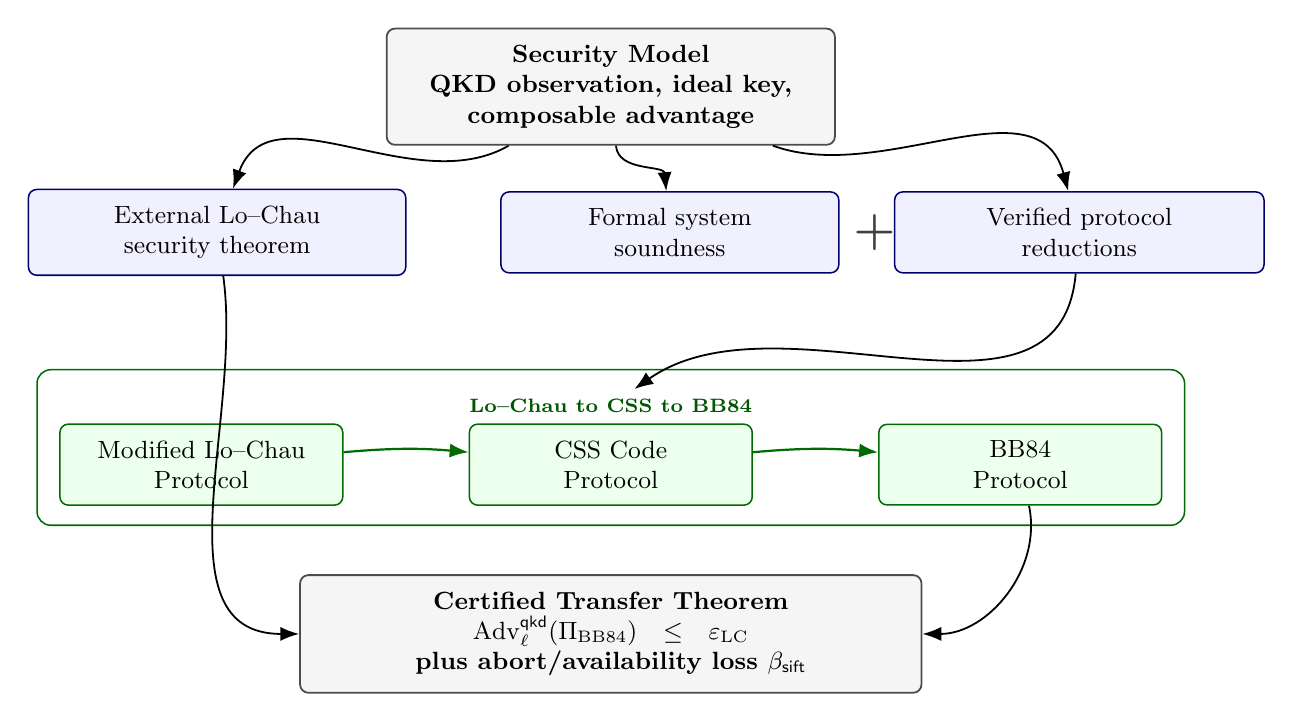
\begin{tikzpicture}[
      font=\small,
      box/.style={
        draw=black!58,
        rounded corners=3pt,
        align=center,
        inner xsep=7pt,
        inner ysep=6pt,
        minimum height=10mm
      },
      root/.style={
        box,
        fill=black!4,
        draw=black!70,
        line width=0.65pt,
        text width=52mm,
        font=\small\bfseries
      },
      proof/.style={
        box,
        fill=blue!6,
        draw=blue!42!black,
        line width=0.55pt,
        text width=43mm
      },
      game/.style={
        box,
        fill=green!7,
        draw=green!42!black,
        line width=0.55pt,
        text width=31mm
      },
      theorem/.style={
        box,
        fill=black!4,
        draw=black!70,
        line width=0.65pt,
        text width=74mm,
        font=\small\bfseries
      },
      group/.style={
        draw=green!42!black,
        rounded corners=5pt,
        inner xsep=8pt,
        inner ysep=7pt,
        line width=0.55pt
      },
      arr/.style={-{Latex[length=2.4mm]}, line width=0.65pt},
      chain/.style={-{Latex[length=2.4mm]}, line width=0.8pt, draw=green!42!black}
    ]
    \node[root] (model) at (4.6,0)
    {Security Model\\QKD observation, ideal key,\\composable advantage};
    
    \node[proof] (external) at (-0.4,-1.85)
    {External Lo--Chau\\security theorem};
    
    \node[proof, text width=38mm] (soundness) at (5.35,-1.85)
    {Formal system\\soundness};
    
    \node[font=\LARGE\bfseries, text=black!75] (plus) at (7.95,-1.85)
    {+};
    
    \node[proof, text width=42mm] (verified) at (10.55,-1.85)
    {Verified protocol\\reductions};
    
    \node[game] (lc) at (-0.6,-4.8)
    {Modified Lo--Chau\\Protocol};
    
    \node[game] (css) at (4.6,-4.8)
    {CSS Code\\Protocol};
    
    \node[game] (bb84) at (9.8,-4.8)
    {BB84\\Protocol};
    
    \node[font=\scriptsize\bfseries, text=green!34!black] (reductionTitle) at (4.6,-4.05)
    {Lo--Chau to CSS to BB84};
    \node[group, fit=(reductionTitle)(lc)(css)(bb84)] (reductionBox) {};
    
    \node[theorem] (transfer) at (4.6,-6.95)
    {Certified Transfer Theorem\\
    $\operatorname{Adv}^{\mathsf{qkd}}_{\ell}(\Pi_{\mathrm{BB84}})
    \leq \varepsilon_{\mathrm{LC}}$\\
    plus abort/availability loss $\beta_{\mathsf{sift}}$};
    
    \draw[arr] (model) to[out=210,in=70] (external);
    \draw[arr] (model) to[out=-85,in=95] (soundness);
    \draw[arr] (model) to[out=-20,in=105] (verified);
    \draw[arr] (verified) to[out=-95,in=35] (reductionTitle);
    \draw[chain] (lc) to[out=5,in=175] (css);
    \draw[chain] (css) to[out=5,in=175] (bb84);
    \draw[arr] (external) to[out=-82,in=180] (transfer);
    \draw[arr] (bb84) to[out=-78,in=0] (transfer);
    \end{tikzpicture}%
    }
    \caption{External Lo-Chau Protocol Security, Soundness of our Formal System, and Verified Protocol Reduction prove the Security of BB84 Protocol  automatically.}
    \Description{Document roadmap and certified protocol-reduction flow.}
    \label{fig:roadmap-certified-flow}
    \end{figure*}
    
\textcolor{red}{\textbf{We can use (Swap)+(Sift) to handle Check and Key bit choosing, but there are two choosing-----"Choosing Check\&Key and Choosing back after Channel" in Lo-Chau whlie only one choosing-----"Choosing after Channel" after BB84.}}

\clearpage

\section{Security Model and Main Statement}\label{security_theorem}
This section explains what the game-hopping proof proves and how it
implies QKD security.

The relational judgment
\[
\Xi
\vdash
P\sim_{\delta}P'
:
\Phi_{\mathcal V}
\Longrightarrow
\Psi_{\mathcal W}
\]
is a program-logic statement.  It is not, by itself, a QKD security
definition.  A game hop is interpreted as a
statement about the output of the two games.  Once the relational postcondition has been extracted as a statement about
terminal QKD observations, the trace-distance comparison transfers security
from the idealized protocol to the real protocol.

Throughout this section, \(\Delta_0\) ranges over well-typed initial classical-quantum states satisfying the initialization assumptions of the protocol, and
\[
U_{\textbf{channel}}
\]
ranges over  channel attacks.  A channel attack is a fixed joint unitary acting on the transmitted quantum systems in \textcolor{red}{the displayed bit order} together with the channel-side state and adversarial state. When two games are compared, the same \(\Delta_0\) and the same\(U_{\textbf{channel}}\) are used on both sides.

\begin{definition}[Terminal QKD Observation]

For a protocol program \(P\), the QKD observation we care about is the tuple
\[
\mathcal O_P
\stackrel{\triangle}{=}
(K_A^P,K_B^P,L^P,\mathsf E^P).
\]

Here \(K_A^P\) and \(K_B^P\) are Alice's and Bob's final key registers,
\(L^P\) is the authenticated public transcript retained in the terminal
observation, and \(\mathsf E^P\) is the final adversarial quantum system.
The system \(\mathsf E^P\) includes the adversary and all channel-side systems.

When the compared hop is the CSS phase-frame publication-elimination hop, the
transcript component retained in the QKD observation is the authenticated
transcript after removing the displayed \(z\)-publication cells, written
\(L^{P,\setminus z}\).  In that hop, the notation \(L^P\) in the terminal
observation means this retained transcript.  In all other hops,
\(L^{P,\setminus z}=L^P\).

When two games \(P\) and \(P'\) are compared, their terminal observations are
required to be output-compatible after this retained-transcript convention:
\[
K_A^P,K_B^P,L^P,\mathsf E^P
\]
and
\[
K_A^{P'},K_B^{P'},L^{P'},\mathsf E^{P'}
\]
are interpreted as the corresponding output registers
\[
K_A,K_B,L,\mathsf E .
\]
Thus the two terminal output states live on the same Hilbert space and their
trace distance is well defined.


For an initial state \(\Delta_0\) and a channel attack
\(U_{\textbf{channel}}\), define the real terminal output state of \(P\) by
\[
\mathsf{Real}_{P}^{U_{\textbf{channel}}}(\Delta_0)
\stackrel{\triangle}{=}
\tr_{\overline{\mathcal O_P}}
\left(
\sem{P[U_{\textbf{channel}}]}(\Delta_0)
\right).
\]

The notation \(P[U_{\textbf{channel}}]\) means that each displayed  \textcolor{red}{bit-order send syntax sugar} in \(P\) is interpreted using the fixed joint unitary \(U_{\textbf{channel}}\).  The trace \(\tr_{\overline{\mathcal O_P}}\) removes all registers not belonging to the QKD observation \(\mathcal O_P\).

Because
\[
\sem{\mathbf{abort}}(\Delta)=0,
\]
\(\mathsf{Real}_{P}^{U_{\textbf{channel}}}(\Delta_0)\) is generally a
subnormalized non-abort terminal output.  Branches that execute the core command
\(\mathbf{abort}\) contribute zero mass to this terminal observation.  Their
probability is recorded separately as an abort or availability loss.
\end{definition}

\begin{definition}[Ideal Key Replacement]
Let
\[
\tau^{=}_{K_AK_B}
\stackrel{\triangle}{=}
2^{-\ell}
\sum_{s\in\{0,1\}^{\ell}}
\ket{s,s}\bra{s,s}
\]
be the perfectly shared uniform \(\ell\)-bit key state.

For a terminal QKD state
\[
\rho_{K_AK_BL\mathsf E},
\]
define
\[
\mathsf{Ideal}_{\ell}(\rho)
\stackrel{\triangle}{=}
\tau^{=}_{K_AK_B}
\otimes
\tr_{K_AK_B}(\rho).
\]
Thus only the key registers \(K_A,K_B\) are replaced by an independent
perfectly shared uniform key.  The public transcript and adversarial system are
preserved.  If \(\rho\) is subnormalized, then
\(\mathsf{Ideal}_{\ell}(\rho)\) has the same trace as \(\rho\).
\end{definition}

\begin{definition}[Subnormalized Non-Abort QKD Secrecy Advantage]
For a protocol program \(P\), define its \(\ell\)-bit non-abort QKD secrecy
advantage by
\[
\operatorname{Adv}^{\mathsf{qkd}}_{\ell}(P)
\stackrel{\triangle}{=}
\sup_{\Delta_0,U_{\textbf{channel}}}
D\left(
\mathsf{Real}_{P}^{U_{\textbf{channel}}}(\Delta_0),
\mathsf{Ideal}_{\ell}
\left(
\mathsf{Real}_{P}^{U_{\textbf{channel}}}(\Delta_0)
\right)
\right),
\]
where
\[
D(\rho,\sigma)
\stackrel{\triangle}{=}
\frac12\|\rho-\sigma\|_1 .
\]
The supremum \(\sup_{\Delta_0,U_{\textbf{channel}}}\) is over the initial
states and channel attacks specified at the beginning of this section.

This is a subnormalized non-abort advantage. Branches that execute
\(\mathbf{abort}\) have already contributed zero mass to
\(\mathsf{Real}_{P}^{U_{\textbf{channel}}}(\Delta_0)\), and their probability
is reported separately.

Since the ideal key state \(\tau^{=}_{K_AK_B}\) has
\(K_A=K_B\), the same trace-distance term also charges non-abort
key-disagreement mass. Thus the advantage covers secrecy and agreement on the
non-abort terminal output.

A protocol is \(\varepsilon\)-secure in this sense when
\[
\operatorname{Adv}^{\mathsf{qkd}}_{\ell}(P)\leq\varepsilon .
\]
\end{definition}


\begin{definition}[Observational Hop]
Let \(P\) and \(P'\) be output-compatible protocol games.  We write
\[
\Xi
\vdash
P
\approx_{\eta}^{\mathsf{qkd}}
P'
\]
when the following data have been checked.

First, there is a resource-threaded relational derivation
\[
\Xi
\vdash
P\sim_{\delta}P'
:
\Phi_{\mathcal V}
\Longrightarrow
\Psi_{\mathcal W}.
\]
All rule-local side conditions used by the derivation are
semantically valid, and the left and right resource traces satisfy the
auxiliary live-view discipline.

Second, the terminal postcondition \(\Psi_{\mathcal W}\) is strong
enough to extract a trace-distance statement about the QKD observation:
\[
\sup_{\Delta_0,U_{\textbf{channel}}}
D\left(
\mathsf{Real}_{P}^{U_{\textbf{channel}}}(\Delta_0),
\mathsf{Real}_{P'}^{U_{\textbf{channel}}}(\Delta_0)
\right)
\leq
\eta .
\]

The number \(\delta\) is the internal loss parameter of the relational
judgment.  The number \(\eta\) is the external game-hop loss after the observation has been extracted.  They need not be identical:
if the extraction from \(\Psi_{\mathcal W}\) to trace distance changes
the bound, the final extracted bound is what is recorded as \(\eta\).

\end{definition}

\begin{lemma}[Observation Extraction]
Let \(P\) and \(P'\) be output-compatible games.  Suppose a valid
resource-threaded relational derivation for \(P\) and \(P'\) has a postcondition that identifies
\[
(K_A,K_B,L,\mathsf E)
\]
on the two sides up to extracted loss \(\eta\).  Then, for every
admissible \(\Delta_0\) and \(U_{\textbf{channel}}\),
\[
D\left(
\mathsf{Real}_{P}^{U_{\textbf{channel}}}(\Delta_0),
\mathsf{Real}_{P'}^{U_{\textbf{channel}}}(\Delta_0)
\right)
\leq
\eta .
\]
\end{lemma}

\begin{lemma}[Hop Composition]
If
\[
\Xi_i
\vdash
P_i
\approx_{\eta_i}^{\mathsf{qkd}}
P_{i+1}
\qquad
(0\leq i<N),
\]
then
\[
\sup_{\Delta_0,U_{\textbf{channel}}}
D\left(
\mathsf{Real}_{P_0}^{U_{\textbf{channel}}}(\Delta_0),
\mathsf{Real}_{P_N}^{U_{\textbf{channel}}}(\Delta_0)
\right)
\leq
\sum_{i=0}^{N-1}\eta_i .
\]
\end{lemma}

\begin{lemma}[Security Transfer with Separate Abort Loss]
Let \(P\) and \(P'\) be output-compatible games, and let \(F\) be a classical
event in \(P'\). Suppose
\[
\sup_{\Delta_0,U_{\textbf{channel}}}
\Pr_{P'}^{U_{\textbf{channel}}}[F]\leq \beta .
\]
Suppose every \(F\)-branch of \(P'\) executes the core command
\[
\mathbf{abort}.
\]
Suppose further that, on the compared terminal observation, the remaining
non-\(F\) restriction is represented by a classical trace-nonincreasing map
\(\mathcal R_{\neg F}\) that may restrict transcript, branch, and auxiliary
classical registers but does not modify the key values, and that for every
admissible \(\Delta_0\) and \(U_{\textbf{channel}}\),
\[
\mathsf{Real}_{P'}^{U_{\textbf{channel}}}(\Delta_0)
=
\mathcal R_{\neg F}
\left(
\mathsf{Real}_{P}^{U_{\textbf{channel}}}(\Delta_0)
\right)
\]
on the terminal QKD observation. Assume also that this restriction commutes
with ideal key replacement:
\[
\mathsf{Ideal}_{\ell}\circ \mathcal R_{\neg F}
=
\mathcal R_{\neg F}\circ \mathsf{Ideal}_{\ell}.
\]
Then
\[
\operatorname{Adv}^{\mathsf{qkd}}_{\ell}(P')
\leq
\operatorname{Adv}^{\mathsf{qkd}}_{\ell}(P).
\]

Indeed, for each admissible \(\Delta_0\) and \(U_{\textbf{channel}}\),
contractivity of trace distance gives
\[
D\left(
\mathcal R_{\neg F}(\rho),
\mathcal R_{\neg F}(\mathsf{Ideal}_{\ell}(\rho))
\right)
\leq
D\left(
\rho,
\mathsf{Ideal}_{\ell}(\rho)
\right),
\]
with
\(\rho=\mathsf{Real}_{P}^{U_{\textbf{channel}}}(\Delta_0)\).

The number \(\beta\) is reported separately as an abort or availability loss.
It is not added to the non-abort QKD secrecy advantage.

If an event is not implemented by the core abort command, then it is not an
availability-only event in this sense and must instead be accounted for as an
ordinary observational-hop loss.
\end{lemma}


\begin{theorem}[Certified Transfer of Lo--Chau Security to BB84]
Let
\[
P_0=\Pi_{\mathrm{LC}},
\qquad
P_N=\Pi_{\mathrm{BB84}} .
\]
Assume the certified game-hopping chain identifies the subnormalized terminal
QKD observations of \(P_0\) and \(P_N\) on the non-sifting-failure branch,
with \(L\) interpreted as the retained authenticated transcript.  In the CSS
\(z\)-publication elimination hop, this retained transcript is
\(L^{\setminus z}\).

Let
\[
Y
\stackrel{\triangle}{=}
\sum_{i=1}^{4n+\delta}
\mathbf 1[b[i]=b_2[i]]
\]
be the number of basis matches in the BB84 sifting step. Since Alice's and
Bob's basis strings are sampled independently of \(\Delta_0\) and
\(U_{\textbf{channel}}\),
\[
Y\sim \operatorname{Binomial}(4n+\delta,1/2).
\]
The sifting-failure event is
\[
\mathsf{sift\mbox{-}fail}
\equiv
(Y<2n).
\]
Hence
\[
\beta_{\mathsf{sift}}
\stackrel{\triangle}{=}
\sup_{\Delta_0,U_{\textbf{channel}}}
\Pr_{\Pi_{\mathrm{BB84}}}^{U_{\textbf{channel}}}
[\mathsf{sift\mbox{-}fail}]
=
2^{-(4n+\delta)}
\sum_{j=0}^{2n-1}
\binom{4n+\delta}{j}.
\]
By Hoeffding's inequality,
\[
\beta_{\mathsf{sift}}
\leq
\exp\left(
-\frac{\delta^2}{2(4n+\delta)}
\right).
\]

Assume that the \(\mathsf{sift\mbox{-}fail}\) branch executes the core command
\[
\mathbf{abort}.
\]
If
\[
\operatorname{Adv}^{\mathsf{qkd}}_{\ell}(\Pi_{\mathrm{LC}})
\leq
\varepsilon_{\mathrm{LC}},
\]
then
\[
\operatorname{Adv}^{\mathsf{qkd}}_{\ell}(\Pi_{\mathrm{BB84}})
\leq
\varepsilon_{\mathrm{LC}} .
\]
Moreover, the additional probability that BB84 aborts because too few sifted
positions are available is at most
\[
\beta_{\mathsf{sift}} .
\]
Thus, if one reports a combined security-plus-availability failure parameter,
it is bounded by
\[
\varepsilon_{\mathrm{LC}}+\beta_{\mathsf{sift}}.
\]
\end{theorem}

The generic observational-transfer bound and the sifting-failure bound
play different roles.  For a generic game-hop chain, if one only knows
\[
\sup_{\Delta_0,U_{\textbf{channel}}}
D\left(
\mathsf{Real}_{P_N}^{U_{\textbf{channel}}}(\Delta_0),
\mathsf{Real}_{P_0}^{U_{\textbf{channel}}}(\Delta_0)
\right)
\leq
\eta_{\mathsf{hop}},
\]
then the triangle inequality and contractivity of
\(\mathsf{Ideal}_{\ell}\) give the standard transfer estimate
\[
\operatorname{Adv}^{\mathsf{qkd}}_{\ell}(P_N)
\leq
\operatorname{Adv}^{\mathsf{qkd}}_{\ell}(P_0)
+
2\eta_{\mathsf{hop}} .
\]
One copy of \(\eta_{\mathsf{hop}}\) compares the real terminal states,
and the other copy compares their ideal key replacements.

The sifting-failure event in the theorem above is not used as such a generic
secrecy-loss term.  It is handled by the stronger semantic condition that the
\(\mathsf{sift\mbox{-}fail}\) branch executes the core command
\[
\mathbf{abort}.
\]
Since the primitive abort semantics contributes zero mass to the terminal QKD
observation, this event does not enter the subnormalized secrecy advantage.  It
contributes only to the probability that the BB84 execution aborts because too
few sifted positions are available.  Therefore
\(\beta_{\mathsf{sift}}\) is recorded separately as an availability or abort
loss, rather than being added to the composable QKD secrecy advantage.  If one
reports a single combined security-plus-availability parameter, the bound
becomes
\[
\varepsilon_{\mathrm{LC}}+\beta_{\mathsf{sift}}.
\]

% include Terminal QKD Observation, Ideal Key Replacement,
% Composable QKD security, Certified Observational Hop,
% three lemma, main theorem, and \beta_{\mathsf{sift}} explanation
\newpage
\section{Proof A: Formal System Soundness}

\subsection{Program Model}
\subsubsection{Syntax}

\begin{definition}[Variable Names to Address Indexes]
Before program execution, all physical locations are fixed. For each base
variable, its physical address list is fixed before execution:
\[
\overset{\textbf{Quantum variables}}{\overbrace{
\bar q \mapsto [1,\ldots,n_q]
}}
\qquad
\overset{\textbf{Probability distributions}}{\overbrace{
p \mapsto [1,\ldots,n_p]
}}
\qquad
\overset{\textbf{Classical variables}}{\overbrace{
x \mapsto [1,\ldots,n_x]
}} .
\]
The above intervals are physical addresses; they are fixed and are not
created, destroyed, or reordered during program execution.

A distinguished authenticated public transcript \(L\) is backed by a fixed
reserved block of classical physical addresses. We write
\[
\mathsf P_L\subseteq \mathsf P_C
\]
for this reserved block, where \(\mathsf P_L\) is the set of physical
addresses reserved for \(L\), and \(\mathsf P_C\) is the set of classical
physical addresses. Transcript addresses are ordinary classical physical
addresses, but they are reserved for value-copy publication and are disjoint
from all private classical and probability registers used by the protocol.


Addresses are defined as
\[
(\mathsf{Quantum}\quad \mathsf{Int})
\mid
(\mathsf{Probability}\quad \mathsf{Int})
\mid
(\mathsf{Classical}\quad \mathsf{Int}) .
\]
\end{definition}

\begin{definition}[Logical Lists, Length, and Descriptor Views]
An indexed object \(g\) is either a base indexed variable or a logical list
view built from existing indexed objects. Each indexed object has a descriptor
\[
\operatorname{desc}(g)=(\ell_g,\alpha_g),
\]
where \(\ell_g\in\mathbb N\) is the logical length of \(g\), and
\[
\alpha_g:\{1,\ldots,\ell_g\}\to \mathsf{addresses}
\]
maps logical positions to fixed physical addresses of the appropriate sort.

For a base indexed variable \(g\) with fixed physical address list
\([a_1,\ldots,a_N]\), we have
\[
\ell_g=N,\qquad \alpha_g(t)=a_t\quad(1\le t\le N).
\]

The primitive descriptor operation in the language is descriptor append.
It updates descriptors only. It does not create physical locations, does not
copy quantum states, and does not copy classical or probability values.

Protocol-level descriptor constructions such as fixed-size selection, \textcolor{red}{list formation by guarded append loops}, descriptor partitioning, and append loops are not primitive semantic constructs. When they are displayed in game hoppings, they are proof-oriented abbreviations to be expanded into

\[
\mathbf{shuffle},\quad
\mathbf{for}^{N},\quad
\mathbf{if},\quad
\mathbf{append},\quad
\mathbf{seq}
\]

before applying the denotational semantics.


For the auxiliary live-view discipline, these descriptor-construction
abbreviations may be checked either by their expansion or by the admissible
derived resource rules stated in \ref{resource_system}. These derived rules do not add
new program semantics. They only summarize the resource trace that would be
obtained by explicit proof-time splitting, singleton append, and dropping of
unused singleton roots.

Descriptor aliasing is allowed at the semantic level: two descriptor views may
denote overlapping physical addresses. The auxiliary live-view discipline in
\ref{resource_system} controls which descriptor views are live simultaneously.

The expression
\[
\mathbf{length}(g)
\]
denotes the current logical length \(\ell_g\). A reference \(g[i]\) is well
formed only when
\[
1\le i\le \ell_g,
\]
and is resolved to the fixed physical address
\[
\alpha_g(i).
\]
\end{definition}

\begin{definition}[Syntax]
Our programs are defined by the following syntax with quantum registers,
probability-distribution variables, typed indexed classical variables, and append:
\begin{align*}
    S ::=~&
    \textbf{skip}
    \mid \textbf{abort}
    \mid x[i] := E
    \mid p[i] :=_\$ \textbf{Coin-flip}_{\mu}
    \mid p :=_\$ \textbf{shuffle}(m)_{n}
    \mid~ \bar q[i] := \ket{0}
    \mid \bar q[i] \asteq U
    \\
    &\mid S_0;S_1
    \mid x[i] := \mathcal{M}[\bar q[j]]
    \mid
    \textbf{if } B \rightarrow S_0,\ \textbf{else}\rightarrow S_1
    \mid\mathbf{append}\ g'\ \mathbf{with}\ v .
\end{align*}
Here \(x[i]\) ranges over typed indexed classical locations, \(E\) ranges over
typed classical expressions, \(i,j,m,n\) range over expressions of type
\(\mathsf{Int}\), \(B\) ranges over classical predicates, \(g'\) ranges over
quantum, probability, or classical indexed objects, and \(v\) ranges over a
single compatible-sort variable.
The notation \(\bar q\) represents quantum variables
\(
\bar q[1],\ldots,\bar q[n],
\)
and \(p\) represents the probability-distribution variable
\(
(p[1],\ldots,p[n]).
\)

The assignment
\[
x[i]:=E
\]
is well formed only when \(x[i]\) and \(E\) have the same classical type. The
measurement assignment
\[
x[i]:=\mathcal M[\bar q[j]]
\]
is well formed only when \(x[i]\) has type \(\mathsf{Bit}\). All displayed multi-bit measurements, syndrome measurements, and basis-readout
blocks used in the protocol displays are syntax sugar for finite sequences of
bit-valued measurement assignments. No primitive multi-outcome measurement is
used by the displayed BB84 transfer proof.

For
\[
p:=_\$ \textbf{shuffle}(m)_{n},
\]
where \(0\le m\le n\), the probability-distribution variable \(p\) is
initialized uniformly over all bit strings of length \(n\) with exactly \(m\)
entries equal to \(1\):
\[
p:=_\$
\textbf{Uniform}
\left(
\left\{
s\in\{0,1\}^{n}
:
\sum_{r=1}^{n}s[r]=m
\right\}
\right).
\]

The command
\[
\mathbf{append}\ g'\ \mathbf{with}\ v
\]
is well formed only when \(g'\) and \(v\) have compatible sorts and the
corresponding resource judgment in \ref{resource_system} is derivable. It is descriptor
binding only. It does not copy, initialize, measure, or modify the underlying
value or quantum state.

The reserved transcript publication form
\[
L[\mathbf{next}] :=_{\mathsf{pub}} p[i]
\]
is not descriptor append and is not a linear aliasing primitive. It is the
reserved public-transcript value-copy command defined in
Definition~\ref{def:public-value-copy}. Displayed protocol programs may use it
only through authenticated-publication syntax sugar.

\textcolor{red}{The displayed bit-order send form is not a primitive command of the core syntax.  It is protocol-display syntax sugar for applying the fixed joint channel unitary \(U_{\textbf{channel}}\) to the displayed transmitted quantum registers in their displayed bit order, together with the channel-side and adversarial systems.  It introduces no new semantic construct and is expanded before the denotational semantics is applied.}
\end{definition}


\begin{definition}[Classical Expressions and Predicates]

Classical indexed variables are typed. We use
\[
\tau ::= \mathsf{Bit}\mid \mathsf{Int}
\]
for classical types, where
values of \(\mathsf{Bit}\) are inside \(
\mathbb B
\stackrel{\triangle}{=}
\{0,1\},\)
and values of \({\mathsf{Int}}\) are inside a finite, protocol-bounded set of integers. Each indexed classical variable \(x\) has a fixed entry type
\(\tau_x\), so every location \(x[i]\) has type \(\tau_x\). Probability-distribution variables are bit-valued indexed objects. Thus each
entry \(p[i]\) has type \(\mathsf{Bit}\).


Classical expressions are defined by
\[
E ::=
a
\mid x[i]
\mid \mathbf{length}(g)
\mid \mathbf{find~index}(X,E)
\mid E_1+E_2 .
\]
Here \(a\) ranges over integer constants and fixed protocol parameters;
\(x[i]\) ranges over typed indexed classical locations; \(g\) ranges over indexed objects for which a logical length is defined; and \(X\) ranges over
bit-valued indexed classical objects.

The type of a classical expression is determined as follows: \(\operatorname{type}(a)=\mathsf{Int}.\) \(\operatorname{type}(x[i])\) 
is the fixed type of the indexed classical location \(x[i]\). \(\operatorname{type}(\mathbf{length}(g))=\mathsf{Int}.\)
The expression \(\mathbf{find~index}(X,E)\)
is well formed only when \(X\) is bit-valued and
\(\operatorname{type}(E)=\mathsf{Int}\); in that case,
\(\operatorname{type}(\mathbf{find~index}(X,E))=\mathsf{Int}.\)
The expression \(E_1+E_2\) is well formed only when
\(\operatorname{type}(E_1)=\operatorname{type}(E_2)=\mathsf{Int};\)
in that case,
\(\operatorname{type}(E_1+E_2)=\mathsf{Int}.\)

The constants \(0\) and \(1\) may be used either as bit constants or as
integer constants; their intended type is determined by context.

Classical predicates are defined by
\[
B ::=
\top
\mid \bot
\mid E_1=E_2
\mid E_1<E_2
\mid E_1\leq E_2
\mid \neg B
\mid B_1\land B_2
\mid B_1\lor B_2 .
\]
The predicate \(E_1=E_2\) is well formed only when
\[
\operatorname{type}(E_1)=\operatorname{type}(E_2).
\]
The predicates \(E_1<E_2\) and \(E_1\leq E_2\) are well formed only when
\[
\operatorname{type}(E_1)=\operatorname{type}(E_2)=\mathsf{Int}.
\]
We use \(E_1\neq E_2,\quad
E_1>E_2,\quad
E_1\geq E_2\)
as standard abbreviations.
\end{definition}
% MOVE:  \section{Syntax and Rules}  \subsection{Syntax}

\subsubsection{Semantics}

\begin{definition}[Semantic Domains, Type Environment, and View Sorts]
Let
\[
\mathsf P
=
\mathsf P_Q
\;\cup\;
\mathsf P_P
\;\cup\;
\mathsf P_C
\]
be the fixed set of physical addresses, where
\[
\mathsf P_Q=\{(\mathsf{Quantum},t):1\le t\le n_q\},
\]
\[
\mathsf P_P=\{(\mathsf{Probability},t):1\le t\le n_p\},
\]
and
\[
\mathsf P_C=\{(\mathsf{Classical},t):1\le t\le n_x\}.
\]
As we said in syntax part, a fixed reserved transcript block
\[
\mathsf P_L\subseteq \mathsf P_C
\]
is used for public value-copy publication.

The quantum state space is fixed as
\[
\mathcal H_Q=\bigotimes_{\kappa\in\mathsf P_Q}\mathcal H_\kappa .
\]

A static type environment \(\Gamma_{\mathsf{ty}}\) is fixed before execution.
It assigns each classical physical address
\(\kappa\in \mathsf P_P\cup \mathsf P_C\)
a type in \(\{\mathsf{Bit},\mathsf{Int}\}\), where
\[
\mathsf{Val}_{\mathsf{Bit}}=\mathbb B=\{0,1\},
\]
and
\[
\mathsf{Val}_{\mathsf{Int}}
\]
is a finite protocol-bounded set of integers. Probability addresses are
bit-valued:
\[
\Gamma_{\mathsf{ty}}((\mathsf{Probability},t))=\mathsf{Bit}.
\]

A static view-sort environment is also \textbf{fixed} before execution. It assigns each
indexed object a sort:
\[
\operatorname{sort}(g)\in
\{
\mathsf{QReg},
\mathsf{PList},
\mathsf{CList}(\mathsf{Bit}),
\mathsf{CList}(\mathsf{Int})
\}.
\]
The expression \(\operatorname{sort}(g)\) is a fixed static function, not a
resource fact and not a runtime predicate.
\end{definition}


\begin{definition}[Stores, Logical Positions, and Physical Addresses]
A classical store \(\sigma\) assigns each classical physical address
\(\kappa\in\mathsf P_P\cup\mathsf P_C\) a value
\[
\sigma(\kappa)\in \mathsf{Val}_{\Gamma_{\mathsf{ty}}(\kappa)}.
\]
It also contains, for every indexed object \(g\), a descriptor
\[
\operatorname{desc}_{\sigma}(g)
=
(\ell_g^\sigma,\alpha_g^\sigma),
\qquad
\alpha_g^\sigma:\{1,\ldots,\ell_g^\sigma\}\to\mathsf P .
\]

The store \(\sigma\) is well typed under \(\Gamma_{\mathsf{ty}}\), written
\(\sigma\models\Gamma_{\mathsf{ty}}\), if every stored value has the type
prescribed by \(\Gamma_{\mathsf{ty}}\), and every descriptor respects the sort
of its indexed object:
\[
\operatorname{sort}(g)=\mathsf{QReg}
\Rightarrow
\alpha_g^\sigma(t)\in\mathsf P_Q,\quad
\operatorname{sort}(g)=\mathsf{PList}
\Rightarrow
\alpha_g^\sigma(t)\in\mathsf P_P,
\quad
\operatorname{sort}(g)=\mathsf{CList}(\tau)
\Rightarrow
\alpha_g^\sigma(t)\in\mathsf P_C
\text{ and }
\Gamma_{\mathsf{ty}}(\alpha_g^\sigma(t))=\tau .
\]

For a logical reference \(g[i]\), define its logical position by
\[
\operatorname{addr}_\sigma(g[i])
\stackrel{\triangle}{=}
\llbracket i\rrbracket_\sigma,
\]
and its resolved physical address by
\[
\mathsf{phys}_\sigma(g[i])
\stackrel{\triangle}{=}
\alpha_g^\sigma(\operatorname{addr}_\sigma(g[i]))
=
\alpha_g^\sigma(\llbracket i\rrbracket_\sigma).
\]
This is defined only when
\(1\le \llbracket i\rrbracket_\sigma\le \ell_g^\sigma\).
\end{definition}

\begin{definition}[Evaluation of Classical Expressions]
For a well-formed expression \(E\), its value in a well-typed store \(\sigma\)
is written \(\llbracket E\rrbracket_\sigma\). Integer constants and fixed
protocol parameters satisfy \(\llbracket a\rrbracket_\sigma=a\). For indexed
classical locations,
\[
\llbracket x[i]\rrbracket_\sigma
=
\sigma(\mathsf{phys}_\sigma(x[i])).
\]
For bit-valued indexed objects \(X\), \(\llbracket X[i]\rrbracket_\sigma\) is
defined in the same way.

Logical length is interpreted by
\[
\llbracket \mathbf{length}(g)\rrbracket_\sigma=\ell_g^\sigma.
\]
Index search is interpreted by
\[
\llbracket \mathbf{find~index}(X,E)\rrbracket_\sigma
=
\min\{t:t\ge \llbracket E\rrbracket_\sigma,\ 1\le t\le \ell_X^\sigma, X[t]=1\},
\]
whenever the set is nonempty. 

Integer addition is interpreted by
\[
\llbracket E_1+E_2\rrbracket_\sigma
=
\llbracket E_1\rrbracket_\sigma+
\llbracket E_2\rrbracket_\sigma,
\]
whenever the result lies in the finite protocol-bounded integer domain.
\end{definition}

\begin{definition}[Evaluation of Classical Predicates]
Satisfaction of a classical predicate \(B\) in a well-typed store \(\sigma\)
is written \(\sigma\models B\). It is defined by
\[
\sigma\models\top,\qquad \sigma\not\models\bot,
\quad
\sigma\models E_1=E_2
\Longleftrightarrow
\llbracket E_1\rrbracket_\sigma=\llbracket E_2\rrbracket_\sigma,
\quad
\sigma\models E_1<E_2
\Longleftrightarrow
\llbracket E_1\rrbracket_\sigma<\llbracket E_2\rrbracket_\sigma,
\]
and similarly for \(E_1\le E_2\). Boolean connectives are interpreted
classically:
\[
\sigma\models\neg B\Longleftrightarrow \sigma\not\models B,
\quad
\sigma\models B_1\land B_2
\Longleftrightarrow
\sigma\models B_1\text{ and }\sigma\models B_2,
\quad
\sigma\models B_1\lor B_2
\Longleftrightarrow
\sigma\models B_1\text{ or }\sigma\models B_2.
\]
\end{definition}

\begin{definition}[Classical-Quantum States]
A classical-quantum state is a sub-normalized mixed state of the form
\[
\Delta
=
\sum_{\sigma:\sigma\models\Gamma_{\mathsf{ty}}}
\mu(\sigma)\ket{\sigma}\bra{\sigma}\otimes\rho_\sigma,
\]
where \(\mu\) is a sub-distribution over well-typed stores,
\(\sum_{\sigma}\mu(\sigma)\le 1,\)
and, whenever \(\mu(\sigma)>0\),
\(\rho_\sigma\in D(\mathcal H_Q).\)
If \(\sum_\sigma\mu(\sigma)=1\), then \(\Delta\) is normalized.
\end{definition}

\begin{definition}[Program Semantics]
The denotational semantics of a program \(S\) is written
\(\llbracket S\rrbracket\). We write
\(\sigma[\kappa\mapsto v]\) for the store obtained from \(\sigma\) by
assigning value \(v\) to the physical classical address \(\kappa\), leaving all
other values and descriptors unchanged.

\[
\llbracket\mathbf{skip}\rrbracket(\Delta)=\Delta,
\qquad
\llbracket\mathbf{abort}\rrbracket(\Delta)=0.
\]

For classical assignment \(x[i]:=E\), let
\(\kappa_\sigma=\mathsf{phys}_\sigma(x[i]),
\quad
v_\sigma=\llbracket E\rrbracket_\sigma ,\)
then
\[
\llbracket x[i]:=E\rrbracket
\left(
\sum_\sigma\mu(\sigma)\ket{\sigma}\bra{\sigma}\otimes\rho_\sigma
\right)
=
\sum_\sigma
\mu(\sigma)
\ket{\sigma[\kappa_\sigma\mapsto v_\sigma]}
\bra{\sigma[\kappa_\sigma\mapsto v_\sigma]}
\otimes\rho_\sigma .
\]


For coin flip, let \(\kappa_\sigma=\mathsf{phys}_\sigma(p[i])\). Let
\(\mathsf{Coin}_{p[i]}^\sigma:\mathbb B\to[0,1]\) be the coin distribution
associated with \(p[i]\) in store \(\sigma\), satisfying
\(\sum_{b\in\mathbb B}\mathsf{Coin}_{p[i]}^\sigma(b)=1.\)
For each \(\omega\), define
\(\mu'(\omega)
=
\sum_{\substack{\sigma,\ b\in\mathbb B\\
\sigma[\kappa_\sigma\mapsto b]=\omega}}
\mu(\sigma)\mathsf{Coin}_{p[i]}^\sigma(b),\)
and, whenever \(\mu'(\omega)>0\),
\[
\rho'_\omega
=
\frac{1}{\mu'(\omega)}
\sum_{\substack{\sigma,\ b\in\mathbb B\\
\sigma[\kappa_\sigma\mapsto b]=\omega}}
\mu(\sigma)\mathsf{Coin}_{p[i]}^\sigma(b)\rho_\sigma .
\]
Then
\[
\llbracket p[i]:=_\$ \mathbf{Coin\mbox{-}flip}_{\mu}\rrbracket
\left(
\sum_\sigma\mu(\sigma)\ket{\sigma}\bra{\sigma}\otimes\rho_\sigma
\right)
=
\sum_{\omega:\mu'(\omega)>0}
\mu'(\omega)\ket{\omega}\bra{\omega}\otimes\rho'_\omega .
\]
For simplicity, we write $p[i]:=_{\$}\mu$ to express above single bit distribution assigning syntax.


For \(p:=_\$\mathbf{shuffle}(m)_n\), set
\(M_\sigma=\llbracket m\rrbracket_\sigma\) and
\(N_\sigma=\llbracket n\rrbracket_\sigma\), and define
\(\mathsf{Sh}_\sigma
=
\left\{
s\in\{0,1\}^{N_\sigma}:
\sum_{r=1}^{N_\sigma}s[r]=M_\sigma
\right\}.\)
For each output store \(\omega\), define
\(\mu'(\omega)
=
\sum_{\substack{\sigma,\ s\in\mathsf{Sh}_\sigma\\
\sigma[p\mapsto s]=\omega}}
\frac{\mu(\sigma)}{|\mathsf{Sh}_\sigma|},\)
and, whenever \(\mu'(\omega)>0\),
\[
\rho'_\omega
=
\frac{1}{\mu'(\omega)}
\sum_{\substack{\sigma,\ s\in\mathsf{Sh}_\sigma\\
\sigma[p\mapsto s]=\omega}}
\frac{\mu(\sigma)}{|\mathsf{Sh}_\sigma|}\rho_\sigma .
\]
Then
\[
\llbracket p:=_\$\mathbf{shuffle}(m)_n\rrbracket
\left(
\sum_\sigma\mu(\sigma)\ket{\sigma}\bra{\sigma}\otimes\rho_\sigma
\right)
=
\sum_{\omega:\mu'(\omega)>0}
\mu'(\omega)\ket{\omega}\bra{\omega}\otimes\rho'_\omega .
\]
Here \(\sigma[p\mapsto s]\) sets \(p[t]\) to \(s[t]\) for
\(1\le t\le N_\sigma\), updates \(\ell_p=N_\sigma\), and uses the fixed
physical probability addresses of \(p\).

For quantum initialization, let
\(\kappa_\sigma=\mathsf{phys}_\sigma(\bar q[i]).\)
Define
\[
\rho_\sigma^{0,\kappa_\sigma}
=
\ket 0_{\kappa_\sigma}\bra 0
\otimes
\operatorname{Tr}_{\kappa_\sigma}(\rho_\sigma),
\]
under the fixed tensor ordering of \(\mathcal H_Q\). Then
\[
\llbracket \bar q[i]:=\ket 0\rrbracket
\left(
\sum_\sigma\mu(\sigma)\ket{\sigma}\bra{\sigma}\otimes\rho_\sigma
\right)
=
\sum_\sigma
\mu(\sigma)\ket{\sigma}\bra{\sigma}
\otimes
\rho_\sigma^{0,\kappa_\sigma}.
\]

For unitary update, let \(\kappa_\sigma=\mathsf{phys}_\sigma(\bar q[i])\).
Then
\[
\llbracket \bar q[i]\asteq U\rrbracket
\left(
\sum_\sigma\mu(\sigma)\ket{\sigma}\bra{\sigma}\otimes\rho_\sigma
\right)
=
\sum_\sigma
\mu(\sigma)\ket{\sigma}\bra{\sigma}
\otimes
U_{\kappa_\sigma}\rho_\sigma U_{\kappa_\sigma}^{\dagger},
\]
where \(U_{\kappa_\sigma}\) acts on \(\kappa_\sigma\) and as identity elsewhere.

Sequential composition is interpreted by
\[
\llbracket S_0;S_1\rrbracket
=
\llbracket S_1\rrbracket\circ\llbracket S_0\rrbracket.
\]

For measurement assignment \(x[i]:=\mathcal M[\bar q[j]]\), assume
\(\mathcal M=\{M_0,M_1\}\). Let
\(\kappa_\sigma=\mathsf{phys}_\sigma(\bar q[j]),
\quad
c_\sigma=\mathsf{phys}_\sigma(x[i]).\)
For \(b\in\mathbb B\), define the unnormalized post-measurement state
\(\rho_{\sigma,b}
\stackrel{\triangle}{=}
M_{b,\kappa_\sigma}\rho_\sigma M_{b,\kappa_\sigma}^{\dagger}.\)
For each output store \(\omega\), define
\(\mu'(\omega)
=
\sum_{\substack{\sigma,\ b\in\mathbb B\\
\sigma[c_\sigma\mapsto b]=\omega}}
\mu(\sigma)\operatorname{Tr}(\rho_{\sigma,b}),\)
and, whenever \(\mu'(\omega)>0\),
\[
\rho'_\omega
=
\frac{1}{\mu'(\omega)}
\sum_{\substack{\sigma,\ b\in\mathbb B\\
\sigma[c_\sigma\mapsto b]=\omega}}
\mu(\sigma)\rho_{\sigma,b}.
\]
Then
\[
\llbracket x[i]:=\mathcal M[\bar q[j]]\rrbracket
\left(
\sum_\sigma\mu(\sigma)\ket{\sigma}\bra{\sigma}\otimes\rho_\sigma
\right)
=
\sum_{\omega:\mu'(\omega)>0}
\mu'(\omega)\ket{\omega}\bra{\omega}\otimes\rho'_\omega .
\]
For conditionals, define
\[
\Delta_B=
\sum_{\sigma:\sigma\models B}
\mu(\sigma)\ket{\sigma}\bra{\sigma}\otimes\rho_\sigma,
\qquad
\Delta_{\neg B}=
\sum_{\sigma:\sigma\not\models B}
\mu(\sigma)\ket{\sigma}\bra{\sigma}\otimes\rho_\sigma .
\]
Then
\[
\llbracket
\mathbf{if}\ B\rightarrow S_0,\ \mathbf{else}\rightarrow S_1
\rrbracket(\Delta)
=
\llbracket S_0\rrbracket(\Delta_B)
+
\llbracket S_1\rrbracket(\Delta_{\neg B}).
\]
The sum on the right-hand side is identified with its canonical
classical-quantum form by collecting equal output stores.


Logical-list operations update descriptors only.

For the primitive command
\[
\mathbf{append}\ g'\ \mathbf{with}\ v,
\]
where \(v\) is a single logical reference of compatible sort, let
\[
L=\ell_{g'}^\sigma,
\qquad
\kappa_\sigma=\mathsf{phys}_\sigma(v).
\]
The updated store \(\sigma'\) satisfies
\[
\ell_{g'}^{\sigma'}=L+1,
\qquad
\alpha_{g'}^{\sigma'}(t)=\alpha_{g'}^\sigma(t)\quad(1\le t\le L),
\qquad
\alpha_{g'}^{\sigma'}(L+1)=\kappa_\sigma.
\]
And it required that \(
\operatorname{sort}(g')=\operatorname{sort}(v)\). All ordinary classical values and all other descriptors are unchanged. This
operation aliases the resolved physical address. It does not copy the value or
state stored at that address.

Fixed-size selection, \textcolor{red}{list formation by guarded append loops}, descriptor partitioning, and append-loop syntax sugars are not primitive semantic clauses. In game displays they may be used as abbreviations, but before formal denotational interpretation they are expanded into shuffle, bounded for-loops, conditionals, sequential composition, and single append commands. 

\textcolor{red}{Likewise, the displayed bit-order send form has no separate semantic clause.  Before denotational interpretation, it is expanded to the ordinary multi-register unitary update that applies the fixed \(U_{\textbf{channel}}\) to the displayed transmitted registers in displayed bit order and to the channel-side and adversarial systems.}

\end{definition}

\begin{definition}[Public Value Copy]
\label{def:public-value-copy}
For public value-copy publication, let \(L\) be the transcript descriptor and
let
\[
\eta_L^\sigma
\]
be the next unused reserved transcript address in \(\mathsf P_L\). The reserved
command
\[
L[\mathbf{next}] :=_{\mathsf{pub}} p[i]
\]
is well formed only when \(p[i]\) is classical or probability-valued. It
produces a store \(\sigma'\) satisfying
\[
\sigma'(\eta_L^\sigma)
=
\sigma(\mathsf{phys}_\sigma(p[i])),
\]
extends the descriptor of \(L\) by the fresh transcript address
\[
\alpha_L^{\sigma'}(\ell_L^\sigma+1)=\eta_L^\sigma,
\]
and leaves the descriptor of \(p\) unchanged. Thus publication copies a value
into a fresh transcript cell and does not create descriptor aliasing with the
source location.
\end{definition}

\begin{definition}[Well-Formedness and Type Preservation]
The semantic function \(\llbracket S\rrbracket\) is defined only when
\(S\) is well formed with respect to the fixed type environment
\(\Gamma_{\mathsf{ty}}\), and only on stores \(\sigma\) satisfying
\(\sigma\models\Gamma_{\mathsf{ty}}\).

In particular,
\[
\operatorname{type}(x[i])=\operatorname{type}(E)
\quad\text{for }x[i]:=E,
\qquad
\operatorname{type}(x[i])=\mathsf{Bit}
\quad\text{for }x[i]:=\mathcal M[\bar q[j]],
\]
and every reference \(g[i]\) must satisfy
\[
1\le \llbracket i\rrbracket_\sigma\le \ell_g^\sigma.
\]
Moreover,
\[
0\le \llbracket m\rrbracket_\sigma\le \llbracket n\rrbracket_\sigma
\]
whenever \(\mathbf{shuffle}(m)_n\) is used.

For a bounded for-loop syntax sugar
\[
\mathbf{for}^{N}i=1\mathbf{~to~}E\quad S(i)\quad\mathbf{end},
\]
well-formedness is checked on its finite guarded expansion. The proof
obligations are
\[
\Xi\vDash 0\le E\le N
\]
and
\[
\forall\,1\le t\le N,\qquad
\operatorname{upd}(S(t))\cap\operatorname{acc}(E)=\emptyset.
\]
References inside \(S(t)\) are checked under the active guard \(t\le E\).

Displayed selection abbreviations in game hoppings are checked either after
expansion or by the admissible derived resource rules. Their size obligations
are ordinary assertion obligations; for example
\[
\Xi\vDash 0\le m\le E\le N
\]
for
\[
\mathbf{select}^{N}\ m\ \mathbf{from}\ E.
\]
The expression \(\mathbf{find~index}(X,E)\) is defined only when its search set
is nonempty.

For every multi-register quantum operation, the resolved quantum physical
addresses must be pairwise distinct and dimension-compatible.

The semantics preserves well-typed stores: if
\[
\Delta
=
\sum_{\sigma:\sigma\models\Gamma_{\mathsf{ty}}}
\mu(\sigma)\ket{\sigma}\bra{\sigma}\otimes\rho_\sigma
\quad\text{and}\quad
\llbracket S\rrbracket(\Delta)
=
\sum_{\omega}\mu'(\omega)\ket{\omega}\bra{\omega}\otimes\rho'_\omega,
\]
then
\[
\mu'(\omega)>0
\quad\Longrightarrow\quad
\omega\models\Gamma_{\mathsf{ty}}.
\]
\end{definition}
% MOVE:  \section{Syntax and Rules}  \subsection{Semantics}

\subsection{Resource and Relational Logic}

\subsubsection{\textbf{Auxiliary Live-View Discipline}}\label{resource_system}

The relational proof system never computes runtime descriptor maps or physical
addresses. Physical addresses appear only in the semantic soundness statement.
The auxiliary resource layer is therefore deliberately small: it tracks only
which linear logical root views are live at each program point.

The purpose of this layer is not to re-type the language and not to record
protocol facts such as filter weights, list lengths, or fixed-size sampling
properties. Static typing is fixed by \(\Gamma_{\mathsf{ty}}\) and by the
static view-sort environment
\[
\operatorname{sort}(g)\in
\{
\mathsf{QReg},
\mathsf{PList},
\mathsf{CList}(\mathsf{Bit}),
\mathsf{CList}(\mathsf{Int})
\}.
\]
The auxiliary layer enforces only the following invariant:
\[
\boxed{
\text{simultaneously live linear roots denote pairwise disjoint physical
addresses.}
}
\]

\begin{definition}[Linear Root Contexts]
A linear root context is a finite set
\[
\Omega=\{F_1,\ldots,F_k\}
\]
of live owned logical root views.

A root view \(F\) is an independently owned descriptor view. It may be
(i) a base indexed object,
(ii) a fresh empty logical list root,
(iii) a logical list root already populated by earlier descriptor appends, or
(iv) an owned subroot \(G|_I\) obtained by proof-time decomposition of an
owned root \(G\), where \(I\) is a finite set of logical positions of \(G\).

For an owned subroot \(G|_I\), let
\[
I=\{i_1<\cdots<i_s\}.
\]
Its descriptor is interpreted by
\[
\ell_{G|_I}^\sigma=s,
\qquad
\alpha_{G|_I}^\sigma(r)=\alpha_G^\sigma(i_r)
\quad(1\le r\le s).
\]
The sort of \(G|_I\) is inherited from \(G\). If \(I=\{i\}\), then
\(G|_{\{i\}}\) is an owned singleton root. It owns exactly the physical address
resolved by the original logical reference \(G[i]\).

The origin annotation of a subroot records where its addresses came from:
\[
\alpha_{G|_I}^\sigma(r)=\mathsf{phys}_\sigma(G[i_r]).
\]
This annotation is not ownership of the old root \(G\). If \(G\) is replaced by
its owned subroots in the resource context, then \(G\) itself is no longer live.

Thus, if \(g\in\Omega\), then \(g[i]\) is a live subview of \(g\), but it is
not an independently owned singleton root. Conversely, if \(g\) has been
decomposed and \(g|_{\{i\}}\in\Omega\), then the surface reference \(g[i]\)
may be used as a view owned by that singleton root. A context may not contain
both \(g\) and a nonempty owned subroot \(g|_I\), since that would violate
pairwise disjointness of distinct live roots.

Fresh empty logical list roots may be placed in \(\Omega\) before a descriptor
construction starts. Since their descriptors have length zero, they own no
physical addresses and are disjoint from all existing roots. This is a
well-formed context formation convention, not a program command and not a
resource rule.

We identify \(\operatorname{Own}(F)\) with membership \(F\in\Omega\). Thus the
notation \(\operatorname{Own}(F)\) is no longer a separate syntactic form.

Every root in \(\Omega\) has one of the linear sorts
\[
\mathsf{QReg},
\qquad
\mathsf{PList},
\qquad
\mathsf{CList}(\mathsf{Bit}),
\qquad
\mathsf{CList}(\mathsf{Int}).
\]
All three kinds of program data---quantum, probability, and classical indexed
data---are treated linearly by this auxiliary discipline.

The public transcript \(L\) is not a linear root in \(\Omega\); it is managed
by its fixed reserved transcript block and append-only publication discipline.
\end{definition}

\begin{definition}[Physical Interpretation of Root Contexts]
For an indexed object, logical list view, or owned subroot \(F\), define
\[
\mathsf{Phys}_{\sigma}(F)
=
\{\alpha_F^\sigma(t):1\le t\le \ell_F^\sigma\}.
\]
If \(F=G|_I\) and \(I=\{i_1<\cdots<i_s\}\), this means
\[
\mathsf{Phys}_{\sigma}(G|_I)
=
\{\alpha_G^\sigma(i_r):1\le r\le s\}.
\]
For a finite tuple of views, \(\mathsf{Phys}_{\sigma}\) is interpreted
componentwise and then unioned.

A store \(\sigma\) satisfies a root context \(\Omega\), written
\[
\sigma\models\Omega,
\]
iff every \(F\in\Omega\) is descriptor-well-formed and internally duplicate-free,
and any two distinct roots in \(\Omega\) are physically disjoint.

Descriptor-well-formedness means that every descriptor address respects the
static sort of its view. Internal duplicate-freeness means
\[
1\le r<s\le \ell_F^\sigma
\quad\Longrightarrow\quad
\alpha_F^\sigma(r)\ne\alpha_F^\sigma(s).
\]
This requirement applies uniformly to quantum, probability, and classical
linear views.

Pairwise disjointness of distinct roots means
\[
F,G\in\Omega,\quad F\ne G
\quad\Longrightarrow\quad
\mathsf{Phys}_{\sigma}(F)\cap\mathsf{Phys}_{\sigma}(G)=\emptyset.
\]
\end{definition}

\begin{definition}[Subview and Position-Disjointness]
The symbolic subview relation
\[
U\preceq F
\]
means that \(U\) is a valid logical subview of the currently owned root view
\(F\). It is generated by indexing, slicing, tuple projection, and by the
origin relation of owned subroots.

If \(F=G|_I\) with
\[
I=\{i_1<\cdots<i_s\},
\]
then the original surface reference \(G[i_r]\) is regarded as a subview of
\(F\):
\[
G[i_r]\preceq G|_I,
\qquad
\operatorname{pos}_{G|_I}(G[i_r])=\{r\}.
\]
Thus after decomposing \(G\), the old root \(G\) is not live, but its individual
surface references can still be used when they are owned by corresponding
live subroots.

If \(U\preceq F\), then \(\operatorname{pos}_F(U)\) denotes the set of logical
positions of \(F\) selected by \(U\). For example,
\[
\operatorname{pos}_g(g[i])=\{\llbracket i\rrbracket\},
\qquad
\operatorname{pos}_g(g[a{:}b])=\{a,\ldots,b\}.
\]
For an owned subroot \(g|_I\), positions are counted inside the subroot
descriptor, not inside the suspended source descriptor.

For symbolic expressions, a proof obligation such as
\[
\operatorname{pos}_F(U)\cap\operatorname{pos}_F(V)=\emptyset
\]
is derived from the current resource context and ordinary symbolic arithmetic
facts. Distinct live roots are disjoint. Subviews of the same live root are
disjoint only when their selected positions are disjoint, as known at that
program point.

We write
\[
\Omega\vdash_{\mathsf{res}} U\# V
\]
when \(U\) and \(V\) are provably physically disjoint under \(\Omega\). This
judgment is generated by two cases.

First, disjoint live roots are disjoint:
\[
\frac{
U\preceq F
\qquad
V\preceq G
\qquad
F,G\in\Omega
\qquad
F\ne G
}{
\Omega\vdash_{\mathsf{res}} U\# V
}.
\]

Second, position-disjoint subviews of the same internally duplicate-free root
are disjoint:
\[
\frac{
U\preceq F
\qquad
V\preceq F
\qquad
F\in\Omega
\qquad
\operatorname{pos}_F(U)\cap\operatorname{pos}_F(V)=\emptyset
}{
\Omega\vdash_{\mathsf{res}} U\# V
}.
\]

For finite view sets \(\mathcal U,\mathcal V\), the judgment
\[
\Omega\vdash_{\mathsf{res}}\mathcal U\#\mathcal V
\]
means pairwise disjointness of every component of \(\mathcal U\) from every
component of \(\mathcal V\).
\end{definition}


\begin{definition}[Liveness]
A logical view \(U\) is live under \(\Omega\), written
\[
\Omega\vdash_{\mathsf{res}}\operatorname{Live}(U),
\]
iff it is a subview of some currently owned root:
\[
\exists F\in\Omega.\ U\preceq F.
\]
For a finite view set \(\mathcal U\),
\[
\Omega\vdash_{\mathsf{res}}\operatorname{Live}(\mathcal U)
\]
means that every component of \(\mathcal U\) is live.

A suspended descriptor may still exist in the semantic store, but it is not
live. It may not be used as a program reference, assertion index, frame view,
or rule-local side-condition view.
\end{definition}

\begin{definition}[Access and Update Views]
For a program fragment \(S\), the proof-time view set
\[
\operatorname{acc}(S)
\]
collects the logical views that \(S\) reads, writes, measures, initializes,
applies unitary operations to, or uses to resolve descriptor addresses.

The proof-time view set
\[
\operatorname{upd}(S)
\]
collects the logical views whose stored values or quantum states are modified
by \(S\). Descriptor-update targets are included as update views for descriptor
operations.

These are not program constructs and not functions available in the programming
language. They are meta-level summaries used only to state liveness and
disjointness obligations. They refine the phrase ``\(S\) is disjoint from a
frame'' into either access-disjointness or update-disjointness.

For the primitive commands,
\[
\operatorname{acc}(x[i]:=E)=\{x[i]\}\cup\operatorname{acc}(E),
\qquad
\operatorname{upd}(x[i]:=E)=\{x[i]\},
\]
\[
\operatorname{acc}(p[i]:=_\$\mathbf{Coin\mbox{-}flip})=\{p[i]\},
\qquad
\operatorname{upd}(p[i]:=_\$\mathbf{Coin\mbox{-}flip})=\{p[i]\},
\]
\[
\operatorname{acc}(p:=_\$\mathbf{shuffle}(m)_n)=
\{p\}\cup\operatorname{acc}(m)\cup\operatorname{acc}(n),
\qquad
\operatorname{upd}(p:=_\$\mathbf{shuffle}(m)_n)=\{p\},
\]
\[
\operatorname{acc}(\bar q[\mathbf i]\asteq U)=\{\bar q[\mathbf i]\},
\qquad
\operatorname{upd}(\bar q[\mathbf i]\asteq U)=\{\bar q[\mathbf i]\},
\]
\[
\operatorname{acc}(x[i]:=\mathcal M[\bar q[j]])
=
\{x[i],\bar q[j]\},
\qquad
\operatorname{upd}(x[i]:=\mathcal M[\bar q[j]])
=
\{x[i],\bar q[j]\}.
\]

\textcolor{red}{For a displayed bit-order send syntax sugar}
\[\textcolor{red}{\mathbf{send}_{\mathsf{bit}}(\vec u)}\]\textcolor{red}{where \(\vec u=(u_1,\ldots,u_M)\) is the displayed tuple of transmitted quantum views, its proof-time access and update summaries are}\[\textcolor{red}{\operatorname{acc}\left(\mathbf{send}_{\mathsf{bit}}(\vec u)\right)=\{u_1,\ldots,u_M\},\qquad\operatorname{upd}\left(\mathbf{send}_{\mathsf{bit}}(\vec u)\right)=\{u_1,\ldots,u_M\}.}
\]
\textcolor{red}{The displayed tuple order is the bit order used in the expansion to the fixed \(U_{\textbf{channel}}\).}

For the primitive descriptor append command,
\[
\operatorname{acc}(\mathbf{append}\ g'\ \mathbf{with}\ v)=\{g',v\},
\qquad
\operatorname{upd}(\mathbf{append}\ g'\ \mathbf{with}\ v)=\{g'\}.
\]

For sequencing and conditionals, both summaries are defined by union over the
subprograms, with the conditional guard included in \(\operatorname{acc}\).
For bounded for-loop syntax sugars and all other syntax sugar,
\(\operatorname{acc}\) and \(\operatorname{upd}\) are computed from the finite
expanded program.

\textcolor{red}{Selection, partition, append-loop syntax sugars, bit-order send syntax sugar, and syndrome-measurement syntax sugars are not primitive access/update forms. For frame and swap reasoning, their access/update summaries are those of their finite expansions, except that the displayed bit-order send form may use the explicit tuple summary above. For resource-threading, descriptor-construction syntax sugars may instead be discharged by the admissible derived resource rules below, the bit-order send form may be discharged by \({\rm Res\mbox{-}BitSend}\), and syndrome-measurement syntax sugars may be discharged by the admissible syndrome resource rule below.}


For convenience, if \(h\in\{0,1\}^{N}\), write
\[
\bar r|_h
\stackrel{\triangle}{=}
\{\bar r[t]:h_t=1\}.
\]
Then the access/update summaries of the displayed check measurements are
\[
\operatorname{acc}
\left(
s:=\mathsf{MeasZCheck}_{h}(\bar r;a)
\right)
=
\bar r|_h\cup\{a,s\},
\qquad
\operatorname{upd}
\left(
s:=\mathsf{MeasZCheck}_{h}(\bar r;a)
\right)
=
\bar r|_h\cup\{a,s\},
\]
and
\[
\operatorname{acc}
\left(
s:=\mathsf{MeasXCheck}_{h}(\bar r;a)
\right)
=
\bar r|_h\cup\{a,s\},
\qquad
\operatorname{upd}
\left(
s:=\mathsf{MeasXCheck}_{h}(\bar r;a)
\right)
=
\bar r|_h\cup\{a,s\}.
\]

For a displayed CSS syndrome measurement,
\[
(s_Z,s_X):=
\mathsf{CSSSyn}_{H_Z,H_X}(\bar r;a_Z,a_X),
\]
we use
\[
\operatorname{acc}
=
\{\bar r,a_Z,a_X,s_Z,s_X\},
\qquad
\operatorname{upd}
=
\{\bar r,a_Z,a_X,s_Z,s_X\},
\]
understood as abbreviations for the corresponding finite expansion into
initialization, Hadamard gates, CNOT gates, sequencing, and binary
single-qubit measurements.

For a classical expression or predicate \(R\),
\(\operatorname{acc}(R)\) is the set of indexed views read by \(R\), and
\(\operatorname{upd}(R)=\emptyset\).
For paired fragments, we write
\[
\operatorname{acc}(P,P')=(\operatorname{acc}(P),\operatorname{acc}(P')),
\qquad
\operatorname{upd}(P,P')=(\operatorname{upd}(P),\operatorname{upd}(P')).
\]
\end{definition}


\begin{definition}[Auxiliary Resource Judgment]
The auxiliary statement judgment is
\[
\vdash_{\mathsf{res}}S: \Omega\rightarrow\Omega'.
\]
It is used only after the ordinary static syntax, type, and bounded-expansion
checks for \(S\) have been discharged. The judgment itself records only live
root ownership, liveness of accessed views, and the ownership transfer caused
by descriptor-aliasing commands.

The judgment does not re-type the language, does not store list lengths, filter
weights, construction facts, or protocol arithmetic, and does not record
well-formedness facts in \(\Omega\). Those facts belong to the static program
model, assertion entailments, or syntax-sugar admissibility checks.

It only means that \(S\) is statically well formed, all its program references are
live when used, and execution transforms the live root context \(\Omega\) into
\(\Omega'\).

\end{definition}


\paragraph{Alias-neutral primitive commands.}

Let \(\mathsf{AliasPrim}\) be the set of commands that may update values,
quantum states, or descriptor lengths, but do not create descriptor aliases and
do not transfer ownership:
\[
x[i]:=E,\qquad
p[i]:=_\$ \mathbf{Coin\mbox{-}flip},\qquad
p:=_\$\mathbf{shuffle}(m)_n,
\qquad
\bar q[i]:=\ket0,
\qquad
\bar q[\mathbf i]\asteq U,
\qquad
x[i]:=\mathcal M[\bar q[j]].
\]

\textcolor{red}{The displayed bit-order send form is not a primitive member of \(\mathsf{AliasPrim}\).  It is a syntax sugar checked either by expanding it to the ordinary multi-register unitary update using \(U_{\textbf{channel}}\), or by the admissible derived rule \({\rm Res\mbox{-}BitSend}\) below.}

\[
\text{\rm (Res-Prim)}
\quad
\frac{
S\in\mathsf{AliasPrim}
\qquad
\Omega\vdash_{\mathsf{res}}\operatorname{Live}(\operatorname{acc}(S))
\qquad
\operatorname{QDistinct}_{\Omega}(S)
}{
\vdash_{\mathsf{res}}S:\Omega\rightarrow\Omega
}.
\]


Here \(\operatorname{QDistinct}_{\Omega}(S)\) is \(\top\) unless \(S\)
applies one quantum operation to an ordered tuple
\((u_1,\ldots,u_k)\) of quantum views with \(k\ge 2\). In that case,
\(\operatorname{QDistinct}_{\Omega}(S)
\quad\text{means}\quad
\Omega\vdash_{\mathsf{res}} u_r\#u_s
\quad(1\le r<s\le k).\)
Thus the same physical quantum system cannot be used twice as
arguments of one multi-register quantum operation.

\[
\text{\rm (Res-Skip)}
\quad
\vdash_{\mathsf{res}}\mathbf{skip}:\Omega\rightarrow\Omega .
\]

\[
\text{\rm (Res-Abort)}
\quad
\vdash_{\mathsf{res}}\mathbf{abort}: \Omega\rightarrow\Omega'
\]
for any \(\Omega'\). This is sound because \(\mathbf{abort}\) produces no
nonzero output store.

\[
\text{\rm (Res-Seq)}
\quad
\frac{
\vdash_{\mathsf{res}}S_0: \Omega\rightarrow\Omega_1
\qquad
\vdash_{\mathsf{res}}S_1: \Omega_1\rightarrow\Omega_2
}{
\vdash_{\mathsf{res}}S_0;S_1: \Omega\rightarrow\Omega_2
}.
\]

\[
\text{\rm ({Res-If})}
\quad
\frac{
\Omega\vdash_{\mathsf{res}}\operatorname{Live}(\operatorname{acc}(B))
\qquad
\vdash_{\mathsf{res}}S_0:\Omega\rightarrow\Omega'
\qquad
\vdash_{\mathsf{res}}S_1:\Omega\rightarrow\Omega'
}{
\vdash_{\mathsf{res}}
\mathbf{if}\ B\rightarrow S_0,\ \mathbf{else}\rightarrow S_1
:\Omega\rightarrow\Omega'
}.
\]

\paragraph{Resource decomposition and suspension.}

A proof-time split refinement
\[
\Omega\rightsquigarrow_{\mathsf{split}}\Omega^\sharp
\]
means that \(\Omega^\sharp\) is obtained from \(\Omega\) by replacing one or
more live roots \(G\) by owned subroots
\[
G|_{I_1},\ldots,G|_{I_s},
\]
where
\[
I_1\cup\cdots\cup I_s=\{1,\ldots,\ell_G\},
\qquad
I_a\cap I_b=\emptyset\quad(a\ne b).
\]
The sets \(I_1,\ldots,I_s\) are symbolic position sets and must form a
partition of the source root positions. This partition condition is a
side condition of the split refinement, not a fact stored in
\(\Omega\). Once the refinement is applied, the resulting subroots are
the live owned roots in \(\Omega^\sharp\); their physical disjointness
follows from the partition condition and the well-formedness of the
source root \(G\).

This split is not a program command. It does not update descriptors, values,
or quantum states. It only refines live ownership.

\[
\text{\rm (Res-Split)}
\quad
\frac{
\Omega\rightsquigarrow_{\mathsf{split}}\Omega^\sharp
\qquad
\vdash_{\mathsf{res}}S:\Omega^\sharp\rightarrow\Omega'
}{
\vdash_{\mathsf{res}}S:\Omega\rightarrow\Omega'
}.
\]

The rule is sound because every store satisfying \(\Omega\) also satisfies
\(\Omega^\sharp\): owned subroots are position-disjoint subviews of an
internally duplicate-free live root.

The proof may also suspend live roots that are no longer needed.

\[
\text{\rm (Res-Drop)}
\quad
\frac{
\vdash_{\mathsf{res}}S:\Omega\rightarrow\Omega_1
\qquad
\Omega'\subseteq\Omega_1
}{
\vdash_{\mathsf{res}}S:\Omega\rightarrow\Omega'
}.
\]

Dropping a root does not delete a descriptor from the semantic store. It only
removes the root from the live ownership context. Suspended descriptors may
still exist semantically, but they cannot be used as live program references,
assertion views, frame views, or disjointness witnesses.

\paragraph{Single append.}

\[
\text{\rm (Res-Append)}
\quad
\frac{
g'\in\Omega
\qquad
u\in\Omega
\qquad
u\text{ is an owned singleton root}
\qquad
v\preceq u
\qquad
g'\ne u
}{
\vdash_{\mathsf{res}}
\mathbf{append}\ g'\ \mathbf{with}\ v
:\Omega\rightarrow
\Omega-\{u\}
}.
\]

The source \(v\) must be backed by an independent live singleton root \(u\).
It is not enough that \(v\) is merely a subview of a larger live root. Thus,
from \(g\in\Omega\), one cannot derive
\[
\vdash_{\mathsf{res}}
\mathbf{append}\ g'\ \mathbf{with}\ g[i]
:\Omega\rightarrow
\Omega'
\]
while \(g\) remains live. If a proof needs to append the element denoted by
\(g[i]\), the resource context must first be refined so that the corresponding
physical address is owned by a singleton root, and then that singleton root is
consumed by \({\rm Res\mbox{-}Append}\).

Since \(g'\) and \(u\) are distinct live roots, they are disjoint before the
append. Since \(u\) is consumed by the rule, extending \(g'\)'s descriptor
preserves internal duplicate-freeness and does not introduce a second live
owner for the appended address.

This rule is a linear ownership transfer for descriptor aliasing. It does not
create a physical location, copy a value, copy a quantum state, or measure any
quantum system.

\paragraph{Derived descriptor-construction resource rules.}

The following rules are admissible derived rules of the auxiliary resource
system. They are not primitive semantic rules. Each rule abbreviates a finite
resource derivation obtained by proof-time splitting of source roots into owned
singleton roots, 
\textcolor{red}{applying \({\rm Res\mbox{-}Append}\) on the guarded branches that keep the current source position, and applying \({\rm Res\mbox{-}Drop}\) on branches that do not keep it.}

The auxiliary resource layer does not inspect stored filter values and does not
record branch sizes. It only records that each source position is visited at
most once, and that every visited source singleton is either transferred to an
output descriptor root or dropped.

For readability, write
\[
\mathsf{App}_{\vec h}(\vec v)
\stackrel{\triangle}{=}
\mathbf{append}\ h_1\ \mathbf{with}\ v_1;\
\cdots;\
\mathbf{append}\ h_r\ \mathbf{with}\ v_r .
\]

Let \(J\subseteq\{0,1\}\) be a nonempty set of kept branches. For each
\(d\in J\), let
\[
\vec h_d=(h_{d,1},\ldots,h_{d,r})
\]
be fresh empty roots. Define the branch body
\[
T_d(i)
\stackrel{\triangle}{=}
\begin{cases}
\mathsf{App}_{\vec h_d}(g_1[i],\ldots,g_r[i]),
& d\in J,\\
\mathbf{skip},
& d\notin J.
\end{cases}
\]
Thus branch \(1\) is the branch where the displayed guard holds, and branch
\(0\) is the else branch.

\[
\text{\rm (Res-SelectLoop)}
\quad
\frac{
\begin{array}{c}
g_1,\ldots,g_r\in \Omega\\
J\subseteq\{0,1\},\quad J\ne\emptyset\\
h_{d,1},\ldots,h_{d,r}\text{ are fresh empty roots}
\quad(d\in J,\ 1\le k\le r)
\end{array}
}{
\begin{array}{c}
\vdash_{\mathsf{res}}
\mathbf{for}^{N}i=1\mathbf{~to~}E
\quad
\mathbf{if}\ B(i)\rightarrow T_1(i),
\ \mathbf{else}\rightarrow T_0(i)
\quad
\mathbf{end}
:\\
\Omega\rightarrow\Omega+
\{h_{d,k}:d\in J,\ 1\le k\le r\}
-\{g_1,\ldots,g_r\}
\end{array}
}
\]
\[
\Xi\vDash \mathsf{Fit}_N(E;g_1,\ldots,g_r).
\]

The case \(J=\{1\}\) keeps only the true branch and drops the false branch.
The case \(J=\{0\}\) is symmetric. The case \(J=\{0,1\}\) keeps both branches.

The displayed guard \(B(i)\) is required to be a well-formed
classical predicate whose accessed views are live at the loop point.
This is the ordinary \({\rm Res\mbox{-}If}\) obligation.

Displayed fixed-size selection is an admissible abbreviation for shuffle
followed by the one-branch instance of \({\rm Res\mbox{-}SelectLoop}\). If the
displayed selection samples its filter into the live filter root \(a\), then

\[
\text{\rm (Res-Select)}
\quad
\frac{
\begin{array}{c}
a,g_1,\ldots,g_r\in \Omega\\
g'_1,\ldots,g'_r\text{ are fresh empty roots}\\
\end{array}
}{
\vdash_{\mathsf{res}}
g'_1,\ldots,g'_r
:=
\mathbf{select}^{N}\ m\ \mathbf{from}\ E\ \mathbf{for}\ g_1,\ldots,g_r
:\Omega\rightarrow
\Omega+\{g'_1,\ldots,g'_r\}-\{g_1,\ldots,g_r\}
}
\]
\[
\Xi\vDash
\mathsf{SelFit}_N(m,E;g_1,\ldots,g_r).
\]

Here \(a\) remains live. The source roots \(g_1,\ldots,g_r\) are suspended, and
the selected roots \(g'_1,\ldots,g'_r\) become live.

Soundness follows by expanding the displayed construction into primitive
commands. The expansion splits each source root into owned singletons, evaluates
the displayed branch condition, transfers the current singleton to the
corresponding kept output roots when the branch is kept, and drops it otherwise.
Thus no physical address has two distinct live owners.

\paragraph{\textcolor{red}{Derived resource rule for bit-order send syntax sugar.}}

\textcolor{red}{Let}
\[\textcolor{red}{\vec u=(u_1,\ldots,u_M)}\]
\textcolor{red}{be the displayed bit-ordered tuple of transmitted quantum views.  The following rule is admissible because the bit-order send form expands to the ordinary multi-register unitary update applying the fixed \(U_{\textbf{channel}}\) to the displayed transmitted tuple in displayed bit order.}

\[\textcolor{red}{\text{\rm (Res-BitSend)}\quad\frac{\Omega\vdash_{\mathsf{res}}\operatorname{Live}(\vec u)\qquad\Omega\vdash_{\mathsf{res}}u_r\#u_s\quad(1\le r<s\le M)}{\vdash_{\mathsf{res}}\mathbf{send}_{\mathsf{bit}}(\vec u):\Omega\rightarrow\Omega}.}\]

\textcolor{red}{This rule creates no descriptor alias and transfers no ownership.  It does not inspect a filter, and does not implement selection by channel reordering.  Selection, if present, must already have been represented by ordinary descriptor construction before the displayed tuple is sent.}


\paragraph{Publication.}

\[
\text{\rm (Res-Publish)}
\quad
\frac{
\Omega\vdash_{\mathsf{res}}\operatorname{Live}(p[i])
}{
\vdash_{\mathsf{res}}
L[\mathbf{next}] :=_{\mathsf{pub}} p[i]
:\Omega\rightarrow
\Omega
}.
\]


The transcript \(L\) is not a linear root in \(\Omega\). Publication
copies the current value of \(p[i]\) into the next unused reserved
transcript address. It does not append the physical address of \(p[i]\), does
not create descriptor aliasing, and does not consume the source view.

\paragraph{Fixed CSS classical input and syntax sugar.}

The CSS matrices, decoder tables, encoding conventions, and classical
post-processing maps used by the protocol are fixed external classical input.
They are not program variables, are not sampled by the language, and are not
inspected by the auxiliary resource system.

The names
\[
\mathbf{Encode},
\qquad
\mathbf{Decode},
\qquad
\mathbf{Encode}_{x,z},
\qquad
QEC,
\qquad
\mathsf{qecAlice},
\qquad
\mathsf{qecBob},
\qquad
D_X,
\qquad
D_Z
\]
are not primitive commands.

The unitary abbreviations
\[
\mathbf{Encode},
\qquad
\mathbf{Decode},
\qquad
\mathbf{Encode}_{x,z}
\]
are fixed classically indexed unitary syntax sugar. They are interpreted by the
ordinary unitary-update semantics and the classically indexed unitary syntax
sugar from Appendix~\ref{app:syntax-sugar}.

The classical maps
\[
\mathsf{qecAlice},
\qquad
\mathsf{qecBob},
\qquad
D_X,
\qquad
D_Z
\]
are fixed finite classical-map syntax sugar. They expand into bounded finite
case analysis and constant assignments. Their algebraic correctness is not a
resource fact; it is part of the fixed CSS error-correction assumptions in
Appendix~\ref{app:css-correction}.

The syndrome abbreviations
\[
\mathsf{MeasZCheck}_{h},
\qquad
\mathsf{MeasXCheck}_{h},
\qquad
\mathsf{CSSSyn}_{H_Z,H_X}
\]
are syntax sugar expanded into initialization, Hadamard gates, CNOT gates,
sequencing, and bit-valued single-qubit measurement.

The correction abbreviation
\[
\bar u := QEC(\bar r)
\]
is the CSS-QEC syntax sugar defined in
Definition~\ref{def:css-qec-sugar}. Its expansion uses only CSS syndrome
measurement syntax sugar, fixed finite classical-map syntax sugar, classically
indexed Pauli updates, and fixed CSS decoding.

Thus none of these names adds a primitive semantic construct.

\paragraph{Derived resource rule for CSS syndrome syntax sugar.}

For a quantum data block \(\bar r\), ancilla blocks \(a_Z,a_X\), and
bit-valued classical syndrome registers \(s_Z,s_X\), write
\[
\operatorname{AncFresh}_{\Omega}(\bar r;a_Z,a_X)
\]
to mean that all entries of \(a_Z\) and \(a_X\) are live quantum views,
pairwise disjoint, and disjoint from every quantum view in \(\bar r\). This is
a resource-side freshness condition only; it does not create any physical
qubit.

The following rule is admissible because the CSS syndrome abbreviation expands
into a finite sequence of \({\rm Res\mbox{-}Prim}\),
\({\rm Res\mbox{-}Seq}\), and bounded-loop resource derivations.

\[
\text{\rm (Res-CSSSyn)}
\quad
\frac{
\Omega\vdash_{\mathsf{res}}
\operatorname{Live}(\bar r,a_Z,a_X,s_Z,s_X)
\qquad
\operatorname{AncFresh}_{\Omega}(\bar r;a_Z,a_X)
}{
\vdash_{\mathsf{res}}
(s_Z,s_X):=
\mathsf{CSSSyn}_{H_Z,H_X}(\bar r;a_Z,a_X)
:
\Omega\rightarrow\Omega
}.
\]

This rule introduces no descriptor alias. The data block \(\bar r\) may be
updated because syndrome measurement is a projective measurement on \(\bar r\).
The ancillas are initialized and measured, and the classical syndrome registers
are assigned bit values.

\paragraph{Resource check for CSS-QEC syntax sugar.}

The abbreviation
\[
\bar u := QEC(\bar r)
\]
is resource-checked by expanding Definition~\ref{def:css-qec-sugar}. The
resulting resource trace uses only \({\rm Res\mbox{-}Prim}\),
\({\rm Res\mbox{-}Seq}\), \({\rm Res\mbox{-}If}\),
\({\rm Res\mbox{-}CSSSyn}\), and the finite case expansions for fixed unitary
families and fixed classical maps.

No descriptor alias is created by the correction steps. Any output view
\(\bar u\) used by the abbreviation is either a live decoded subview of the
corrected block or a fixed fresh output block specified by the CSS correction
convention and related to the corrected block by fixed unitary wiring.

\subsubsection{\textbf{Relational Judgment System}}
\begin{definition}[Symbolic Proof Context]
The symbolic proof context \(\Xi\) contains persistent non-resource
facts used in assertion entailments and protocol-specific lemmas,
such as protocol-parameter facts, arithmetic facts, name assumptions, and the
external CSS-code correctness assumptions stated in
Appendix~\ref{app:css-correction}.

Live-root ownership, liveness, disjointness, and resource state are
tracked separately by \(\Omega\). They are not assumptions in
\(\Xi\). A relational derivation is admissible only when it is
resource-threaded by suitable left and right \(\Omega\)-traces.

Thus resource judgments have the form
\[
\vdash_{\mathsf{res}}S:\Omega\rightarrow\Omega',
\]
while assertion entailments have the form
\[
\Xi\vDash \Phi\Longrightarrow\Psi.
\]
\end{definition}

\begin{definition}[Paired Logical Views]
A paired logical view is a finite list
\[
\mathcal V=
[(u_1,u'_1),\ldots,(u_m,u'_m)],
\]
where \(u_i\) is a logical reference or logical list view in the left program,
and \(u'_i\) is the corresponding logical reference or logical list view in
the right program.

Given stores \(\sigma,\sigma'\), resolution is componentwise:
\[
\mathsf{phys}_{\sigma,\sigma'}(u,u')
=
\left(
\mathsf{phys}_{\sigma}(u),
\mathsf{phys}_{\sigma'}(u')
\right).
\]
For list views, this is interpreted pointwise.

A paired view is well formed at a relational proof point when the left
components are live and well formed in the current left resource context, the
right components are live and well formed in the current right resource
context, and the paired components have matching lengths and compatible sorts.

No disjointness is required between a left physical address and a right physical
address: the two sides live in different store copies and different Hilbert
spaces. Disjointness obligations are checked componentwise within each side.
\end{definition}



\begin{definition}[View-Indexed Assertions]
An assertion \(A_{\mathcal V}\) is a projective predicate indexed by a paired
logical view \(\mathcal V\). For stores \(\sigma,\sigma'\), its branchwise
interpretation is
\(\llbracket A_{\mathcal V}\rrbracket_{\sigma,\sigma'}
\stackrel{\triangle}{=}
A_{\mathsf{phys}_{\sigma,\sigma'}(\mathcal V)}.\)
The corresponding projector on c-q states is the block-diagonal operator
\[
\llbracket A_{\mathcal V}\rrbracket
\stackrel{\triangle}{=}
\sum_{\sigma,\sigma'}
\ket{\sigma,\sigma'}\bra{\sigma,\sigma'}
\otimes
\llbracket A_{\mathcal V}\rrbracket_{\sigma,\sigma'}.
\]
Here
\(\ket{\sigma,\sigma'}=\ket{\sigma}\otimes\ket{\sigma'}\), and
\(A_{\mathsf{phys}_{\sigma,\sigma'}(\mathcal V)}\) is extended by identity
on all unmentioned quantum systems.

For projective assertions \(\Phi,\Psi\), define
\[
\Phi\land\Psi
\stackrel{\triangle}{=}
\operatorname{proj}
\left(
\operatorname{Im}(\Phi)\cap\operatorname{Im}(\Psi)
\right),
\qquad
\Phi\lor\Psi
\stackrel{\triangle}{=}
\operatorname{proj}
\left(
\operatorname{Im}(\Phi)+\operatorname{Im}(\Psi)
\right),
\qquad
\neg\Phi\stackrel{\triangle}{=}I-\Phi.
\]
If \(\Phi\Psi=0\), then
\[
\Phi\lor\Psi=\Phi+\Psi.
\]

The basic equality assertion on a paired logical view is written
\[
\equiv_{\mathcal V}.
\]
For a pair of classical logical references \(z,z'\) of the same finite value
domain \(D\), define
\[
\equiv^{D}_{(z,z')}
\stackrel{\triangle}{=}
\sum_{\substack{\sigma,\sigma'\\
\sigma(\mathsf{phys}_{\sigma}(z))
=
\sigma'(\mathsf{phys}_{\sigma'}(z'))\in D}}
\ket{\sigma,\sigma'}\bra{\sigma,\sigma'}
\otimes I_Q .
\]
When \(D\) is clear from the type of \(z,z'\), we write
\(\equiv_{(z,z')}\)
instead of \(\equiv^{D}_{(z,z')}\).

For probability-distribution entries \(p[i],p'[j]\), the assertion
\[
\equiv_{(p[i],p'[j])}
\]
means lockstep equality of the sampled branch value:
\(\qquad\sigma(\mathsf{phys}_{\sigma}(p[i]))
=
\sigma'(\mathsf{phys}_{\sigma'}(p'[j])).\)
For a distribution \(\mu\), we can define
\(\qquad\equiv^{\mu}_{(p[i],p'[j])}
\stackrel{\triangle}{=}
\equiv^{\operatorname{supp}(\mu)}_{(p[i],p'[j])}.\)

For a pair of quantum logical references \(\bar q[i],\bar q'[j]\),
\[
\equiv_{(\bar q[i],\bar q'[j])}
\]
denotes symmetric quantum equality on the resolved physical quantum systems.
That is, it is interpreted by the symmetric-space projector
\[
=_{\mathrm{sym}}
=
\frac{1}{2}(I\otimes I+\mathsf{SWAP})
\]
on the two resolved Hilbert spaces, extended by identity on all unmentioned
systems.

For list views, equality is defined pointwise:
\[
\equiv_{(g[1,\ldots,n],g'[1,\ldots,n])}
\stackrel{\triangle}{=}
\bigwedge_{t=1}^{n}
\equiv_{(g[t],g'[t])}.
\]

When the view is clear from context, we write simply \(\equiv\).
\end{definition}


\begin{definition}[Separable States]
We write
\[
\operatorname{Sep}D(\mathcal H_1:\mathcal H_2)
\]
for the set of separable density operators on
\(\mathcal H_1\otimes\mathcal H_2\), i.e.,
\[
\operatorname{Sep}D(\mathcal H_1:\mathcal H_2)
\stackrel{\triangle}{=}
\left\{
\rho\in D(\mathcal H_1\otimes\mathcal H_2)
:
\rho=\sum_{\ell}\lambda_{\ell}\sigma_{\ell}\otimes\tau_{\ell}
\right\},
\]
where
\[
\lambda_{\ell}\geq 0,\qquad
\sum_{\ell}\lambda_{\ell}=1,\qquad
\sigma_{\ell}\in D(\mathcal H_1),\qquad
\tau_{\ell}\in D(\mathcal H_2).
\]
We also use the sub-normalized separable cone
\(\operatorname{Sep}D_{\leq}(\mathcal H_1:\mathcal H_2)\)
defined by
\[
\operatorname{Sep}D_{\leq}(\mathcal H_1:\mathcal H_2)
\stackrel{\triangle}{=}
\left\{
\rho\in D_{\leq}(\mathcal H_1\otimes\mathcal H_2)
:
\rho=\sum_{\ell}\lambda_{\ell}\sigma_{\ell}\otimes\tau_{\ell}
\right\},
\]
where
\[
\lambda_{\ell}\geq 0,\qquad
\sum_{\ell}\lambda_{\ell}\leq 1,\qquad
\sigma_{\ell}\in D(\mathcal H_1),\qquad
\tau_{\ell}\in D(\mathcal H_2).
\]
\end{definition}


\begin{definition}[Rule-Local Side Conditions]
Side conditions are not threaded as a global context. They are semantic
premises of the particular rule that uses them. For example
\[
\mathcal M_1\approx \mathcal M_2,
\qquad
\operatorname{Sep}(\mathcal U:\mathcal F).
\]


For a measurement condition
\(\mathcal M_1\approx \mathcal M_2\), where
\(\qquad\mathcal M_1=\{M_{1,b}\}_{b\in\mathbb B},
\qquad
\mathcal M_2=\{M_{2,b}\}_{b\in\mathbb B},\) the two measurements induce the same outcome distribution on the
left and right input classical-quantum states \(\Delta_L,~\Delta_R\). We have the witness between them as \(\pi\), write
\[
\Delta_L\stackrel{\triangle}{=}\operatorname{Tr}_R(\pi),
\qquad
\Delta_R\stackrel{\triangle}{=}\operatorname{Tr}_L(\pi),
\]
this means
\[
\operatorname{Tr}
\left(
M_{1,b}\Delta_L M_{1,b}^{\dagger}
\right)
=
\operatorname{Tr}
\left(
M_{2,b}\Delta_R M_{2,b}^{\dagger}
\right)
\qquad
(b\in\mathbb B).
\]

A separability side condition
\[
\operatorname{Sep}(\mathcal U:\mathcal F)
\]
is well formed only when \(\mathcal U\) and \(\mathcal F\) are disjoint
quantum logical views. In each classical store-pair branch of witness \(\pi\), the corresponding
quantum state is separable between the resolved systems of
\(\mathcal U\) and \(\mathcal F\).
\end{definition}


\begin{definition}[Approximate Classical-Quantum Lifting]
Let
\[
\Delta
=
\sum_{\sigma}
\mu_1(\sigma)\ket{\sigma}\bra{\sigma}\otimes\rho_\sigma,
\qquad
\Delta'
=
\sum_{\omega}
\mu_2(\omega)\ket{\omega}\bra{\omega}\otimes\rho'_\omega
\]
be two c-q states. For a view-indexed projector \(A_{\mathcal V}\), we write
\[
\Delta\ A_{\mathcal V}^{\delta}\ \Delta'
\]
if there exists a witness
\[
\pi
=
\sum_{\sigma,\omega}
\nu(\sigma,\omega)
\ket{\sigma}\bra{\sigma}
\otimes
\ket{\omega}\bra{\omega}
\otimes
\rho_{\sigma,\omega},
\]
where
\(\rho_{\sigma,\omega}\in
D(\mathcal H_L\otimes\mathcal H_R),\)
such that
\[
\operatorname{Tr}_R(\pi)=\Delta,
\qquad
\operatorname{Tr}_L(\pi)=\Delta',
\]
and
\[
\operatorname{Tr}
\left(
\llbracket A_{\mathcal V}\rrbracket\pi
\right)
\ge
\operatorname{Tr}(\pi)-\delta.
\]
Here \(\operatorname{Tr}_L\) and \(\operatorname{Tr}_R\) trace out the whole left
or right side, including both the classical store register and the quantum
Hilbert space. When \(\delta=0\), we write
\[
\Delta\ A_{\mathcal V}\ \Delta'.
\]
\end{definition}

\begin{definition}[Classical-Quantum Relational Judgment]
A relational judgment has the form
\[
\Xi
\vdash
P\sim_{\delta}P'
:
\Phi_{\mathcal V}
\Longrightarrow
\Psi_{\mathcal W}.
\]



It is valid iff for every pair of well-typed c-q states
\(\Delta,\Delta'\), whenever there exists a witness \(\pi\) for the exact
lifting
\[
\Delta\ \Phi_{\mathcal V}\ \Delta'
\]
such that
\[
\operatorname{Tr}_R(\pi)=\Delta,
\qquad
\operatorname{Tr}_L(\pi)=\Delta',
\qquad
\operatorname{supp}_{\mathsf{cl}}(\pi)\models\Xi\quad\text{means satisfying all classical facts in} \quad\Xi,
\]
and
\[
\operatorname{Tr}
\left(
\llbracket \Phi_{\mathcal V}\rrbracket\pi
\right)
=
\operatorname{Tr}(\pi),
\]
then
\[
\llbracket P\rrbracket(\Delta)
\ \Psi_{\mathcal W}^{\delta}\
\llbracket P'\rrbracket(\Delta')
\]
holds.

The parameter \(\delta\in\mathbb R_{\ge 0}\) bounds the probability mass
violating the postcondition. When \(\delta=0\), we write
\[
\Xi
\vdash
P\sim P'
:
\Phi_{\mathcal V}
\Longrightarrow
\Psi_{\mathcal W}.
\]
\end{definition}


\begin{definition}[Assertion Entailment]
We write
\[
\Xi
\vDash
\Phi_{\mathcal V}
\Longrightarrow
\Psi_{\mathcal W}
\]
if for every witness \(\pi\) satisfying
\({\operatorname{supp}_{\mathsf{cl}}(\pi)\models\Xi},\)
we have
\[
\operatorname{Tr}
\left(
\llbracket\Phi_{\mathcal V}\rrbracket\pi
\right)
=
\operatorname{Tr}(\pi)
\quad\Longrightarrow\quad
\operatorname{Tr}
\left(
\llbracket\Psi_{\mathcal W}\rrbracket\pi
\right)
=
\operatorname{Tr}(\pi).
\]
Equivalently, for projective predicates this is branchwise image inclusion
under the symbolic assumptions in \(\Xi\).
\end{definition}

\begin{definition}[Resource-Threaded Relational Derivation]
Displayed relational rules suppress the auxiliary resource contexts. A
relational derivation is resource-threaded if there exist left and right
resource traces assigning a current live-root context to every program point in
the derivation.

For every program fragment \(S\) appearing on the left side of a rule, there
must be contexts \(\Omega_L,\Omega'_L\) such that
\[
\vdash_{\mathsf{res}}S:\Omega_L\rightarrow\Omega'_L.
\]
For every program fragment \(S'\) appearing on the right side, there must be
contexts \(\Omega_R,\Omega'_R\) such that
\[
\vdash_{\mathsf{res}}S':\Omega_R\rightarrow\Omega'_R.
\]

Every relational assertion rule and every rule-local side condition used at a
program point is interpreted with respect to the current left and right
resource contexts. All logical views mentioned by that rule or side condition
must be live at the corresponding program point. Every displayed disjointness
side condition is interpreted using the current resource context. Thus
\[
\Xi\vdash \mathcal U\#\mathcal V
\]
in a displayed relational rule means that, at the relevant proof point,
\[
\Omega_L\vdash_{\mathsf{res}}\mathcal U_L\#\mathcal V_L
\quad\text{and}\quad
\Omega_R\vdash_{\mathsf{res}}\mathcal U_R\#\mathcal V_R
\]
for the left and right components that occur.

The displayed relational rules do not inspect descriptor maps or physical
addresses. Their liveness and symbolic disjointness obligations are discharged
by the current \(\Omega\)-contexts.

\textcolor{red}{Descriptor append is a primitive program fragment. Displayed descriptor constructions such as fixed-size selection, dynamic-bounded selection, partition-style append loops, and guarded append loops are not primitive semantic constructs. A resource-threaded derivation may either expand them explicitly into shuffle, bounded for-loops, conditionals, sequential composition, and singleton append commands, or discharge them using the admissible derived resource rules \({\rm Res\mbox{-}Select}\) and \({\rm Res\mbox{-}SelectLoop}\).}

\textcolor{red}{The displayed bit-order send form is likewise not a primitive semantic construct. It may either be expanded to the ordinary multi-register unitary update using the fixed \(U_{\textbf{channel}}\) on the displayed transmitted tuple in displayed bit order, or be resource-checked using \({\rm Res\mbox{-}BitSend}\).}

\end{definition}



\textbf{Structural proof rules for QKD:}

\[
\text{\rm (Conseq)}
\quad
\frac{
\Xi
\vDash
\Phi'_{\mathcal V'}
\Longrightarrow
\Phi_{\mathcal V}
\qquad
\Xi
\vDash
\Psi_{\mathcal W}
\Longrightarrow
\Psi'_{\mathcal W'}
\qquad
\delta\leq\delta'
\qquad
\Xi
\vdash
P\sim_{\delta}P':
\Phi_{\mathcal V}
\Longrightarrow
\Psi_{\mathcal W}
}{
\Xi
\vdash
P\sim_{\delta'}P':
\Phi'_{\mathcal V'}
\Longrightarrow
\Psi'_{\mathcal W'}
}.
\]

\[
\text{\rm (Weaken-\(\Xi\))}
\quad
\frac{
\Xi
\vdash
P\sim_{\delta}P':
\Phi\Longrightarrow\Psi
\qquad
\Xi'\vDash\Xi
}{
\Xi'
\vdash
P\sim_{\delta}P':
\Phi\Longrightarrow\Psi
}.
\]

\[
\text{\rm (Seq)}
\quad
\frac{
\Xi
\vdash
P_0\sim_{\delta}P_1:
\Phi\Longrightarrow\Theta
\qquad
\Xi
\vdash
P'_0\sim_{\delta'}P'_1:
\Theta\Longrightarrow\Psi
}{
\Xi
\vdash
P_0;P'_0
\sim_{\delta+\delta'}
P_1;P'_1
:
\Phi\Longrightarrow\Psi
}.
\]

\[
\text{\rm (Skip)}
\quad
\Xi
\vdash
\mathbf{skip}\sim\mathbf{skip}:
\Phi\Longrightarrow\Phi .
\]

\[
\text{\rm (Abort)}
\quad
\Xi
\vdash
\mathbf{abort}\sim\mathbf{abort}:
\Phi\Longrightarrow\Psi .
\]

\[
\text{\rm (Ident)}
\quad
{
\Xi
\vdash
P\sim P:
\equiv_{\operatorname{acc} (P)}
\Longrightarrow
\equiv_{\operatorname{upd} (P)}
}.
\]

\[
\text{\rm (Comp)}
\quad
\frac{
\Xi
\vdash
P\sim_{\delta_1}P':
\equiv_{\mathcal V}
\Longrightarrow
\equiv_{\mathcal V}
\qquad
\Xi
\vdash
P'\sim_{\delta_2}P'':
\equiv_{\mathcal V}
\Longrightarrow
\equiv_{\mathcal V}
}{
\Xi
\vdash
P\sim_{\delta_1+\delta_2}P'':
\equiv_{\mathcal V}
\Longrightarrow
\equiv_{\mathcal V}
}.
\]


A frame assertion \(C_{\mathcal U}\) is a view-indexed projective assertion
indexed by the logical view \(\mathcal U\). 

\[
\text{\rm (Classical-Frame)}
\quad
\frac{
\Xi
\vdash
P\sim_{\delta}P':
\Phi\Longrightarrow\Psi
\qquad
C_{\mathcal U}\text{ is a classical frame assertion}
\qquad
\Xi\vdash
\mathcal U
\#
\operatorname{upd}(P,P')
}{
\Xi
\vdash
P\sim_{\delta}P':
\Phi\land C_{\mathcal U}
\Longrightarrow
\Psi\land C_{\mathcal U}
}.
\]

\[
\text{\rm (Quantum-Frame)}
\quad
\frac{\begin{array}{c}
\Xi
\vdash
P\sim_{\delta}P':
\Phi\Longrightarrow\Psi
\qquad\\
C_{\mathcal U}\text{ is a quantum frame assertion}
\qquad\\
\Xi\vdash
\mathcal U\#\operatorname{acc}(P,P')
\qquad
\Xi\vDash
\operatorname{Sep}(\mathcal U:\mathcal F)
\end{array}}{
\Xi
\vdash
P\sim_{\delta}P':
\Phi\land C_{\mathcal U}
\Longrightarrow
\Psi\land C_{\mathcal U}
}.
\]


where \(\mathcal F\) denotes the quantum logical views occurring in
\(\operatorname{acc}(P,P')\).

\[
\text{\rm (Swap)}
\quad
\frac{
\Xi\vdash
\operatorname{acc}(P_0)\#
\operatorname{acc}(P_1)
}{
\Xi
\vdash
P_0;P_1
\sim
P_1;P_0
:
\equiv_{\mathcal V}
\Longrightarrow
\equiv_{\mathcal V}
}.
\]



\textbf{Construct-Specific rules for QKD proof:}

For a classical logical reference \(z\) and a value \(a\), we write
\(\ket a_z\bra a\)
for the diagonal projector onto the store branches where \(z\) has value \(a\).
For paired classical logical references \(z,z'\), we write
\(\ket a_z\bra a\otimes\ket b_{z'}\bra b\)
for the corresponding projector on paired store branches.

For a positive operator \(T\), \(\operatorname{proj}(T)\) denotes the
orthogonal projector onto \(\operatorname{supp}(T)\). We use
\(\operatorname{Tr}_{z}(A)\) and \(\operatorname{Tr}_{z,z'}(A)\) for the
partial trace over the indicated logical views.

\[
\text{\rm (Assign-Const)}
\quad
\Xi
\vdash
x[i]:=a_1
\sim
x'[j]:=a_2
:
\Phi
\Longrightarrow
\ket{a_1}_{x[i]}\bra{a_1}
\land
\ket{a_2}_{x'[j]}\bra{a_2}
\land
\operatorname{proj}
\left(
\operatorname{Tr}_{x[i],x'[j]}(\Phi)
\right).
\]

\[
\text{\rm (Assign-Const-L)}
\quad
\Xi
\vdash
x[i]:=a
\sim
\mathbf{skip}
:
\Phi
\Longrightarrow
\ket a_{x[i]}\bra a
\land
\operatorname{proj}
\left(
\operatorname{Tr}_{x[i]}(\Phi)
\right).
\]

\[
\text{\rm (Init-Quantum)}
\quad
\Xi
\vdash
\bar q[i]:=\ket 0
\sim
\bar q'[j]:=\ket 0
:
\Phi
\Longrightarrow
\ket 0_{\bar q[i]}\bra 0
\land
\ket 0_{\bar q'[j]}\bra 0
\land
\operatorname{proj}
\left(
\operatorname{Tr}_{\bar q[i],\bar q'[j]}(\Phi)
\right).
\]

\[
\text{\rm (Init-Quantum-L)}
\quad
\Xi
\vdash
\bar q[i]:=\ket 0
\sim
\mathbf{skip}
:
\Phi
\Longrightarrow
\ket 0_{\bar q[i]}\bra 0
\land
\operatorname{proj}
\left(
\operatorname{Tr}_{\bar q[i]}(\Phi)
\right).
\]



For a distribution \(\mu\) over a finite set \(D\), and for a classical
logical reference \(z\), define
\[
\Pi_z^\mu
\stackrel{\triangle}{=}
\sum_{a\in\operatorname{supp}(\mu)}
\ket a_z\bra a .
\]
For paired classical logical references \(z,z'\), define
\[
\equiv^\mu_{(z,z')}
\stackrel{\triangle}{=}
\sum_{a\in\operatorname{supp}(\mu)}
\ket a_z\bra a
\otimes
\ket a_{z'}\bra a .
\]

\[
\text{\rm (Coin)}
\quad
\Xi
\vdash
p[i]:=_{\$}\mathbf{Coin\mbox{-}flip}_{\mu}
\sim
p'[j]:=_{\$}\mathbf{Coin\mbox{-}flip}_{\mu}
:
\Phi
\Longrightarrow
\equiv^{\mu}_{(p[i],p'[j])}
\land
\operatorname{proj}
\left(
\operatorname{Tr}_{p[i],p'[j]}(\Phi)
\right).
\]

\[
\text{\rm (Coin-L)}
\quad
\Xi
\vdash
p[i]:=_{\$}\mathbf{Coin\mbox{-}flip}_{\mu}
\sim
\mathbf{skip}
:
\Phi
\Longrightarrow
\Pi^\mu_{p[i]}
\land
\operatorname{proj}
\left(
\operatorname{Tr}_{p[i]}(\Phi)
\right).
\]

\[
\text{\rm (Shuffle)}
\quad
\frac{
\Xi
\vDash
\Phi\Longrightarrow m=m'\land n=n'
}{
\Xi
\vdash
p:=_{\$}\mathbf{shuffle}(m)_n
\sim
p':=_{\$}\mathbf{shuffle}(m')_{n'}
:
\Phi
\Longrightarrow
\equiv_{(p[1,\ldots,n],p'[1,\ldots,n'])}
\land
\operatorname{proj}
\left(
\operatorname{Tr}_{p[1,\ldots,n],p'[1,\ldots,n']}(\Phi)
\right)
}.
\]

For a distribution \(\mu\), define list equality with support restriction by
\[
\equiv^{\mu}_{(p[1,\ldots,N],p'[1,\ldots,N])}
\stackrel{\triangle}{=}
\bigwedge_{t=1}^{N}
\equiv^{\mu}_{(p[t],p'[t])}.
\]

\[
\text{\rm (IID)}
\quad
\frac{
\Xi\vDash\Phi\Longrightarrow  N=N'
}{
\Xi
\vdash
p:=_{\$}\mathbf{iid}_{\mu}(N,f)
\sim
p':=_{\$}\mathbf{iid}_{\mu}(N',f')
:
\Phi
\Longrightarrow
\equiv^{\mu}_{(p[1,\ldots,N],p'[1,\ldots,N'])}
\land
\operatorname{proj}
\left(
\operatorname{Tr}_{p[1,\ldots,N],p'[1,\ldots,N']}(\Phi)
\right)
}.
\]

The same rule may also be used for a finite sequence of iid samplers whose
common scheduling filter is sampled on one side before the sequence and on the
other side after the sequence:
\[
\text{\rm (IID)}
\quad
\frac{
\begin{array}{c}
\Xi\vDash\Phi\Longrightarrow  m=m'\land N=N'
\\
\operatorname{acc}(m,N)\cap\{f,p_1,\ldots,p_r\}=\emptyset
\qquad
\operatorname{acc}(m',N')\cap\{f',p'_1,\ldots,p'_r\}=\emptyset
\end{array}
}{
\begin{aligned}
\Xi
\vdash\;&
f:=_{\$}\mathbf{shuffle}(m)_N;\
p_1:=_{\$}\mathbf{iid}_{\mu_1}(N,f);\
\cdots;\
p_r:=_{\$}\mathbf{iid}_{\mu_r}(N,f)
\\
&\sim
p'_1:=_{\$}\mathbf{iid}_{\mu_1}(N');\
\cdots;\
p'_r:=_{\$}\mathbf{iid}_{\mu_r}(N');\
f':=_{\$}\mathbf{shuffle}(m')_{N'}
\\
&:
\Phi
\Longrightarrow
\equiv_{(f[1,\ldots,N],f'[1,\ldots,N'])}
\land
\bigwedge_{a=1}^{r}
\equiv^{\mu_a}_{(p_a[1,\ldots,N],p'_a[1,\ldots,N'])}
\\
&\qquad\land
\operatorname{proj}
\left(
\operatorname{Tr}_{
f[1,\ldots,N],f'[1,\ldots,N'],
\{p_a[1,\ldots,N],p'_a[1,\ldots,N']\}_{a=1}^{r}
}
(\Phi)
\right).
\end{aligned}
}
\]

The displayed filtered iid syntax sugars are admitted only after the ordinary
shape obligations have been discharged.  For the first displayed form, these are
\[
\Xi\vDash
\mathsf{IidFit}_N(p,f)
\land
\mathsf{IidFit}_{N'}(p',f').
\]
For the second displayed form, these are
\[
\Xi\vDash
0\le m\le N
\land
0\le m'\le N'
\]
and
\[
\Xi\vDash
\bigwedge_{a=1}^{r}
\mathsf{IidFit}_N(p_a,f)
\land
\bigwedge_{a=1}^{r}
\mathsf{IidFit}_{N'}(p'_a).
\]
These are syntax-sugar admissibility obligations, not facts stored in
\(\Omega\).

The rule is admissible.  For each fixed value of the displayed filter, the
expanded iid syntax sugar assigns every logical position of the target
probability root exactly once.  The filter changes only the order in which the
primitive coin-flip commands are displayed.  Since all these primitive
coin-flips use the stated Bernoulli distributions and are independent, the
entire finite iid expansion has the same product distribution as the
unfiltered iid expansion.

\textcolor{red}{Thus a sampled filter may be moved across the displayed finite iid sequence by the second form of \({\rm (IID)}\). This is not an application of \({\rm (Swap)}\) to a command that reads the filter. The filtered iid syntax sugar does read the filter in its displayed expansion, and that dependence is handled inside the admissible iid rule itself.}

\textcolor{red}{After this iid step, an independently sampled filter may be moved across a later program block only by the ordinary \({\rm (Swap)}\) rule, and only under the ordinary access-disjointness side condition for that block. In particular, \({\rm (IID)}\) does not justify moving a filter sampler across publication of the filter, selection by the filter, or the descriptor construction that forms a transmitted tuple.}

\textcolor{red}{There is no displayed channel-order command that reads a filter.  If a later protocol display sends a selected tuple, it must use the bit-order send syntax sugar on the already displayed tuple.  That send form uses the fixed \(U_{\textbf{channel}}\) in displayed bit order and does not define  dummy channel-order padding.}

The unfiltered form is treated as the special case without a scheduling
filter:
\[
p:=_{\$}\mathbf{iid}_{\mu}(N)
\equiv
p:=_{\$}\mathbf{iid}_{\mu}(N,\mathbf 1_N).
\]
In particular,
\[
p:=_{\$}\mathbf{rand}(N)
\equiv
p:=_{\$}\mathbf{iid}_{\mu_{1/2}}(N).
\]

\[
\text{\rm (UT)}
\quad
\Xi
\vdash
\bar q[\mathbf i]\asteq U
\sim
\bar q'[\mathbf j]\asteq U'
:
\Phi
\Longrightarrow
\left(
U_{\bar q[\mathbf i]}
\otimes
U'_{\bar q'[\mathbf j]}
\right)
\Phi
\left(
U_{\bar q[\mathbf i]}
\otimes
U'_{\bar q'[\mathbf j]}
\right)^{\dagger}.
\]

\[
\text{\rm (UT-L)}
\quad
\Xi
\vdash
\bar q[\mathbf i]\asteq U
\sim
\mathbf{skip}
:
\Phi
\Longrightarrow
U_{\bar q[\mathbf i]}
\Phi
U_{\bar q[\mathbf i]}^\dagger .
\]


We write
\[
\Xi
\vDash
\Phi\Longrightarrow B\leftrightarrow B'
\]
to abbreviate
\[
\Xi\vDash \Phi\land B\Longrightarrow B',
\qquad
\Xi\vDash \Phi\land\neg B\Longrightarrow \neg B'.
\]
We write
\[
\Xi
\vDash
\Phi\Longrightarrow_B\{\Theta_0,\Theta_1\}
\]
to abbreviate
\[
\Xi\vDash \Phi\land B\Longrightarrow\Theta_0,
\qquad
\Xi\vDash \Phi\land\neg B\Longrightarrow\Theta_1.
\]

\[
\text{\rm (If)}
\quad
\frac{
\Xi
\vDash
\Phi\Longrightarrow B\leftrightarrow B'
\qquad
\Xi
\vDash
\Phi\Longrightarrow_B\{\Theta_0,\Theta_1\}
\qquad
\Xi
\vdash
P_0\sim P'_0:
\Theta_0\Longrightarrow\Psi
\qquad
\Xi
\vdash
P_1\sim P'_1:
\Theta_1\Longrightarrow\Psi
}{
\Xi
\vdash
\mathbf{if}\ B\rightarrow P_0,\ \mathbf{else}\rightarrow P_1
\sim
\mathbf{if}\ B'\rightarrow P'_0,\ \mathbf{else}\rightarrow P'_1
:
\Phi
\Longrightarrow
\Psi
}.
\]

\[
\text{\rm (If-L)}
\quad
\frac{
\Xi
\vDash
\Phi\Longrightarrow_B\{\Theta_0,\Theta_1\}
\qquad
\Xi
\vdash
P_0\sim P:
\Theta_0\Longrightarrow\Psi
\qquad
\Xi
\vdash
P_1\sim P:
\Theta_1\Longrightarrow\Psi
}{
\Xi
\vdash
\mathbf{if}\ B\rightarrow P_0,\ \mathbf{else}\rightarrow P_1
\sim
P
:
\Phi
\Longrightarrow
\Psi
}.
\]

\[
\text{\rm (Append)}
\quad
\Xi
\vdash
\mathbf{append}\ h\ \mathbf{with}\ v
\sim
\mathbf{append}\ h'\ \mathbf{with}\ v'
:
\equiv_{((h,v),(h',v'))}
\Longrightarrow
\equiv_{(h,h')}.
\]

For a bit-valued indexed object \(f\), write
\[
\operatorname{wt}_{E}(f)
\]
for the Hamming weight of the prefix \(f[1,\ldots,E]\), i.e. the number
of positions \(i\) with \(1\le i\le E\) and \(f[i]=1\). This is a
proof-level notation used in symbolic side conditions; it is not a
program expression.

\begin{definition}[Private Readout Side Condition]
A private readout is proof-side bookkeeping for auxiliary measurement outputs
that are immediately removed from the proof interface. We write
\[
\operatorname{Readout}(\bar q_{\mathsf{aux}};x_{\mathsf{aux}})
\]
when the auxiliary quantum views \(\bar q_{\mathsf{aux}}\) and the classical
output views \(x_{\mathsf{aux}}\) are fresh and private, and no entry of them
occurs in the later program block, authenticated public transcript, terminal
observation, postcondition, frame views, or rule-local side-condition views.

Semantically, private readout means that the corresponding auxiliary systems
and output registers are traced out after the local measurement step. Assertions
on the remaining live views are therefore unaffected once the measurement's
effect on the non-auxiliary data views has been justified.

For CSS syndrome syntax sugar, we use the same notation
\[
\operatorname{Readout}((a_Z,a_X);(s_Z,s_X)).
\]
This means that the syndrome ancillas \(a_Z,a_X\) and the syndrome output
registers \(s_Z,s_X\) are private auxiliary views. It does not by itself say
that the data block \(\bar r\) is unchanged. The unchanged-data claim must be
justified separately, for example by the zero-syndrome derived rule under the
CSS codespace precondition.
\end{definition}

\textcolor{red}{The admissible derived rule \({\rm (Sift)}\) relates the two proof patterns}

\[
\textcolor{red}{
\text{select quantum systems by a fixed filter, then read them out}
}
\]
\textcolor{red}{and}
\[
\textcolor{red}{
\text{read out the raw quantum systems first, then select the classical
outcomes by the same fixed filter}.
}
\]

\textcolor{red}{The rule is a selection-readout commutation rule. It does not move the
sampling command for the filter, does not alter any channel action.}

\textcolor{red}{Let \(f\) be a bit-valued filter. The branch \(f[i]=0\) is written with subscript \(c\), and the branch \(f[i]=1\) is written with subscript \(k\). These subscripts are only names for the two output blocks.}

\[
\textcolor{red}{
\text{\rm (Sift)}
\quad
\frac{
\Xi\vDash
\mathsf{Fit}_N(E;f,b,\bar q)
\land
m_k=\operatorname{wt}_{E}(f)
\land
m_c=E-m_k
}{
\Xi
\vdash
P_{\mathsf{sel}\to\mathsf{meas}}
\sim
P_{\mathsf{meas}\to\mathsf{sel}}
:
\equiv_{(f,b,\bar q)}
\Longrightarrow
\equiv_{((b_c,x_c,b_k,x_k),(b_c,x_c,b_k,x_k))}
}.
}
\]

\textcolor{red}{Here \(P_{\mathsf{sel}\to\mathsf{meas}}\) is the program that first builds the selected quantum and basis views, and then reads them out:}

\[
\textcolor{red}{
\begin{aligned}
P_{\mathsf{sel}\to\mathsf{meas}}
\stackrel{\triangle}{=}\;&
\mathbf{for}^{N}\ i=1\ \mathbf{to}\ E
\\
&\quad
\mathbf{if}\ f[i]=0
\rightarrow
\left(
\mathbf{append}\ b_c\ \mathbf{with}\ b[i];\
\mathbf{append}\ \bar q_c\ \mathbf{with}\ \bar q[i]
\right),
\\
&\quad
\mathbf{else}\rightarrow
\left(
\mathbf{append}\ b_k\ \mathbf{with}\ b[i];\
\mathbf{append}\ \bar q_k\ \mathbf{with}\ \bar q[i]
\right)
\\
&\quad
\mathbf{end};
\\[0.5ex]
&
\mathbf{for}^{N}\ i=1\ \mathbf{to}\ m_c
\\
&\quad
\mathbf{if}\ b_c[i]=0
\rightarrow
x_c[i]:=\mathcal M_{\mathrm{com}}[\bar q_c[i]],
\\
&\quad
\mathbf{else}\rightarrow
x_c[i]:=\mathcal M_{\{+,-\}}[\bar q_c[i]]
\\
&\quad
\mathbf{end};
\\[0.5ex]
&
\mathbf{for}^{N}\ i=1\ \mathbf{to}\ m_k
\\
&\quad
\mathbf{if}\ b_k[i]=0
\rightarrow
x_k[i]:=\mathcal M_{\mathrm{com}}[\bar q_k[i]],
\\
&\quad
\mathbf{else}\rightarrow
x_k[i]:=\mathcal M_{\{+,-\}}[\bar q_k[i]]
\\
&\quad
\mathbf{end}.
\end{aligned}
}
\]

\textcolor{red}{The program \(P_{\mathsf{meas}\to\mathsf{sel}}\) first reads out the raw
quantum view and then builds the selected classical and basis views:}

\[
\textcolor{red}{
\begin{aligned}
P_{\mathsf{meas}\to\mathsf{sel}}
\stackrel{\triangle}{=}\;&
\mathbf{for}^{N}\ i=1\ \mathbf{to}\ E
\\
&\quad
\mathbf{if}\ b[i]=0
\rightarrow
x[i]:=\mathcal M_{\mathrm{com}}[\bar q[i]],
\\
&\quad
\mathbf{else}\rightarrow
x[i]:=\mathcal M_{\{+,-\}}[\bar q[i]]
\\
&\quad
\mathbf{end};
\\[0.5ex]
&
\mathbf{for}^{N}\ i=1\ \mathbf{to}\ E
\\
&\quad
\mathbf{if}\ f[i]=0
\rightarrow
\left(
\mathbf{append}\ b_c\ \mathbf{with}\ b[i];\
\mathbf{append}\ x_c\ \mathbf{with}\ x[i]
\right),
\\
&\quad
\mathbf{else}\rightarrow
\left(
\mathbf{append}\ b_k\ \mathbf{with}\ b[i];\
\mathbf{append}\ x_k\ \mathbf{with}\ x[i]
\right)
\\
&\quad
\mathbf{end}.
\end{aligned}
}
\]

\textcolor{red}{The one-branch selection case is obtained by consequence. For example, if only the \(k\)-branch is used later, the proof uses the same two-branch rule, treats the \(c\)-branch as private readout, and applies}

\[
\textcolor{red}{
\operatorname{Readout}(\bar q_c;x_c)
}
\]

\textcolor{red}{to remove the \(c\)-branch views from the postcondition. The proof may keep}

\[
\textcolor{red}{
\equiv_{((b_k,x_k),(b_k,x_k))}
}
\]

\textcolor{red}{or, by consequence, only}

\[
\textcolor{red}{
\equiv_{(x_k,x_k)}.
}
\]

\textcolor{red}{The \(c\)-only case is symmetric.}

\textcolor{red}{The rule is admissible. Its proof expands both programs into bounded for-loops, conditionals, tuple append, sequencing, and single-qubit measurements, then applies \({\rm (Meas)}\), \({\rm (If)}\), \({\rm (Append)}\), and \({\rm (Seq)}\) pointwise, together with the derived resource rule for two-branch guarded selection. No new denotational semantics is introduced.}

\textcolor{red}{The rule only commutes descriptor selection with readout after the same filter value is fixed. It does not move the sampling command}

\[
\textcolor{red}{
f:=_{\$}\mathbf{shuffle}(\cdot)_{\cdot}.
}
\]

\textcolor{red}{In the BB84 reduction, movement of a fresh filter around a finite sequence of random-bit samplers is handled by \({\rm (IID)}\). Any later movement across a program block that does not read the filter is handled by \({\rm (Swap)}\) under its ordinary access-disjointness side condition.}

\textcolor{red}{Thus \({\rm (Sift)}\) is never used to move a filter sampler across a command that reads the filter. It is used only after the sampled filter has been fixed. If the selected tuple is later transmitted, that later transmission must be displayed as}

\[
\textcolor{red}{
\mathbf{send}_{\mathsf{bit}}(\vec u)
}
\]

\textcolor{red}{on the already constructed tuple \(\vec u\), in displayed bit order. The \({\rm (Sift)}\) rule does not introduce a dummy channel-order device, and does not simulate selection by channel reordering.}


\begin{definition}[Measurement Condition]
Let
\[
\mathcal M_1=\{M_1^{r}\}_{r\in[m]},
\qquad
\mathcal M_2=\{M_2^{r}\}_{r\in[m]}
\]
be two measurements with the same outcome set
\([m]=\{1,\ldots,m\}\). The measurement condition
\[
\Xi
\vDash
\mathcal M_1\approx\mathcal M_2:
\Phi_{\mathcal V}
\Longrightarrow
\Psi_{\mathcal W}
\]
means that, for every \(r\in[m]\) and every pair of well-typed
c-q states \(\Delta,\Delta'\), if
\[
\Delta\ \Phi_{\mathcal V}\ \Delta'
\]
has a witness \(\pi\) satisfying
\[
\operatorname{supp}_{\mathsf{cl}}(\pi)\models\Xi,
\]
then
\[
M_1^r\Delta M_1^{r\dagger}
\ \Psi_{\mathcal W}\
M_2^r\Delta'M_2^{r\dagger}.
\]

For a one-sided measurement, the condition
\[
\Xi
\vDash
\mathcal M\approx\mathcal I:
\Phi_{\mathcal V}
\Longrightarrow
\Psi_{\mathcal W}
\]
means that, for every pair of well-typed c-q states
\(\Delta,\Delta'\), if
\[
\Delta\ \Phi_{\mathcal V}\ \Delta'
\]
has a witness \(\pi\) satisfying
\[
\operatorname{supp}_{\mathsf{cl}}(\pi)\models\Xi,
\]
then there exists a family of c-q states
\[
\{\Delta'_r\}_{r\in[m]}
\qquad\text{such that}\qquad
\sum_{r\in[m]}\Delta'_r=\Delta',
\]
and, for every \(r\in[m]\),
\[
M^r\Delta M^{r\dagger}
\ \Psi_{\mathcal W}\
\Delta'_r.
\]
\end{definition}

For a classical logical reference \(z\) with values in \([m]\), define
\[
\Pi_z^{[m]}
\stackrel{\triangle}{=}
\sum_{r\in[m]}
\ket r_z\bra r .
\]
For paired classical logical references \(z,z'\), define
\[
\equiv^{[m]}_{(z,z')}
\stackrel{\triangle}{=}
\sum_{r\in[m]}
\ket r_z\bra r
\otimes
\ket r_{z'}\bra r .
\]

\[
\text{\rm (Meas)}
\quad
\frac{
\Xi
\vDash
\mathcal M_1\approx\mathcal M_2:
\Phi_{\mathcal V}
\Longrightarrow
\Psi_{\mathcal W}
}{
\Xi
\vdash
x[i]:=\mathcal M_1[\bar q[j]]
\sim
x'[i']:=\mathcal M_2[\bar q'[j']]
:
\Phi_{\mathcal V}
\Longrightarrow
\equiv^{[m]}_{(x[i],x'[i'])}
\land
\operatorname{proj}
\left(
\operatorname{Tr}_{x[i],x'[i']}(\Psi_{\mathcal W})
\right)
}.
\]

\[
\text{\rm (Meas-L)}
\quad
\frac{
\Xi
\vDash
\mathcal M\approx\mathcal I:
\Phi_{\mathcal V}
\Longrightarrow
\Psi_{\mathcal W}
}{
\Xi
\vdash
x[i]:=\mathcal M[\bar q[j]]
\sim
\mathbf{skip}
:
\Phi_{\mathcal V}
\Longrightarrow
\Pi^{[m]}_{x[i]}
\land
\operatorname{proj}
\left(
\operatorname{Tr}_{x[i]}(\Psi_{\mathcal W})
\right)
}.
\]



\[
\text{\rm (CNOT)}
\quad
\frac{
\Xi\vdash
\operatorname{WF}
\left(
[(\bar q_1,\bar q'_1),(\bar q_2,\bar q'_2)]
\right)
}{\begin{aligned}
\Xi
&\vdash
\bar q_1,\bar q_2\asteq \mathrm{CNOT};
\ c[t]:=\mathcal M_{\mathrm{com}}[\bar q_1]
\sim
c'[t']:=\mathcal M_{\mathrm{com}}[\bar q'_1];
\ \mathbf{if}\ c'[t']=0\rightarrow\mathbf{skip},
\ \mathbf{else}\rightarrow \bar q'_2\asteq X \\ 
&:
\equiv_{((\bar q_1,\bar q_2),(\bar q'_1,\bar q'_2))}
\Longrightarrow
\equiv_{(c[t],c'[t'])}
\land
\equiv_{((\bar q_1,\bar q_2),(\bar q'_1,\bar q'_2))}
\end{aligned}}
\]

\[
\text{\rm (If-Stru-1)}
\quad
\frac{
\Xi\vdash
\operatorname{upd}(c_2)
\#
\operatorname{acc}(b)
}{
\Xi
\vdash
c_2;\
\mathbf{if}\ b=0\rightarrow c_0,\ \mathbf{else}\rightarrow c_1
\sim
\mathbf{if}\ b=0\rightarrow c_2;c_0,\ \mathbf{else}\rightarrow c_2;c_1
:
\equiv_{\mathcal V}
\Longrightarrow
\equiv_{\mathcal V}
}.
\]

\[
\text{\rm (If-Stru-2)}
\quad
\Xi
\vdash
(\mathbf{if}\ b=0\rightarrow c_0,\ \mathbf{else}\rightarrow c_1);c_2
\sim
\mathbf{if}\ b=0\rightarrow c_0;c_2,\ \mathbf{else}\rightarrow c_1;c_2
:
\equiv_{\mathcal V}
\Longrightarrow
\equiv_{\mathcal V}.
\]

\begin{definition}[Bad Event Assertion]
Let \(bad\) be a bit-valued classical logical view indicating the occurrence of a failure event. We also write
\[
bad
\stackrel{\triangle}{=}
\ket 1_{bad}\bra 1
\]
for the projector onto the subspace where \(bad=1\), and define
\[
\neg bad
\stackrel{\triangle}{=}
I-bad
=
\ket 0_{bad}\bra 0.
\]
For a left-side bad event, we write
\[
\neg bad\otimes I
\]
to emphasize that the bad-event assertion acts on the left program side and
identity on the right side.

This \(bad\) view is a proof-side event flag used by up-to-bad reasoning.  It
is not a component of the terminal QKD observation \(\mathcal O_P\) in section \ref{security_theorem}. 
\end{definition}

\[
\text{\rm (UTB)}
\quad
\frac{
\Xi
\vdash
P'_1\sim_{\delta'}P:
\equiv_{\mathcal V}
\Longrightarrow
\equiv_{\mathcal V}\land(\neg bad\otimes I)
\qquad
\Xi
\vdash
P\sim_{\delta}P':
\equiv_{\mathcal V}
\Longrightarrow
\equiv_{\mathcal V}
}{
\Xi
\vdash
P'_1\sim_{\delta+\delta'}P':
\equiv_{\mathcal V}
\Longrightarrow
\equiv_{\mathcal V}\land(\neg bad\otimes I)
}.
\]



\begin{definition}[Uniformity in a Basis]
Let
\(\mathcal B=\{\ket{i}\}_{i=1}^{D}\)
be an orthonormal basis of a Hilbert space \(\mathcal H\). A density operator
\(\rho\in D(\mathcal H)\) is uniform in basis \(\mathcal B\) if measurement in
basis \(\mathcal B\) produces the uniform distribution:
\[
p_i=\operatorname{Tr}\left(\ket{i}\bra{i}\rho\right)
=\langle i|\rho|i\rangle
=\frac{1}{D}\qquad
(1\le i\le D).
\]
\end{definition}


In general, uniformity in a basis is an observable property: it is determined
by the measurement probabilities in that basis, rather than by a unique
projective assertion. Thus projective predicates do not give a complete
characterization of uniformity.

In the QKD fragments considered in this work, however, randomness is generated
from fixed basis encodings, in particular from registers prepared in
\(\ket{+}^{\otimes \ell}\) and measured in the computational basis. Therefore,
the projector onto \(\ket{+}^{\otimes \ell}\) gives a sufficient projective
condition for uniformity. For
\[
\mathcal B=
\{\ket{s}_{\bar q}:s\in\{0,1\}^{\ell}\},
\]
define
\[
\ket +_{\bar q}
=
\frac{1}{\sqrt{2^\ell}}
\sum_{s\in\{0,1\}^{\ell}}
\ket s_{\bar q},
\qquad
\Phi_{\bar q}^{\mathcal B}
=
\ket +_{\bar q}\bra +.
\]

\[
\text{\rm (Uniform)}
\quad
\frac{
\Xi
\vDash
\Phi
\Longrightarrow
\Phi_{\bar q}^{\mathcal B}
}{
\Xi
\vdash
x[1,\ldots,\ell]
:=
\mathcal M_{\mathcal B}[\bar q[1,\ldots,\ell]]
\sim
x'[1,\ldots,\ell]
:=_{\$}
\mathbf{rand}(\ell)
:
\Phi
\Longrightarrow
\equiv_{(x[1,\ldots,\ell],x'[1,\ldots,\ell])}
}.
\]

% MOVE:  \section{Syntax and Rules} 
% \subsection{Judgment and Rules}
% from \subsubsection{\textbf{Auxiliary Live-View Discipline}}
% until relational rules to end

\subsection{Soundness}


\begin{theorem}[Resource Soundness]
If
\[
\vdash_{\mathsf{res}}S:\Omega\rightarrow\Omega',
\]
then the live-root ownership invariant is preserved by the denotational
semantics of \(S\). More precisely, for every well-typed input store \(\sigma\)
satisfying
\[
\sigma\models\Omega,
\]
and every output store \(\omega\) appearing with nonzero weight in
\[
\llbracket S\rrbracket
\left(
\ket{\sigma}\bra{\sigma}\otimes\rho
\right),
\]
we have
\[
\omega\models\Omega'.
\]

Moreover, if
\[
\Omega\vdash_{\mathsf{res}}\operatorname{Live}(U),
\]
then \(U\) is defined in every store satisfying \(\Omega\). If
\[
\Omega\vdash_{\mathsf{res}}U\#V,
\]
then for every store satisfying \(\Omega\),
\[
\mathsf{Phys}_{\sigma}(U)\cap\mathsf{Phys}_{\sigma}(V)=\emptyset.
\]

In particular, no two distinct live roots overlap. A live subview may overlap
with its own root, but it cannot overlap with a distinct live root unless the
resource judgment is inconsistent. Position-disjoint subviews of the same live
root are disjoint because live roots are internally duplicate-free.

For paired views, the same statements hold componentwise over store pairs.

The structural split and drop rules are proof-time context transformations.
Split is sound because owned subroots denote disjoint position subsets of an
internally duplicate-free live root. Drop is sound because satisfying a larger
live-root context implies satisfying any smaller subcontext.

The derived descriptor-construction resource rules are admissible. Their
soundness follows from the finite expansion into split, singleton append, skip,
sequence, conditional, and drop. In particular, skipped positions in a filtered
append loop are not kept live by the output context; their singleton roots are
dropped. Thus selected positions are transferred to the target descriptor roots,
unselected positions are suspended, and no physical address has two distinct
live owners.

The derived syndrome resource rule \({\rm Res\mbox{-}CSSSyn}\) is also
admissible. Its soundness follows from the finite expansion of
\(\mathsf{CSSSyn}_{H_Z,H_X}\) into initialization, Hadamard gates, CNOT gates,
sequencing, and bit-valued single-qubit measurements. This expansion does not
create descriptor aliases and preserves the live-root ownership invariant.

The CSS-QEC derived resource rule is admissible for the same reason: the syntax sugar
is expanded into fixed unitary-family updates, fixed classical-map case
analysis, syndrome-syntax-sugar expansion, Pauli correction updates, and decoding.
It introduces no new denotational semantics and no descriptor-aliasing
primitive.

\textcolor{red}{The derived bit-order send resource rule
\({\rm Res\mbox{-}BitSend}\) is admissible. Its soundness follows by
expanding the displayed send form into the ordinary multi-register unitary
update using the fixed \(U_{\textbf{channel}}\) on the displayed transmitted
tuple in displayed bit order. This expansion creates no descriptor aliases,
does not inspect stored filter values, and preserves the live-root ownership
invariant.}

No additional resource rule is introduced for ordinary discarded readout. The
ordinary readout portions used in \({\rm (Sift)}\) are finite expansions into
measurement assignments. Readout is a proof-side nonselective measurement
on a quantum view that is subsequently dropped; its outputs are not used
as live program references, assertion views, frame views, or disjointness
witnesses.
The auxiliary resource proof does not compute physical addresses and does not
read stored classical values. Physical addresses are used only in this semantic
soundness statement.

\end{theorem}


\begin{theorem}[Soundness]
Every resource-threaded derivable relational judgment is valid. That is, if
\[
\Xi
\vdash
P\sim_{\delta}P':
\Phi_{\mathcal V}
\Longrightarrow
\Psi_{\mathcal W}
\]
is derivable by the relational rules above, all rule-local side-condition
premises used in the derivation are semantically valid, and the derivation is
resource-threaded, then the judgment is valid in the sense of the
classical-quantum relational judgment definition.

The auxiliary resource judgment is used only to justify formation,
well-typedness, liveness, and symbolic disjointness side conditions. It does
not add new program semantics and does not change the denotational semantics
of programs.

Alias-creating descriptor operations are sound because they update the
live-root context through singleton ownership. Before an address can be
rebound into an output descriptor, the source ownership must be decomposed
until the relevant source position is uniquely owned by a live singleton root.
The append consumes that singleton root.

Selection, partition, and filtered append loops are sound as admissible derived
resource rules because their resource traces are finite expansions of the same
singleton ownership transfer. The inactive branches are balanced by dropping
the corresponding singleton roots. Old descriptors may still exist in the store,
but they cannot be used as program references, assertion views,
access/update views, or disjointness witnesses unless they are owned by the
current live-root context.

Bounded for-loops are sound because they are finite guarded expansions. They
are not while-loops and require no loop invariant, variant, losslessness
condition, or runtime inspection of the loop bound beyond the assertion
obligations \(0\le E\le N\) and branch-guarded well-formedness.

\textcolor{red}{The admissible derived rules \({\rm (IID)}\), \({\rm (Sift)}\),
\({\rm Res\mbox{-}BitSend}\), and \(\textsc{CSSSyn-Zero}\), together with
the resource summaries for CSS syndrome, CSS-QEC syntax sugar, and
bit-order send syntax sugar, introduce no new denotational semantics. They
are conservative over the primitive syntax and the existing relational
rules.}


The filter-moving form of \({\rm (IID)}\) is conservative because, after
expansion, it compares finite sequences of primitive shuffle and coin-flip
commands.  The iid part writes each displayed probability position exactly
once, and the filter affects only the display order of these independent
coin-flips.  No use of \({\rm (Swap)}\) is made across a command that reads the
filter.

\textcolor{red}{The bit-order send syntax sugar is conservative because it expands to the
ordinary multi-register unitary update using the fixed
\(U_{\textbf{channel}}\) on the displayed transmitted tuple in displayed bit
order. It is not a channel-order rule, not a filter-induced ordering
principle, and not a mechanism for simulating fixed-size selection.}

In particular, \(\mathsf{MeasZCheck}\), \(\mathsf{MeasXCheck}\), and
\(\mathsf{CSSSyn}\) are justified by their finite expansion into
initialization, Hadamard gates, CNOT gates, sequencing, and bit-valued
single-qubit measurement. The abbreviations \(QEC\), \(\mathbf{Encode}\),
\(\mathbf{Decode}\), \(\mathbf{Encode}_{x,z}\),
\(\mathsf{qecAlice}\), and \(\mathsf{qecBob}\) are justified by fixed syntax
sugar expansions and by the external CSS error-correction assumptions in
Appendix~\ref{app:css-correction}.

The one-sided zero-syndrome rule \(\textsc{CSSSyn-Zero}\) is admissible only
under the explicit CSS codespace precondition and the private-readout side
condition
\[
\operatorname{Readout}((a_Z,a_X);(s_Z,s_X)).
\]
If the syndrome bits are later published or used by a correction step, this
derived rule is not applicable. In that case the proof must keep the syndrome
registers and reason with Proposition~\ref{prop:csssyn-expansion} and the
CSS error-correction module in Appendix~\ref{app:css-correction}.

\textcolor{red}{Consequently, the system contains no dummy channel-order
padding trick, and no hop that implements selection by reordering the
channel input. Selection is represented only by descriptor construction
and guarded append, while transmission is represented only by the displayed
bit-order send syntax sugar expanded to the fixed \(U_{\textbf{channel}}\).}
\end{theorem}
% MOVE: ending
% \begin{theorem}[Resource Soundness] ... \end{theorem}
% \begin{theorem}[Soundness] ... \end{theorem}
\newpage


\section{Proof B: External Lo--Chau Security Theorem}
\label{sec:external-lo-chau-security}

This section records the external security theorem used as the root of the
certified reduction.  The theorem in this section is not proved by the
relational program logic developed in Proof A.  Instead, it is imported as the
standard composable security theorem for the Lo--Chau entanglement-based QKD
protocol with the fixed CSS-code error-correction used in the protocol displays. The correction consists
of the CSS check matrices, encoding and decoding unitary families, syndrome
decoders, and classical post-processing maps specified in
Appendix~\ref{app:css-correction}.

The relational proof system is used later only to transfer this external
Lo--Chau security statement along the verified game-hopping chain.  Thus the
interface between the external theorem and the certified reductions is exactly
the composable QKD advantage
\[
\operatorname{Adv}^{\mathsf{qkd}}_{\ell}(\Pi_{\mathrm{LC}})
\]
defined in the security model.

\begin{theorem}[External Lo--Chau Composable Security]
\label{thm:external-lo-chau-security}
Fix the Lo--Chau protocol program
\[
\Pi_{\mathrm{LC}}
\]
with the CSS-code parameters used throughout the game-hopping development, and
let \(\ell\) be the final key length.  Suppose the corresponding external
Lo--Chau security proof establishes the failure parameter
\[
\varepsilon_{\mathrm{LC}} .
\]
Then, for every admissible initial classical-quantum state \(\Delta_0\) and
every admissible channel attack \(U_{\textbf{channel}}\),
\[
D\left(
\mathsf{Real}_{\Pi_{\mathrm{LC}}}^{U_{\textbf{channel}}}(\Delta_0),
\mathsf{Ideal}_{\ell}
\left(
\mathsf{Real}_{\Pi_{\mathrm{LC}}}^{U_{\textbf{channel}}}(\Delta_0)
\right)
\right)
\leq
\varepsilon_{\mathrm{LC}} .
\]
Equivalently,
\[
\operatorname{Adv}^{\mathsf{qkd}}_{\ell}(\Pi_{\mathrm{LC}})
\leq
\varepsilon_{\mathrm{LC}} .
\]
\end{theorem}

The theorem above is the only external cryptographic input used by the main
transfer theorem.  The later certified reductions prove that the terminal QKD
observation of the BB84 program agrees with the terminal QKD observation of
the Lo--Chau program on the non-sifting-failure branch, with the same initial
state and the same channel attack.  Therefore, by the security-transfer theorem
from the security model, the Lo--Chau bound
\(\varepsilon_{\mathrm{LC}}\) transfers to the BB84 secrecy advantage, while the
sifting-failure probability is recorded separately as the abort or availability
term
\[
\beta_{\mathsf{sift}} .
\]
% do not have EPR lo_chau security
% keep this to add
% to add EPR Lo--Chau composable QKD security statement
\newpage

\section{Proof C: Verified Protocol Reductions}

Throughout this subsection, \(H_Z,H_X\) are the fixed CSS check matrices
associated with the displayed CSS code. The symbols
\(\mathbf{Encode}\), \(\mathbf{Decode}\), \(\mathbf{Encode}_{x,z}\), \(QEC\),
\(\mathsf{qecAlice}\), and \(\mathsf{qecBob}\) refer to fixed derived syntax sugars
specified by the CSS error-correction in Appendix~\ref{app:css-correction}. Their expansions use only the core language and the
syntax sugar from Appendix~\ref{app:syntax-sugar}; their algebraic correctness
is supplied by the external CSS-code assumptions in
Appendix~\ref{app:css-correction}.


\subsection{CSS Error-Correction Module Used by the Hops}

The protocol reductions below use the CSS machinery only through the following
module interface. The matrices, decoder tables, encoding conventions, and
classical post-processing maps are fixed external classical input. Their
correctness assumptions and syntax-sugar expansions are recorded in
Appendix~\ref{app:css-correction}.

\begin{theorem}[CSS Error-Correction Module Interface]
\label{thm:css-correction-interface}
Assume the fixed CSS classical input satisfies the CSS error-correction
assumptions in Appendix~\ref{app:css-correction}. Then the verified protocol
hops may use the following facts.

First, CSS syndrome syntax sugar is semantically correct: after ignoring
private ancillas, the abbreviation
\[
(s_Z,s_X):=
\mathsf{CSSSyn}_{H_Z,H_X}(\bar r;a_Z,a_X)
\]
implements the joint projective CSS syndrome measurement
\[
\left\{
P^{\mathsf{CSS}}_{u,v}(\bar r)
:
u\in\mathbb B^{r_Z},
\ v\in\mathbb B^{r_X}
\right\},
\]
with outcomes stored in \(s_Z,s_X\). Or it can be expressed as:

For \(N\) EPR pairs, bilateral CSS projection is equivalent to either
Alice-side or Bob-side CSS projection:
\[
(P_C^A\otimes P_C^B)|\Phi_N^+\rangle
=
(P_C^A\otimes I^B)|\Phi_N^+\rangle
=
(I^A\otimes P_C^B)|\Phi_N^+\rangle .
\]

Second, the zero-syndrome private-readout rule
\(\textsc{CSSSyn-Zero}\) is admissible: under the CSS codespace precondition,
a private CSS syndrome readout returns the all-zero syndrome, leaves the data
block unchanged, and may be removed from the proof interface when
\[
\operatorname{Readout}((a_Z,a_X);(s_Z,s_X))
\]
holds.

Third, on correctable branches, bilateral CSS purification is equivalent, after
discarding private syndrome and correction-workspace registers, to CSS
encoding, syndrome extraction, fixed decoder lookup, Pauli correction, and CSS
decoding:
\[
\mathsf{BilateralCSSPurify}
\equiv
\mathbf{Encode};\ \mathsf{CSSSyn};\ \mathsf{CSSCorr};\ \mathbf{Decode}.
\]

Fourth, the fixed classical post-processing abbreviations
\[
\mathsf{qecAlice},
\qquad
\mathsf{qecBob}
\]
are sound on non-abort branches whose classical bit error lies in the
correctable error set.

Fifth, the CSS-to-BB84 \(z\)-publication elimination step is valid at the
terminal observation.  In the CSS-code protocol, the phase-frame variable
\(z\) is sampled and published together with \(x\).  The hop does not delete
this publication from the CSS-code protocol.  Rather, it compares that
public-\(z\) game with the next game after the fixed erasure of the transcript
cells containing \(z\).  After this fixed erasure, the observed terminal state
is the same as in the game where \(z\) is kept private and averaged out,
provided \(z\) is used only as the CSS phase frame, is not used by Bob's bit
correction or any later branch condition, and is not part of
\[
(K_A,K_B,L,\mathsf E)
\]
except through the transmitted quantum state.
\end{theorem}

In the protocol displays, all CSS-specific commands are abbreviations over the
core language and the syntax sugar from Appendix~\ref{app:syntax-sugar}. The
relational proof system does not inspect the construction of the CSS code; it
uses only the fixed module interface above.


In the protocols, classical error correction and the concrete CSS
matrices are treated as fixed external data. The program logic does not inspect
their implementation. Once the external CSS assumptions hold, the remaining
hops are ordinary relational derivations over the core syntax, syntax sugar,
and the rule-local semantic side conditions above.
\newpage
\subsection{Lo--Chau Protocol to CSS Code Protocol}



\noindent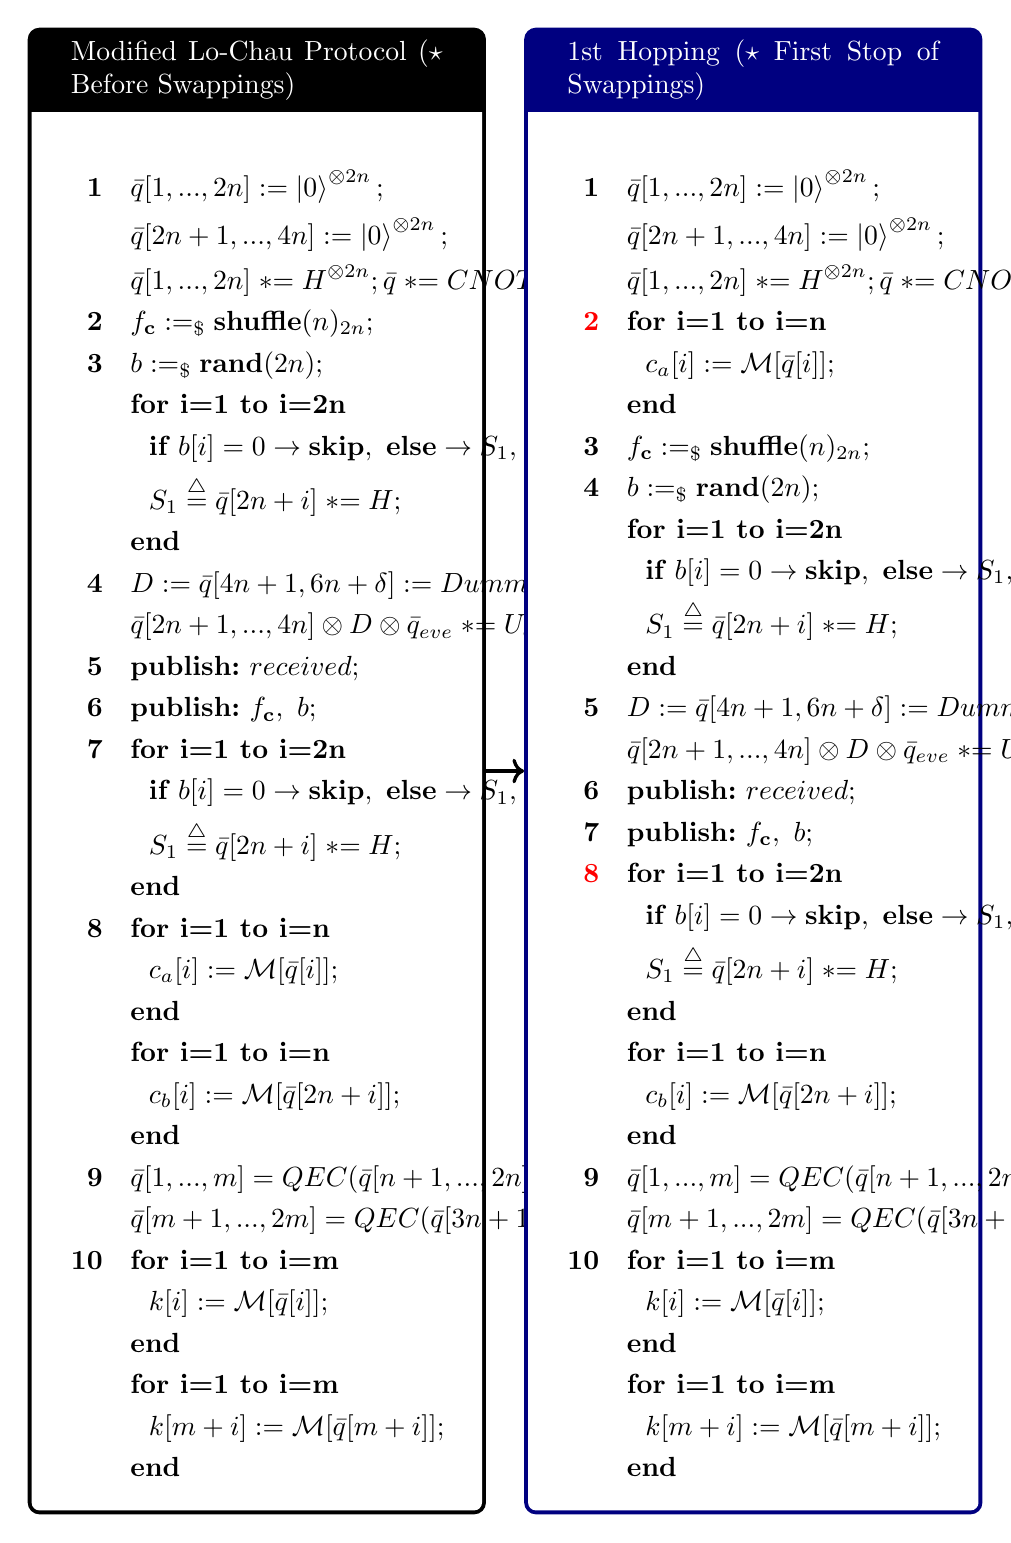
\begin{tikzpicture}[remember picture]
% Left box
\node[anchor=north west,inner sep=0pt,outer sep=0pt] (leftbox) at (0,0) {
\begin{minipage}[t]{0.48\textwidth}
\begin{tcolorbox}[colframe=black!75!black, colback=white, title=Modified Lo-Chau Protocol ($\star$ Before Swappings), width=\textwidth]
\begin{align*}
    \textbf{1} \quad & \bar{q}[1,...,2n] := \ket{0}^{\otimes 2n}; \\
    &\bar{q}[2n+1,...,4n] := \ket{0}^{\otimes 2n};\\
    \quad &\bar{q}[1,...,2n] \asteq H^{\otimes 2n}; \bar{q} \asteq CNOT; \\
    \textbf{2} \quad & f_{\textbf{c}}:=_\$\textbf{shuffle}(n)_{2n}; \\
    \textbf{3} \quad & b :=_\$ \textbf{rand}(2n); \\
    &\textbf{for~i=1~to~i=2n}\\
    &~~ \textbf{if }  b[i] = 0 \rightarrow \textbf{skip},~\textbf{else}\rightarrow S_{1},\\
    &~~ S_{1}\stackrel{\triangle}{=}\bar{q}[2n+i] \asteq H ;\\
    &\textbf{end}\\
    \textbf{4} \quad & {D}:= \bar{q}[4n+1,6n+\delta]:=Dummy;\\
    &\bar{q}[2n+1,...,4n]\otimes {D} \otimes \bar{q}_{eve} \asteq U_{\textbf{c}}(f_{\textbf{c}}); \\
    \textbf{5} \quad & \textbf{publish:}~ received;\\
    \textbf{6} \quad & \textbf{publish:}~ f_{\textbf{c}},~b;\\
    \textbf{7} \quad & \textbf{for~i=1~to~i=2n}\\
    &~~ \textbf{if }  b[i] = 0 \rightarrow \textbf{skip},~\textbf{else}\rightarrow S_{1} ,\\
    &~~ S_{1}\stackrel{\triangle}{=}\bar{q}[2n+i] \asteq H ;\\
    &\textbf{end}\\
    \textbf{8} \quad & \textbf{for~i=1~to~i=n}\\
    &~~ c_a[i]:= \mathcal{M} [\bar{q}[i]];\\
    &\textbf{end}\\
    \quad & \textbf{for~i=1~to~i=n}\\
    &~~ c_b[i]:= \mathcal{M} [\bar{q}[2n+i]];\\
    &\textbf{end}\\
    \textbf{9} \quad & \bar{q}[1,...,m]=QEC(\bar{q}[n+1,...,2n])\\
    \quad & \bar{q}[m+1,...,2m]=QEC(\bar{q}[3n+1,...,4n])\\
    \textbf{10} \quad & \textbf{for~i=1~to~i=m}\\
    &~~ k[i]:= \mathcal{M} [\bar{q}[i]];\\
    &\textbf{end}\\
    & \textbf{for~i=1~to~i=m}\\
    &~~ k[m+i]:= \mathcal{M} [\bar{q}[m+i]];\\
    &\textbf{end}
\end{align*}
\end{tcolorbox}
\end{minipage}
};

% Right box
\node[anchor=north west,inner sep=0pt,outer sep=0pt] (rightbox) at (0.52\textwidth,0) {
\begin{minipage}[t]{0.48\textwidth}
\begin{tcolorbox}[colframe=blue!50!black, colback=white, title=1st Hopping ($\star$ First Stop of Swappings), width=\textwidth]
\begin{align*}
    \textbf{1} \quad & \bar{q}[1,...,2n] := \ket{0}^{\otimes 2n}; \\
    &\bar{q}[2n+1,...,4n] := \ket{0}^{\otimes 2n};\\
    \quad &\bar{q}[1,...,2n] \asteq H^{\otimes 2n}; \bar{q} \asteq CNOT; \\
    \textbf{\textcolor{red}{2}} \quad & \textbf{for~i=1~to~i=n}\\
    &~~ c_a[i]:= \mathcal{M} [\bar{q}[i]];\\
    &\textbf{end}\\
    \textbf{{3}} \quad & f_{\textbf{c}}:=_\$\textbf{shuffle}(n)_{2n}; \\
    \textbf{{4}} \quad & b :=_\$ \textbf{rand}(2n); \\
    &\textbf{for~i=1~to~i=2n}\\
    &~~ \textbf{if }  b[i] = 0 \rightarrow \textbf{skip},~\textbf{else}\rightarrow S_{1} ,\\
    &~~ S_{1}\stackrel{\triangle}{=}\bar{q}[2n+i] \asteq H ;\\
    &\textbf{end}\\
    \textbf{{5}} \quad & {D}:= \bar{q}[4n+1,6n+\delta]:=Dummy;\\     &\bar{q}[2n+1,...,4n]\otimes {D} \otimes \bar{q}_{eve} \asteq U_{\textbf{c}}(f_{\textbf{c}}); \\
    \textbf{{6}} \quad & \textbf{publish:}~ received;\\
    \textbf{{7}} \quad & \textbf{publish:}~ f_{\textbf{c}},~b;\\
    \textbf{\textcolor{red}{8}} \quad & \textbf{for~i=1~to~i=2n}\\
    &~~ \textbf{if }  b[i] = 0 \rightarrow \textbf{skip},~\textbf{else}\rightarrow S_{1} ,\\
    &~~ S_{1}\stackrel{\triangle}{=}\bar{q}[2n+i] \asteq H ;\\
    &\textbf{end}\\
    \quad & \textbf{for~i=1~to~i=n}\\
    &~~ c_b[i]:= \mathcal{M} [\bar{q}[2n+i]];\\
    &\textbf{end}\\
    \textbf{9} \quad & \bar{q}[1,...,m]=QEC(\bar{q}[n+1,...,2n])\\
    \quad & \bar{q}[m+1,...,2m]=QEC(\bar{q}[3n+1,...,4n])\\
    \textbf{10} \quad & \textbf{for~i=1~to~i=m}\\
    &~~ k[i]:= \mathcal{M} [\bar{q}[i]];\\
    &\textbf{end}
    \\
    & \textbf{for~i=1~to~i=m}\\
    &~~ k[m+i]:= \mathcal{M} [\bar{q}[m+i]];\\
    &\textbf{end}
\end{align*}
\end{tcolorbox}
\end{minipage}
};

% Draw arrow between boxes
\draw[->, very thick] (leftbox.east) -- node[above]{} (rightbox.west);

\end{tikzpicture}
\newpage

\noindent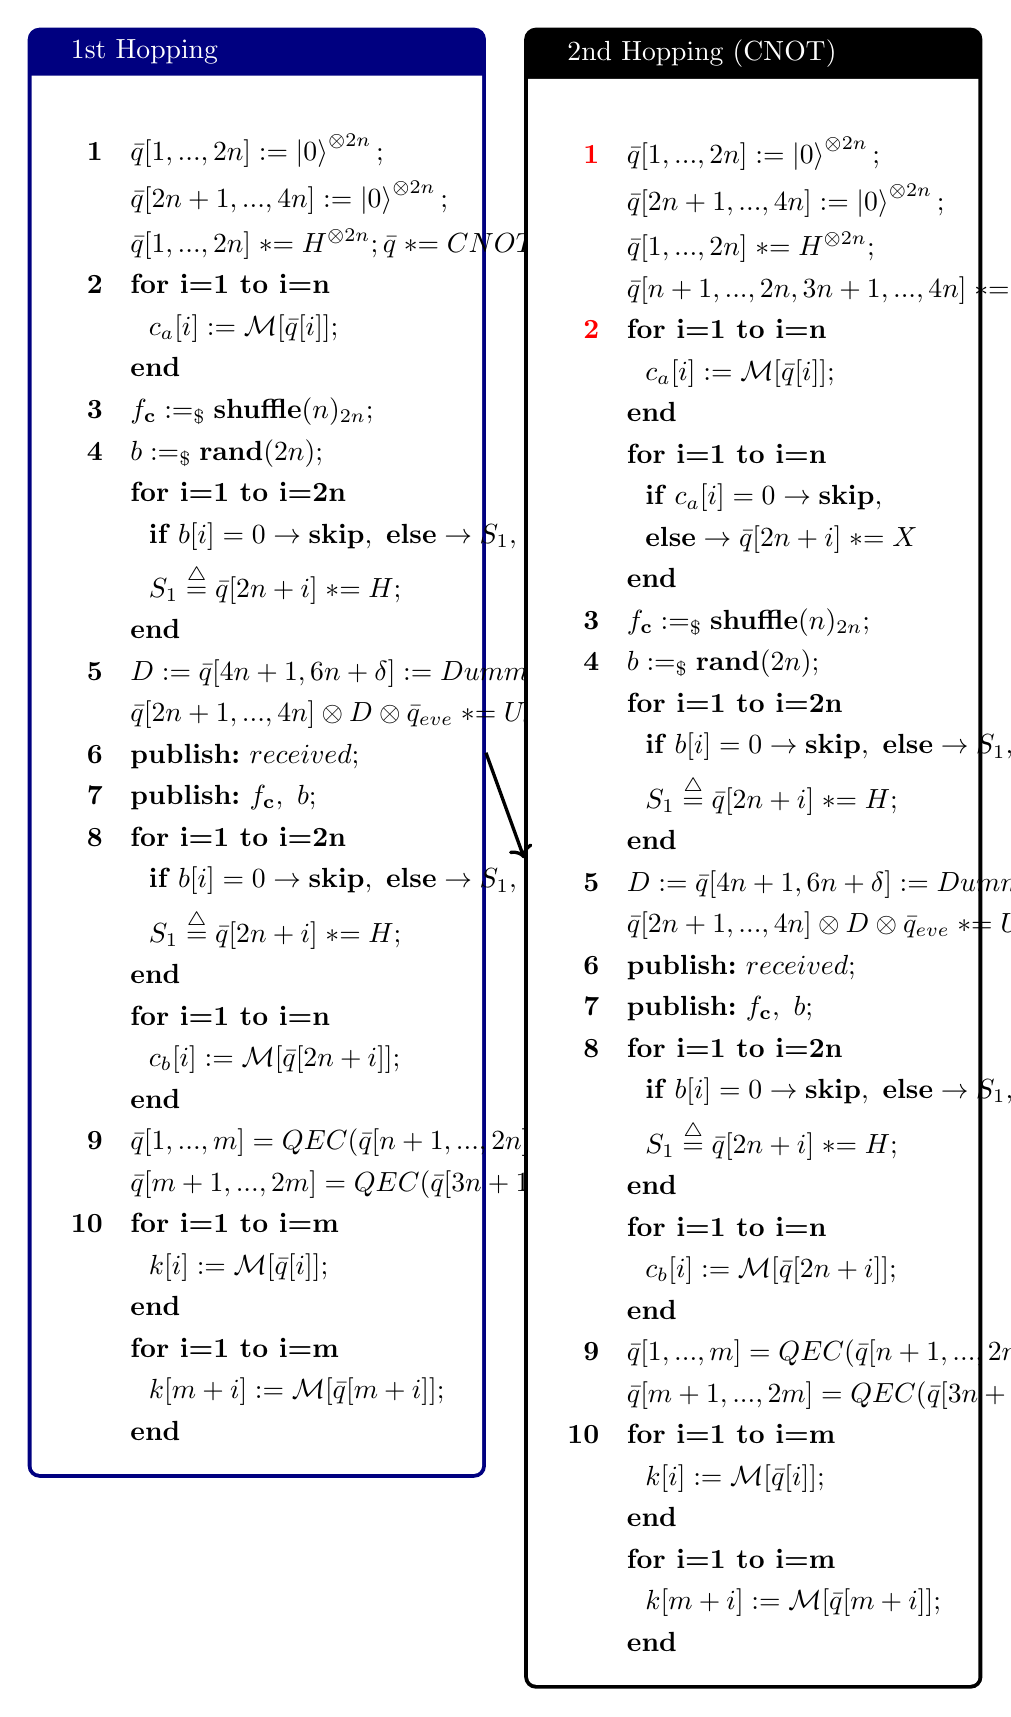
\begin{tikzpicture}[remember picture]

% Left box
\node[anchor=north west,inner sep=0pt,outer sep=0pt] (leftbox) at (0,0) {
\begin{minipage}[t]{0.48\textwidth}
\begin{tcolorbox}[colframe=blue!50!black, colback=white, title=1st Hopping, width=\textwidth]
\begin{align*}
    \textbf{1} \quad & \bar{q}[1,...,2n] := \ket{0}^{\otimes 2n}; \\
    &\bar{q}[2n+1,...,4n] := \ket{0}^{\otimes 2n};\\
    \quad &\bar{q}[1,...,2n] \asteq H^{\otimes 2n}; \bar{q} \asteq CNOT; \\
    \textbf{{2}} \quad & \textbf{for~i=1~to~i=n}\\
    &~~ c_a[i]:= \mathcal{M} [\bar{q}[i]];\\
    &\textbf{end}\\
    \textbf{{3}} \quad & f_{\textbf{c}}:=_\$\textbf{shuffle}(n)_{2n}; \\
    \textbf{{4}} \quad & b :=_\$ \textbf{rand}(2n); \\
    &\textbf{for~i=1~to~i=2n}\\
    &~~ \textbf{if }  b[i] = 0 \rightarrow \textbf{skip},~\textbf{else}\rightarrow S_{1} ,\\
    &~~ S_{1}\stackrel{\triangle}{=}\bar{q}[2n+i] \asteq H ;\\
    &\textbf{end}\\
    \textbf{{5}} \quad & {D}:= \bar{q}[4n+1,6n+\delta]:=Dummy;\\     &\bar{q}[2n+1,...,4n]\otimes {D} \otimes \bar{q}_{eve} \asteq U_{\textbf{c}}(f_{\textbf{c}}); \\
    \textbf{{6}} \quad & \textbf{publish:}~ received;\\
    \textbf{{7}} \quad & \textbf{publish:}~ f_{\textbf{c}},~b;\\
    \textbf{{8}} \quad & \textbf{for~i=1~to~i=2n}\\
    &~~ \textbf{if }  b[i] = 0 \rightarrow \textbf{skip},~\textbf{else}\rightarrow S_{1} ,\\
    &~~ S_{1}\stackrel{\triangle}{=}\bar{q}[2n+i] \asteq H ;\\
    &\textbf{end}\\
    \quad & \textbf{for~i=1~to~i=n}\\
    &~~ c_b[i]:= \mathcal{M} [\bar{q}[2n+i]];\\
    &\textbf{end}\\
    \textbf{9} \quad & \bar{q}[1,...,m]=QEC(\bar{q}[n+1,...,2n])\\
    \quad & \bar{q}[m+1,...,2m]=QEC(\bar{q}[3n+1,...,4n])\\
    \textbf{10} \quad & \textbf{for~i=1~to~i=m}\\
    &~~ k[i]:= \mathcal{M} [\bar{q}[i]];\\
    &\textbf{end}
    \\
    & \textbf{for~i=1~to~i=m}\\
    &~~ k[m+i]:= \mathcal{M} [\bar{q}[m+i]];\\
    &\textbf{end}
\end{align*}
\end{tcolorbox}
\end{minipage}
};

% Right box
\node[anchor=north west,inner sep=0pt,outer sep=0pt] (rightbox) at (0.52\textwidth,0) {
\begin{minipage}[t]{0.48\textwidth}
\begin{tcolorbox}[colframe=black!50!black, colback=white, title=2nd Hopping (CNOT), width=\textwidth]
\begin{align*}
    \textbf{\textcolor{red}{1}} \quad & \bar{q}[1,...,2n] := \ket{0}^{\otimes 2n}; \\
    &\bar{q}[2n+1,...,4n] := \ket{0}^{\otimes 2n};\\
    \quad &\bar{q}[1,...,2n] \asteq H^{\otimes 2n}; \\
    &\bar{q}[n+1,...,2n,3n+1,...,4n] \asteq CNOT; \\
    \textbf{\textcolor{red}{2}} \quad & \textbf{for~i=1~to~i=n}\\
    &~~ c_a[i]:= \mathcal{M} [\bar{q}[i]];\\
    &\textbf{end}\\
    &\textbf{for~i=1~to~i=n}\\
    &~~ \textbf{if }  c_a[i]=0\rightarrow \textbf{skip},\\ &~~\textbf{else}   \rightarrow \bar{q}[2n+i]\asteq X\\
    &\textbf{end}\ \\
    \textbf{{3}} \quad & f_{\textbf{c}}:=_\$\textbf{shuffle}(n)_{2n}; \\
    \textbf{{4}} \quad & b :=_\$ \textbf{rand}(2n); \\
    &\textbf{for~i=1~to~i=2n}\\
    &~~ \textbf{if }  b[i] = 0 \rightarrow \textbf{skip},~\textbf{else}\rightarrow S_{1} ,\\
    &~~ S_{1}\stackrel{\triangle}{=}\bar{q}[2n+i] \asteq H ;\\
    &\textbf{end}\\
    \textbf{{5}} \quad & {D}:= \bar{q}[4n+1,6n+\delta]:=Dummy;\\     &\bar{q}[2n+1,...,4n]\otimes {D} \otimes \bar{q}_{eve} \asteq U_{\textbf{c}}(f_{\textbf{c}}); \\
    \textbf{{6}} \quad & \textbf{publish:}~ received;\\
    \textbf{{7}} \quad & \textbf{publish:}~ f_{\textbf{c}},~b;\\
    \textbf{{8}} \quad & \textbf{for~i=1~to~i=2n}\\
    &~~ \textbf{if }  b[i] = 0 \rightarrow \textbf{skip},~\textbf{else}\rightarrow S_{1} ,\\
    &~~ S_{1}\stackrel{\triangle}{=}\bar{q}[2n+i] \asteq H ;\\
    &\textbf{end}\\
    \quad & \textbf{for~i=1~to~i=n}\\
    &~~ c_b[i]:= \mathcal{M} [\bar{q}[2n+i]];\\
    &\textbf{end}\\
    \textbf{9} \quad & \bar{q}[1,...,m]=QEC(\bar{q}[n+1,...,2n])\\
    \quad & \bar{q}[m+1,...,2m]=QEC(\bar{q}[3n+1,...,4n])\\
    \textbf{10} \quad & \textbf{for~i=1~to~i=m}\\
    &~~ k[i]:= \mathcal{M} [\bar{q}[i]];\\
    &\textbf{end}
    \\
    & \textbf{for~i=1~to~i=m}\\
    &~~ k[m+i]:= \mathcal{M} [\bar{q}[m+i]];\\
    &\textbf{end}
\end{align*}
\end{tcolorbox}
\end{minipage}
};

% Draw arrow between boxes
\draw[->, very thick] (leftbox.east) -- node[above]{} (rightbox.west);

\end{tikzpicture}
\newpage

\noindent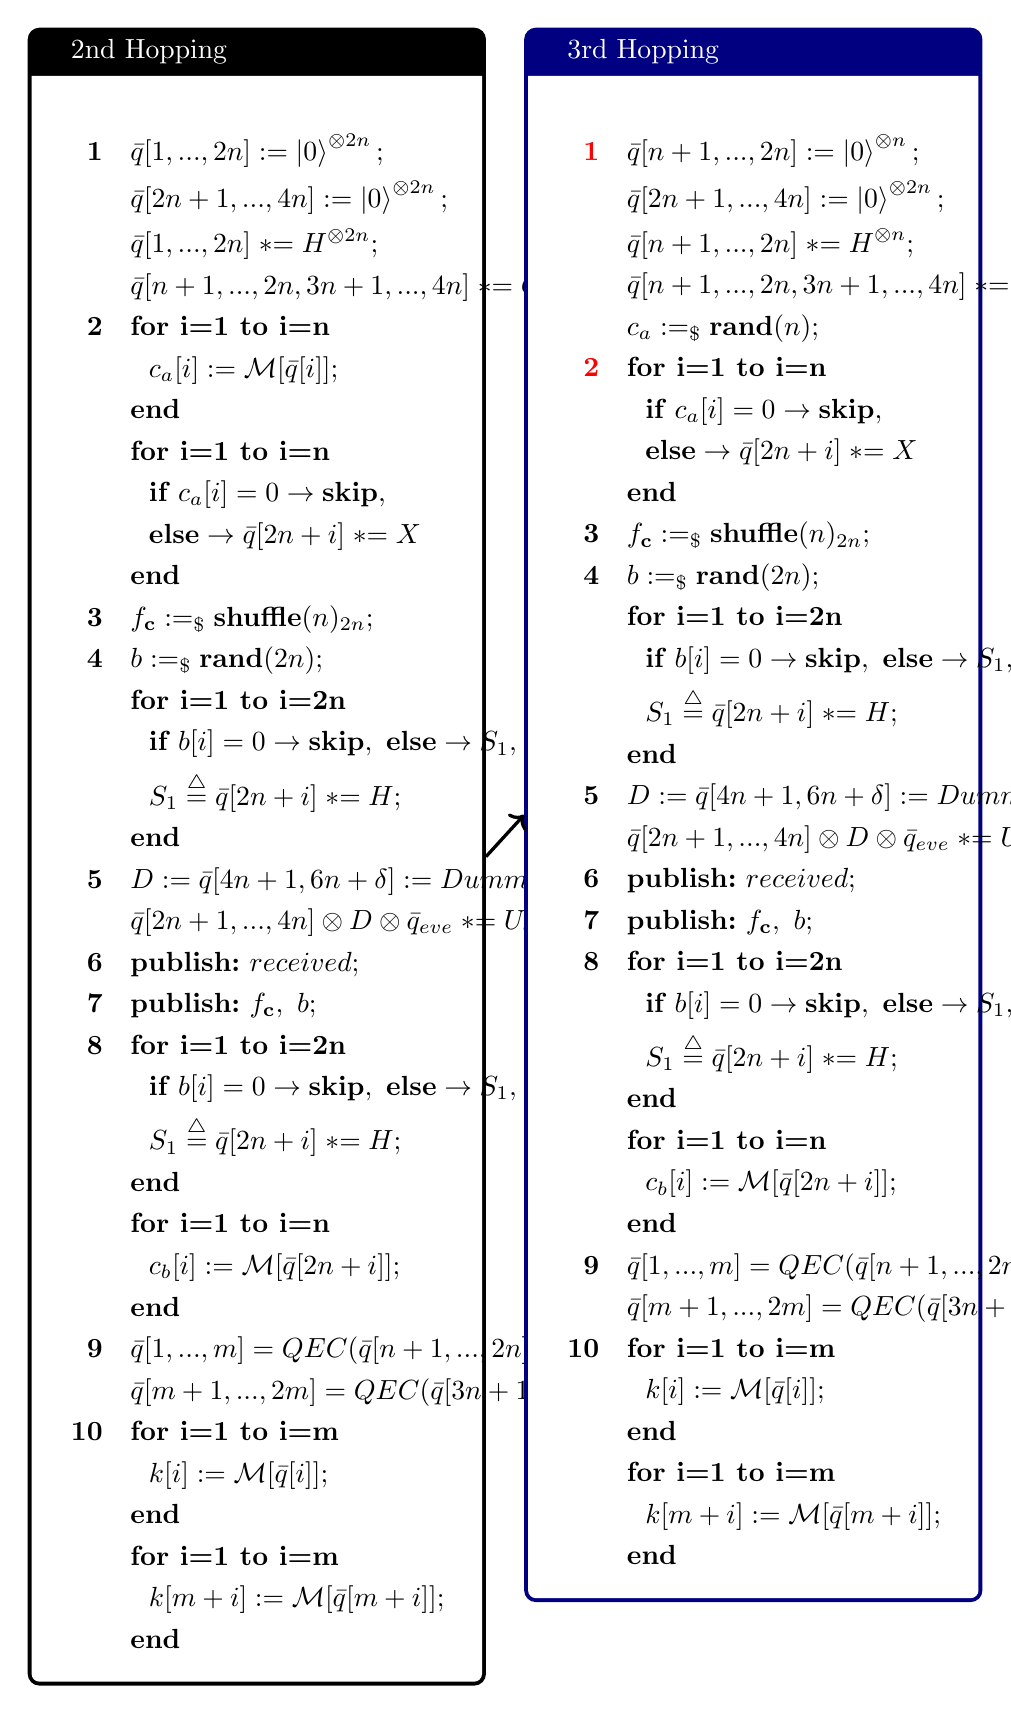
\begin{tikzpicture}[remember picture]

% Left box
\node[anchor=north west,inner sep=0pt,outer sep=0pt] (leftbox) at (0,0) {
\begin{minipage}[t]{0.48\textwidth}
\begin{tcolorbox}[colframe=black!75!black, colback=white, title=2nd Hopping, width=\textwidth]
\begin{align*}
    \textbf{{1}} \quad & \bar{q}[1,...,2n] := \ket{0}^{\otimes 2n}; \\
    &\bar{q}[2n+1,...,4n] := \ket{0}^{\otimes 2n};\\
    \quad &\bar{q}[1,...,2n] \asteq H^{\otimes 2n}; \\
    &\bar{q}[n+1,...,2n,3n+1,...,4n] \asteq CNOT; \\
    \textbf{{2}} \quad &  \textbf{for~i=1~to~i=n}\\
    &~~ c_a[i]:= \mathcal{M} [\bar{q}[i]];\\
    &\textbf{end}\\
    &\textbf{for~i=1~to~i=n}\\
    &~~ \textbf{if }  c_a[i]=0\rightarrow \textbf{skip},\\ &~~\textbf{else}   \rightarrow \bar{q}[2n+i]\asteq X\\
    &\textbf{end}\ \\
    \textbf{{3}} \quad & f_{\textbf{c}}:=_\$\textbf{shuffle}(n)_{2n}; \\
    \textbf{{4}} \quad & b :=_\$ \textbf{rand}(2n); \\
    &\textbf{for~i=1~to~i=2n}\\
    &~~ \textbf{if }  b[i] = 0 \rightarrow \textbf{skip},~\textbf{else}\rightarrow S_{1} ,\\
    &~~ S_{1}\stackrel{\triangle}{=}\bar{q}[2n+i] \asteq H ;\\
    &\textbf{end}\\
    \textbf{{5}} \quad & {D}:= \bar{q}[4n+1,6n+\delta]:=Dummy;\\     &\bar{q}[2n+1,...,4n]\otimes {D} \otimes \bar{q}_{eve} \asteq U_{\textbf{c}}(f_{\textbf{c}}); \\
    \textbf{{6}} \quad & \textbf{publish:}~ received;\\
    \textbf{{7}} \quad & \textbf{publish:}~ f_{\textbf{c}},~b;\\
    \textbf{{8}} \quad & \textbf{for~i=1~to~i=2n}\\
    &~~ \textbf{if }  b[i] = 0 \rightarrow \textbf{skip},~\textbf{else}\rightarrow S_{1} ,\\
    &~~ S_{1}\stackrel{\triangle}{=}\bar{q}[2n+i] \asteq H ;\\
    &\textbf{end}\\
    \quad & \textbf{for~i=1~to~i=n}\\
    &~~ c_b[i]:= \mathcal{M} [\bar{q}[2n+i]];\\
    &\textbf{end}\\
    \textbf{9} \quad & \bar{q}[1,...,m]=QEC(\bar{q}[n+1,...,2n])\\
    \quad & \bar{q}[m+1,...,2m]=QEC(\bar{q}[3n+1,...,4n])\\
    \textbf{10} \quad & \textbf{for~i=1~to~i=m}\\
    &~~ k[i]:= \mathcal{M} [\bar{q}[i]];\\
    &\textbf{end}
    \\
    & \textbf{for~i=1~to~i=m}\\
    &~~ k[m+i]:= \mathcal{M} [\bar{q}[m+i]];\\
    &\textbf{end}
\end{align*}
\end{tcolorbox}
\end{minipage}
};

% Right box
\node[anchor=north west,inner sep=0pt,outer sep=0pt] (rightbox) at (0.52\textwidth,0) {
\begin{minipage}[t]{0.48\textwidth}
\begin{tcolorbox}[colframe=blue!50!black, colback=white, title=3rd Hopping, width=\textwidth]
\begin{align*}
    \textbf{\textcolor{red}{1}} \quad &\bar{q}[n+1,...,2n] := \ket{0}^{\otimes n};\\
    &\bar{q}[2n+1,...,4n] := \ket{0}^{\otimes 2n};\\
    \quad &\bar{q}[n+1,...,2n] \asteq H^{\otimes n}; \\
    &\bar{q}[n+1,...,2n,3n+1,...,4n] \asteq CNOT; \\
    & c_a :=_\$ \textbf{rand}(n); \\ \textbf{\textcolor{red}{2}} \quad &\textbf{for~i=1~to~i=n}\\
    &~~ \textbf{if }  c_a[i] = 0 \rightarrow \textbf{skip},\\ &~~\textbf{else}   \rightarrow \bar{q}[2n+i]\asteq X\\
    &\textbf{end}\ \\
    \textbf{{3}} \quad & f_{\textbf{c}}:=_\$\textbf{shuffle}(n)_{2n}; \\
    \textbf{{4}} \quad & b :=_\$ \textbf{rand}(2n); \\
    &\textbf{for~i=1~to~i=2n}\\
    &~~ \textbf{if }  b[i] = 0 \rightarrow \textbf{skip},~\textbf{else}\rightarrow S_{1} ,\\
    &~~ S_{1}\stackrel{\triangle}{=}\bar{q}[2n+i] \asteq H ;\\
    &\textbf{end}\\
    \textbf{{5}} \quad & {D}:= \bar{q}[4n+1,6n+\delta]:=Dummy;\\     &\bar{q}[2n+1,...,4n]\otimes {D} \otimes \bar{q}_{eve} \asteq U_{\textbf{c}}(f_{\textbf{c}}); \\
    \textbf{{6}} \quad & \textbf{publish:}~ received;\\
    \textbf{{7}} \quad & \textbf{publish:}~ f_{\textbf{c}},~b;\\
    \textbf{{8}} \quad & \textbf{for~i=1~to~i=2n}\\
    &~~ \textbf{if }  b[i] = 0 \rightarrow \textbf{skip},~\textbf{else}\rightarrow S_{1} ,\\
    &~~ S_{1}\stackrel{\triangle}{=}\bar{q}[2n+i] \asteq H ;\\
    &\textbf{end}\\
    \quad & \textbf{for~i=1~to~i=n}\\
    &~~ c_b[i]:= \mathcal{M} [\bar{q}[2n+i]];\\
    &\textbf{end}\\
    \textbf{9} \quad & \bar{q}[1,...,m]=QEC(\bar{q}[n+1,...,2n])\\
    \quad & \bar{q}[m+1,...,2m]=QEC(\bar{q}[3n+1,...,4n])\\
    \textbf{10} \quad & \textbf{for~i=1~to~i=m}\\
    &~~ k[i]:= \mathcal{M} [\bar{q}[i]];\\
    &\textbf{end}
    \\
    & \textbf{for~i=1~to~i=m}\\
    &~~ k[m+i]:= \mathcal{M} [\bar{q}[m+i]];\\
    &\textbf{end}
\end{align*}
\end{tcolorbox}
\end{minipage}
};

% Draw arrow between boxes
\draw[->, very thick] (leftbox.east) -- node[above]{} (rightbox.west);

\end{tikzpicture}
\newpage

\noindent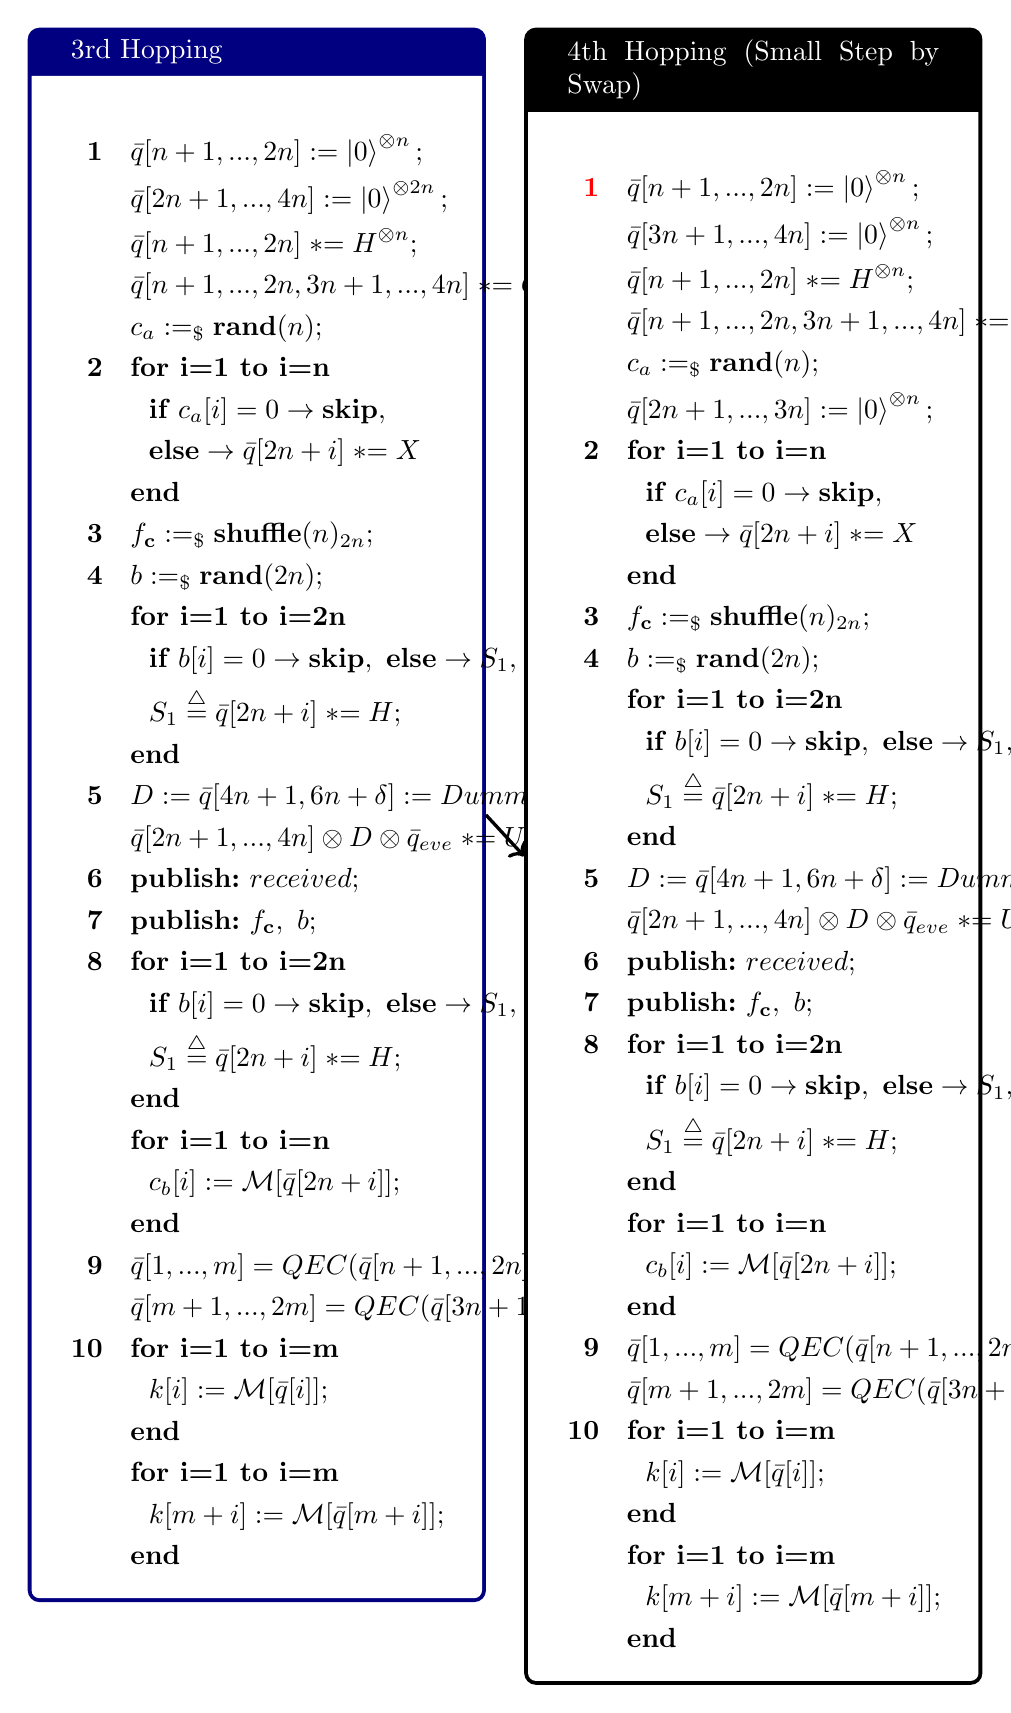
\begin{tikzpicture}[remember picture]

% Left box
\node[anchor=north west,inner sep=0pt,outer sep=0pt] (leftbox) at (0,0) {
\begin{minipage}[t]{0.48\textwidth}
\begin{tcolorbox}[colframe=blue!50!black, colback=white, title=3rd Hopping, width=\textwidth]
\begin{align*}
    \textbf{{1}} \quad &\bar{q}[n+1,...,2n] := \ket{0}^{\otimes n};\\
    &\bar{q}[2n+1,...,4n] := \ket{0}^{\otimes 2n};\\
    \quad &\bar{q}[n+1,...,2n] \asteq H^{\otimes n}; \\
    &\bar{q}[n+1,...,2n,3n+1,...,4n] \asteq CNOT; \\
    & c_a :=_\$ \textbf{rand}(n); \\ 
    \textbf{{2}} \quad &\textbf{for~i=1~to~i=n}\\
    &~~ \textbf{if }  c_a[i] = 0 \rightarrow \textbf{skip},\\ &~~\textbf{else}   \rightarrow \bar{q}[2n+i]\asteq X\\
    &\textbf{end}\ \\
    \textbf{{3}} \quad & f_{\textbf{c}}:=_\$\textbf{shuffle}(n)_{2n}; \\
    \textbf{{4}} \quad & b :=_\$ \textbf{rand}(2n); \\
    &\textbf{for~i=1~to~i=2n}\\
    &~~ \textbf{if }  b[i] = 0 \rightarrow \textbf{skip},~\textbf{else}\rightarrow S_{1} ,\\
    &~~ S_{1}\stackrel{\triangle}{=}\bar{q}[2n+i] \asteq H ;\\
    &\textbf{end}\\
    \textbf{{5}} \quad & {D}:= \bar{q}[4n+1,6n+\delta]:=Dummy;\\     &\bar{q}[2n+1,...,4n]\otimes {D} \otimes \bar{q}_{eve} \asteq U_{\textbf{c}}(f_{\textbf{c}}); \\
    \textbf{{6}} \quad & \textbf{publish:}~ received;\\
    \textbf{{7}} \quad & \textbf{publish:}~ f_{\textbf{c}},~b;\\
    \textbf{{8}} \quad & \textbf{for~i=1~to~i=2n}\\
    &~~ \textbf{if }  b[i] = 0 \rightarrow \textbf{skip},~\textbf{else}\rightarrow S_{1} ,\\
    &~~ S_{1}\stackrel{\triangle}{=}\bar{q}[2n+i] \asteq H ;\\
    &\textbf{end}\\
    \quad & \textbf{for~i=1~to~i=n}\\
    &~~ c_b[i]:= \mathcal{M} [\bar{q}[2n+i]];\\
    &\textbf{end}\\
    \textbf{9} \quad & \bar{q}[1,...,m]=QEC(\bar{q}[n+1,...,2n])\\
    \quad & \bar{q}[m+1,...,2m]=QEC(\bar{q}[3n+1,...,4n])\\
    \textbf{10} \quad & \textbf{for~i=1~to~i=m}\\
    &~~ k[i]:= \mathcal{M} [\bar{q}[i]];\\
    &\textbf{end}
    \\
    & \textbf{for~i=1~to~i=m}\\
    &~~ k[m+i]:= \mathcal{M} [\bar{q}[m+i]];\\
    &\textbf{end}
\end{align*}
\end{tcolorbox}
\end{minipage}
};

% Right box
\node[anchor=north west,inner sep=0pt,outer sep=0pt] (rightbox) at (0.52\textwidth,0) {
\begin{minipage}[t]{0.48\textwidth}
\begin{tcolorbox}[colframe=black!50!black, colback=white, title=4th Hopping (Small Step by Swap), width=\textwidth]
\begin{align*}
    \textbf{\textcolor{red}{1}} \quad &\bar{q}[n+1,...,2n] := \ket{0}^{\otimes n};\\
    &\bar{q}[3n+1,...,4n] := \ket{0}^{\otimes n};\\
    \quad &\bar{q}[n+1,...,2n] \asteq H^{\otimes n}; \\
    &\bar{q}[n+1,...,2n,3n+1,...,4n] \asteq CNOT; \\
    & c_a :=_\$ \textbf{rand}(n); \\ 
    &\bar{q}[2n+1,...,3n] := \ket{0}^{\otimes n};\\
    \textbf{{2}} \quad &\textbf{for~i=1~to~i=n}\\
    &~~ \textbf{if }  c_a[i] = 0 \rightarrow \textbf{skip},\\ &~~\textbf{else}   \rightarrow \bar{q}[2n+i]\asteq X\\
    &\textbf{end}\ \\
    \textbf{{3}} \quad & f_{\textbf{c}}:=_\$\textbf{shuffle}(n)_{2n}; \\
    \textbf{{4}} \quad & b :=_\$ \textbf{rand}(2n); \\
    &\textbf{for~i=1~to~i=2n}\\
    &~~ \textbf{if }  b[i] = 0 \rightarrow \textbf{skip},~\textbf{else}\rightarrow S_{1} ,\\
    &~~ S_{1}\stackrel{\triangle}{=}\bar{q}[2n+i] \asteq H ;\\
    &\textbf{end}\\
    \textbf{{5}} \quad & {D}:= \bar{q}[4n+1,6n+\delta]:=Dummy;\\     &\bar{q}[2n+1,...,4n]\otimes {D} \otimes \bar{q}_{eve} \asteq U_{\textbf{c}}(f_{\textbf{c}}); \\
    \textbf{{6}} \quad & \textbf{publish:}~ received;\\
    \textbf{{7}} \quad & \textbf{publish:}~ f_{\textbf{c}},~b;\\
    \textbf{{8}} \quad & \textbf{for~i=1~to~i=2n}\\
    &~~ \textbf{if }  b[i] = 0 \rightarrow \textbf{skip},~\textbf{else}\rightarrow S_{1} ,\\
    &~~ S_{1}\stackrel{\triangle}{=}\bar{q}[2n+i] \asteq H ;\\
    &\textbf{end}\\
    \quad & \textbf{for~i=1~to~i=n}\\
    &~~ c_b[i]:= \mathcal{M} [\bar{q}[2n+i]];\\
    &\textbf{end}\\
    \textbf{9} \quad & \bar{q}[1,...,m]=QEC(\bar{q}[n+1,...,2n])\\
    \quad & \bar{q}[m+1,...,2m]=QEC(\bar{q}[3n+1,...,4n])\\
    \textbf{10} \quad & \textbf{for~i=1~to~i=m}\\
    &~~ k[i]:= \mathcal{M} [\bar{q}[i]];\\
    &\textbf{end}
    \\
    & \textbf{for~i=1~to~i=m}\\
    &~~ k[m+i]:= \mathcal{M} [\bar{q}[m+i]];\\
    &\textbf{end}
\end{align*}
\end{tcolorbox}
\end{minipage}
};

% Draw arrow between boxes
\draw[->, very thick] (leftbox.east) -- node[above]{} (rightbox.west);

\end{tikzpicture}
\newpage

\noindent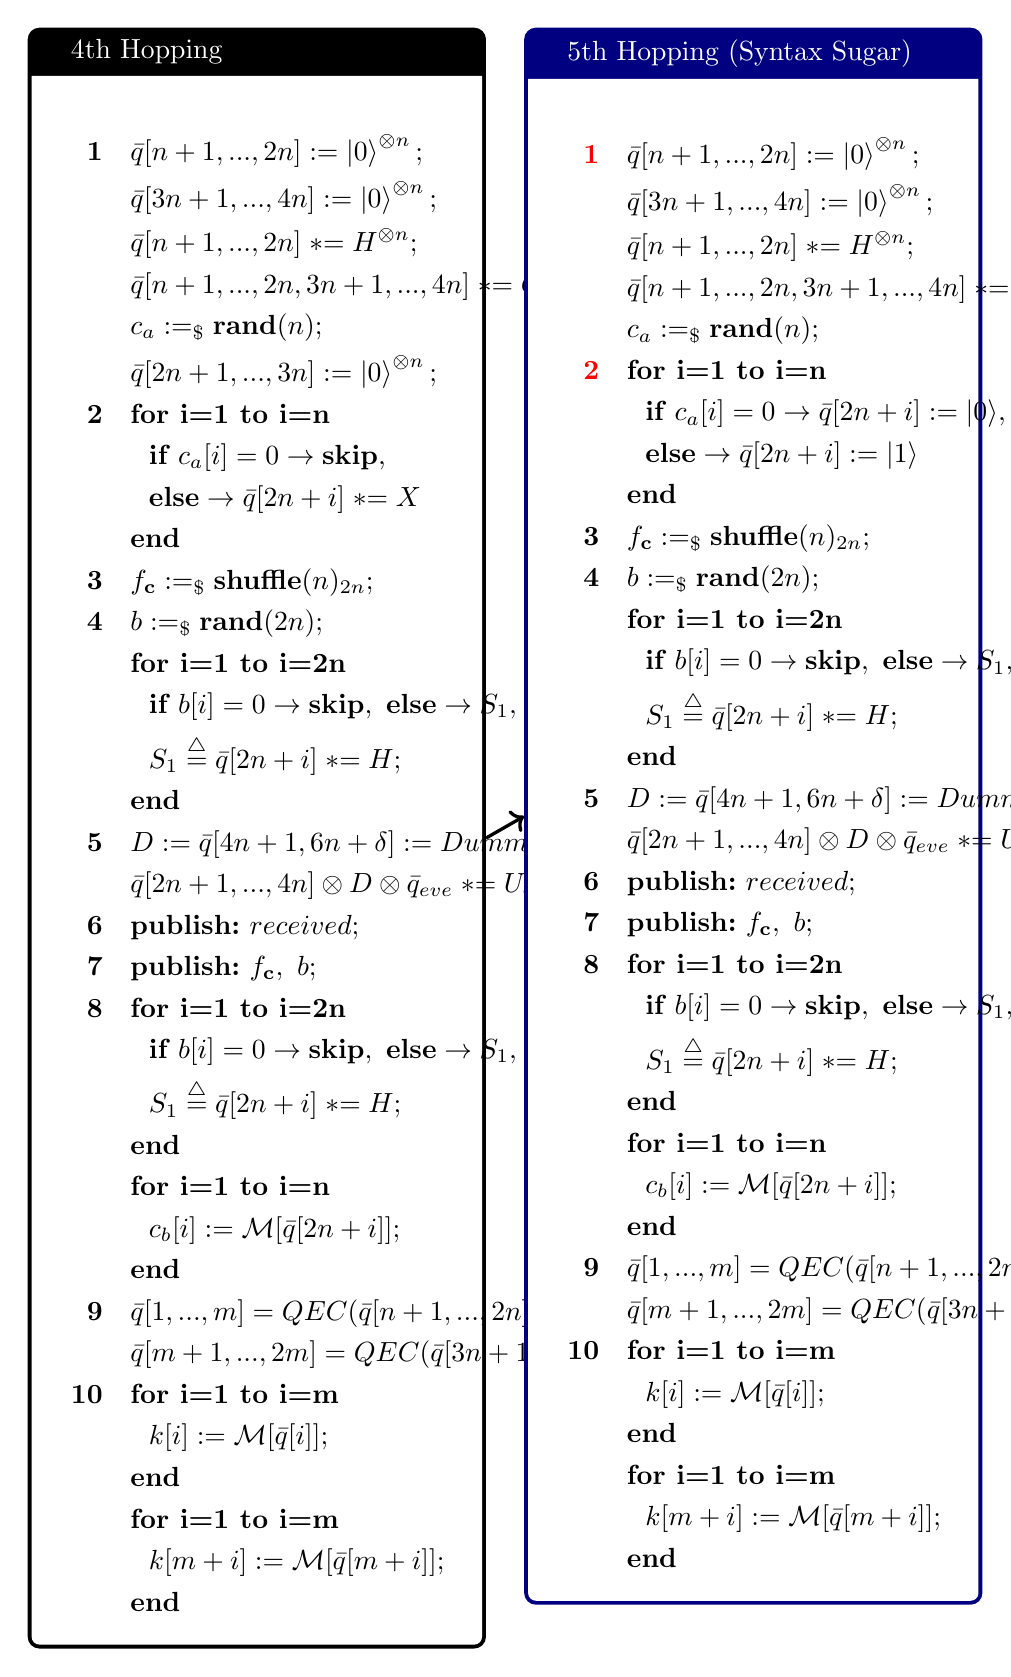
\begin{tikzpicture}[remember picture]

% Left box
\node[anchor=north west,inner sep=0pt,outer sep=0pt] (leftbox) at (0,0) {
\begin{minipage}[t]{0.48\textwidth}
\begin{tcolorbox}[colframe=black!75!black, colback=white, title=4th Hopping, width=\textwidth]
\begin{align*}
    \textbf{{1}} \quad &\bar{q}[n+1,...,2n] := \ket{0}^{\otimes n};\\
    &\bar{q}[3n+1,...,4n] := \ket{0}^{\otimes n};\\
    \quad &\bar{q}[n+1,...,2n] \asteq H^{\otimes n}; \\
    &\bar{q}[n+1,...,2n,3n+1,...,4n] \asteq CNOT; \\
    & c_a :=_\$ \textbf{rand}(n); \\ 
    &\bar{q}[2n+1,...,3n] := \ket{0}^{\otimes n};\\
    \textbf{{2}} \quad &\textbf{for~i=1~to~i=n}\\
    &~~ \textbf{if }  c_a[i] = 0 \rightarrow \textbf{skip},\\ &~~\textbf{else}   \rightarrow \bar{q}[2n+i]\asteq X\\
    &\textbf{end}\ \\
    \textbf{{3}} \quad & f_{\textbf{c}}:=_\$\textbf{shuffle}(n)_{2n}; \\
    \textbf{{4}} \quad & b :=_\$ \textbf{rand}(2n); \\
    &\textbf{for~i=1~to~i=2n}\\
    &~~ \textbf{if }  b[i] = 0 \rightarrow \textbf{skip},~\textbf{else}\rightarrow S_{1} ,\\
    &~~ S_{1}\stackrel{\triangle}{=}\bar{q}[2n+i] \asteq H ;\\
    &\textbf{end}\\
    \textbf{{5}} \quad & {D}:= \bar{q}[4n+1,6n+\delta]:=Dummy;\\     &\bar{q}[2n+1,...,4n]\otimes {D} \otimes \bar{q}_{eve} \asteq U_{\textbf{c}}(f_{\textbf{c}}); \\
    \textbf{{6}} \quad & \textbf{publish:}~ received;\\
    \textbf{{7}} \quad & \textbf{publish:}~ f_{\textbf{c}},~b;\\
    \textbf{{8}} \quad & \textbf{for~i=1~to~i=2n}\\
    &~~ \textbf{if }  b[i] = 0 \rightarrow \textbf{skip},~\textbf{else}\rightarrow S_{1} ,\\
    &~~ S_{1}\stackrel{\triangle}{=}\bar{q}[2n+i] \asteq H ;\\
    &\textbf{end}\\
    \quad & \textbf{for~i=1~to~i=n}\\
    &~~ c_b[i]:= \mathcal{M} [\bar{q}[2n+i]];\\
    &\textbf{end}\\
    \textbf{9} \quad & \bar{q}[1,...,m]=QEC(\bar{q}[n+1,...,2n])\\
    \quad & \bar{q}[m+1,...,2m]=QEC(\bar{q}[3n+1,...,4n])\\
    \textbf{10} \quad & \textbf{for~i=1~to~i=m}\\
    &~~ k[i]:= \mathcal{M} [\bar{q}[i]];\\
    &\textbf{end}
    \\
    & \textbf{for~i=1~to~i=m}\\
    &~~ k[m+i]:= \mathcal{M} [\bar{q}[m+i]];\\
    &\textbf{end}
\end{align*}
\end{tcolorbox}
\end{minipage}
};

% Right box
\node[anchor=north west,inner sep=0pt,outer sep=0pt] (rightbox) at (0.52\textwidth,0) {
\begin{minipage}[t]{0.48\textwidth}
\begin{tcolorbox}[colframe=blue!50!black, colback=white, title=5th Hopping (Syntax Sugar), width=\textwidth]
\begin{align*}
    \textbf{\textcolor{red}{1}} \quad &\bar{q}[n+1,...,2n] := \ket{0}^{\otimes n};\\
    &\bar{q}[3n+1,...,4n] := \ket{0}^{\otimes n};\\
    \quad &\bar{q}[n+1,...,2n] \asteq H^{\otimes n}; \\
    &\bar{q}[n+1,...,2n,3n+1,...,4n] \asteq CNOT; \\
    & c_a :=_\$ \textbf{rand}(n); \\ 
    \textbf{\textcolor{red}{2}} \quad &\textbf{for~i=1~to~i=n}\\
    &~~ \textbf{if }  c_a[i] = 0 \rightarrow \bar{q}[2n+i] := |0\rangle,\\ &~~\textbf{else}   \rightarrow \bar{q}[2n+i] := |1\rangle\\
    &\textbf{end}\ \\
    \textbf{{3}} \quad & f_{\textbf{c}}:=_\$\textbf{shuffle}(n)_{2n}; \\
    \textbf{{4}} \quad & b :=_\$ \textbf{rand}(2n); \\
    &\textbf{for~i=1~to~i=2n}\\
    &~~ \textbf{if }  b[i] = 0 \rightarrow \textbf{skip},~\textbf{else}\rightarrow S_{1} ,\\
    &~~ S_{1}\stackrel{\triangle}{=}\bar{q}[2n+i] \asteq H ;\\
    &\textbf{end}\\
    \textbf{{5}} \quad & {D}:= \bar{q}[4n+1,6n+\delta]:=Dummy;\\     &\bar{q}[2n+1,...,4n]\otimes {D} \otimes \bar{q}_{eve} \asteq U_{\textbf{c}}(f_{\textbf{c}}); \\
    \textbf{{6}} \quad & \textbf{publish:}~ received;\\
    \textbf{{7}} \quad & \textbf{publish:}~ f_{\textbf{c}},~b;\\
    \textbf{{8}} \quad & \textbf{for~i=1~to~i=2n}\\
    &~~ \textbf{if }  b[i] = 0 \rightarrow \textbf{skip},~\textbf{else}\rightarrow S_{1} ,\\
    &~~ S_{1}\stackrel{\triangle}{=}\bar{q}[2n+i] \asteq H ;\\
    &\textbf{end}\\
    \quad & \textbf{for~i=1~to~i=n}\\
    &~~ c_b[i]:= \mathcal{M} [\bar{q}[2n+i]];\\
    &\textbf{end}\\
    \textbf{9} \quad & \bar{q}[1,...,m]=QEC(\bar{q}[n+1,...,2n])\\
    \quad & \bar{q}[m+1,...,2m]=QEC(\bar{q}[3n+1,...,4n])\\
    \textbf{10} \quad & \textbf{for~i=1~to~i=m}\\
    &~~ k[i]:= \mathcal{M} [\bar{q}[i]];\\
    &\textbf{end}
    \\
    & \textbf{for~i=1~to~i=m}\\
    &~~ k[m+i]:= \mathcal{M} [\bar{q}[m+i]];\\
    &\textbf{end}
\end{align*}
\end{tcolorbox}
\end{minipage}
};

% Draw arrow between boxes
\draw[->, very thick] (leftbox.east) -- node[above]{} (rightbox.west);

\end{tikzpicture}
\newpage

\noindent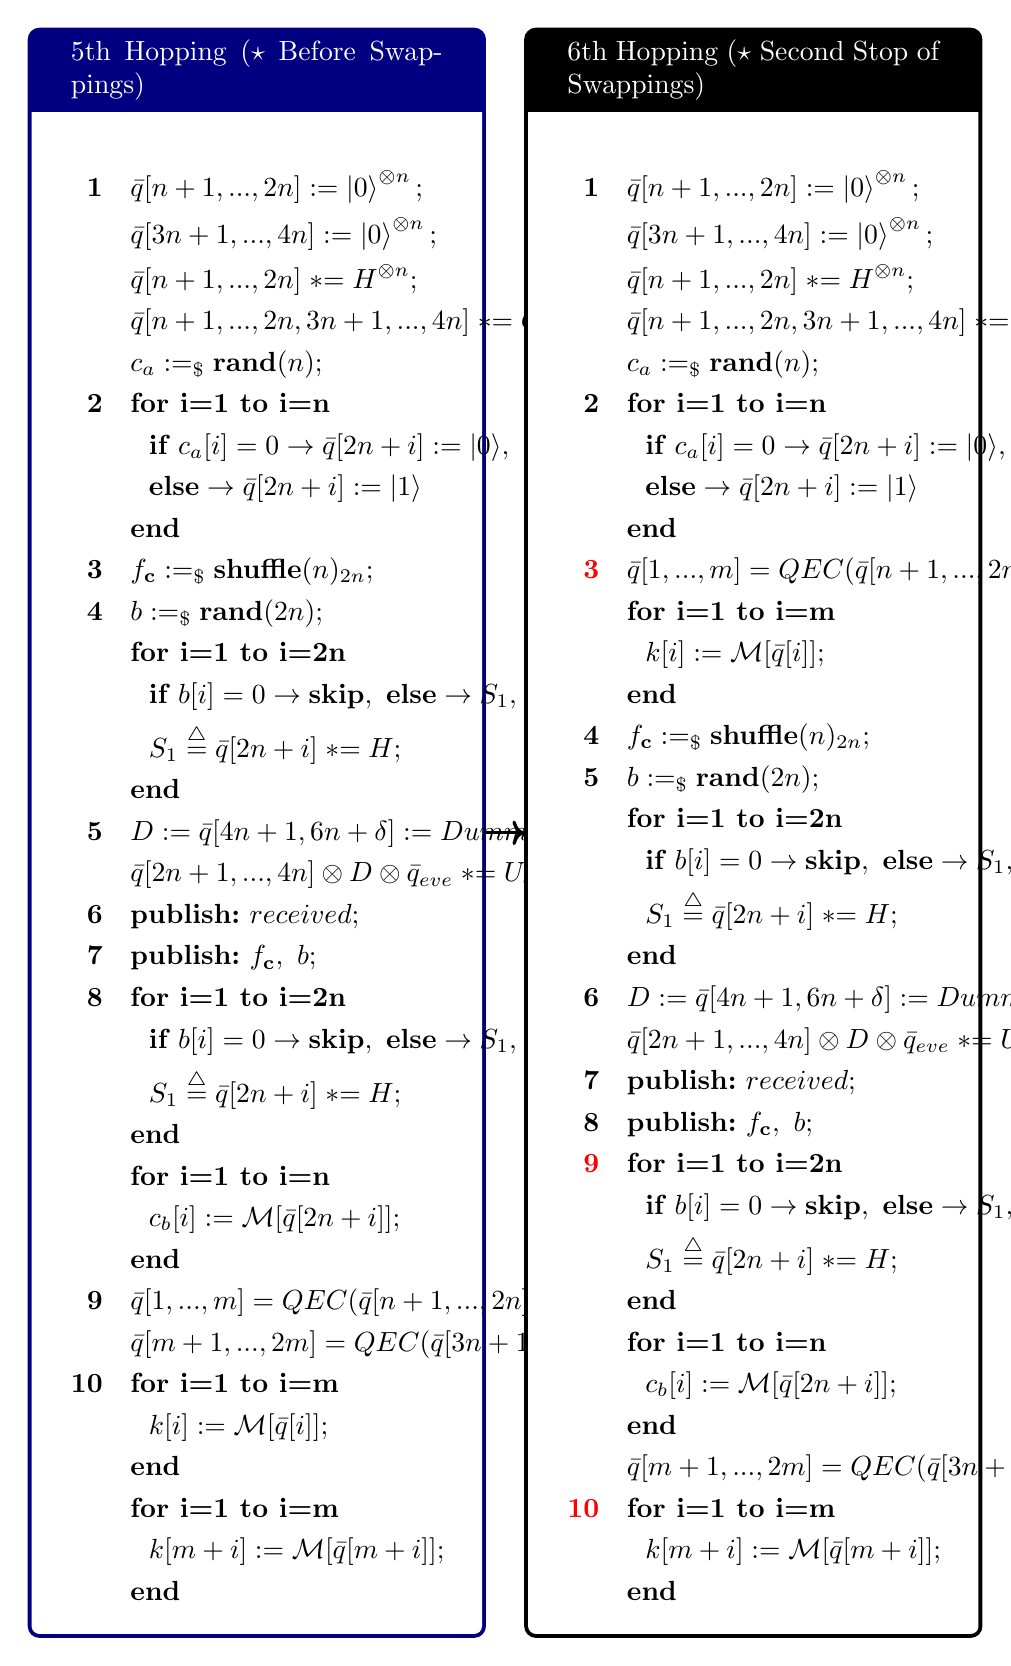
\begin{tikzpicture}[remember picture]

% Left box
\node[anchor=north west,inner sep=0pt,outer sep=0pt] (leftbox) at (0,0) {
\begin{minipage}[t]{0.48\textwidth}
\begin{tcolorbox}[colframe=blue!50!black, colback=white, title=5th Hopping ($\star$ Before Swappings), width=\textwidth]
\begin{align*}
    \textbf{{1}} \quad &\bar{q}[n+1,...,2n] := \ket{0}^{\otimes n};\\
    &\bar{q}[3n+1,...,4n] := \ket{0}^{\otimes n};\\
    \quad &\bar{q}[n+1,...,2n] \asteq H^{\otimes n}; \\
    &\bar{q}[n+1,...,2n,3n+1,...,4n] \asteq CNOT; \\
    & c_a :=_\$ \textbf{rand}(n); \\ 
    \textbf{{2}} \quad &\textbf{for~i=1~to~i=n}\\
    &~~ \textbf{if }  c_a[i] = 0 \rightarrow \bar{q}[2n+i] := |0\rangle,\\ &~~\textbf{else}   \rightarrow \bar{q}[2n+i] := |1\rangle\\
    &\textbf{end}\ \\
    \textbf{{3}} \quad & f_{\textbf{c}}:=_\$\textbf{shuffle}(n)_{2n}; \\
    \textbf{{4}} \quad & b :=_\$ \textbf{rand}(2n); \\
    &\textbf{for~i=1~to~i=2n}\\
    &~~ \textbf{if }  b[i] = 0 \rightarrow \textbf{skip},~\textbf{else}\rightarrow S_{1} ,\\
    &~~ S_{1}\stackrel{\triangle}{=}\bar{q}[2n+i] \asteq H ;\\
    &\textbf{end}\\
    \textbf{{5}} \quad & {D}:= \bar{q}[4n+1,6n+\delta]:=Dummy;\\     &\bar{q}[2n+1,...,4n]\otimes {D} \otimes \bar{q}_{eve} \asteq U_{\textbf{c}}(f_{\textbf{c}}); \\
    \textbf{{6}} \quad & \textbf{publish:}~ received;\\
    \textbf{{7}} \quad & \textbf{publish:}~ f_{\textbf{c}},~b;\\
    \textbf{{8}} \quad & \textbf{for~i=1~to~i=2n}\\
    &~~ \textbf{if }  b[i] = 0 \rightarrow \textbf{skip},~\textbf{else}\rightarrow S_{1} ,\\
    &~~ S_{1}\stackrel{\triangle}{=}\bar{q}[2n+i] \asteq H ;\\
    &\textbf{end}\\
    \quad & \textbf{for~i=1~to~i=n}\\
    &~~ c_b[i]:= \mathcal{M} [\bar{q}[2n+i]];\\
    &\textbf{end}\\
    \textbf{9} \quad & \bar{q}[1,...,m]=QEC(\bar{q}[n+1,...,2n])\\
    \quad & \bar{q}[m+1,...,2m]=QEC(\bar{q}[3n+1,...,4n])\\
    \textbf{10} \quad & \textbf{for~i=1~to~i=m}\\
    &~~ k[i]:= \mathcal{M} [\bar{q}[i]];\\
    &\textbf{end}
    \\
    & \textbf{for~i=1~to~i=m}\\
    &~~ k[m+i]:= \mathcal{M} [\bar{q}[m+i]];\\
    &\textbf{end}
\end{align*}
\end{tcolorbox}
\end{minipage}
};

% Right box
\node[anchor=north west,inner sep=0pt,outer sep=0pt] (rightbox) at (0.52\textwidth,0) {
\begin{minipage}[t]{0.48\textwidth}
\begin{tcolorbox}[colframe=black!50!black, colback=white, title=6th Hopping ($\star$ Second Stop of Swappings), width=\textwidth]
\begin{align*}
    \textbf{{1}} \quad &\bar{q}[n+1,...,2n] := \ket{0}^{\otimes n};\\
    &\bar{q}[3n+1,...,4n] := \ket{0}^{\otimes n};\\
    \quad &\bar{q}[n+1,...,2n] \asteq H^{\otimes n}; \\
    &\bar{q}[n+1,...,2n,3n+1,...,4n] \asteq CNOT; \\
    & c_a :=_\$ \textbf{rand}(n); \\ 
    \textbf{{2}} \quad &\textbf{for~i=1~to~i=n}\\
    &~~ \textbf{if }  c_a[i] = 0 \rightarrow \bar{q}[2n+i] := |0\rangle,\\ &~~\textbf{else}   \rightarrow \bar{q}[2n+i] := |1\rangle\\
    &\textbf{end}\ \\
    \textbf{\textcolor{red}{3}} \quad & \bar{q}[1,...,m]=QEC(\bar{q}[n+1,...,2n])\\
    \quad & \textbf{for~i=1~to~i=m}\\
    &~~ k[i]:= \mathcal{M} [\bar{q}[i]];\\
    &\textbf{end}\\
    \textbf{{4}} \quad & f_{\textbf{c}}:=_\$\textbf{shuffle}(n)_{2n}; \\
    \textbf{{5}} \quad & b :=_\$ \textbf{rand}(2n); \\
    &\textbf{for~i=1~to~i=2n}\\
    &~~ \textbf{if }  b[i] = 0 \rightarrow \textbf{skip},~\textbf{else}\rightarrow S_{1} ,\\
    &~~ S_{1}\stackrel{\triangle}{=}\bar{q}[2n+i] \asteq H ;\\
    &\textbf{end}\\
    \textbf{{6}} \quad & {D}:= \bar{q}[4n+1,6n+\delta]:=Dummy;\\     &\bar{q}[2n+1,...,4n]\otimes {D} \otimes \bar{q}_{eve} \asteq U_{\textbf{c}}(f_{\textbf{c}}); \\
    \textbf{{7}} \quad & \textbf{publish:}~ received;\\
    \textbf{{8}} \quad & \textbf{publish:}~ f_{\textbf{c}},~b;\\
    \textbf{\textcolor{red}{9}} \quad & \textbf{for~i=1~to~i=2n}\\
    &~~ \textbf{if }  b[i] = 0 \rightarrow \textbf{skip},~\textbf{else}\rightarrow S_{1} ,\\
    &~~ S_{1}\stackrel{\triangle}{=}\bar{q}[2n+i] \asteq H ;\\
    &\textbf{end}\\
    \quad & \textbf{for~i=1~to~i=n}\\
    &~~ c_b[i]:= \mathcal{M} [\bar{q}[2n+i]];\\
    &\textbf{end}\\
    \quad & \bar{q}[m+1,...,2m]=QEC(\bar{q}[3n+1,...,4n])\\
    \textbf{\textcolor{red}{10}} \quad 
    & \textbf{for~i=1~to~i=m}\\
    &~~ k[m+i]:= \mathcal{M} [\bar{q}[m+i]];\\
    &\textbf{end}
\end{align*}
\end{tcolorbox}
\end{minipage}
};

% Draw arrow between boxes
\draw[->, very thick] (leftbox.east) -- node[above]{} (rightbox.west);

\end{tikzpicture}
\newpage

\noindent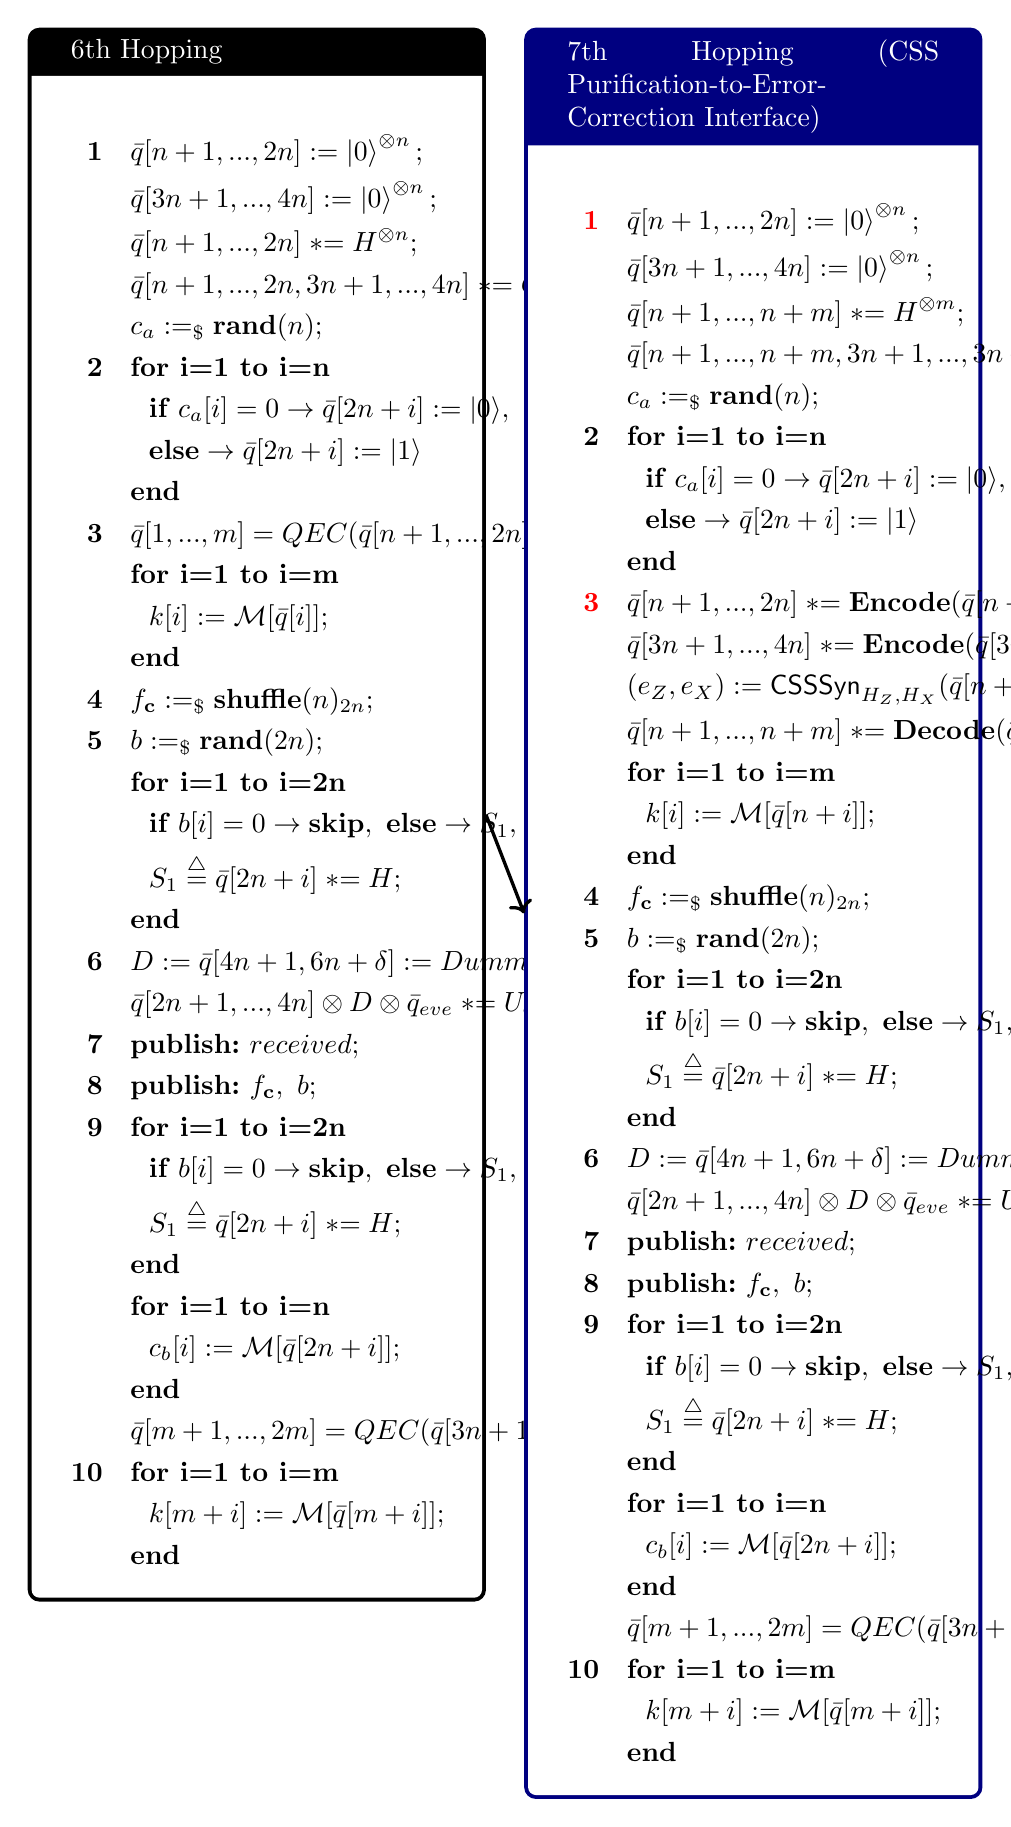
\begin{tikzpicture}[remember picture]

% Left box
\node[anchor=north west,inner sep=0pt,outer sep=0pt] (leftbox) at (0,0) {
\begin{minipage}[t]{0.48\textwidth}
\begin{tcolorbox}[colframe=black!75!black, colback=white, title=6th Hopping, width=\textwidth]
\begin{align*}
    \textbf{{1}} \quad &\bar{q}[n+1,...,2n] := \ket{0}^{\otimes n};\\
    &\bar{q}[3n+1,...,4n] := \ket{0}^{\otimes n};\\
    \quad &\bar{q}[n+1,...,2n] \asteq H^{\otimes n}; \\
    &\bar{q}[n+1,...,2n,3n+1,...,4n] \asteq CNOT; \\
    & c_a :=_\$ \textbf{rand}(n); \\ 
    \textbf{{2}} \quad &\textbf{for~i=1~to~i=n}\\
    &~~ \textbf{if }  c_a[i] = 0 \rightarrow \bar{q}[2n+i] := |0\rangle,\\ &~~\textbf{else}   \rightarrow \bar{q}[2n+i] := |1\rangle\\
    &\textbf{end}\ \\
    \textbf{{3}} \quad & \bar{q}[1,...,m]=QEC(\bar{q}[n+1,...,2n])\\
    \quad & \textbf{for~i=1~to~i=m}\\
    &~~ k[i]:= \mathcal{M} [\bar{q}[i]];\\
    &\textbf{end}\\
    \textbf{{4}} \quad & f_{\textbf{c}}:=_\$\textbf{shuffle}(n)_{2n}; \\
    \textbf{{5}} \quad & b :=_\$ \textbf{rand}(2n); \\
    &\textbf{for~i=1~to~i=2n}\\
    &~~ \textbf{if }  b[i] = 0 \rightarrow \textbf{skip},~\textbf{else}\rightarrow S_{1} ,\\
    &~~ S_{1}\stackrel{\triangle}{=}\bar{q}[2n+i] \asteq H ;\\
    &\textbf{end}\\
    \textbf{{6}} \quad & {D}:= \bar{q}[4n+1,6n+\delta]:=Dummy;\\     &\bar{q}[2n+1,...,4n]\otimes {D} \otimes \bar{q}_{eve} \asteq U_{\textbf{c}}(f_{\textbf{c}}); \\
    \textbf{{7}} \quad & \textbf{publish:}~ received;\\
    \textbf{{8}} \quad & \textbf{publish:}~ f_{\textbf{c}},~b;\\
    \textbf{{9}} \quad & \textbf{for~i=1~to~i=2n}\\
    &~~ \textbf{if }  b[i] = 0 \rightarrow \textbf{skip},~\textbf{else}\rightarrow S_{1} ,\\
    &~~ S_{1}\stackrel{\triangle}{=}\bar{q}[2n+i] \asteq H ;\\
    &\textbf{end}\\
    \quad & \textbf{for~i=1~to~i=n}\\
    &~~ c_b[i]:= \mathcal{M} [\bar{q}[2n+i]];\\
    &\textbf{end}\\
    \quad & \bar{q}[m+1,...,2m]=QEC(\bar{q}[3n+1,...,4n])\\
    \textbf{{10}} \quad 
    & \textbf{for~i=1~to~i=m}\\
    &~~ k[m+i]:= \mathcal{M} [\bar{q}[m+i]];\\
    &\textbf{end}
\end{align*}
\end{tcolorbox}
\end{minipage}
};

% Right box
\node[anchor=north west,inner sep=0pt,outer sep=0pt] (rightbox) at (0.52\textwidth,0) {
\begin{minipage}[t]{0.48\textwidth}
\begin{tcolorbox}[colframe=blue!50!black, colback=white, title=7th Hopping (CSS Purification-to-Error-Correction Interface), width=\textwidth]
\begin{align*}
    \textbf{\textcolor{red}{1}} \quad &\bar{q}[n+1,...,2n] := \ket{0}^{\otimes n};\\
    &\bar{q}[3n+1,...,4n] := \ket{0}^{\otimes n};\\
    \quad &\bar{q}[n+1,...,n+m] \asteq H^{\otimes m}; \\
    &\bar{q}[n+1,...,n+m,3n+1,...,3n+m] \asteq CNOT; \\
    & c_a :=_\$ \textbf{rand}(n); \\ 
    \textbf{{2}} \quad &\textbf{for~i=1~to~i=n}\\
    &~~ \textbf{if }  c_a[i] = 0 \rightarrow \bar{q}[2n+i] := |0\rangle,\\ &~~\textbf{else}   \rightarrow \bar{q}[2n+i] := |1\rangle\\
    &\textbf{end}\ \\
    \textbf{\textcolor{red}{3}} \quad &\bar{q}[n+1,...,2n]\asteq\textbf{Encode}(\bar{q}[n+1,...,n+m])\\
    &\bar{q}[3n+1,...,4n]\asteq\textbf{Encode}(\bar{q}[3n+1,...,3n+m])\\
    & (e_Z,e_X)  :=  \mathsf{CSSSyn}_{H_Z,H_X}  (\bar q[n+1,\ldots,2n];a_Z,a_X);\\
    & \bar{q}[n+1,...,n+m]\asteq\textbf{Decode}(\bar{q}[n+1,...,2n])\\
    \quad & \textbf{for~i=1~to~i=m}\\
    &~~ k[i]:= \mathcal{M} [\bar{q}[n+i]];\\
    &\textbf{end}\\
    \textbf{{4}} \quad & f_{\textbf{c}}:=_\$\textbf{shuffle}(n)_{2n}; \\
    \textbf{{5}} \quad & b :=_\$ \textbf{rand}(2n); \\
    &\textbf{for~i=1~to~i=2n}\\
    &~~ \textbf{if }  b[i] = 0 \rightarrow \textbf{skip},~\textbf{else}\rightarrow S_{1} ,\\
    &~~ S_{1}\stackrel{\triangle}{=}\bar{q}[2n+i] \asteq H ;\\
    &\textbf{end}\\
    \textbf{{6}} \quad & {D}:= \bar{q}[4n+1,6n+\delta]:=Dummy;\\     &\bar{q}[2n+1,...,4n]\otimes {D} \otimes \bar{q}_{eve} \asteq U_{\textbf{c}}(f_{\textbf{c}}); \\
    \textbf{{7}} \quad & \textbf{publish:}~ received;\\
    \textbf{{8}} \quad & \textbf{publish:}~ f_{\textbf{c}},~b;\\
    \textbf{{9}} \quad & \textbf{for~i=1~to~i=2n}\\
    &~~ \textbf{if }  b[i] = 0 \rightarrow \textbf{skip},~\textbf{else}\rightarrow S_{1} ,\\
    &~~ S_{1}\stackrel{\triangle}{=}\bar{q}[2n+i] \asteq H ;\\
    &\textbf{end}\\
    \quad & \textbf{for~i=1~to~i=n}\\
    &~~ c_b[i]:= \mathcal{M} [\bar{q}[2n+i]];\\
    &\textbf{end}\\
    \quad & \bar{q}[m+1,...,2m]=QEC(\bar{q}[3n+1,...,4n])\\
    \textbf{{10}} \quad 
    & \textbf{for~i=1~to~i=m}\\
    &~~ k[m+i]:= \mathcal{M} [\bar{q}[m+i]];\\
    &\textbf{end}
\end{align*}
\end{tcolorbox}
\end{minipage}
};

% Draw arrow between boxes
\draw[->, very thick] (leftbox.east) -- node[above]{} (rightbox.west);

\end{tikzpicture}
\newpage

\noindent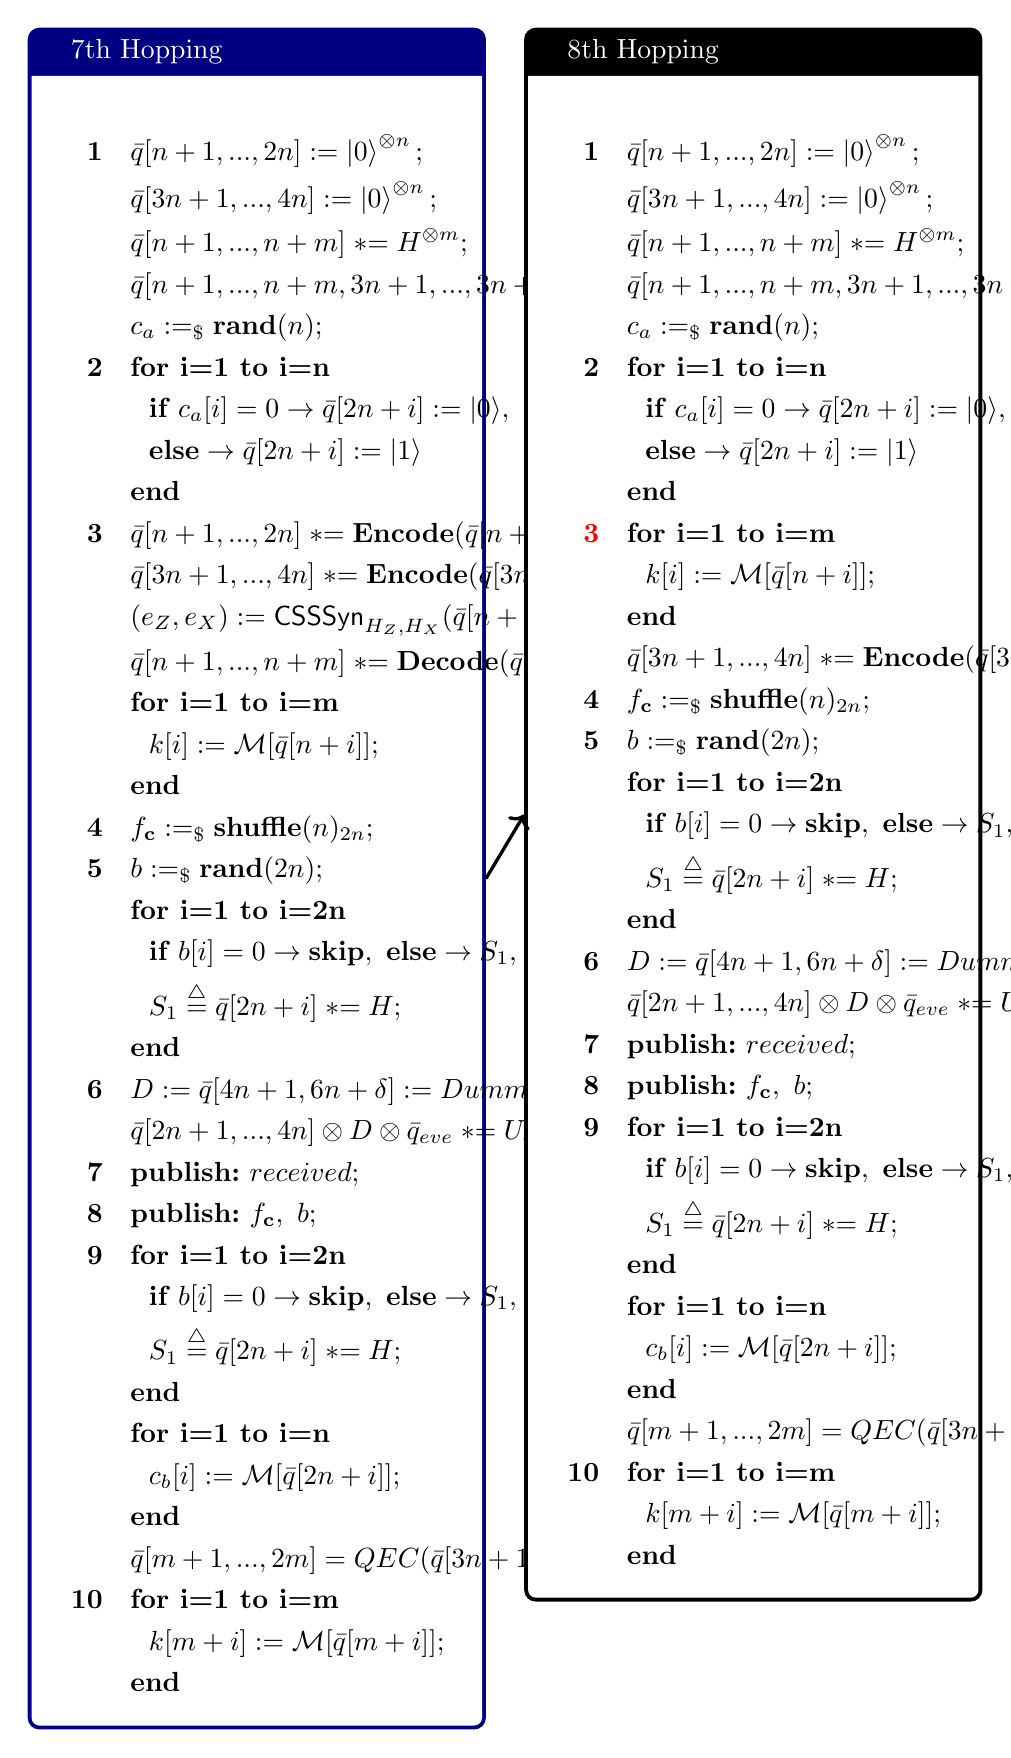
\begin{tikzpicture}[remember picture]

% Left box
\node[anchor=north west,inner sep=0pt,outer sep=0pt] (leftbox) at (0,0) {
\begin{minipage}[t]{0.48\textwidth}
\begin{tcolorbox}[colframe=blue!50!black, colback=white, title=7th Hopping, width=\textwidth]
\begin{align*}
    \textbf{{1}} \quad &\bar{q}[n+1,...,2n] := \ket{0}^{\otimes n};\\
    &\bar{q}[3n+1,...,4n] := \ket{0}^{\otimes n};\\
    \quad &\bar{q}[n+1,...,n+m] \asteq H^{\otimes m}; \\
    &\bar{q}[n+1,...,n+m,3n+1,...,3n+m] \asteq CNOT; \\
    & c_a :=_\$ \textbf{rand}(n); \\ 
    \textbf{{2}} \quad &\textbf{for~i=1~to~i=n}\\
    &~~ \textbf{if }  c_a[i] = 0 \rightarrow \bar{q}[2n+i] := |0\rangle,\\ &~~\textbf{else}   \rightarrow \bar{q}[2n+i] := |1\rangle\\
    &\textbf{end}\ \\
    \textbf{{3}} \quad &\bar{q}[n+1,...,2n]\asteq\textbf{Encode}(\bar{q}[n+1,...,n+m])\\
    &\bar{q}[3n+1,...,4n]\asteq\textbf{Encode}(\bar{q}[3n+1,...,3n+m])\\
    & (e_Z,e_X)  :=  \mathsf{CSSSyn}_{H_Z,H_X}  (\bar q[n+1,\ldots,2n];a_Z,a_X);\\
    & \bar{q}[n+1,...,n+m]\asteq\textbf{Decode}(\bar{q}[n+1,...,2n])\\
    \quad & \textbf{for~i=1~to~i=m}\\
    &~~ k[i]:= \mathcal{M} [\bar{q}[n+i]];\\
    &\textbf{end}\\
    \textbf{{4}} \quad & f_{\textbf{c}}:=_\$\textbf{shuffle}(n)_{2n}; \\
    \textbf{{5}} \quad & b :=_\$ \textbf{rand}(2n); \\
    &\textbf{for~i=1~to~i=2n}\\
    &~~ \textbf{if }  b[i] = 0 \rightarrow \textbf{skip},~\textbf{else}\rightarrow S_{1} ,\\
    &~~ S_{1}\stackrel{\triangle}{=}\bar{q}[2n+i] \asteq H ;\\
    &\textbf{end}\\
    \textbf{{6}} \quad & {D}:= \bar{q}[4n+1,6n+\delta]:=Dummy;\\     &\bar{q}[2n+1,...,4n]\otimes {D} \otimes \bar{q}_{eve} \asteq U_{\textbf{c}}(f_{\textbf{c}}); \\
    \textbf{{7}} \quad & \textbf{publish:}~ received;\\
    \textbf{{8}} \quad & \textbf{publish:}~ f_{\textbf{c}},~b;\\
    \textbf{{9}} \quad & \textbf{for~i=1~to~i=2n}\\
    &~~ \textbf{if }  b[i] = 0 \rightarrow \textbf{skip},~\textbf{else}\rightarrow S_{1} ,\\
    &~~ S_{1}\stackrel{\triangle}{=}\bar{q}[2n+i] \asteq H ;\\
    &\textbf{end}\\
    \quad & \textbf{for~i=1~to~i=n}\\
    &~~ c_b[i]:= \mathcal{M} [\bar{q}[2n+i]];\\
    &\textbf{end}\\
    \quad & \bar{q}[m+1,...,2m]=QEC(\bar{q}[3n+1,...,4n])\\
    \textbf{{10}} \quad 
    & \textbf{for~i=1~to~i=m}\\
    &~~ k[m+i]:= \mathcal{M} [\bar{q}[m+i]];\\
    &\textbf{end}
\end{align*}
\end{tcolorbox}
\end{minipage}
};
% Right box
\node[anchor=north west,inner sep=0pt,outer sep=0pt] (rightbox) at (0.52\textwidth,0) {
\begin{minipage}[t]{0.48\textwidth}
\begin{tcolorbox}[colframe=black!50!black, colback=white, title=8th Hopping, width=\textwidth]
\begin{align*}
    \textbf{{1}} \quad &\bar{q}[n+1,...,2n] := \ket{0}^{\otimes n};\\
    &\bar{q}[3n+1,...,4n] := \ket{0}^{\otimes n};\\
    \quad &\bar{q}[n+1,...,n+m] \asteq H^{\otimes m}; \\
    &\bar{q}[n+1,...,n+m,3n+1,...,3n+m] \asteq CNOT; \\
    & c_a :=_\$ \textbf{rand}(n); \\ 
    \textbf{{2}} \quad &\textbf{for~i=1~to~i=n}\\
    &~~ \textbf{if }  c_a[i] = 0 \rightarrow \bar{q}[2n+i] := |0\rangle,\\ &~~\textbf{else}   \rightarrow \bar{q}[2n+i] := |1\rangle\\
    &\textbf{end}\ \\
    \textbf{\textcolor{red}{3}} \quad 
    & \textbf{for~i=1~to~i=m}\\
    &~~ k[i]:= \mathcal{M} [\bar{q}[n+i]];\\
    &\textbf{end}\\
    &\bar{q}[3n+1,...,4n]\asteq\textbf{Encode}(\bar{q}[3n+1,...,3n+m])\\
    \textbf{{4}} \quad & f_{\textbf{c}}:=_\$\textbf{shuffle}(n)_{2n}; \\
    \textbf{{5}} \quad & b :=_\$ \textbf{rand}(2n); \\
    &\textbf{for~i=1~to~i=2n}\\
    &~~ \textbf{if }  b[i] = 0 \rightarrow \textbf{skip},~\textbf{else}\rightarrow S_{1} ,\\
    &~~ S_{1}\stackrel{\triangle}{=}\bar{q}[2n+i] \asteq H ;\\
    &\textbf{end}\\
    \textbf{{6}} \quad & {D}:= \bar{q}[4n+1,6n+\delta]:=Dummy;\\     &\bar{q}[2n+1,...,4n]\otimes {D} \otimes \bar{q}_{eve} \asteq U_{\textbf{c}}(f_{\textbf{c}}); \\
    \textbf{{7}} \quad & \textbf{publish:}~ received;\\
    \textbf{{8}} \quad & \textbf{publish:}~ f_{\textbf{c}},~b;\\
    \textbf{{9}} \quad & \textbf{for~i=1~to~i=2n}\\
    &~~ \textbf{if }  b[i] = 0 \rightarrow \textbf{skip},~\textbf{else}\rightarrow S_{1} ,\\
    &~~ S_{1}\stackrel{\triangle}{=}\bar{q}[2n+i] \asteq H ;\\
    &\textbf{end}\\
    \quad & \textbf{for~i=1~to~i=n}\\
    &~~ c_b[i]:= \mathcal{M} [\bar{q}[2n+i]];\\
    &\textbf{end}\\
    \quad & \bar{q}[m+1,...,2m]=QEC(\bar{q}[3n+1,...,4n])\\
    \textbf{{10}} \quad 
    & \textbf{for~i=1~to~i=m}\\
    &~~ k[m+i]:= \mathcal{M} [\bar{q}[m+i]];\\
    &\textbf{end}
\end{align*}
\end{tcolorbox}
\end{minipage}
};


% Draw arrow between boxes
\draw[->, very thick] (leftbox.east) -- node[above]{} (rightbox.west);

\end{tikzpicture}


\newpage

\noindent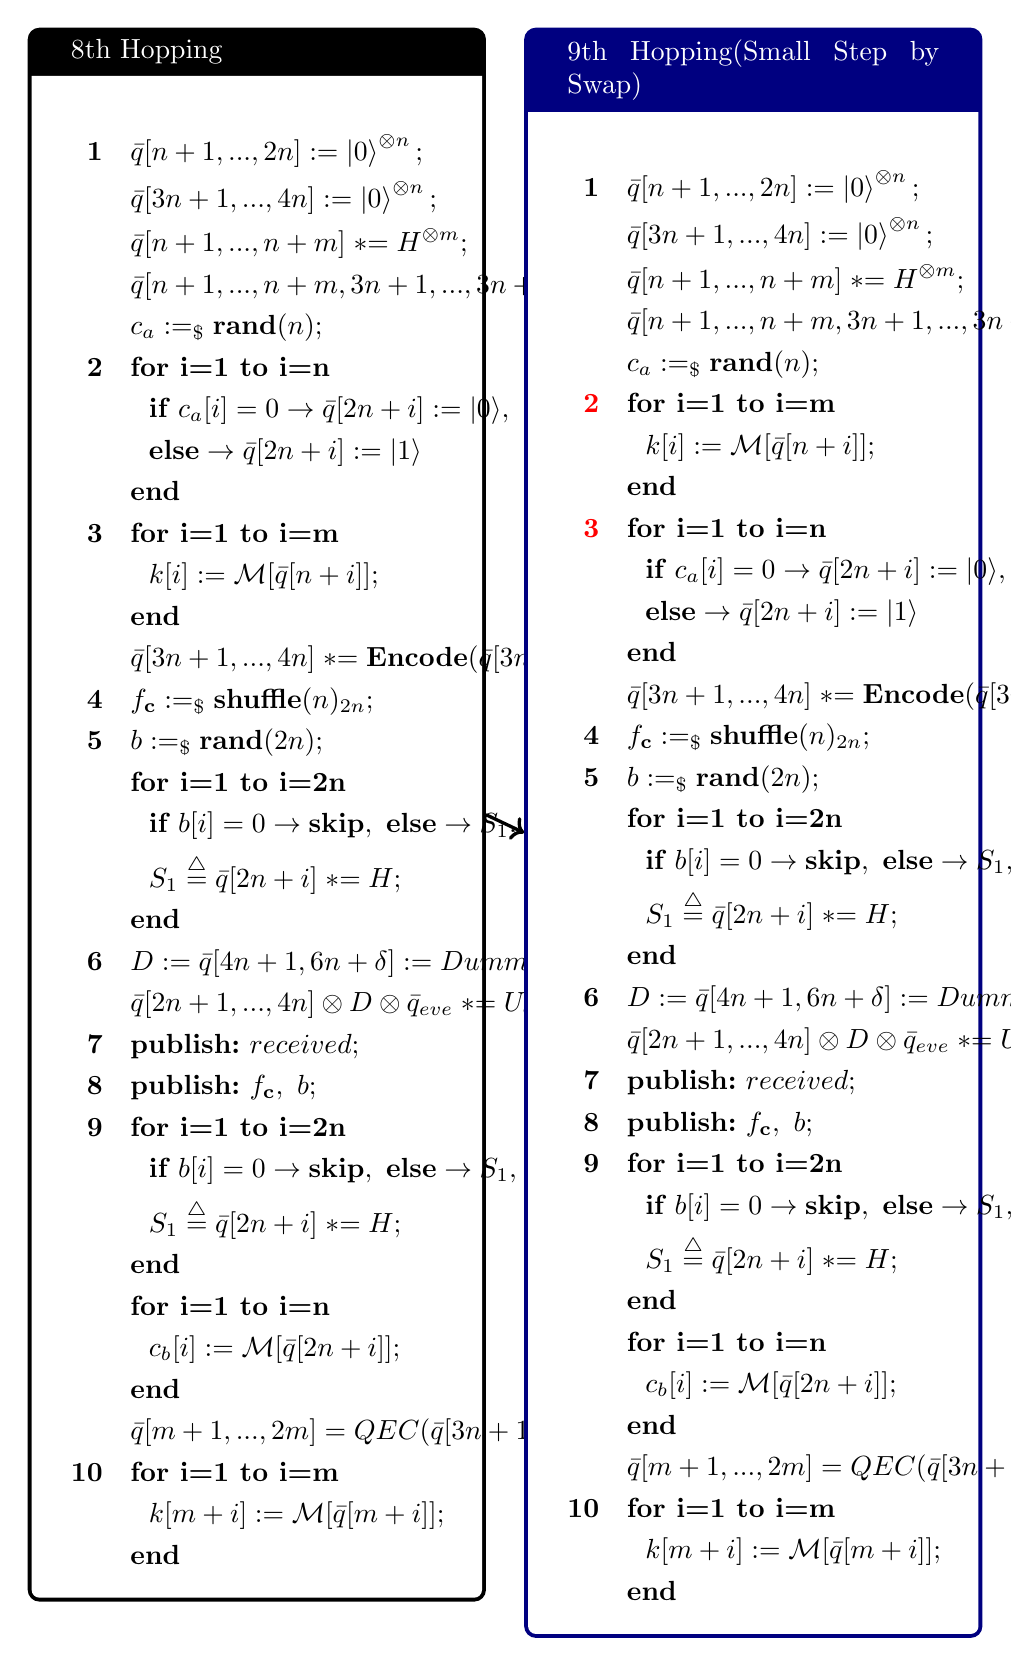
\begin{tikzpicture}[remember picture]

% Left box
\node[anchor=north west,inner sep=0pt,outer sep=0pt] (leftbox) at (0,0) {
\begin{minipage}[t]{0.48\textwidth}
\begin{tcolorbox}[colframe=black!75!black, colback=white, title=8th Hopping, width=\textwidth]
\begin{align*}
    \textbf{{1}} \quad &\bar{q}[n+1,...,2n] := \ket{0}^{\otimes n};\\
    &\bar{q}[3n+1,...,4n] := \ket{0}^{\otimes n};\\
    \quad &\bar{q}[n+1,...,n+m] \asteq H^{\otimes m}; \\
    &\bar{q}[n+1,...,n+m,3n+1,...,3n+m] \asteq CNOT; \\
    & c_a :=_\$ \textbf{rand}(n); \\ 
    \textbf{{2}} \quad &\textbf{for~i=1~to~i=n}\\
    &~~ \textbf{if }  c_a[i] = 0 \rightarrow \bar{q}[2n+i] := |0\rangle,\\ &~~\textbf{else}   \rightarrow \bar{q}[2n+i] := |1\rangle\\
    &\textbf{end}\ \\
    \textbf{{3}} \quad 
    & \textbf{for~i=1~to~i=m}\\
    &~~ k[i]:= \mathcal{M} [\bar{q}[n+i]];\\
    &\textbf{end}\\
    &\bar{q}[3n+1,...,4n]\asteq\textbf{Encode}(\bar{q}[3n+1,...,3n+m])\\
    \textbf{{4}} \quad & f_{\textbf{c}}:=_\$\textbf{shuffle}(n)_{2n}; \\
    \textbf{{5}} \quad & b :=_\$ \textbf{rand}(2n); \\
    &\textbf{for~i=1~to~i=2n}\\
    &~~ \textbf{if }  b[i] = 0 \rightarrow \textbf{skip},~\textbf{else}\rightarrow S_{1} ,\\
    &~~ S_{1}\stackrel{\triangle}{=}\bar{q}[2n+i] \asteq H ;\\
    &\textbf{end}\\
    \textbf{{6}} \quad & {D}:= \bar{q}[4n+1,6n+\delta]:=Dummy;\\     &\bar{q}[2n+1,...,4n]\otimes {D} \otimes \bar{q}_{eve} \asteq U_{\textbf{c}}(f_{\textbf{c}}); \\
    \textbf{{7}} \quad & \textbf{publish:}~ received;\\
    \textbf{{8}} \quad & \textbf{publish:}~ f_{\textbf{c}},~b;\\
    \textbf{{9}} \quad & \textbf{for~i=1~to~i=2n}\\
    &~~ \textbf{if }  b[i] = 0 \rightarrow \textbf{skip},~\textbf{else}\rightarrow S_{1} ,\\
    &~~ S_{1}\stackrel{\triangle}{=}\bar{q}[2n+i] \asteq H ;\\
    &\textbf{end}\\
    \quad & \textbf{for~i=1~to~i=n}\\
    &~~ c_b[i]:= \mathcal{M} [\bar{q}[2n+i]];\\
    &\textbf{end}\\
    \quad & \bar{q}[m+1,...,2m]=QEC(\bar{q}[3n+1,...,4n])\\
    \textbf{{10}} \quad 
    & \textbf{for~i=1~to~i=m}\\
    &~~ k[m+i]:= \mathcal{M} [\bar{q}[m+i]];\\
    &\textbf{end}
\end{align*}
\end{tcolorbox}
\end{minipage}
};

% Right box
\node[anchor=north west,inner sep=0pt,outer sep=0pt] (rightbox) at (0.52\textwidth,0) {
\begin{minipage}[t]{0.48\textwidth}
\begin{tcolorbox}[colframe=blue!50!black, colback=white, title=9th Hopping(Small Step by Swap), width=\textwidth]
\begin{align*}
    \textbf{{1}} \quad &\bar{q}[n+1,...,2n] := \ket{0}^{\otimes n};\\
    &\bar{q}[3n+1,...,4n] := \ket{0}^{\otimes n};\\
    \quad &\bar{q}[n+1,...,n+m] \asteq H^{\otimes m}; \\
    &\bar{q}[n+1,...,n+m,3n+1,...,3n+m] \asteq CNOT; \\
    & c_a :=_\$ \textbf{rand}(n); \\ 
    \textbf{\textcolor{red}{2}} \quad 
    & \textbf{for~i=1~to~i=m}\\
    &~~ k[i]:= \mathcal{M} [\bar{q}[n+i]];\\
    &\textbf{end}\\
    \textbf{\textcolor{red}{3}} \quad 
    &\textbf{for~i=1~to~i=n}\\
    &~~ \textbf{if }  c_a[i] = 0 \rightarrow \bar{q}[2n+i] := |0\rangle,\\ &~~\textbf{else}   \rightarrow \bar{q}[2n+i] := |1\rangle\\
    &\textbf{end}\ \\
    &\bar{q}[3n+1,...,4n]\asteq\textbf{Encode}(\bar{q}[3n+1,...,3n+m])\\ 
    \textbf{{4}} \quad & f_{\textbf{c}}:=_\$\textbf{shuffle}(n)_{2n}; \\
    \textbf{{5}} \quad & b :=_\$ \textbf{rand}(2n); \\
    &\textbf{for~i=1~to~i=2n}\\
    &~~ \textbf{if }  b[i] = 0 \rightarrow \textbf{skip},~\textbf{else}\rightarrow S_{1} ,\\
    &~~ S_{1}\stackrel{\triangle}{=}\bar{q}[2n+i] \asteq H ;\\
    &\textbf{end}\\
    \textbf{{6}} \quad & {D}:= \bar{q}[4n+1,6n+\delta]:=Dummy;\\     &\bar{q}[2n+1,...,4n]\otimes {D} \otimes \bar{q}_{eve} \asteq U_{\textbf{c}}(f_{\textbf{c}}); \\
    \textbf{{7}} \quad & \textbf{publish:}~ received;\\
    \textbf{{8}} \quad & \textbf{publish:}~ f_{\textbf{c}},~b;\\
    \textbf{{9}} \quad & \textbf{for~i=1~to~i=2n}\\
    &~~ \textbf{if }  b[i] = 0 \rightarrow \textbf{skip},~\textbf{else}\rightarrow S_{1} ,\\
    &~~ S_{1}\stackrel{\triangle}{=}\bar{q}[2n+i] \asteq H ;\\
    &\textbf{end}\\
    \quad & \textbf{for~i=1~to~i=n}\\
    &~~ c_b[i]:= \mathcal{M} [\bar{q}[2n+i]];\\
    &\textbf{end}\\
    \quad & \bar{q}[m+1,...,2m]=QEC(\bar{q}[3n+1,...,4n])\\
    \textbf{{10}} \quad 
    & \textbf{for~i=1~to~i=m}\\
    &~~ k[m+i]:= \mathcal{M} [\bar{q}[m+i]];\\
    &\textbf{end}
\end{align*}
\end{tcolorbox}
\end{minipage}
};

% Draw arrow between boxes
\draw[->, very thick] (leftbox.east) -- node[above]{} (rightbox.west);

\end{tikzpicture}
\newpage

\noindent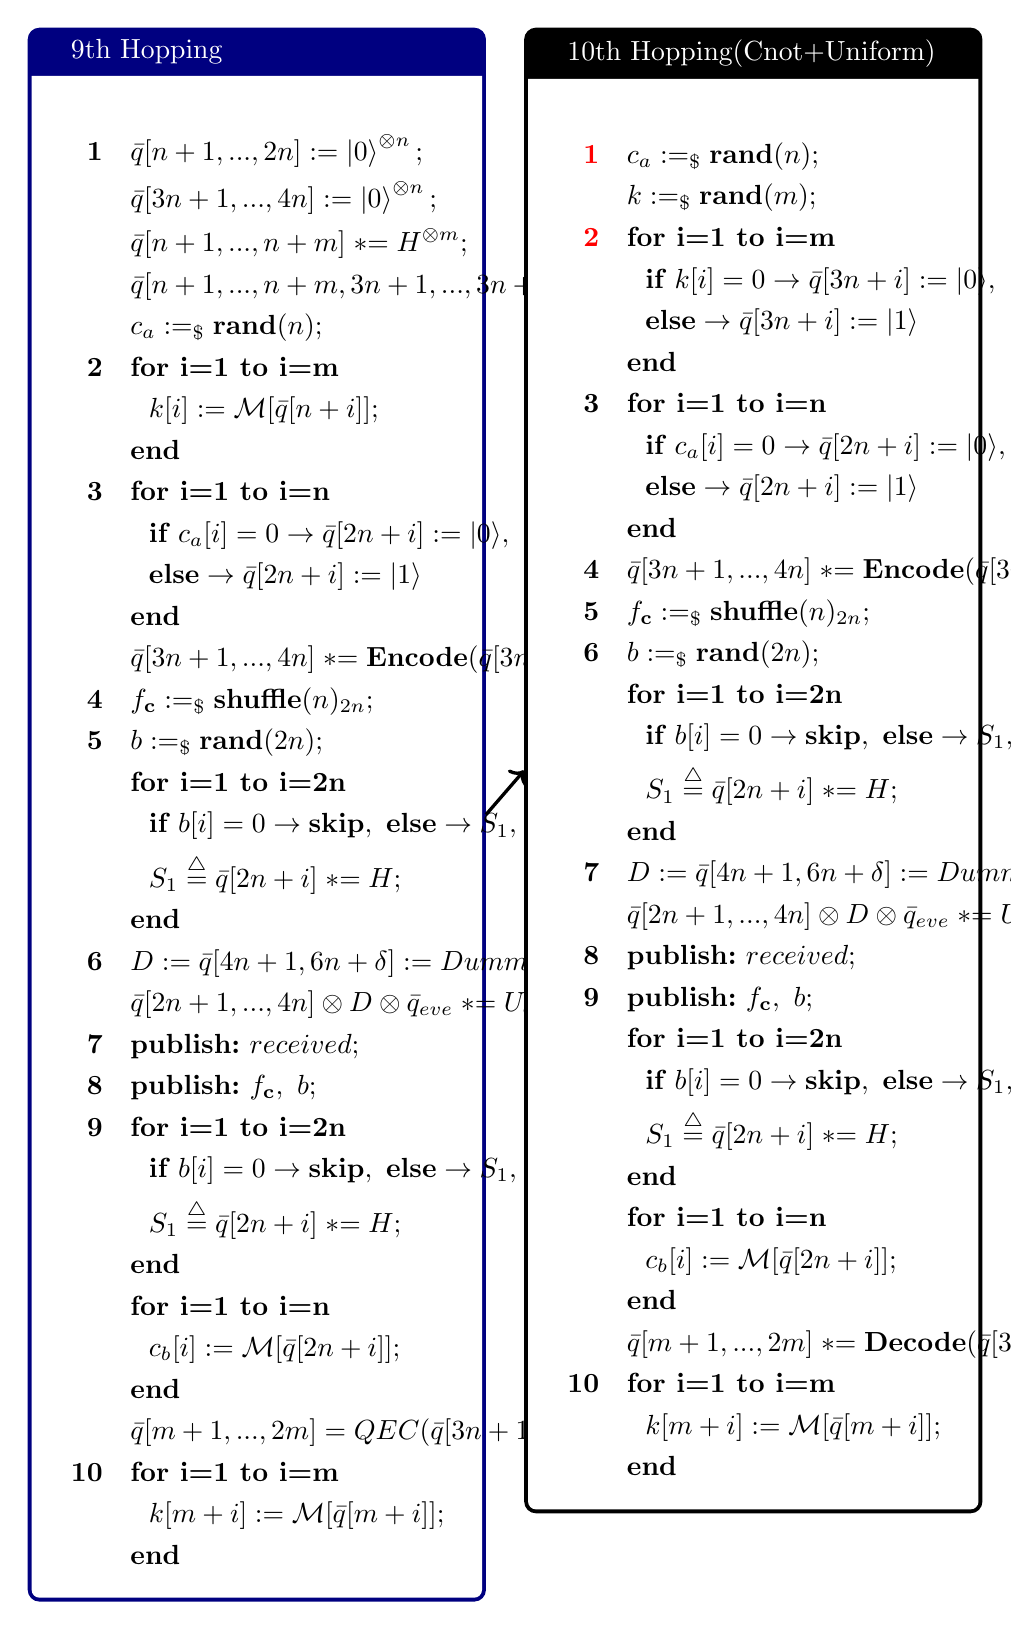
\begin{tikzpicture}[remember picture]

% Left box
\node[anchor=north west,inner sep=0pt,outer sep=0pt] (leftbox) at (0,0) {
\begin{minipage}[t]{0.48\textwidth}
\begin{tcolorbox}[colframe=blue!50!black, colback=white, title=9th Hopping, width=\textwidth]
\begin{align*}
    \textbf{{1}} \quad &\bar{q}[n+1,...,2n] := \ket{0}^{\otimes n};\\
    &\bar{q}[3n+1,...,4n] := \ket{0}^{\otimes n};\\
    \quad &\bar{q}[n+1,...,n+m] \asteq H^{\otimes m}; \\
    &\bar{q}[n+1,...,n+m,3n+1,...,3n+m] \asteq CNOT; \\
    & c_a :=_\$ \textbf{rand}(n); \\ 
    \textbf{{2}} \quad 
    & \textbf{for~i=1~to~i=m}\\
    &~~ k[i]:= \mathcal{M} [\bar{q}[n+i]];\\
    &\textbf{end}\\
    \textbf{{3}} \quad 
    &\textbf{for~i=1~to~i=n}\\
    &~~ \textbf{if }  c_a[i] = 0 \rightarrow \bar{q}[2n+i] := |0\rangle,\\ &~~\textbf{else}   \rightarrow \bar{q}[2n+i] := |1\rangle\\
    &\textbf{end}\ \\
    &\bar{q}[3n+1,...,4n]\asteq\textbf{Encode}(\bar{q}[3n+1,...,3n+m])\\ 
    \textbf{{4}} \quad & f_{\textbf{c}}:=_\$\textbf{shuffle}(n)_{2n}; \\
    \textbf{{5}} \quad & b :=_\$ \textbf{rand}(2n); \\
    &\textbf{for~i=1~to~i=2n}\\
    &~~ \textbf{if }  b[i] = 0 \rightarrow \textbf{skip},~\textbf{else}\rightarrow S_{1} ,\\
    &~~ S_{1}\stackrel{\triangle}{=}\bar{q}[2n+i] \asteq H ;\\
    &\textbf{end}\\
    \textbf{{6}} \quad & {D}:= \bar{q}[4n+1,6n+\delta]:=Dummy;\\     &\bar{q}[2n+1,...,4n]\otimes {D} \otimes \bar{q}_{eve} \asteq U_{\textbf{c}}(f_{\textbf{c}}); \\
    \textbf{{7}} \quad & \textbf{publish:}~ received;\\
    \textbf{{8}} \quad & \textbf{publish:}~ f_{\textbf{c}},~b;\\
    \textbf{{9}} \quad & \textbf{for~i=1~to~i=2n}\\
    &~~ \textbf{if }  b[i] = 0 \rightarrow \textbf{skip},~\textbf{else}\rightarrow S_{1} ,\\
    &~~ S_{1}\stackrel{\triangle}{=}\bar{q}[2n+i] \asteq H ;\\
    &\textbf{end}\\
    \quad & \textbf{for~i=1~to~i=n}\\
    &~~ c_b[i]:= \mathcal{M} [\bar{q}[2n+i]];\\
    &\textbf{end}\\
    \quad & \bar{q}[m+1,...,2m]=QEC(\bar{q}[3n+1,...,4n])\\
    \textbf{{10}} \quad 
    & \textbf{for~i=1~to~i=m}\\
    &~~ k[m+i]:= \mathcal{M} [\bar{q}[m+i]];\\
    &\textbf{end}
\end{align*}
\end{tcolorbox}
\end{minipage}
};

% Right box
\node[anchor=north west,inner sep=0pt,outer sep=0pt] (rightbox) at (0.52\textwidth,0) {
\begin{minipage}[t]{0.48\textwidth}
\begin{tcolorbox}[colframe=black!50!black, colback=white, title=10th Hopping(Cnot+Uniform), width=\textwidth]
\begin{align*}
    \textbf{\textcolor{red}{1}} \quad 
    & c_a :=_\$ \textbf{rand}(n); \\ 
    & k :=_\$ \textbf{rand}(m); \\  \textbf{\textcolor{red}{2}} \quad &\textbf{for~i=1~to~i=m}\\
    &~~ \textbf{if }  k[i] = 0 \rightarrow \bar{q}[3n+i] := |0\rangle,\\ &~~\textbf{else}   \rightarrow \bar{q}[3n+i] := |1\rangle\\
    &\textbf{end}\ \\
    \textbf{{3}} \quad 
    &\textbf{for~i=1~to~i=n}\\
    &~~ \textbf{if }  c_a[i] = 0 \rightarrow \bar{q}[2n+i] := |0\rangle,\\ &~~\textbf{else}   \rightarrow \bar{q}[2n+i] := |1\rangle\\
    &\textbf{end}\ \\
    \textbf{{4}} \quad 
    &\bar{q}[3n+1,...,4n]\asteq\textbf{Encode}(\bar{q}[3n+1,...,3n+m])\\
    \textbf{{5}} \quad & f_{\textbf{c}}:=_\$\textbf{shuffle}(n)_{2n}; \\
    \textbf{{6}} \quad & b :=_\$ \textbf{rand}(2n); \\
    &\textbf{for~i=1~to~i=2n}\\
    &~~ \textbf{if }  b[i] = 0 \rightarrow \textbf{skip},~\textbf{else}\rightarrow S_{1} ,\\
    &~~ S_{1}\stackrel{\triangle}{=}\bar{q}[2n+i] \asteq H ;\\
    &\textbf{end}\\
    \textbf{{7}} \quad & {D}:= \bar{q}[4n+1,6n+\delta]:=Dummy;\\     &\bar{q}[2n+1,...,4n]\otimes {D} \otimes \bar{q}_{eve} \asteq U_{\textbf{c}}(f_{\textbf{c}}); \\
    \textbf{{8}} \quad & \textbf{publish:}~ received;\\
    \textbf{{9}} \quad & \textbf{publish:}~ f_{\textbf{c}},~b;\\
    \quad & \textbf{for~i=1~to~i=2n}\\
    &~~ \textbf{if }  b[i] = 0 \rightarrow \textbf{skip},~\textbf{else}\rightarrow S_{1} ,\\
    &~~ S_{1}\stackrel{\triangle}{=}\bar{q}[2n+i] \asteq H ;\\
    &\textbf{end}\\
    \quad & \textbf{for~i=1~to~i=n}\\
    &~~ c_b[i]:= \mathcal{M} [\bar{q}[2n+i]];\\
    &\textbf{end}\\
    \quad & \bar{q}[m+1,...,2m]\asteq\textbf{Decode}(\bar{q}[3n+1,...,4n])\\
    \textbf{{10}} \quad 
    & \textbf{for~i=1~to~i=m}\\
    &~~ k[m+i]:= \mathcal{M} [\bar{q}[m+i]];\\
    &\textbf{end}
\end{align*}
\end{tcolorbox}
\end{minipage}
};

% Draw arrow between boxes
\draw[->, very thick] (leftbox.east) -- node[above]{} (rightbox.west);

\end{tikzpicture}
\newpage

\noindent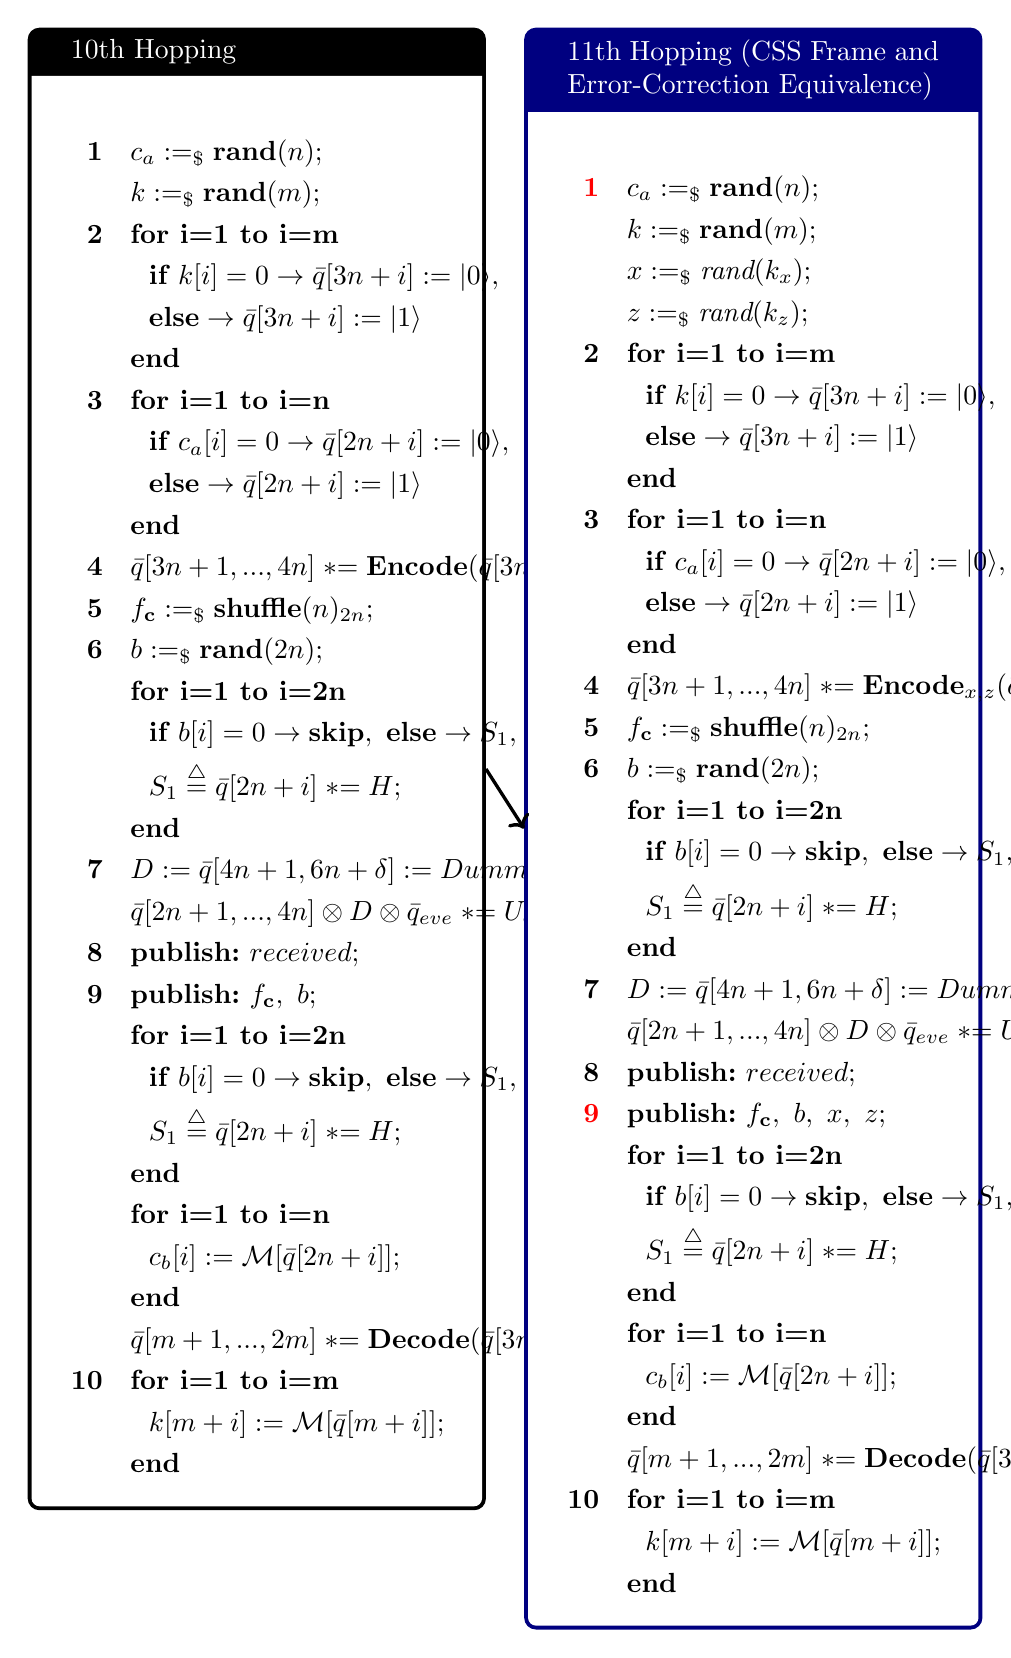
\begin{tikzpicture}[remember picture]

% Left box
\node[anchor=north west,inner sep=0pt,outer sep=0pt] (leftbox) at (0,0) {
\begin{minipage}[t]{0.48\textwidth}
\begin{tcolorbox}[colframe=black!50!black, colback=white, title=10th Hopping, width=\textwidth]
\begin{align*}
    \textbf{{1}} \quad 
    & c_a :=_\$ \textbf{rand}(n); \\ 
    & k :=_\$ \textbf{rand}(m); \\  \textbf{{2}} \quad &\textbf{for~i=1~to~i=m}\\
    &~~ \textbf{if }  k[i] = 0 \rightarrow \bar{q}[3n+i] := |0\rangle,\\ &~~\textbf{else}   \rightarrow \bar{q}[3n+i] := |1\rangle\\
    &\textbf{end}\ \\
    \textbf{{3}} \quad 
    &\textbf{for~i=1~to~i=n}\\
    &~~ \textbf{if }  c_a[i] = 0 \rightarrow \bar{q}[2n+i] := |0\rangle,\\ &~~\textbf{else}   \rightarrow \bar{q}[2n+i] := |1\rangle\\
    &\textbf{end}\ \\
    \textbf{{4}} \quad 
    &\bar{q}[3n+1,...,4n]\asteq\textbf{Encode}(\bar{q}[3n+1,...,3n+m])\\
    \textbf{{5}} \quad & f_{\textbf{c}}:=_\$\textbf{shuffle}(n)_{2n}; \\
    \textbf{{6}} \quad & b :=_\$ \textbf{rand}(2n); \\
    &\textbf{for~i=1~to~i=2n}\\
    &~~ \textbf{if }  b[i] = 0 \rightarrow \textbf{skip},~\textbf{else}\rightarrow S_{1} ,\\
    &~~ S_{1}\stackrel{\triangle}{=}\bar{q}[2n+i] \asteq H ;\\
    &\textbf{end}\\
    \textbf{{7}} \quad & {D}:= \bar{q}[4n+1,6n+\delta]:=Dummy;\\     &\bar{q}[2n+1,...,4n]\otimes {D} \otimes \bar{q}_{eve} \asteq U_{\textbf{c}}(f_{\textbf{c}}); \\
    \textbf{{8}} \quad & \textbf{publish:}~ received;\\
    \textbf{{9}} \quad & \textbf{publish:}~ f_{\textbf{c}},~b;\\
    \quad & \textbf{for~i=1~to~i=2n}\\
    &~~ \textbf{if }  b[i] = 0 \rightarrow \textbf{skip},~\textbf{else}\rightarrow S_{1} ,\\
    &~~ S_{1}\stackrel{\triangle}{=}\bar{q}[2n+i] \asteq H ;\\
    &\textbf{end}\\
    \quad & \textbf{for~i=1~to~i=n}\\
    &~~ c_b[i]:= \mathcal{M} [\bar{q}[2n+i]];\\
    &\textbf{end}\\
    \quad & \bar{q}[m+1,...,2m]\asteq\textbf{Decode}(\bar{q}[3n+1,...,4n])\\
    \textbf{{10}} \quad 
    & \textbf{for~i=1~to~i=m}\\
    &~~ k[m+i]:= \mathcal{M} [\bar{q}[m+i]];\\
    &\textbf{end}
\end{align*}
\end{tcolorbox}
\end{minipage}
};

% Right box
\node[anchor=north west,inner sep=0pt,outer sep=0pt] (rightbox) at (0.52\textwidth,0) {
\begin{minipage}[t]{0.48\textwidth}
\begin{tcolorbox}[colframe=blue!50!black, colback=white, title=11th Hopping (CSS Frame and Error-Correction Equivalence), width=\textwidth]
\begin{align*}
    \textbf{\textcolor{red}{1}} \quad 
    & c_a :=_\$ \textbf{rand}(n); \\ 
    & k :=_\$ \textbf{rand}(m); \\ 
    & x :=_\$ \textit{rand}(k_x); \\
    & z :=_\$ \textit{rand}(k_z); \\ \textbf{{2}} \quad &\textbf{for~i=1~to~i=m}\\
    &~~ \textbf{if }  k[i] = 0 \rightarrow \bar{q}[3n+i] := |0\rangle,\\ &~~\textbf{else}   \rightarrow \bar{q}[3n+i] := |1\rangle\\
    &\textbf{end}\ \\
    \textbf{{3}} \quad 
    &\textbf{for~i=1~to~i=n}\\
    &~~ \textbf{if }  c_a[i] = 0 \rightarrow \bar{q}[2n+i] := |0\rangle,\\ &~~\textbf{else}   \rightarrow \bar{q}[2n+i] := |1\rangle\\
    &\textbf{end}\ \\
    \textbf{{4}} \quad 
    &\bar{q}[3n+1,...,4n]\asteq\textbf{Encode}_{x,z}(\bar{q}[3n+1,...,3n+m])\\
    \textbf{{5}} \quad & f_{\textbf{c}}:=_\$\textbf{shuffle}(n)_{2n}; \\
    \textbf{{6}} \quad & b :=_\$ \textbf{rand}(2n); \\
    &\textbf{for~i=1~to~i=2n}\\
    &~~ \textbf{if }  b[i] = 0 \rightarrow \textbf{skip},~\textbf{else}\rightarrow S_{1} ,\\
    &~~ S_{1}\stackrel{\triangle}{=}\bar{q}[2n+i] \asteq H ;\\
    &\textbf{end}\\
    \textbf{{7}} \quad & {D}:= \bar{q}[4n+1,6n+\delta]:=Dummy;\\     &\bar{q}[2n+1,...,4n]\otimes {D} \otimes \bar{q}_{eve} \asteq U_{\textbf{c}}(f_{\textbf{c}}); \\
    \textbf{{8}} \quad & \textbf{publish:}~ received;\\
    \textbf{\textcolor{red}{9}} \quad & \textbf{publish:}~ f_{\textbf{c}},~b, ~x,~ z;\\
    \quad & \textbf{for~i=1~to~i=2n}\\
    &~~ \textbf{if }  b[i] = 0 \rightarrow \textbf{skip},~\textbf{else}\rightarrow S_{1} ,\\
    &~~ S_{1}\stackrel{\triangle}{=}\bar{q}[2n+i] \asteq H ;\\
    &\textbf{end}\\
    \quad & \textbf{for~i=1~to~i=n}\\
    &~~ c_b[i]:= \mathcal{M} [\bar{q}[2n+i]];\\
    &\textbf{end}\\
    \quad & \bar{q}[m+1,...,2m]\asteq\textbf{Decode}(\bar{q}[3n+1,...,4n])\\
    \textbf{{10}} \quad 
    & \textbf{for~i=1~to~i=m}\\
    &~~ k[m+i]:= \mathcal{M} [\bar{q}[m+i]];\\
    &\textbf{end}
\end{align*}
\end{tcolorbox}
\end{minipage}
};

% Draw arrow between boxes
\draw[->, very thick] (leftbox.east) -- node[above]{} (rightbox.west);

\end{tikzpicture}
\newpage

\noindent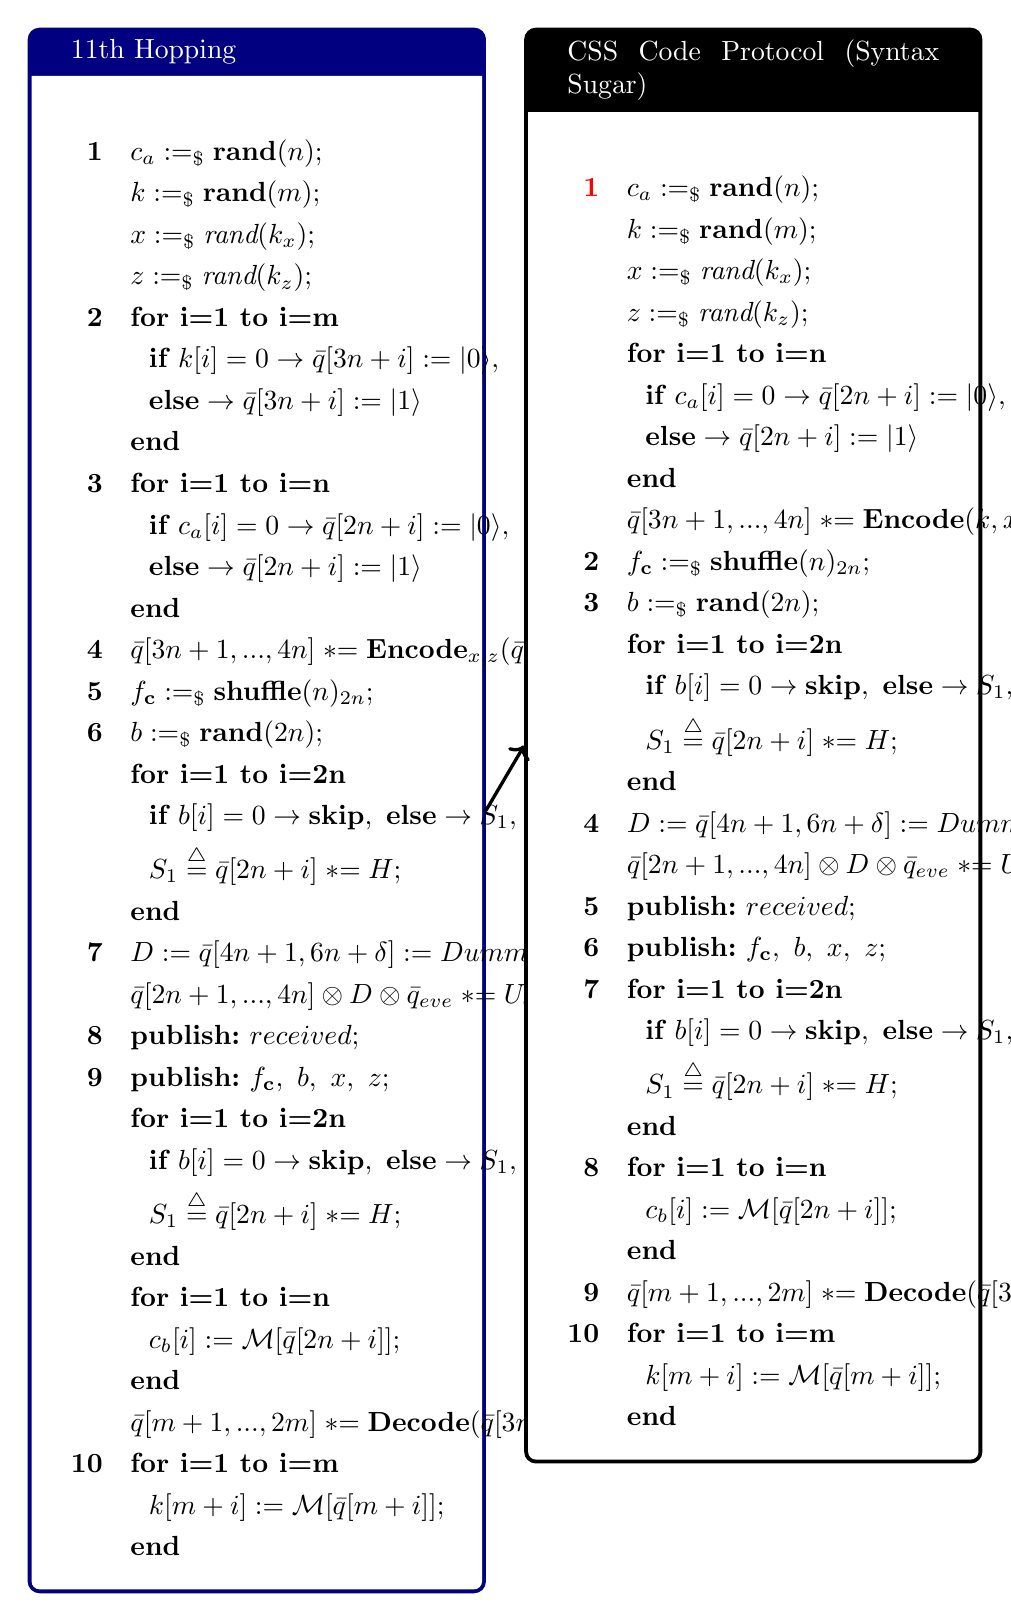
\begin{tikzpicture}[remember picture]

% Left box
\node[anchor=north west,inner sep=0pt,outer sep=0pt] (leftbox) at (0,0) {
\begin{minipage}[t]{0.48\textwidth}
\begin{tcolorbox}[colframe=blue!50!black, colback=white, title=11th Hopping, width=\textwidth]
\begin{align*}
    \textbf{{1}} \quad 
    & c_a :=_\$ \textbf{rand}(n); \\ 
    & k :=_\$ \textbf{rand}(m); \\ 
    & x :=_\$ \textit{rand}(k_x); \\
    & z :=_\$ \textit{rand}(k_z); \\ \textbf{{2}} \quad &\textbf{for~i=1~to~i=m}\\
    &~~ \textbf{if }  k[i] = 0 \rightarrow \bar{q}[3n+i] := |0\rangle,\\ &~~\textbf{else}   \rightarrow \bar{q}[3n+i] := |1\rangle\\
    &\textbf{end}\ \\
    \textbf{{3}} \quad 
    &\textbf{for~i=1~to~i=n}\\
    &~~ \textbf{if }  c_a[i] = 0 \rightarrow \bar{q}[2n+i] := |0\rangle,\\ &~~\textbf{else}   \rightarrow \bar{q}[2n+i] := |1\rangle\\
    &\textbf{end}\ \\
    \textbf{{4}} \quad 
    &\bar{q}[3n+1,...,4n]\asteq\textbf{Encode}_{x,z}(\bar{q}[3n+1,...,3n+m])\\
    \textbf{{5}} \quad & f_{\textbf{c}}:=_\$\textbf{shuffle}(n)_{2n}; \\
    \textbf{{6}} \quad & b :=_\$ \textbf{rand}(2n); \\
    &\textbf{for~i=1~to~i=2n}\\
    &~~ \textbf{if }  b[i] = 0 \rightarrow \textbf{skip},~\textbf{else}\rightarrow S_{1} ,\\
    &~~ S_{1}\stackrel{\triangle}{=}\bar{q}[2n+i] \asteq H ;\\
    &\textbf{end}\\
    \textbf{{7}} \quad & {D}:= \bar{q}[4n+1,6n+\delta]:=Dummy;\\     &\bar{q}[2n+1,...,4n]\otimes {D} \otimes \bar{q}_{eve} \asteq U_{\textbf{c}}(f_{\textbf{c}}); \\
    \textbf{{8}} \quad & \textbf{publish:}~ received;\\
    \textbf{{9}} \quad & \textbf{publish:}~ f_{\textbf{c}},~b, ~x,~ z;\\
    \quad & \textbf{for~i=1~to~i=2n}\\
    &~~ \textbf{if }  b[i] = 0 \rightarrow \textbf{skip},~\textbf{else}\rightarrow S_{1} ,\\
    &~~ S_{1}\stackrel{\triangle}{=}\bar{q}[2n+i] \asteq H ;\\
    &\textbf{end}\\
    \quad & \textbf{for~i=1~to~i=n}\\
    &~~ c_b[i]:= \mathcal{M} [\bar{q}[2n+i]];\\
    &\textbf{end}\\
    \quad & \bar{q}[m+1,...,2m]\asteq\textbf{Decode}(\bar{q}[3n+1,...,4n])\\
    \textbf{{10}} \quad 
    & \textbf{for~i=1~to~i=m}\\
    &~~ k[m+i]:= \mathcal{M} [\bar{q}[m+i]];\\
    &\textbf{end}
\end{align*}
\end{tcolorbox}
\end{minipage}
};

% Right box
\node[anchor=north west,inner sep=0pt,outer sep=0pt] (rightbox) at (0.52\textwidth,0) {
\begin{minipage}[t]{0.48\textwidth}
\begin{tcolorbox}[colframe=black!50!black, colback=white, title=CSS Code Protocol (Syntax Sugar), width=\textwidth]
\begin{align*}
    \textbf{\textcolor{red}{1}} \quad 
    & c_a :=_\$ \textbf{rand}(n); \\ 
    & k :=_\$ \textbf{rand}(m); \\ 
    & x :=_\$ \textit{rand}(k_x); \\
    & z :=_\$ \textit{rand}(k_z); \\
    \quad 
    &\textbf{for~i=1~to~i=n}\\
    &~~ \textbf{if }  c_a[i] = 0 \rightarrow \bar{q}[2n+i] := |0\rangle,\\ &~~\textbf{else}   \rightarrow \bar{q}[2n+i] := |1\rangle\\
    &\textbf{end}\ \\
    \quad 
    &\bar{q}[3n+1,...,4n]\asteq\textbf{Encode}(k,x,z)\\
    \textbf{{2}} \quad & f_{\textbf{c}}:=_\$\textbf{shuffle}(n)_{2n}; \\
    \textbf{{3}} \quad & b :=_\$ \textbf{rand}(2n); \\
    &\textbf{for~i=1~to~i=2n}\\
    &~~ \textbf{if }  b[i] = 0 \rightarrow \textbf{skip},~\textbf{else}\rightarrow S_{1} ,\\
    &~~ S_{1}\stackrel{\triangle}{=}\bar{q}[2n+i] \asteq H ;\\
    &\textbf{end}\\
    \textbf{{4}} \quad & {D}:= \bar{q}[4n+1,6n+\delta]:=Dummy;\\     &\bar{q}[2n+1,...,4n]\otimes {D} \otimes \bar{q}_{eve} \asteq U_{\textbf{c}}(f_{\textbf{c}}); \\
    \textbf{{5}} \quad & \textbf{publish:}~ received;\\
    \textbf{{6}} \quad & \textbf{publish:}~ f_{\textbf{c}},~b,~x,~z;\\
    \textbf{{7}} 
    \quad & \textbf{for~i=1~to~i=2n}\\
    &~~ \textbf{if }  b[i] = 0 \rightarrow \textbf{skip},~\textbf{else}\rightarrow S_{1} ,\\
    &~~ S_{1}\stackrel{\triangle}{=}\bar{q}[2n+i] \asteq H ;\\
    &\textbf{end}\\
    \textbf{{8}} 
    \quad & \textbf{for~i=1~to~i=n}\\
    &~~ c_b[i]:= \mathcal{M} [\bar{q}[2n+i]];\\
    &\textbf{end}\\
    \textbf{{9}} 
    \quad & \bar{q}[m+1,...,2m]\asteq\textbf{Decode}(\bar{q}[3n+1,...,4n])\\
    \textbf{{10}} \quad 
    & \textbf{for~i=1~to~i=m}\\
    &~~ k[m+i]:= \mathcal{M} [\bar{q}[m+i]];\\
    &\textbf{end}
\end{align*}
\end{tcolorbox}
\end{minipage}
};

% Draw arrow between boxes
\draw[->, very thick] (leftbox.east) -- node[above]{} (rightbox.west);

\end{tikzpicture}
% MOVE:  \section{Game Hoppings} here
% \subsection{Game Hopping between Lo-Chau Protocol and CSS Code Protocol}
% all tikzpicture / tcolorbox here

\paragraph{CSS-specific proof obligations for the Lo--Chau to CSS-code reduction.}

All CSS-specific obligations in this subsection are discharged by
Theorem~\ref{thm:css-correction-interface}. Hopping 7 uses the
purification-to-QEC interface and CSS syndrome correctness. Hopping 8 uses the
derived rule package \(\textsc{CSSSyn-Zero}\), because the inserted syndrome
ancillas and syndrome outputs satisfy
\[
\operatorname{Readout}((a_Z,a_X);(e_Z,e_X)).
\]
The later correction and decoding steps use the fixed CSS correction
correctness assumptions from Appendix~\ref{app:css-correction}.

\newpage
\subsection{CSS Code Protocol to BB84 Protocol}


\noindent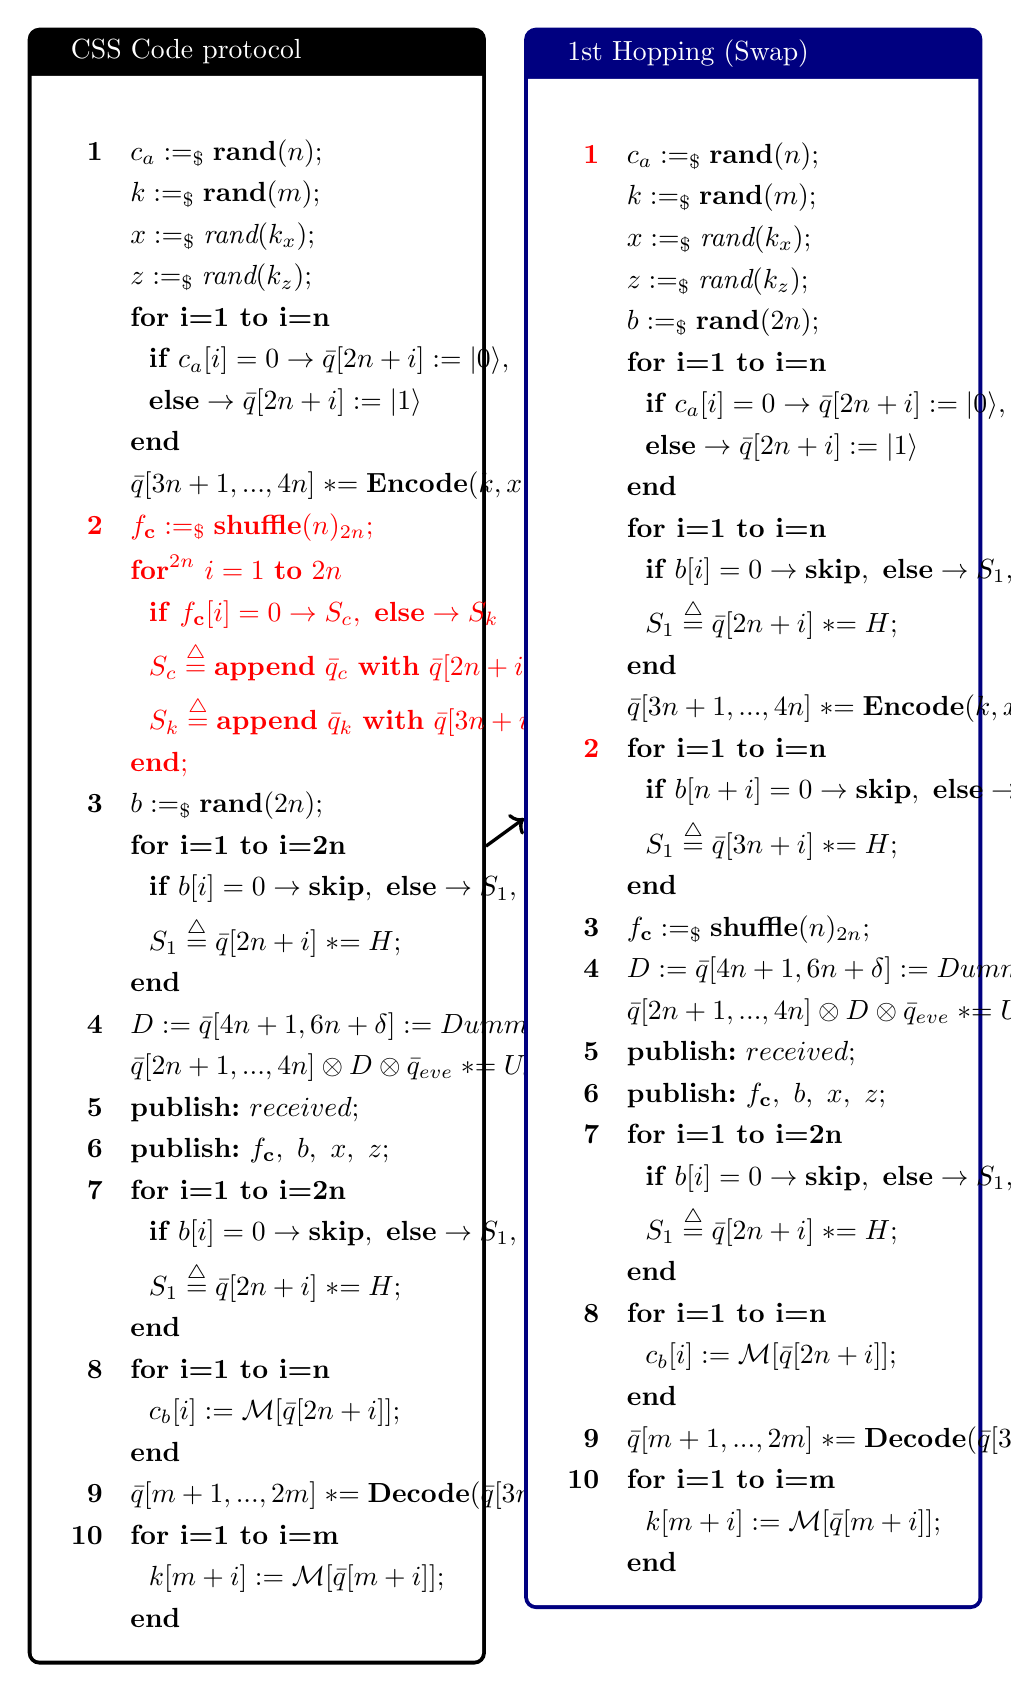
\begin{tikzpicture}[remember picture]

% Left box
\node[anchor=north west,inner sep=0pt,outer sep=0pt] (leftbox) at (0,0) {
\begin{minipage}[t]{0.48\textwidth}
\begin{tcolorbox}[colframe=black!50!black, colback=white, title=CSS Code protocol, width=\textwidth]
\begin{align*}
    \textbf{{1}} \quad 
    & c_a :=_\$ \textbf{rand}(n); \\ 
    & k :=_\$ \textbf{rand}(m); \\ 
    & x :=_\$ \textit{rand}(k_x); \\
    & z :=_\$ \textit{rand}(k_z); \\
    \quad 
    &\textbf{for~i=1~to~i=n}\\
    &~~ \textbf{if }  c_a[i] = 0 \rightarrow \bar{q}[2n+i] := |0\rangle,\\ &~~\textbf{else}   \rightarrow \bar{q}[2n+i] := |1\rangle\\
    &\textbf{end}\ \\
    \quad 
    &\bar{q}[3n+1,...,4n]\asteq\textbf{Encode}(k,x,z)\\
    \textbf{\textcolor{red}{2}} \quad
    & \textcolor{red}{f_{\textbf c}:=_\$\textbf{shuffle}(n)_{2n};}\\
    &\textcolor{red}{\mathbf{for}^{2n}\ i=1\ \mathbf{to}\ 2n}\\
    &~~ \textcolor{red}{\mathbf{if}\ f_{\textbf c}[i]=0\rightarrow S_c,\ 
    \mathbf{else}\rightarrow S_k}\\
    &~~ \textcolor{red}{S_c\stackrel{\triangle}{=}
    \mathbf{append}\ \bar q_{c}\ \mathbf{with}\
    \bar q[2n+i]}\\
    &~~ \textcolor{red}{S_k\stackrel{\triangle}{=}
    \mathbf{append}\ \bar q_{k}\ \mathbf{with}\
    \bar q[3n+i]}\\
    &\textcolor{red}{\mathbf{end};}\\
    \textbf{{3}} \quad & b :=_\$ \textbf{rand}(2n); \\
    &\textbf{for~i=1~to~i=2n}\\
    &~~ \textbf{if }  b[i] = 0 \rightarrow \textbf{skip},~\textbf{else}\rightarrow S_{1} ,\\
    &~~ S_{1}\stackrel{\triangle}{=}\bar{q}[2n+i] \asteq H ;\\
    &\textbf{end}\\
    \textbf{{4}} \quad & {D}:= \bar{q}[4n+1,6n+\delta]:=Dummy;\\     &\bar{q}[2n+1,...,4n]\otimes {D} \otimes \bar{q}_{eve} \asteq U_{\textbf{c}}(f_{\textbf{c}}); \\
    \textbf{{5}} \quad & \textbf{publish:}~ received;\\
    \textbf{{6}} \quad & \textbf{publish:}~ f_{\textbf{c}},~b,~x,~z;\\
    \textbf{{7}} 
    \quad & \textbf{for~i=1~to~i=2n}\\
    &~~ \textbf{if }  b[i] = 0 \rightarrow \textbf{skip},~\textbf{else}\rightarrow S_{1} ,\\
    &~~ S_{1}\stackrel{\triangle}{=}\bar{q}[2n+i] \asteq H ;\\
    &\textbf{end}\\
    \textbf{{8}} 
    \quad & \textbf{for~i=1~to~i=n}\\
    &~~ c_b[i]:= \mathcal{M} [\bar{q}[2n+i]];\\
    &\textbf{end}\\
    \textbf{{9}} 
    \quad & \bar{q}[m+1,...,2m]\asteq\textbf{Decode}(\bar{q}[3n+1,...,4n])\\
    \textbf{{10}} \quad 
    & \textbf{for~i=1~to~i=m}\\
    &~~ k[m+i]:= \mathcal{M} [\bar{q}[m+i]];\\
    &\textbf{end}
\end{align*}
\end{tcolorbox}
\end{minipage}
};

% Right box
\node[anchor=north west,inner sep=0pt,outer sep=0pt] (rightbox) at (0.52\textwidth,0) {
\begin{minipage}[t]{0.48\textwidth}
\begin{tcolorbox}[colframe=blue!50!black, colback=white, title=1st Hopping (Swap), width=\textwidth]
\begin{align*}
    \textbf{\textcolor{red}{1}} \quad 
    & c_a :=_\$ \textbf{rand}(n); \\ 
    & k :=_\$ \textbf{rand}(m); \\ 
    & x :=_\$ \textit{rand}(k_x); \\
    & z :=_\$ \textit{rand}(k_z); \\
    & b :=_\$ \textbf{rand}(2n); \\
    \quad 
    &\textbf{for~i=1~to~i=n}\\
    &~~ \textbf{if }  c_a[i] = 0 \rightarrow \bar{q}[2n+i] := |0\rangle,\\ &~~\textbf{else}   \rightarrow \bar{q}[2n+i] := |1\rangle\\
    &\textbf{end}\ \\
    \quad 
    &\textbf{for~i=1~to~i=n}\\
    &~~ \textbf{if }  b[i] = 0 \rightarrow \textbf{skip},~\textbf{else}\rightarrow S_{1} ,\\
    &~~ S_{1}\stackrel{\triangle}{=}\bar{q}[2n+i] \asteq H ;\\
    &\textbf{end}\\
    &\bar{q}[3n+1,...,4n]\asteq\textbf{Encode}(k,x,z)\\
    \textbf{\textcolor{red}{2}} \quad 
    &\textbf{for~i=1~to~i=n}\\
    &~~ \textbf{if }  b[n+i] = 0 \rightarrow \textbf{skip},~\textbf{else}\rightarrow S_{1} ,\\
    &~~ S_{1}\stackrel{\triangle}{=}\bar{q}[3n+i] \asteq H ;\\
    &\textbf{end}\\
    \textbf{{3}} \quad & f_{\textbf{c}}:=_\$\textbf{shuffle}(n)_{2n}; \\
    \textbf{{4}} \quad & {D}:= \bar{q}[4n+1,6n+\delta]:=Dummy;\\     &\bar{q}[2n+1,...,4n]\otimes {D} \otimes \bar{q}_{eve} \asteq U_{\textbf{c}}(f_{\textbf{c}}); \\
    \textbf{{5}} \quad & \textbf{publish:}~ received;\\
    \textbf{{6}} \quad & \textbf{publish:}~ f_{\textbf{c}},~b,~x,~z;\\
    \textbf{{7}} 
    \quad & \textbf{for~i=1~to~i=2n}\\
    &~~ \textbf{if }  b[i] = 0 \rightarrow \textbf{skip},~\textbf{else}\rightarrow S_{1} ,\\
    &~~ S_{1}\stackrel{\triangle}{=}\bar{q}[2n+i] \asteq H ;\\
    &\textbf{end}\\
    \textbf{{8}} 
    \quad & \textbf{for~i=1~to~i=n}\\
    &~~ c_b[i]:= \mathcal{M} [\bar{q}[2n+i]];\\
    &\textbf{end}\\
    \textbf{{9}} 
    \quad & \bar{q}[m+1,...,2m]\asteq\textbf{Decode}(\bar{q}[3n+1,...,4n])\\
    \textbf{{10}} \quad 
    & \textbf{for~i=1~to~i=m}\\
    &~~ k[m+i]:= \mathcal{M} [\bar{q}[m+i]];\\
    &\textbf{end}
\end{align*}
\end{tcolorbox}
\end{minipage}
};

% Draw arrow between boxes
\draw[->, very thick] (leftbox.east) -- node[above]{} (rightbox.west);

\end{tikzpicture}
\newpage
    
\noindent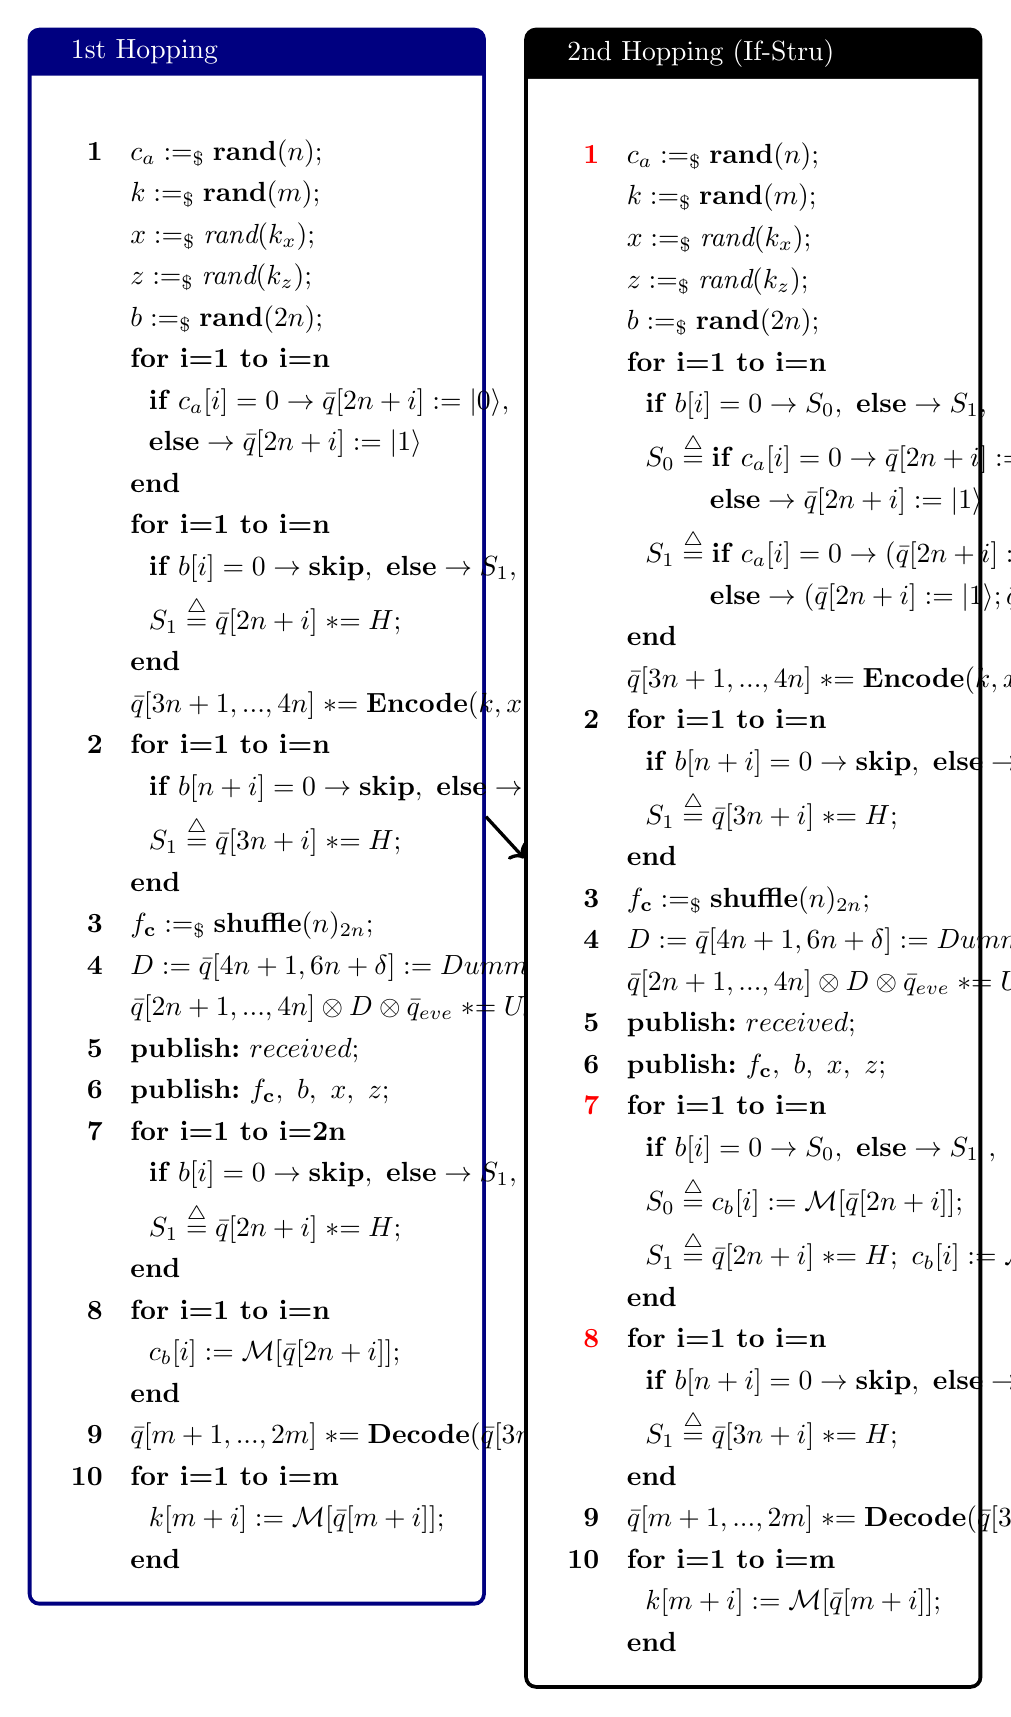
\begin{tikzpicture}[remember picture]

% Left box
\node[anchor=north west,inner sep=0pt,outer sep=0pt] (leftbox) at (0,0) {
\begin{minipage}[t]{0.48\textwidth}
\begin{tcolorbox}[colframe=blue!50!black, colback=white, title=1st Hopping, width=\textwidth]
\begin{align*}
    \textbf{{1}} \quad 
    & c_a :=_\$ \textbf{rand}(n); \\ 
    & k :=_\$ \textbf{rand}(m); \\ 
    & x :=_\$ \textit{rand}(k_x); \\
    & z :=_\$ \textit{rand}(k_z); \\
    & b :=_\$ \textbf{rand}(2n); \\
    \quad 
    &\textbf{for~i=1~to~i=n}\\
    &~~ \textbf{if }  c_a[i] = 0 \rightarrow \bar{q}[2n+i] := |0\rangle,\\ &~~\textbf{else}   \rightarrow \bar{q}[2n+i] := |1\rangle\\
    &\textbf{end}\ \\
    &\textbf{for~i=1~to~i=n}\\
    &~~ \textbf{if }  b[i] = 0 \rightarrow \textbf{skip},~\textbf{else}\rightarrow S_{1} ,\\
    &~~ S_{1}\stackrel{\triangle}{=}\bar{q}[2n+i] \asteq H ;\\
    &\textbf{end}\\
    \quad 
    &\bar{q}[3n+1,...,4n]\asteq\textbf{Encode}(k,x,z)\\
    \textbf{{2}} \quad 
    &\textbf{for~i=1~to~i=n}\\
    &~~ \textbf{if }  b[n+i] = 0 \rightarrow \textbf{skip},~\textbf{else}\rightarrow S_{1},\\
    &~~ S_{1}\stackrel{\triangle}{=}\bar{q}[3n+i] \asteq H ;\\
    &\textbf{end}\\
    \textbf{{3}} \quad & f_{\textbf{c}}:=_\$\textbf{shuffle}(n)_{2n}; \\
    \textbf{{4}} \quad & {D}:= \bar{q}[4n+1,6n+\delta]:=Dummy;\\     &\bar{q}[2n+1,...,4n]\otimes {D} \otimes \bar{q}_{eve} \asteq U_{\textbf{c}}(f_{\textbf{c}}); \\
    \textbf{{5}} \quad & \textbf{publish:}~ received;\\
    \textbf{{6}} \quad & \textbf{publish:}~ f_{\textbf{c}},~b,~x,~z;\\
    \textbf{{7}} 
    \quad & \textbf{for~i=1~to~i=2n}\\
    &~~ \textbf{if }  b[i] = 0 \rightarrow \textbf{skip},~\textbf{else}\rightarrow S_{1} ,\\
    &~~ S_{1}\stackrel{\triangle}{=}\bar{q}[2n+i] \asteq H ;\\
    &\textbf{end}\\
    \textbf{{8}} 
    \quad & \textbf{for~i=1~to~i=n}\\
    &~~ c_b[i]:= \mathcal{M} [\bar{q}[2n+i]];\\
    &\textbf{end}\\
    \textbf{{9}} 
    \quad & \bar{q}[m+1,...,2m]\asteq\textbf{Decode}(\bar{q}[3n+1,...,4n])\\
    \textbf{{10}} \quad 
    & \textbf{for~i=1~to~i=m}\\
    &~~ k[m+i]:= \mathcal{M} [\bar{q}[m+i]];\\
    &\textbf{end}
\end{align*}
\end{tcolorbox}
\end{minipage}
};

% Right box
\node[anchor=north west,inner sep=0pt,outer sep=0pt] (rightbox) at (0.52\textwidth,0) {
\begin{minipage}[t]{0.48\textwidth}
\begin{tcolorbox}[colframe=black!50!black, colback=white, title=2nd Hopping (If-Stru), width=\textwidth]
\begin{align*}
    \textbf{\textcolor{red}{1}} \quad 
    & c_a :=_\$ \textbf{rand}(n); \\ 
    & k :=_\$ \textbf{rand}(m); \\ 
    & x :=_\$ \textit{rand}(k_x); \\
    & z :=_\$ \textit{rand}(k_z); \\
    & b :=_\$ \textbf{rand}(2n); \\
    \quad 
    &\textbf{for~i=1~to~i=n}\\
    &~~ \textbf{if }  b[i] = 0 \rightarrow S_{0},~\textbf{else}\rightarrow S_{1} ,\\
    &~~ S_{0}\stackrel{\triangle}{=}\textbf{if }  c_a[i] = 0 \rightarrow \bar{q}[2n+i] := |0\rangle,\\ &~~~~~~~~~\textbf{else}   \rightarrow \bar{q}[2n+i] := |1\rangle\\
    &~~ S_{1}\stackrel{\triangle}{=}\textbf{if }  c_a[i] = 0 \rightarrow (\bar{q}[2n+i] := |0\rangle;\bar{q}[2n+i]\asteq H),\\ &~~~~~~~~~\textbf{else}   \rightarrow (\bar{q}[2n+i] := |1\rangle;\bar{q}[2n+i]\asteq H)\\
    &\textbf{end}\\\quad 
    &\bar{q}[3n+1,...,4n]\asteq\textbf{Encode}(k,x,z)\\
    \textbf{{2}} \quad 
    &\textbf{for~i=1~to~i=n}\\
    &~~ \textbf{if }  b[n+i] = 0 \rightarrow \textbf{skip},~\textbf{else}\rightarrow S_{1} ,\\
    &~~ S_{1}\stackrel{\triangle}{=}\bar{q}[3n+i] \asteq H ;\\
    &\textbf{end}\\
    \textbf{{3}} \quad & f_{\textbf{c}}:=_\$\textbf{shuffle}(n)_{2n}; \\
    \textbf{{4}} \quad & {D}:= \bar{q}[4n+1,6n+\delta]:=Dummy;\\     &\bar{q}[2n+1,...,4n]\otimes {D} \otimes \bar{q}_{eve} \asteq U_{\textbf{c}}(f_{\textbf{c}}); \\
    \textbf{{5}} \quad & \textbf{publish:}~ received;\\
    \textbf{{6}} \quad & \textbf{publish:}~ f_{\textbf{c}},~b,~x,~z;\\
    \textbf{\textcolor{red}{7}} 
    \quad 
    &\textbf{for~i=1~to~i=n}\\
    &~~ \textbf{if }  b[i] = 0 \rightarrow S_{0},~\textbf{else}\rightarrow S_{1}~,\\
    &~~ S_{0}\stackrel{\triangle}{=}c_b[i]:= \mathcal{M}[\bar{q}[2n+i]];\\
    &~~ S_{1}\stackrel{\triangle}{=}\bar{q}[2n+i]\asteq H;~c_b[i]:= \mathcal{M}[\bar{q}[2n+i]];\\
    &\textbf{end}\\
    \textbf{\textcolor{red}{8}}\quad 
    &\textbf{for~i=1~to~i=n}\\
    &~~ \textbf{if }  b[n+i] = 0 \rightarrow \textbf{skip},~\textbf{else}\rightarrow S_{1} ,\\
    &~~ S_{1}\stackrel{\triangle}{=}\bar{q}[3n+i] \asteq H ;\\
    &\textbf{end}\\
    \textbf{{9}} 
    \quad & \bar{q}[m+1,...,2m]\asteq\textbf{Decode}(\bar{q}[3n+1,...,4n])\\
    \textbf{{10}} \quad 
    & \textbf{for~i=1~to~i=m}\\
    &~~ k[m+i]:= \mathcal{M} [\bar{q}[m+i]];\\
    &\textbf{end}
\end{align*}
\end{tcolorbox}
\end{minipage}
};

% Draw arrow between boxes
\draw[->, very thick] (leftbox.east) -- node[above]{} (rightbox.west);

\end{tikzpicture}
\newpage

\noindent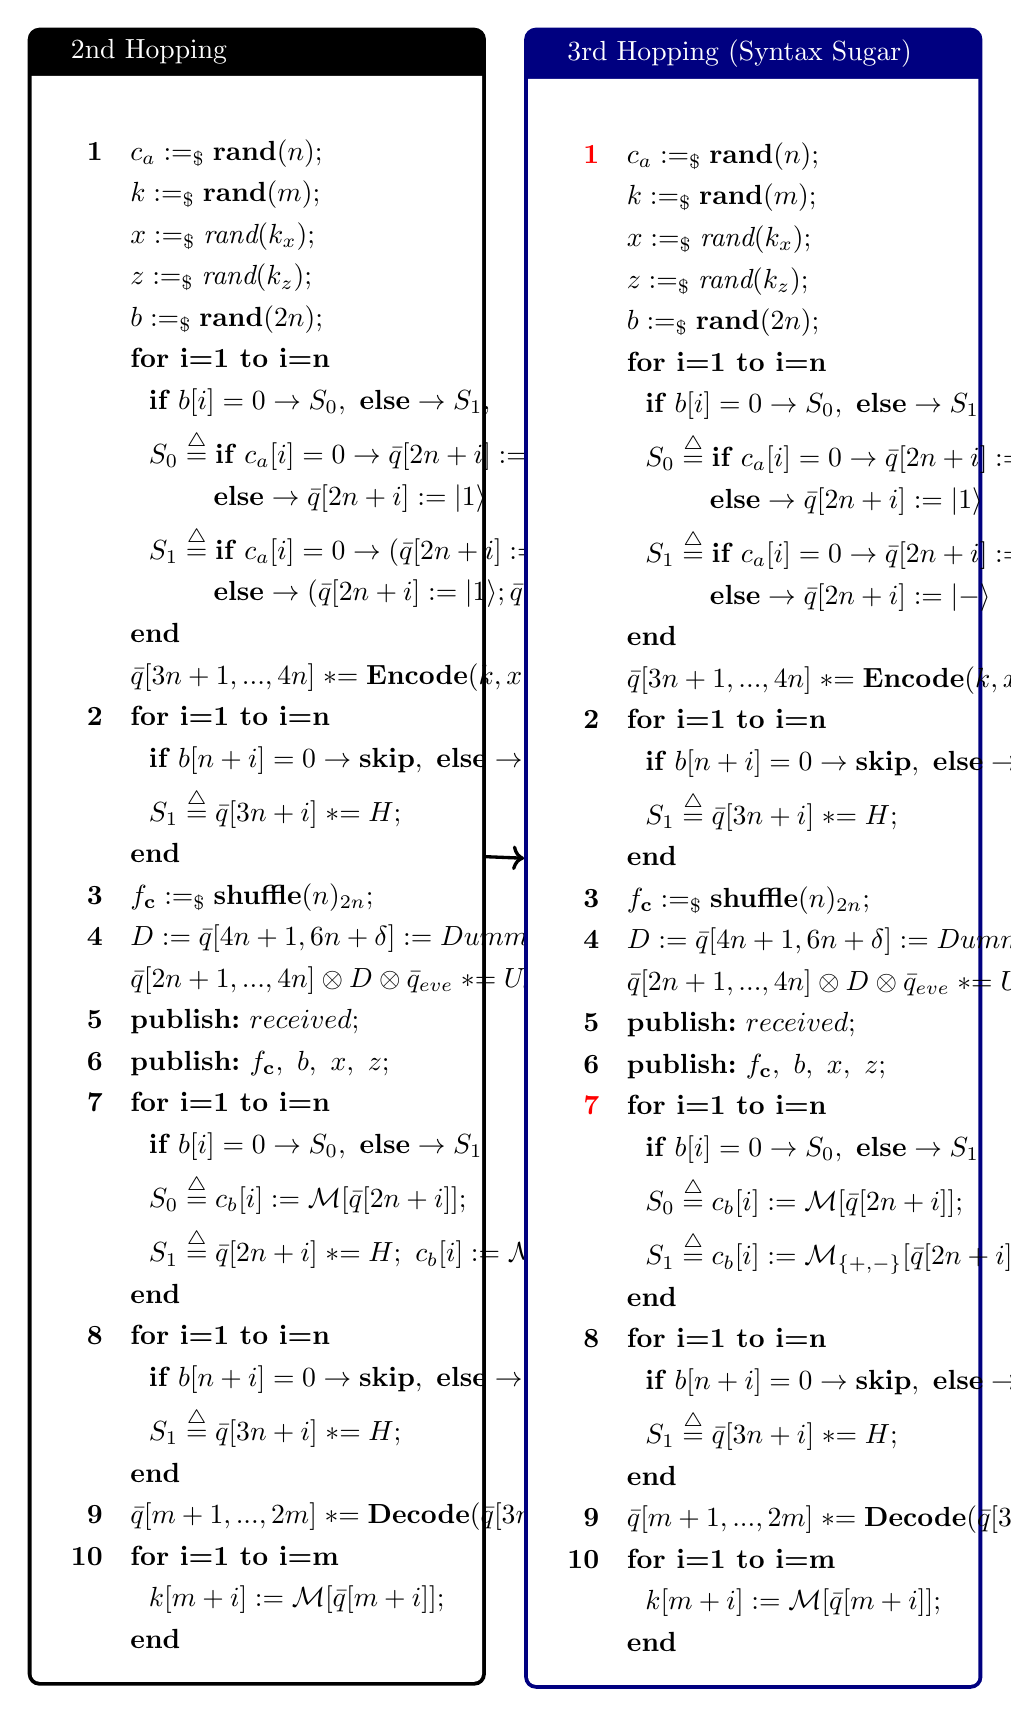
\begin{tikzpicture}[remember picture]

% Left box
\node[anchor=north west,inner sep=0pt,outer sep=0pt] (leftbox) at (0,0) {
\begin{minipage}[t]{0.48\textwidth}
\begin{tcolorbox}[colframe=black!50!black, colback=white, title=2nd Hopping, width=\textwidth]
\begin{align*}
    \textbf{{1}} \quad 
    & c_a :=_\$ \textbf{rand}(n); \\ 
    & k :=_\$ \textbf{rand}(m); \\ 
    & x :=_\$ \textit{rand}(k_x); \\
    & z :=_\$ \textit{rand}(k_z); \\
    & b :=_\$ \textbf{rand}(2n); \\
    \quad 
    &\textbf{for~i=1~to~i=n}\\
    &~~ \textbf{if }  b[i] = 0 \rightarrow S_{0},~\textbf{else}\rightarrow S_{1} ,\\
    &~~ S_{0}\stackrel{\triangle}{=}\textbf{if }  c_a[i] = 0 \rightarrow \bar{q}[2n+i] := |0\rangle,\\ &~~~~~~~~~\textbf{else}   \rightarrow \bar{q}[2n+i] := |1\rangle\\
    &~~ S_{1}\stackrel{\triangle}{=}\textbf{if }  c_a[i] = 0 \rightarrow (\bar{q}[2n+i] := |0\rangle;\bar{q}[2n+i]\asteq H),\\ &~~~~~~~~~\textbf{else}   \rightarrow (\bar{q}[2n+i] := |1\rangle;\bar{q}[2n+i]\asteq H)\\
    &\textbf{end}\\\quad 
    &\bar{q}[3n+1,...,4n]\asteq\textbf{Encode}(k,x,z)\\
    \textbf{{2}} \quad 
    &\textbf{for~i=1~to~i=n}\\
    &~~ \textbf{if }  b[n+i] = 0 \rightarrow \textbf{skip},~\textbf{else}\rightarrow S_{1} ,\\
    &~~ S_{1}\stackrel{\triangle}{=}\bar{q}[3n+i] \asteq H ;\\
    &\textbf{end}\\
    \textbf{{3}} \quad & f_{\textbf{c}}:=_\$\textbf{shuffle}(n)_{2n}; \\
    \textbf{{4}} \quad & {D}:= \bar{q}[4n+1,6n+\delta]:=Dummy;\\     &\bar{q}[2n+1,...,4n]\otimes {D} \otimes \bar{q}_{eve} \asteq U_{\textbf{c}}(f_{\textbf{c}}); \\
    \textbf{{5}} \quad & \textbf{publish:}~ received;\\
    \textbf{{6}} \quad & \textbf{publish:}~ f_{\textbf{c}},~b,~x,~z;\\
    \textbf{{7}} 
    \quad 
    &\textbf{for~i=1~to~i=n}\\
    &~~ \textbf{if }  b[i] = 0 \rightarrow S_{0},~\textbf{else}\rightarrow S_{1}\\
    &~~ S_{0}\stackrel{\triangle}{=}c_b[i]:= \mathcal{M}[\bar{q}[2n+i]];\\
    &~~ S_{1}\stackrel{\triangle}{=}\bar{q}[2n+i]\asteq H;~c_b[i]:= \mathcal{M}[\bar{q}[2n+i]];\\
    &\textbf{end}\\
    \textbf{{8}}\quad 
    &\textbf{for~i=1~to~i=n}\\
    &~~ \textbf{if }  b[n+i] = 0 \rightarrow \textbf{skip},~\textbf{else}\rightarrow S_{1} ,\\
    &~~ S_{1}\stackrel{\triangle}{=}\bar{q}[3n+i] \asteq H ;\\
    &\textbf{end}\\
    \textbf{{9}} 
    \quad & \bar{q}[m+1,...,2m]\asteq\textbf{Decode}(\bar{q}[3n+1,...,4n])\\
    \textbf{{10}} \quad 
    & \textbf{for~i=1~to~i=m}\\
    &~~ k[m+i]:= \mathcal{M} [\bar{q}[m+i]];\\
    &\textbf{end}
\end{align*}
\end{tcolorbox}
\end{minipage}
};

% Right box
\node[anchor=north west,inner sep=0pt,outer sep=0pt] (rightbox) at (0.52\textwidth,0) {
\begin{minipage}[t]{0.48\textwidth}
\begin{tcolorbox}[colframe=blue!50!black, colback=white, title=3rd Hopping (Syntax Sugar), width=\textwidth]
\begin{align*}
    \textbf{\textcolor{red}{1}} \quad 
    & c_a :=_\$ \textbf{rand}(n); \\ 
    & k :=_\$ \textbf{rand}(m); \\ 
    & x :=_\$ \textit{rand}(k_x); \\
    & z :=_\$ \textit{rand}(k_z); \\
    & b :=_\$ \textbf{rand}(2n); \\
    \quad 
    &\textbf{for~i=1~to~i=n}\\
    &~~ \textbf{if }  b[i] = 0 \rightarrow S_{0},~\textbf{else}\rightarrow S_{1}\\
    &~~ S_{0}\stackrel{\triangle}{=}\textbf{if }  c_a[i] = 0 \rightarrow \bar{q}[2n+i] := |0\rangle,\\ &~~~~~~~~~\textbf{else}   \rightarrow \bar{q}[2n+i] := |1\rangle\\
    &~~ S_{1}\stackrel{\triangle}{=}\textbf{if }  c_a[i] = 0 \rightarrow \bar{q}[2n+i] := |+\rangle,\\ &~~~~~~~~~\textbf{else}   \rightarrow \bar{q}[2n+i] := |-\rangle\\
    &\textbf{end}\\\quad 
    &\bar{q}[3n+1,...,4n]\asteq\textbf{Encode}(k,x,z)\\
    \textbf{{2}} \quad 
    &\textbf{for~i=1~to~i=n}\\
    &~~ \textbf{if }  b[n+i] = 0 \rightarrow \textbf{skip},~\textbf{else}\rightarrow S_{1} ,\\
    &~~ S_{1}\stackrel{\triangle}{=}\bar{q}[3n+i] \asteq H ;\\
    &\textbf{end}\\
    \textbf{{3}} \quad & f_{\textbf{c}}:=_\$\textbf{shuffle}(n)_{2n}; \\
    \textbf{{4}} \quad & {D}:= \bar{q}[4n+1,6n+\delta]:=Dummy;\\     &\bar{q}[2n+1,...,4n]\otimes {D} \otimes \bar{q}_{eve} \asteq U_{\textbf{c}}(f_{\textbf{c}}); \\
    \textbf{{5}} \quad & \textbf{publish:}~ received;\\
    \textbf{{6}} \quad & \textbf{publish:}~ f_{\textbf{c}},~b,~x,~z;\\
    \textbf{\textcolor{red}{7}} 
    \quad 
    &\textbf{for~i=1~to~i=n}\\
    &~~ \textbf{if }  b[i] = 0 \rightarrow S_{0},~\textbf{else}\rightarrow S_{1}\\
    &~~ S_{0}\stackrel{\triangle}{=}c_b[i]:= \mathcal{M} [\bar{q}[2n+i]];\\
    &~~ S_{1}\stackrel{\triangle}{=}c_b[i]:= \mathcal{M}_{\{+,-\}} [\bar{q}[2n+i]];\\
    &\textbf{end}\\
    \textbf{{8}}\quad 
    &\textbf{for~i=1~to~i=n}\\
    &~~ \textbf{if }  b[n+i] = 0 \rightarrow \textbf{skip},~\textbf{else}\rightarrow S_{1} ,\\
    &~~ S_{1}\stackrel{\triangle}{=}\bar{q}[3n+i] \asteq H ;\\
    &\textbf{end}\\
    \textbf{{9}} 
    \quad & \bar{q}[m+1,...,2m]\asteq\textbf{Decode}(\bar{q}[3n+1,...,4n])\\
    \textbf{{10}} \quad 
    & \textbf{for~i=1~to~i=m}\\
    &~~ k[m+i]:= \mathcal{M} [\bar{q}[m+i]];\\
    &\textbf{end}
\end{align*}
\end{tcolorbox}
\end{minipage}
};

% Draw arrow between boxes
\draw[->, very thick] (leftbox.east) -- node[above]{} (rightbox.west);

\end{tikzpicture}
\newpage


\noindent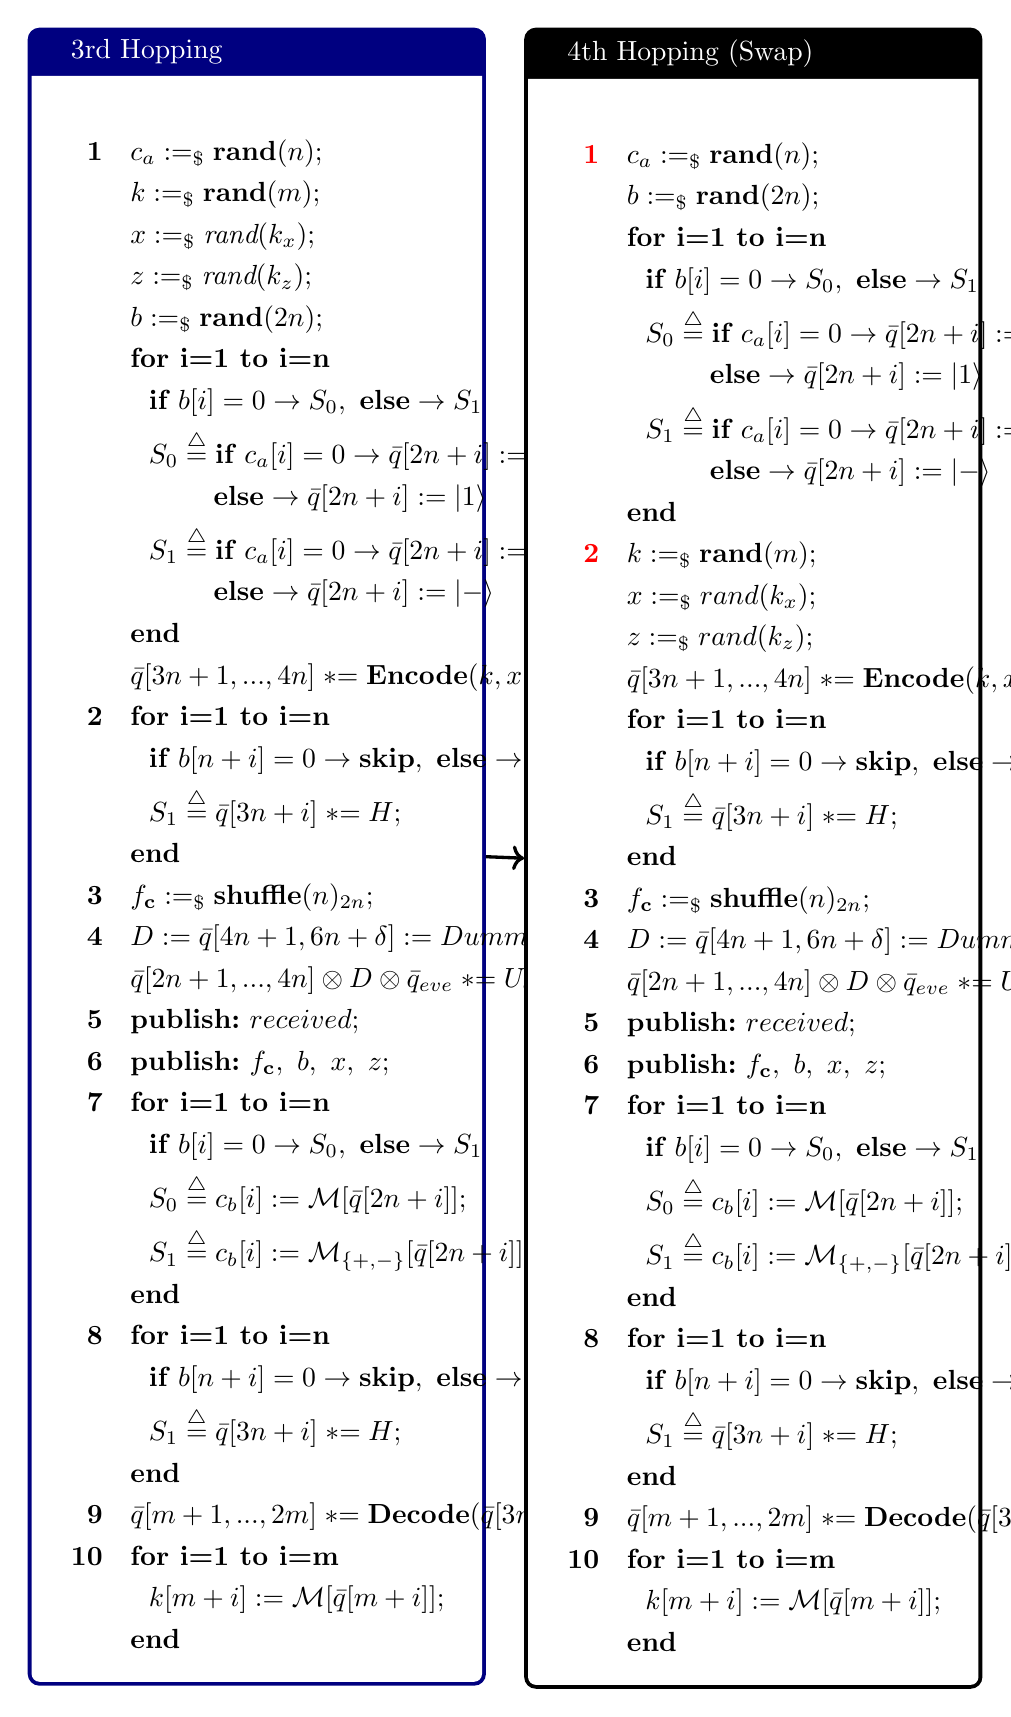
\begin{tikzpicture}[remember picture]

% Left box
\node[anchor=north west,inner sep=0pt,outer sep=0pt] (leftbox) at (0,0) {
\begin{minipage}[t]{0.48\textwidth}
\begin{tcolorbox}[colframe=blue!50!black, colback=white, title=3rd Hopping, width=\textwidth]
\begin{align*}
    \textbf{{1}} \quad 
    & c_a :=_\$ \textbf{rand}(n); \\ 
    & k :=_\$ \textbf{rand}(m); \\ 
    & x :=_\$ \textit{rand}(k_x); \\
    & z :=_\$ \textit{rand}(k_z); \\
    & b :=_\$ \textbf{rand}(2n); \\
    \quad 
    &\textbf{for~i=1~to~i=n}\\
    &~~ \textbf{if }  b[i] = 0 \rightarrow S_{0},~\textbf{else}\rightarrow S_{1}\\
    &~~ S_{0}\stackrel{\triangle}{=}\textbf{if }  c_a[i] = 0 \rightarrow \bar{q}[2n+i] := |0\rangle,\\ &~~~~~~~~~\textbf{else}   \rightarrow \bar{q}[2n+i] := |1\rangle\\
    &~~ S_{1}\stackrel{\triangle}{=}\textbf{if }  c_a[i] = 0 \rightarrow \bar{q}[2n+i] := |+\rangle,\\ &~~~~~~~~~\textbf{else}   \rightarrow \bar{q}[2n+i] := |-\rangle\\
    &\textbf{end}\\\quad 
    &\bar{q}[3n+1,...,4n]\asteq\textbf{Encode}(k,x,z)\\
    \textbf{{2}} \quad 
    &\textbf{for~i=1~to~i=n}\\
    &~~ \textbf{if }  b[n+i] = 0 \rightarrow \textbf{skip},~\textbf{else}\rightarrow S_{1} ,\\
    &~~ S_{1}\stackrel{\triangle}{=}\bar{q}[3n+i] \asteq H ;\\
    &\textbf{end}\\
    \textbf{{3}} \quad & f_{\textbf{c}}:=_\$\textbf{shuffle}(n)_{2n}; \\
    \textbf{{4}} \quad & {D}:= \bar{q}[4n+1,6n+\delta]:=Dummy;\\     &\bar{q}[2n+1,...,4n]\otimes {D} \otimes \bar{q}_{eve} \asteq U_{\textbf{c}}(f_{\textbf{c}}); \\
    \textbf{{5}} \quad & \textbf{publish:}~ received;\\
    \textbf{{6}} \quad & \textbf{publish:}~ f_{\textbf{c}},~b,~x,~z;\\
    \textbf{{7}} 
    \quad 
    &\textbf{for~i=1~to~i=n}\\
    &~~ \textbf{if }  b[i] = 0 \rightarrow S_{0},~\textbf{else}\rightarrow S_{1}\\
    &~~ S_{0}\stackrel{\triangle}{=}c_b[i]:= \mathcal{M} [\bar{q}[2n+i]];\\
    &~~ S_{1}\stackrel{\triangle}{=}c_b[i]:= \mathcal{M}_{\{+,-\}} [\bar{q}[2n+i]];\\
    &\textbf{end}\\
    \textbf{{8}}\quad 
    &\textbf{for~i=1~to~i=n}\\
    &~~ \textbf{if }  b[n+i] = 0 \rightarrow \textbf{skip},~\textbf{else}\rightarrow S_{1} ,\\
    &~~ S_{1}\stackrel{\triangle}{=}\bar{q}[3n+i] \asteq H ;\\
    &\textbf{end}\\
    \textbf{{9}} 
    \quad & \bar{q}[m+1,...,2m]\asteq\textbf{Decode}(\bar{q}[3n+1,...,4n])\\
    \textbf{{10}} \quad 
    & \textbf{for~i=1~to~i=m}\\
    &~~ k[m+i]:= \mathcal{M} [\bar{q}[m+i]];\\
    &\textbf{end}
\end{align*}
\end{tcolorbox}
\end{minipage}
};

% Right box
\node[anchor=north west,inner sep=0pt,outer sep=0pt] (rightbox) at (0.52\textwidth,0) {
\begin{minipage}[t]{0.48\textwidth}
\begin{tcolorbox}[colframe=black!50!black, colback=white, title=4th Hopping (Swap), width=\textwidth]
\begin{align*}
    \textbf{\textcolor{red}{1}} \quad 
    & c_a :=_\$ \textbf{rand}(n); \\ 
    & b :=_\$ \textbf{rand}(2n); \\
    &\textbf{for~i=1~to~i=n}\\
    &~~ \textbf{if }  b[i] = 0 \rightarrow S_{0},~\textbf{else}\rightarrow S_{1}\\
    &~~ S_{0}\stackrel{\triangle}{=}\textbf{if }  c_a[i] = 0 \rightarrow \bar{q}[2n+i] := |0\rangle,\\ &~~~~~~~~~\textbf{else}   \rightarrow \bar{q}[2n+i] := |1\rangle\\
    &~~ S_{1}\stackrel{\triangle}{=}\textbf{if }  c_a[i] = 0 \rightarrow \bar{q}[2n+i] := |+\rangle,\\ &~~~~~~~~~\textbf{else}   \rightarrow \bar{q}[2n+i] := |-\rangle\\
    &\textbf{end}\\
    \textbf{\textcolor{red}{2}}\quad 
    & k :=_\$ \textbf{rand}(m); \\
    & x :=_\$ {rand}(k_x); \\
    & z :=_\$ {rand}(k_z); \\
    &\bar{q}[3n+1,...,4n]\asteq\textbf{Encode}(k,x,z)\\
    &\textbf{for~i=1~to~i=n}\\
    &~~ \textbf{if }  b[n+i] = 0 \rightarrow \textbf{skip},~\textbf{else}\rightarrow S_{1} ,\\
    &~~ S_{1}\stackrel{\triangle}{=}\bar{q}[3n+i] \asteq H ;\\
    &\textbf{end}\\
    \textbf{{3}} \quad & f_{\textbf{c}}:=_\$\textbf{shuffle}(n)_{2n}; \\
    \textbf{{4}} \quad & {D}:= \bar{q}[4n+1,6n+\delta]:=Dummy;\\     &\bar{q}[2n+1,...,4n]\otimes {D} \otimes \bar{q}_{eve} \asteq U_{\textbf{c}}(f_{\textbf{c}}); \\
    \textbf{{5}} \quad & \textbf{publish:}~ received;\\
    \textbf{{6}} \quad & \textbf{publish:}~ f_{\textbf{c}},~b,~x,~z;\\
    \textbf{{7}} 
    \quad 
    &\textbf{for~i=1~to~i=n}\\
    &~~ \textbf{if }  b[i] = 0 \rightarrow S_{0},~\textbf{else}\rightarrow S_{1}\\
    &~~ S_{0}\stackrel{\triangle}{=}c_b[i]:= \mathcal{M} [\bar{q}[2n+i]];\\
    &~~ S_{1}\stackrel{\triangle}{=}c_b[i]:= \mathcal{M}_{\{+,-\}} [\bar{q}[2n+i]];\\
    &\textbf{end}\\
    \textbf{{8}}\quad 
    &\textbf{for~i=1~to~i=n}\\
    &~~ \textbf{if }  b[n+i] = 0 \rightarrow \textbf{skip},~\textbf{else}\rightarrow S_{1} ,\\
    &~~ S_{1}\stackrel{\triangle}{=}\bar{q}[3n+i] \asteq H ;\\
    &\textbf{end}\\
    \textbf{{9}} 
    \quad & \bar{q}[m+1,...,2m]\asteq\textbf{Decode}(\bar{q}[3n+1,...,4n])\\
    \textbf{{10}} \quad 
    & \textbf{for~i=1~to~i=m}\\
    &~~ k[m+i]:= \mathcal{M} [\bar{q}[m+i]];\\
    &\textbf{end}
\end{align*}
\end{tcolorbox}
\end{minipage}
};

% Draw arrow between boxes
\draw[->, very thick] (leftbox.east) -- node[above]{} (rightbox.west);

\end{tikzpicture}
\newpage

\noindent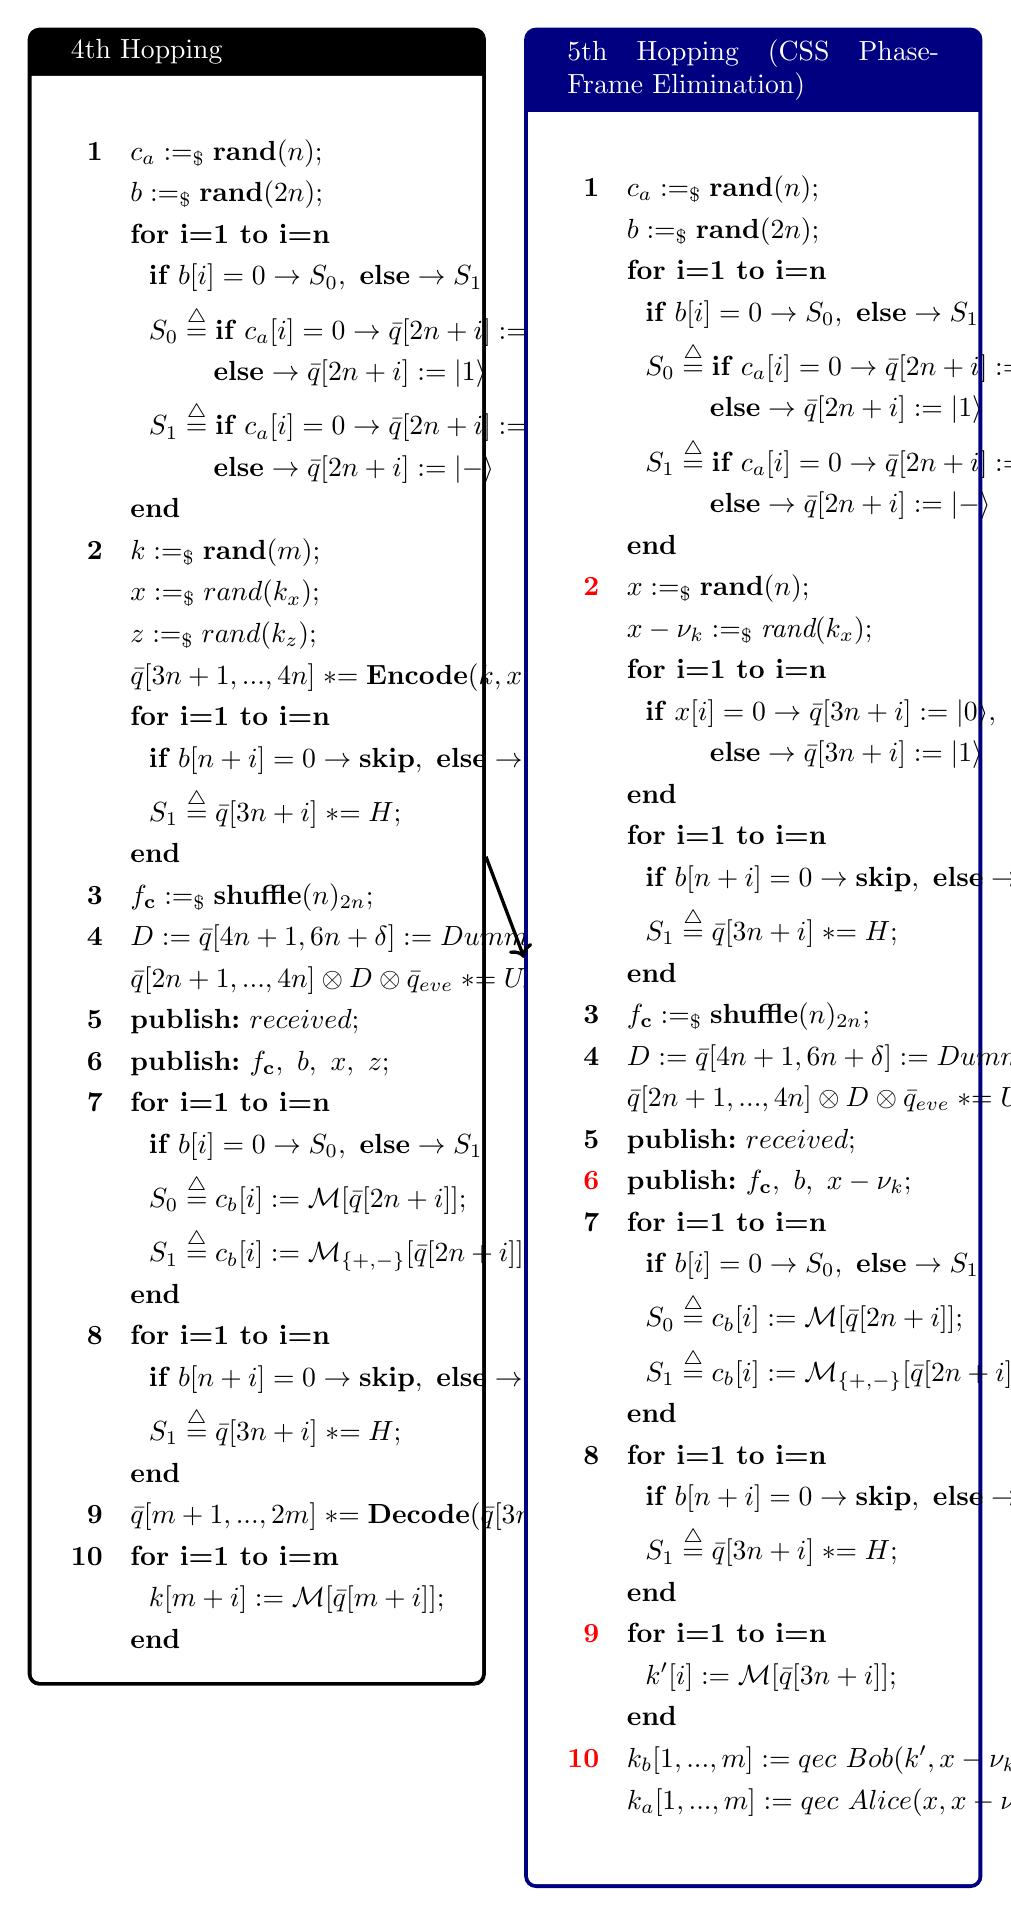
\begin{tikzpicture}[remember picture]

% Left box
\node[anchor=north west,inner sep=0pt,outer sep=0pt] (leftbox) at (0,0) {
\begin{minipage}[t]{0.48\textwidth}
\begin{tcolorbox}[colframe=black!50!black, colback=white, title=4th Hopping, width=\textwidth]
\begin{align*}
    \textbf{{1}} \quad 
    & c_a :=_\$ \textbf{rand}(n); \\ 
    & b :=_\$ \textbf{rand}(2n); \\
    &\textbf{for~i=1~to~i=n}\\
    &~~ \textbf{if }  b[i] = 0 \rightarrow S_{0},~\textbf{else}\rightarrow S_{1}\\
    &~~ S_{0}\stackrel{\triangle}{=}\textbf{if }  c_a[i] = 0 \rightarrow \bar{q}[2n+i] := |0\rangle,\\ &~~~~~~~~~\textbf{else}   \rightarrow \bar{q}[2n+i] := |1\rangle\\
    &~~ S_{1}\stackrel{\triangle}{=}\textbf{if }  c_a[i] = 0 \rightarrow \bar{q}[2n+i] := |+\rangle,\\ &~~~~~~~~~\textbf{else}   \rightarrow \bar{q}[2n+i] := |-\rangle\\
    &\textbf{end}\\
    \textbf{{2}}\quad 
    & k :=_\$ \textbf{rand}(m); \\
    & x :=_\$ {rand}(k_x); \\
    & z :=_\$ {rand}(k_z); \\
    &\bar{q}[3n+1,...,4n]\asteq\textbf{Encode}(k,x,z)\\
    &\textbf{for~i=1~to~i=n}\\
    &~~ \textbf{if }  b[n+i] = 0 \rightarrow \textbf{skip},~\textbf{else}\rightarrow S_{1} ,\\
    &~~ S_{1}\stackrel{\triangle}{=}\bar{q}[3n+i] \asteq H ;\\
    &\textbf{end}\\
    \textbf{{3}} \quad & f_{\textbf{c}}:=_\$\textbf{shuffle}(n)_{2n}; \\
    \textbf{{4}} \quad & {D}:= \bar{q}[4n+1,6n+\delta]:=Dummy;\\     &\bar{q}[2n+1,...,4n]\otimes {D} \otimes \bar{q}_{eve} \asteq U_{\textbf{c}}(f_{\textbf{c}}); \\
    \textbf{{5}} \quad & \textbf{publish:}~ received;\\
    \textbf{{6}} \quad & \textbf{publish:}~ f_{\textbf{c}},~b,~x,~z;\\
    \textbf{{7}} 
    \quad 
    &\textbf{for~i=1~to~i=n}\\
    &~~ \textbf{if }  b[i] = 0 \rightarrow S_{0},~\textbf{else}\rightarrow S_{1}\\
    &~~ S_{0}\stackrel{\triangle}{=}c_b[i]:= \mathcal{M} [\bar{q}[2n+i]];\\
    &~~ S_{1}\stackrel{\triangle}{=}c_b[i]:= \mathcal{M}_{\{+,-\}} [\bar{q}[2n+i]];\\
    &\textbf{end}\\
    \textbf{{8}}\quad 
    &\textbf{for~i=1~to~i=n}\\
    &~~ \textbf{if }  b[n+i] = 0 \rightarrow \textbf{skip},~\textbf{else}\rightarrow S_{1} ,\\
    &~~ S_{1}\stackrel{\triangle}{=}\bar{q}[3n+i] \asteq H ;\\
    &\textbf{end}\\
    \textbf{{9}} 
    \quad & \bar{q}[m+1,...,2m]\asteq\textbf{Decode}(\bar{q}[3n+1,...,4n])\\
    \textbf{{10}} \quad 
    & \textbf{for~i=1~to~i=m}\\
    &~~ k[m+i]:= \mathcal{M} [\bar{q}[m+i]];\\
    &\textbf{end}
\end{align*}
\end{tcolorbox}
\end{minipage}
};

% Right box
\node[anchor=north west,inner sep=0pt,outer sep=0pt] (rightbox) at (0.52\textwidth,0) {
\begin{minipage}[t]{0.48\textwidth}
\begin{tcolorbox}[colframe=blue!50!black, colback=white, title=5th Hopping (CSS Phase-Frame Elimination), width=\textwidth]
\begin{align*}
    \textbf{{1}} \quad 
    & c_a :=_\$ \textbf{rand}(n); \\ 
    & b :=_\$ \textbf{rand}(2n); \\
    \quad 
    &\textbf{for~i=1~to~i=n}\\
    &~~ \textbf{if }  b[i] = 0 \rightarrow S_{0},~\textbf{else}\rightarrow S_{1}\\
    &~~ S_{0}\stackrel{\triangle}{=}\textbf{if }  c_a[i] = 0 \rightarrow \bar{q}[2n+i] := |0\rangle,\\ &~~~~~~~~~\textbf{else}   \rightarrow \bar{q}[2n+i] := |1\rangle\\
    &~~ S_{1}\stackrel{\triangle}{=}\textbf{if }  c_a[i] = 0 \rightarrow \bar{q}[2n+i] := |+\rangle,\\ &~~~~~~~~~\textbf{else}   \rightarrow \bar{q}[2n+i] := |-\rangle\\
    &\textbf{end}\\
    \textbf{\textcolor{red}{2}}\quad 
    & x :=_\$ \textbf{rand}(n); \\
    & x-\nu_k :=_\$ \textit{rand}(k_x);\\
    &\textbf{for~i=1~to~i=n}\\
    &~~ \textbf{if }  x[i] = 0 \rightarrow \bar{q}[3n+i] := |0\rangle,\\ &~~~~~~~~~\textbf{else}   \rightarrow \bar{q}[3n+i] := |1\rangle\\
    &\textbf{end}\\
    &\textbf{for~i=1~to~i=n}\\
    &~~ \textbf{if }  b[n+i] = 0 \rightarrow \textbf{skip},~\textbf{else}\rightarrow S_{1} ,\\
    &~~ S_{1}\stackrel{\triangle}{=}\bar{q}[3n+i] \asteq H ;\\
    &\textbf{end}\\
    \textbf{{3}} \quad & f_{\textbf{c}}:=_\$\textbf{shuffle}(n)_{2n}; \\
    \textbf{{4}} \quad & {D}:= \bar{q}[4n+1,6n+\delta]:=Dummy;\\     &\bar{q}[2n+1,...,4n]\otimes {D} \otimes \bar{q}_{eve} \asteq U_{\textbf{c}}(f_{\textbf{c}}); \\
    \textbf{{5}} \quad & \textbf{publish:}~ received;\\
    \textbf{\textcolor{red}{6}} \quad & \textbf{publish:}~ f_{\textbf{c}},~b,~x-\nu_k;\\
    \textbf{{7}} 
    \quad 
    &\textbf{for~i=1~to~i=n}\\
    &~~ \textbf{if }  b[i] = 0 \rightarrow S_{0},~\textbf{else}\rightarrow S_{1}\\
    &~~ S_{0}\stackrel{\triangle}{=}c_b[i]:= \mathcal{M} [\bar{q}[2n+i]];\\
    &~~ S_{1}\stackrel{\triangle}{=}c_b[i]:= \mathcal{M}_{\{+,-\}} [\bar{q}[2n+i]];\\
    &\textbf{end}\\
    \textbf{{8}}\quad 
    &\textbf{for~i=1~to~i=n}\\
    &~~ \textbf{if }  b[n+i] = 0 \rightarrow \textbf{skip},~\textbf{else}\rightarrow S_{1} ,\\
    &~~ S_{1}\stackrel{\triangle}{=}\bar{q}[3n+i] \asteq H ;\\
    &\textbf{end}\\
    \textbf{\textcolor{red}{9}} \quad 
    &\textbf{for~i=1~to~i=n}\\
    &~~ k'[i]:= \mathcal{M} [\bar{q}[3n+i]];\\
    &\textbf{end}\\
    \textcolor{red}{\textbf{10}} \quad & k_b[1,...,m]:=qec~Bob(k',x-\nu_k)\\
    &k_a[1,...,m]:=qec~Alice(x,x-\nu_k)\\
\end{align*}
\end{tcolorbox}
\end{minipage}
};

% Draw arrow between boxes
\draw[->, very thick] (leftbox.east) -- node[above]{} (rightbox.west);

\end{tikzpicture}
\newpage

\noindent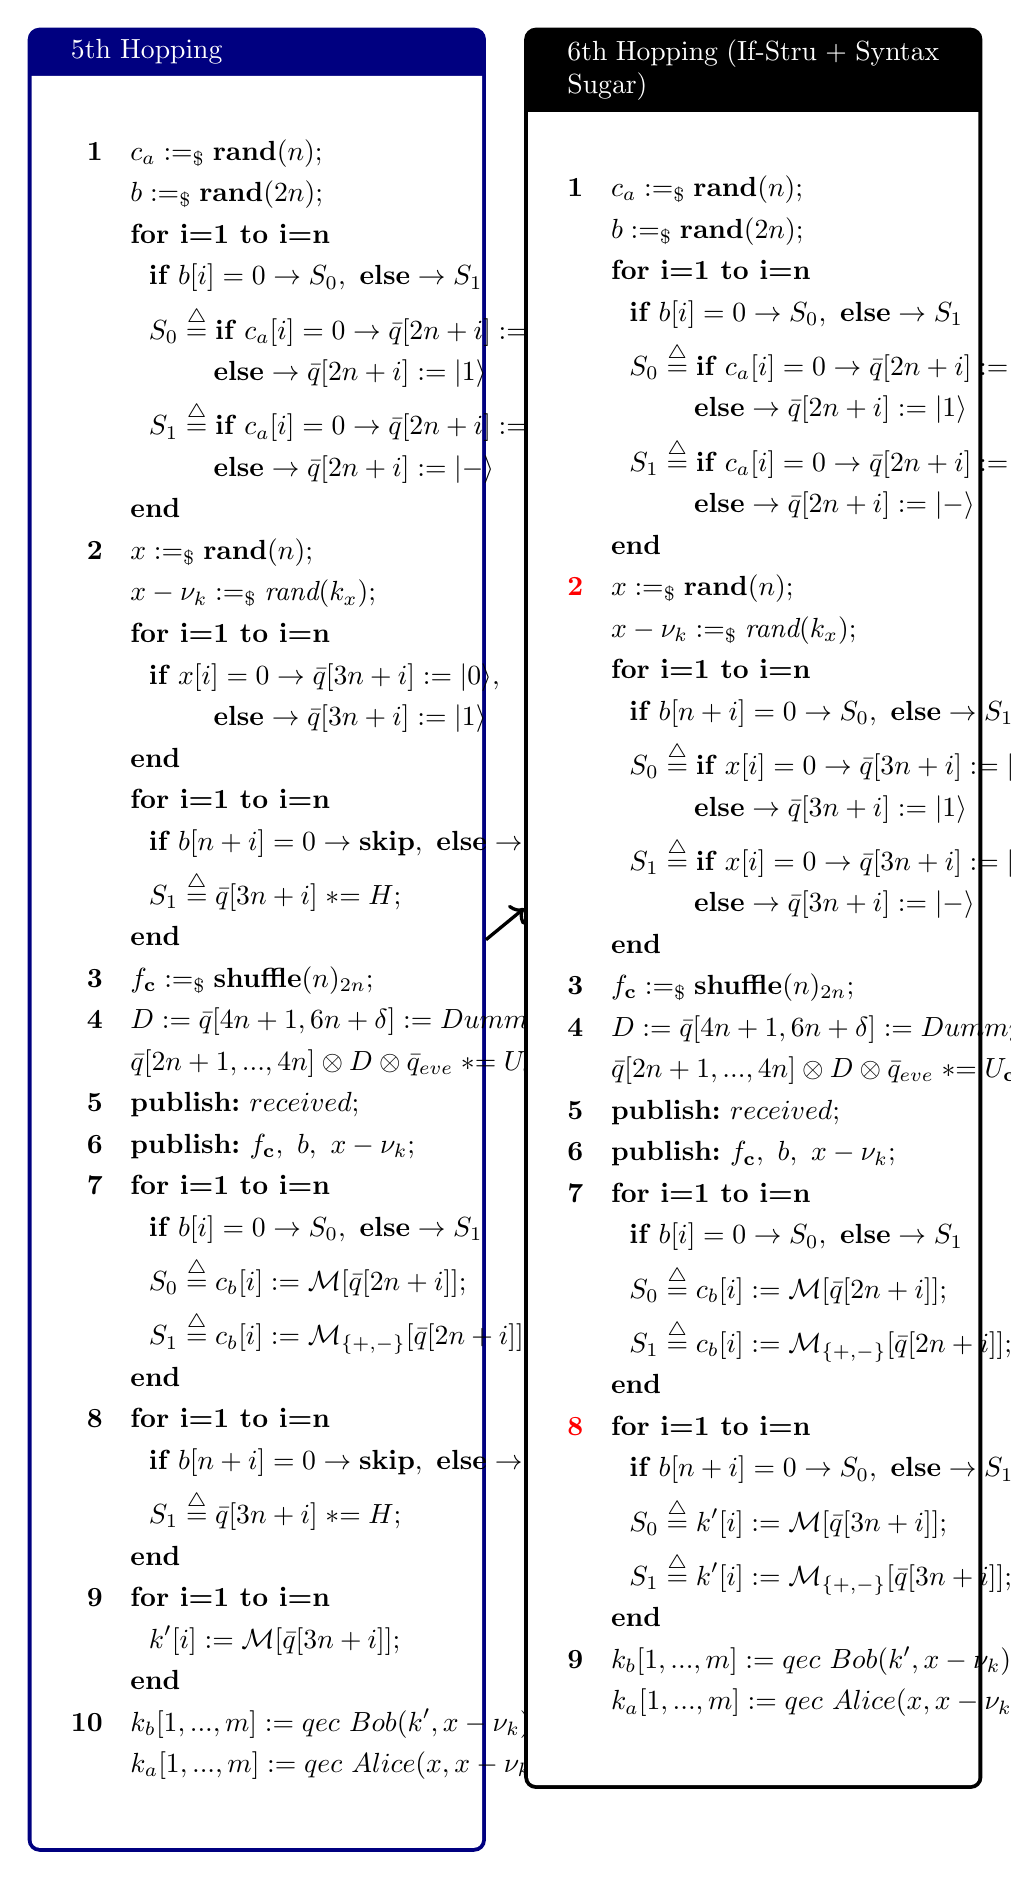
\begin{tikzpicture}[remember picture]

% Left box
\node[anchor=north west,inner sep=0pt,outer sep=0pt] (leftbox) at (0,0) {
\begin{minipage}[t]{0.48\textwidth}
\begin{tcolorbox}[colframe=blue!50!black, colback=white, title=5th Hopping, width=\textwidth]
\begin{align*}
    \textbf{{1}} \quad 
    & c_a :=_\$ \textbf{rand}(n); \\ 
    & b :=_\$ \textbf{rand}(2n); \\
    \quad 
    &\textbf{for~i=1~to~i=n}\\
    &~~ \textbf{if }  b[i] = 0 \rightarrow S_{0},~\textbf{else}\rightarrow S_{1}\\
    &~~ S_{0}\stackrel{\triangle}{=}\textbf{if }  c_a[i] = 0 \rightarrow \bar{q}[2n+i] := |0\rangle,\\ &~~~~~~~~~\textbf{else}   \rightarrow \bar{q}[2n+i] := |1\rangle\\
    &~~ S_{1}\stackrel{\triangle}{=}\textbf{if }  c_a[i] = 0 \rightarrow \bar{q}[2n+i] := |+\rangle,\\ &~~~~~~~~~\textbf{else}   \rightarrow \bar{q}[2n+i] := |-\rangle\\
    &\textbf{end}\\
    \textbf{{2}}\quad 
    & x :=_\$ \textbf{rand}(n); \\
    & x-\nu_k :=_\$ \textit{rand}(k_x);\\
    &\textbf{for~i=1~to~i=n}\\
    &~~ \textbf{if }  x[i] = 0 \rightarrow \bar{q}[3n+i] := |0\rangle,\\ &~~~~~~~~~\textbf{else}   \rightarrow \bar{q}[3n+i] := |1\rangle\\
    &\textbf{end}\\
    &\textbf{for~i=1~to~i=n}\\
    &~~ \textbf{if }  b[n+i] = 0 \rightarrow \textbf{skip},~\textbf{else}\rightarrow S_{1} ,\\
    &~~ S_{1}\stackrel{\triangle}{=}\bar{q}[3n+i] \asteq H ;\\
    &\textbf{end}\\
    \textbf{{3}} \quad & f_{\textbf{c}}:=_\$\textbf{shuffle}(n)_{2n}; \\
    \textbf{{4}} \quad & {D}:= \bar{q}[4n+1,6n+\delta]:=Dummy;\\     &\bar{q}[2n+1,...,4n]\otimes {D} \otimes \bar{q}_{eve} \asteq U_{\textbf{c}}(f_{\textbf{c}}); \\
    \textbf{{5}} \quad & \textbf{publish:}~ received;\\
    \textbf{{6}} \quad & \textbf{publish:}~ f_{\textbf{c}},~b,~x-\nu_k;\\
    \textbf{{7}} 
    \quad 
    &\textbf{for~i=1~to~i=n}\\
    &~~ \textbf{if }  b[i] = 0 \rightarrow S_{0},~\textbf{else}\rightarrow S_{1}\\
    &~~ S_{0}\stackrel{\triangle}{=}c_b[i]:= \mathcal{M} [\bar{q}[2n+i]];\\
    &~~ S_{1}\stackrel{\triangle}{=}c_b[i]:= \mathcal{M}_{\{+,-\}} [\bar{q}[2n+i]];\\
    &\textbf{end}\\
    \textbf{{8}}\quad 
    &\textbf{for~i=1~to~i=n}\\
    &~~ \textbf{if }  b[n+i] = 0 \rightarrow \textbf{skip},~\textbf{else}\rightarrow S_{1} ,\\
    &~~ S_{1}\stackrel{\triangle}{=}\bar{q}[3n+i] \asteq H ;\\
    &\textbf{end}\\
    \textbf{{9}} \quad 
    &\textbf{for~i=1~to~i=n}\\
    &~~ k'[i]:= \mathcal{M} [\bar{q}[3n+i]];\\
    &\textbf{end}\\
    {\textbf{10}} \quad & k_b[1,...,m]:=qec~Bob(k',x-\nu_k)\\
    &k_a[1,...,m]:=qec~Alice(x,x-\nu_k)\\
\end{align*}
\end{tcolorbox}
\end{minipage}
};

% Right box
\node[anchor=north west,inner sep=0pt,outer sep=0pt] (rightbox) at (0.52\textwidth,0) {
\begin{minipage}[t]{0.48\textwidth}
\begin{tcolorbox}[colframe=black!50!black, colback=white, title=6th Hopping (If-Stru + Syntax Sugar), width=\textwidth]
\begin{align*}
    \textbf{{1}} \quad 
    & c_a :=_\$ \textbf{rand}(n); \\ 
    & b :=_\$ \textbf{rand}(2n); \\
    \quad 
    &\textbf{for~i=1~to~i=n}\\
    &~~ \textbf{if }  b[i] = 0 \rightarrow S_{0},~\textbf{else}\rightarrow S_{1}\\
    &~~ S_{0}\stackrel{\triangle}{=}\textbf{if }  c_a[i] = 0 \rightarrow \bar{q}[2n+i] := |0\rangle,\\ &~~~~~~~~~\textbf{else}   \rightarrow \bar{q}[2n+i] := |1\rangle\\
    &~~ S_{1}\stackrel{\triangle}{=}\textbf{if }  c_a[i] = 0 \rightarrow \bar{q}[2n+i] := |+\rangle,\\ &~~~~~~~~~\textbf{else}   \rightarrow \bar{q}[2n+i] := |-\rangle\\
    &\textbf{end}\\
    \textbf{\textcolor{red}{2}}\quad 
    & x :=_\$ \textbf{rand}(n); \\
    & x-\nu_k :=_\$ \textit{rand}(k_x);\\
    &\textbf{for~i=1~to~i=n}\\
    &~~ \textbf{if }  b[n+i] = 0 \rightarrow S_{0},~\textbf{else}\rightarrow S_{1}\\
    &~~ S_{0}\stackrel{\triangle}{=}\textbf{if }  x[i] = 0 \rightarrow \bar{q}[3n+i] := |0\rangle,\\ &~~~~~~~~~\textbf{else}   \rightarrow \bar{q}[3n+i] := |1\rangle\\
    &~~ S_{1}\stackrel{\triangle}{=}\textbf{if }  x[i] = 0 \rightarrow \bar{q}[3n+i] := |+\rangle,\\ &~~~~~~~~~\textbf{else}   \rightarrow \bar{q}[3n+i] := |-\rangle\\
    &\textbf{end}\\
    \textbf{{3}} \quad & f_{\textbf{c}}:=_\$\textbf{shuffle}(n)_{2n}; \\
    \textbf{{4}} \quad & {D}:= \bar{q}[4n+1,6n+\delta]:=Dummy;\\     &\bar{q}[2n+1,...,4n]\otimes {D} \otimes \bar{q}_{eve} \asteq U_{\textbf{c}}(f_{\textbf{c}}); \\
    \textbf{{5}} \quad & \textbf{publish:}~ received;\\
    \textbf{{6}} \quad & \textbf{publish:}~ f_{\textbf{c}},~b,~x-\nu_k;\\
    \textbf{{7}} 
    \quad 
    &\textbf{for~i=1~to~i=n}\\
    &~~ \textbf{if }  b[i] = 0 \rightarrow S_{0},~\textbf{else}\rightarrow S_{1}\\
    &~~ S_{0}\stackrel{\triangle}{=}c_b[i]:= \mathcal{M} [\bar{q}[2n+i]];\\
    &~~ S_{1}\stackrel{\triangle}{=}c_b[i]:= \mathcal{M}_{\{+,-\}} [\bar{q}[2n+i]];\\
    &\textbf{end}\\
    \textbf{\textcolor{red}{8}}\quad 
    &\textbf{for~i=1~to~i=n}\\
    &~~ \textbf{if }  b[n+i] = 0 \rightarrow S_{0},~\textbf{else}\rightarrow S_{1}\\
    &~~ S_{0}\stackrel{\triangle}{=}k'[i]:= \mathcal{M} [\bar{q}[3n+i]];\\
    &~~ S_{1}\stackrel{\triangle}{=}k'[i]:= \mathcal{M}_{\{+,-\}} [\bar{q}[3n+i]];\\
    &\textbf{end}\\
    \textbf{{9}} \quad 
    &k_b[1,...,m]:=qec~Bob(k',x-\nu_k)\\
    &k_a[1,...,m]:=qec~Alice(x,x-\nu_k)\\
\end{align*}
\end{tcolorbox}
\end{minipage}
};

% Draw arrow between boxes
\draw[->, very thick] (leftbox.east) -- node[above]{} (rightbox.west);

\end{tikzpicture}
\newpage

\noindent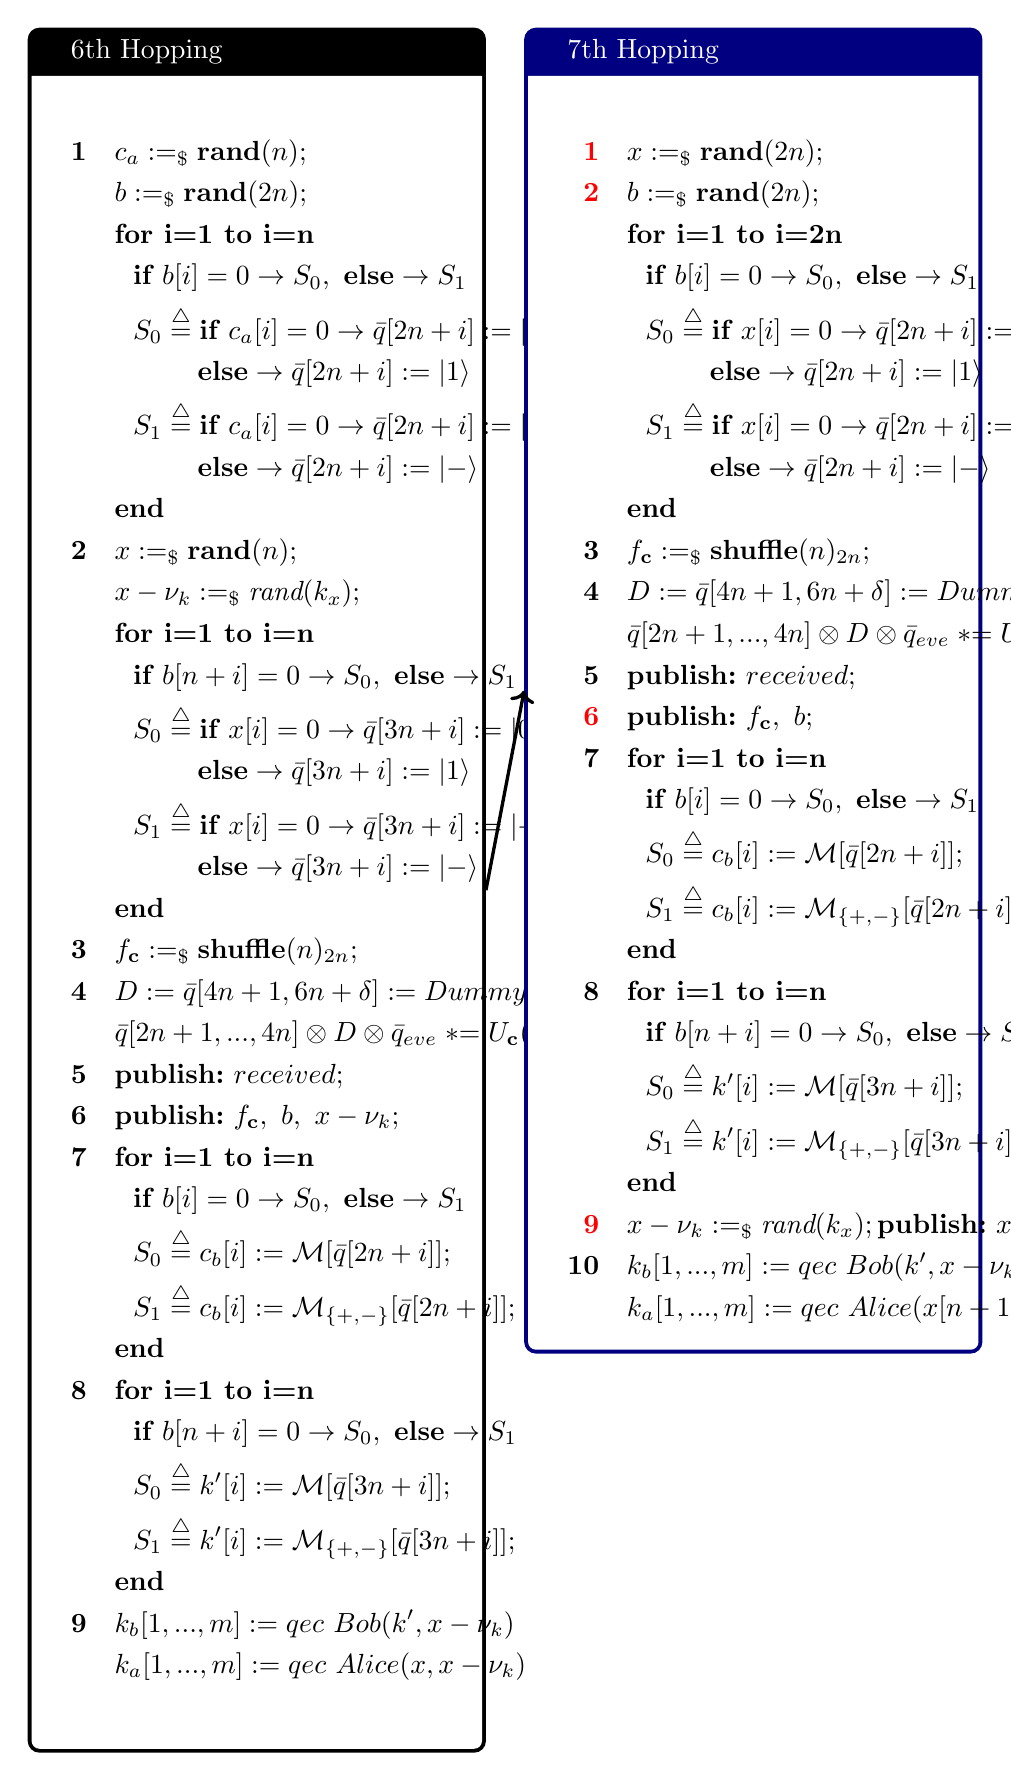
\begin{tikzpicture}[remember picture]

% Left box
\node[anchor=north west,inner sep=0pt,outer sep=0pt] (leftbox) at (0,0) {
\begin{minipage}[t]{0.48\textwidth}
\begin{tcolorbox}[colframe=black!50!black, colback=white, title=6th Hopping, width=\textwidth]
\begin{align*}
    \textbf{{1}} \quad 
    & c_a :=_\$ \textbf{rand}(n); \\ 
    & b :=_\$ \textbf{rand}(2n); \\
    \quad 
    &\textbf{for~i=1~to~i=n}\\
    &~~ \textbf{if }  b[i] = 0 \rightarrow S_{0},~\textbf{else}\rightarrow S_{1}\\
    &~~ S_{0}\stackrel{\triangle}{=}\textbf{if }  c_a[i] = 0 \rightarrow \bar{q}[2n+i] := |0\rangle,\\ &~~~~~~~~~\textbf{else}   \rightarrow \bar{q}[2n+i] := |1\rangle\\
    &~~ S_{1}\stackrel{\triangle}{=}\textbf{if }  c_a[i] = 0 \rightarrow \bar{q}[2n+i] := |+\rangle,\\ &~~~~~~~~~\textbf{else}   \rightarrow \bar{q}[2n+i] := |-\rangle\\
    &\textbf{end}\\
    \textbf{{2}}\quad 
    & x :=_\$ \textbf{rand}(n); \\
    & x-\nu_k :=_\$ \textit{rand}(k_x);\\
    &\textbf{for~i=1~to~i=n}\\
    &~~ \textbf{if }  b[n+i] = 0 \rightarrow S_{0},~\textbf{else}\rightarrow S_{1}\\
    &~~ S_{0}\stackrel{\triangle}{=}\textbf{if }  x[i] = 0 \rightarrow \bar{q}[3n+i] := |0\rangle,\\ &~~~~~~~~~\textbf{else}   \rightarrow \bar{q}[3n+i] := |1\rangle\\
    &~~ S_{1}\stackrel{\triangle}{=}\textbf{if }  x[i] = 0 \rightarrow \bar{q}[3n+i] := |+\rangle,\\ &~~~~~~~~~\textbf{else}   \rightarrow \bar{q}[3n+i] := |-\rangle\\
    &\textbf{end}\\
    \textbf{{3}} \quad & f_{\textbf{c}}:=_\$\textbf{shuffle}(n)_{2n}; \\
    \textbf{{4}} \quad & {D}:= \bar{q}[4n+1,6n+\delta]:=Dummy;\\     &\bar{q}[2n+1,...,4n]\otimes {D} \otimes \bar{q}_{eve} \asteq U_{\textbf{c}}(f_{\textbf{c}}); \\
    \textbf{{5}} \quad & \textbf{publish:}~ received;\\
    \textbf{{6}} \quad & \textbf{publish:}~ f_{\textbf{c}},~b,~x-\nu_k;\\
    \textbf{{7}} 
    \quad 
    &\textbf{for~i=1~to~i=n}\\
    &~~ \textbf{if }  b[i] = 0 \rightarrow S_{0},~\textbf{else}\rightarrow S_{1}\\
    &~~ S_{0}\stackrel{\triangle}{=}c_b[i]:= \mathcal{M} [\bar{q}[2n+i]];\\
    &~~ S_{1}\stackrel{\triangle}{=}c_b[i]:= \mathcal{M}_{\{+,-\}} [\bar{q}[2n+i]];\\
    &\textbf{end}\\
    \textbf{{8}}\quad 
    &\textbf{for~i=1~to~i=n}\\
    &~~ \textbf{if }  b[n+i] = 0 \rightarrow S_{0},~\textbf{else}\rightarrow S_{1}\\
    &~~ S_{0}\stackrel{\triangle}{=}k'[i]:= \mathcal{M} [\bar{q}[3n+i]];\\
    &~~ S_{1}\stackrel{\triangle}{=}k'[i]:= \mathcal{M}_{\{+,-\}} [\bar{q}[3n+i]];\\
    &\textbf{end}\\
    \textbf{{9}} \quad 
    &k_b[1,...,m]:=qec~Bob(k',x-\nu_k)\\
    &k_a[1,...,m]:=qec~Alice(x,x-\nu_k)\\
\end{align*}
\end{tcolorbox}
\end{minipage}
};


% Right box
\node[anchor=north west,inner sep=0pt,outer sep=0pt] (rightbox) at (0.52\textwidth,0) {
\begin{minipage}[t]{0.48\textwidth}
\begin{tcolorbox}[colframe=blue!50!black, colback=white, title=7th Hopping, width=\textwidth]
\begin{align*}
    \textbf{\textcolor{red}{1}} \quad 
    & x :=_\$ \textbf{rand}(2n); \\ 
    \textbf{\textcolor{red}{2}}\quad 
    & b :=_\$ \textbf{rand}(2n); \\
    &\textbf{for~i=1~to~i=2n}\\
    &~~ \textbf{if }  b[i] = 0 \rightarrow S_{0},~\textbf{else}\rightarrow S_{1}\\
    &~~ S_{0}\stackrel{\triangle}{=}\textbf{if }  x[i] = 0 \rightarrow \bar{q}[2n+i] := |0\rangle,\\ &~~~~~~~~~\textbf{else}   \rightarrow \bar{q}[2n+i] := |1\rangle\\
    &~~ S_{1}\stackrel{\triangle}{=}\textbf{if }  x[i] = 0 \rightarrow \bar{q}[2n+i] := |+\rangle,\\ &~~~~~~~~~\textbf{else}   \rightarrow \bar{q}[2n+i] := |-\rangle\\
    &\textbf{end}\\
    \textbf{{3}} \quad & f_{\textbf{c}}:=_\$\textbf{shuffle}(n)_{2n}; \\
    \textbf{{4}} \quad & {D}:= \bar{q}[4n+1,6n+\delta]:=Dummy;\\     &\bar{q}[2n+1,...,4n]\otimes {D} \otimes \bar{q}_{eve} \asteq U_{\textbf{c}}(f_{\textbf{c}}); \\
    \textbf{{5}} \quad & \textbf{publish:}~ received;\\
    \textbf{\textcolor{red}{6}} \quad & \textbf{publish:}~ f_{\textbf{c}},~b;\\
    \textbf{{7}} 
    \quad 
    &\textbf{for~i=1~to~i=n}\\
    &~~ \textbf{if }  b[i] = 0 \rightarrow S_{0},~\textbf{else}\rightarrow S_{1}\\
    &~~ S_{0}\stackrel{\triangle}{=}c_b[i]:= \mathcal{M} [\bar{q}[2n+i]];\\
    &~~ S_{1}\stackrel{\triangle}{=}c_b[i]:= \mathcal{M}_{\{+,-\}} [\bar{q}[2n+i]];\\
    &\textbf{end}\\
    \textbf{{8}}\quad 
    &\textbf{for~i=1~to~i=n}\\
    &~~ \textbf{if }  b[n+i] = 0 \rightarrow S_{0},~\textbf{else}\rightarrow S_{1}\\
    &~~ S_{0}\stackrel{\triangle}{=}k'[i]:= \mathcal{M} [\bar{q}[3n+i]];\\
    &~~ S_{1}\stackrel{\triangle}{=}k'[i]:= \mathcal{M}_{\{+,-\}} [\bar{q}[3n+i]];\\
    &\textbf{end}\\
    \textbf{\textcolor{red}{9}} \quad & x-\nu_k :=_\$ \textit{rand}(k_x); \textbf{publish:}~ x-\nu_k;\\
    \textbf{{10}} \quad 
    &k_b[1,...,m]:=qec~Bob(k',x-\nu_k)\\
    &k_a[1,...,m]:=qec~Alice(x[n+1,...,2n],x-\nu_k)
\end{align*}
\end{tcolorbox}
\end{minipage}
};

% Draw arrow between boxes
\draw[->, very thick] (leftbox.east) -- node[above]{} (rightbox.west);

\end{tikzpicture}
\newpage

\noindent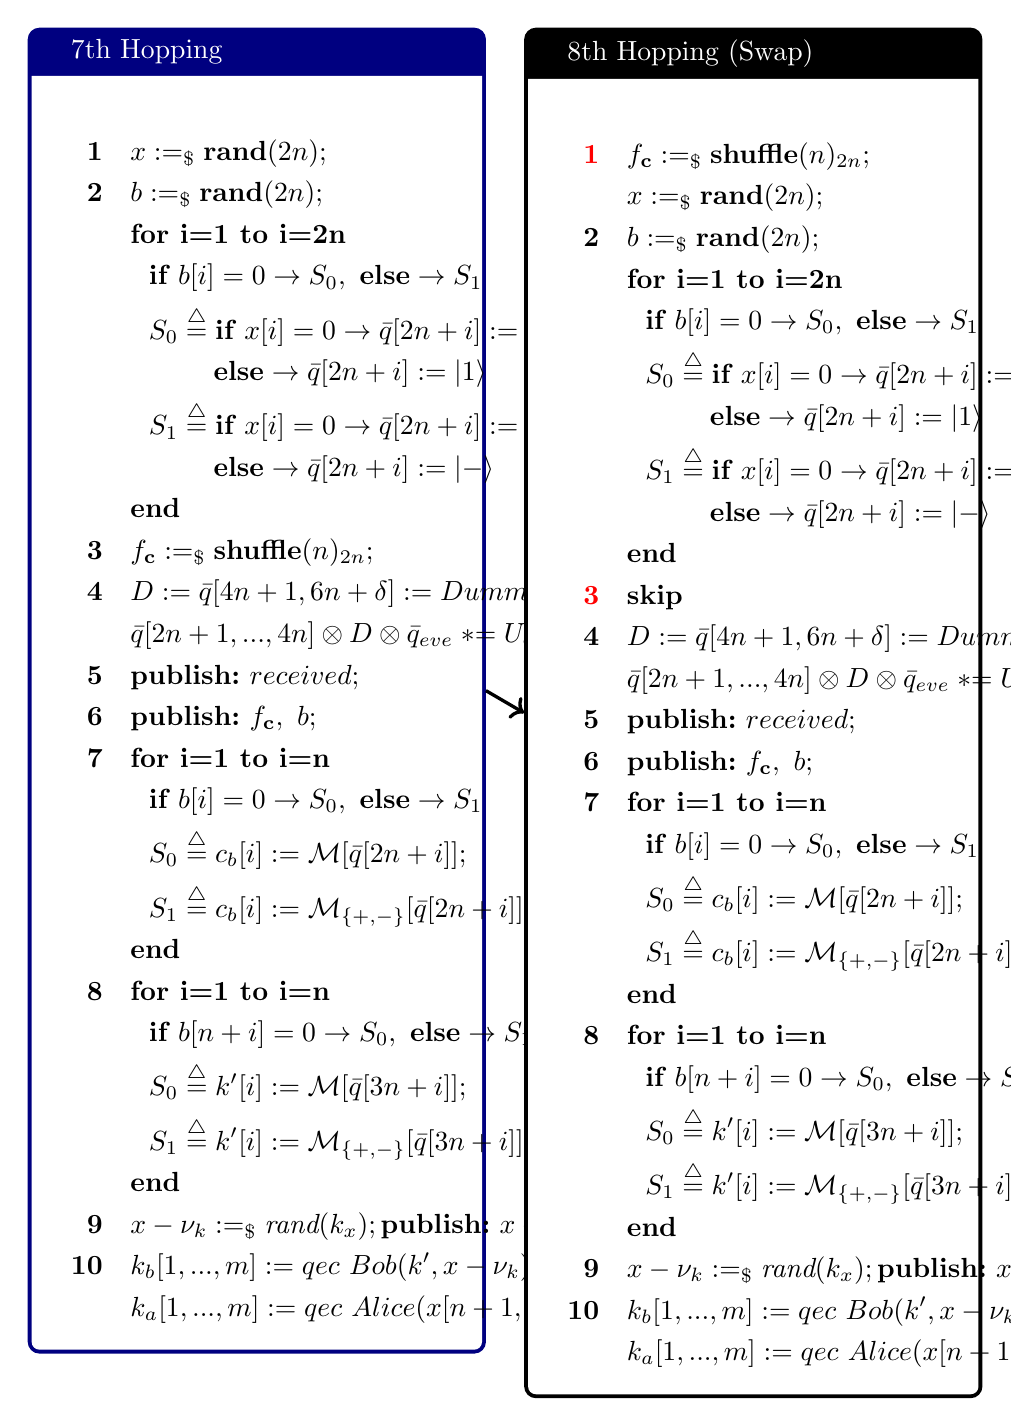
\begin{tikzpicture}[remember picture]

% Left box
\node[anchor=north west,inner sep=0pt,outer sep=0pt] (leftbox) at (0,0) {
\begin{minipage}[t]{0.48\textwidth}
\begin{tcolorbox}[colframe=blue!50!black, colback=white, title=7th Hopping, width=\textwidth]
\begin{align*}
    \textbf{{1}} \quad 
    & x :=_\$ \textbf{rand}(2n); \\ 
    \textbf{{2}}\quad 
    & b :=_\$ \textbf{rand}(2n); \\
    &\textbf{for~i=1~to~i=2n}\\
    &~~ \textbf{if }  b[i] = 0 \rightarrow S_{0},~\textbf{else}\rightarrow S_{1}\\
    &~~ S_{0}\stackrel{\triangle}{=}\textbf{if }  x[i] = 0 \rightarrow \bar{q}[2n+i] := |0\rangle,\\ &~~~~~~~~~\textbf{else}   \rightarrow \bar{q}[2n+i] := |1\rangle\\
    &~~ S_{1}\stackrel{\triangle}{=}\textbf{if }  x[i] = 0 \rightarrow \bar{q}[2n+i] := |+\rangle,\\ &~~~~~~~~~\textbf{else}   \rightarrow \bar{q}[2n+i] := |-\rangle\\
    &\textbf{end}\\
    \textbf{{3}} \quad & f_{\textbf{c}}:=_\$\textbf{shuffle}(n)_{2n}; \\
    \textbf{{4}} \quad & {D}:= \bar{q}[4n+1,6n+\delta]:=Dummy;\\     &\bar{q}[2n+1,...,4n]\otimes {D} \otimes \bar{q}_{eve} \asteq U_{\textbf{c}}(f_{\textbf{c}}); \\
    \textbf{{5}} \quad & \textbf{publish:}~ received;\\
    \textbf{{6}} \quad & \textbf{publish:}~ f_{\textbf{c}},~b;\\
    \textbf{{7}} 
    \quad 
    &\textbf{for~i=1~to~i=n}\\
    &~~ \textbf{if }  b[i] = 0 \rightarrow S_{0},~\textbf{else}\rightarrow S_{1}\\
    &~~ S_{0}\stackrel{\triangle}{=}c_b[i]:= \mathcal{M} [\bar{q}[2n+i]];\\
    &~~ S_{1}\stackrel{\triangle}{=}c_b[i]:= \mathcal{M}_{\{+,-\}} [\bar{q}[2n+i]];\\
    &\textbf{end}\\
    \textbf{{8}}\quad 
    &\textbf{for~i=1~to~i=n}\\
    &~~ \textbf{if }  b[n+i] = 0 \rightarrow S_{0},~\textbf{else}\rightarrow S_{1}\\
    &~~ S_{0}\stackrel{\triangle}{=}k'[i]:= \mathcal{M} [\bar{q}[3n+i]];\\
    &~~ S_{1}\stackrel{\triangle}{=}k'[i]:= \mathcal{M}_{\{+,-\}} [\bar{q}[3n+i]];\\
    &\textbf{end}\\
    \textbf{{9}} \quad & x-\nu_k :=_\$ \textit{rand}(k_x); \textbf{publish:}~ x-\nu_k;\\
    \textbf{{10}} \quad 
    &k_b[1,...,m]:=qec~Bob(k',x-\nu_k)\\
    &k_a[1,...,m]:=qec~Alice(x[n+1,...,2n],x-\nu_k)
\end{align*}
\end{tcolorbox}
\end{minipage}
};

% Right box
\node[anchor=north west,inner sep=0pt,outer sep=0pt] (rightbox) at (0.52\textwidth,0) {
\begin{minipage}[t]{0.48\textwidth}
\begin{tcolorbox}[colframe=black!50!black, colback=white, title=8th Hopping (Swap), width=\textwidth]
\begin{align*}
    \textbf{\textcolor{red}{1}} \quad 
    &f_{\textbf{c}}:=_\$\textbf{shuffle}(n)_{2n}; \\
    &x :=_\$ \textbf{rand}(2n); \\ 
    \textbf{{2}}\quad 
    & b :=_\$ \textbf{rand}(2n); \\
    &\textbf{for~i=1~to~i=2n}\\
    &~~ \textbf{if }  b[i] = 0 \rightarrow S_{0},~\textbf{else}\rightarrow S_{1}\\
    &~~ S_{0}\stackrel{\triangle}{=}\textbf{if }  x[i] = 0 \rightarrow \bar{q}[2n+i] := |0\rangle,\\ &~~~~~~~~~\textbf{else}   \rightarrow \bar{q}[2n+i] := |1\rangle\\
    &~~ S_{1}\stackrel{\triangle}{=}\textbf{if }  x[i] = 0 \rightarrow \bar{q}[2n+i] := |+\rangle,\\ &~~~~~~~~~\textbf{else}   \rightarrow \bar{q}[2n+i] := |-\rangle\\
    &\textbf{end}\\
    \textbf{\textcolor{red}{3}} \quad & \textbf{skip}\\
    \textbf{{4}} \quad & {D}:= \bar{q}[4n+1,6n+\delta]:=Dummy;\\     &\bar{q}[2n+1,...,4n]\otimes {D} \otimes \bar{q}_{eve} \asteq U_{\textbf{c}}(f_{\textbf{c}}); \\
    \textbf{{5}} \quad & \textbf{publish:}~ received;\\
    \textbf{{6}} \quad & \textbf{publish:}~ f_{\textbf{c}},~b;\\
    \textbf{{7}} 
    \quad 
    &\textbf{for~i=1~to~i=n}\\
    &~~ \textbf{if }  b[i] = 0 \rightarrow S_{0},~\textbf{else}\rightarrow S_{1}\\
    &~~ S_{0}\stackrel{\triangle}{=}c_b[i]:= \mathcal{M} [\bar{q}[2n+i]];\\
    &~~ S_{1}\stackrel{\triangle}{=}c_b[i]:= \mathcal{M}_{\{+,-\}} [\bar{q}[2n+i]];\\
    &\textbf{end}\\
    \textbf{{8}}\quad 
    &\textbf{for~i=1~to~i=n}\\
    &~~ \textbf{if }  b[n+i] = 0 \rightarrow S_{0},~\textbf{else}\rightarrow S_{1}\\
    &~~ S_{0}\stackrel{\triangle}{=}k'[i]:= \mathcal{M} [\bar{q}[3n+i]];\\
    &~~ S_{1}\stackrel{\triangle}{=}k'[i]:= \mathcal{M}_{\{+,-\}} [\bar{q}[3n+i]];\\
    &\textbf{end}\\
    \textbf{{9}} \quad & x-\nu_k :=_\$ \textit{rand}(k_x); \textbf{publish:}~ x-\nu_k;\\
    \textbf{{10}} \quad 
    &k_b[1,...,m]:=qec~Bob(k',x-\nu_k)\\
    &k_a[1,...,m]:=qec~Alice(x[n+1,...,2n],x-\nu_k)
\end{align*}
\end{tcolorbox}
\end{minipage}
};

% Draw arrow between boxes
\draw[->, very thick] (leftbox.east) -- node[above]{} (rightbox.west);

\end{tikzpicture}

\newpage


\noindent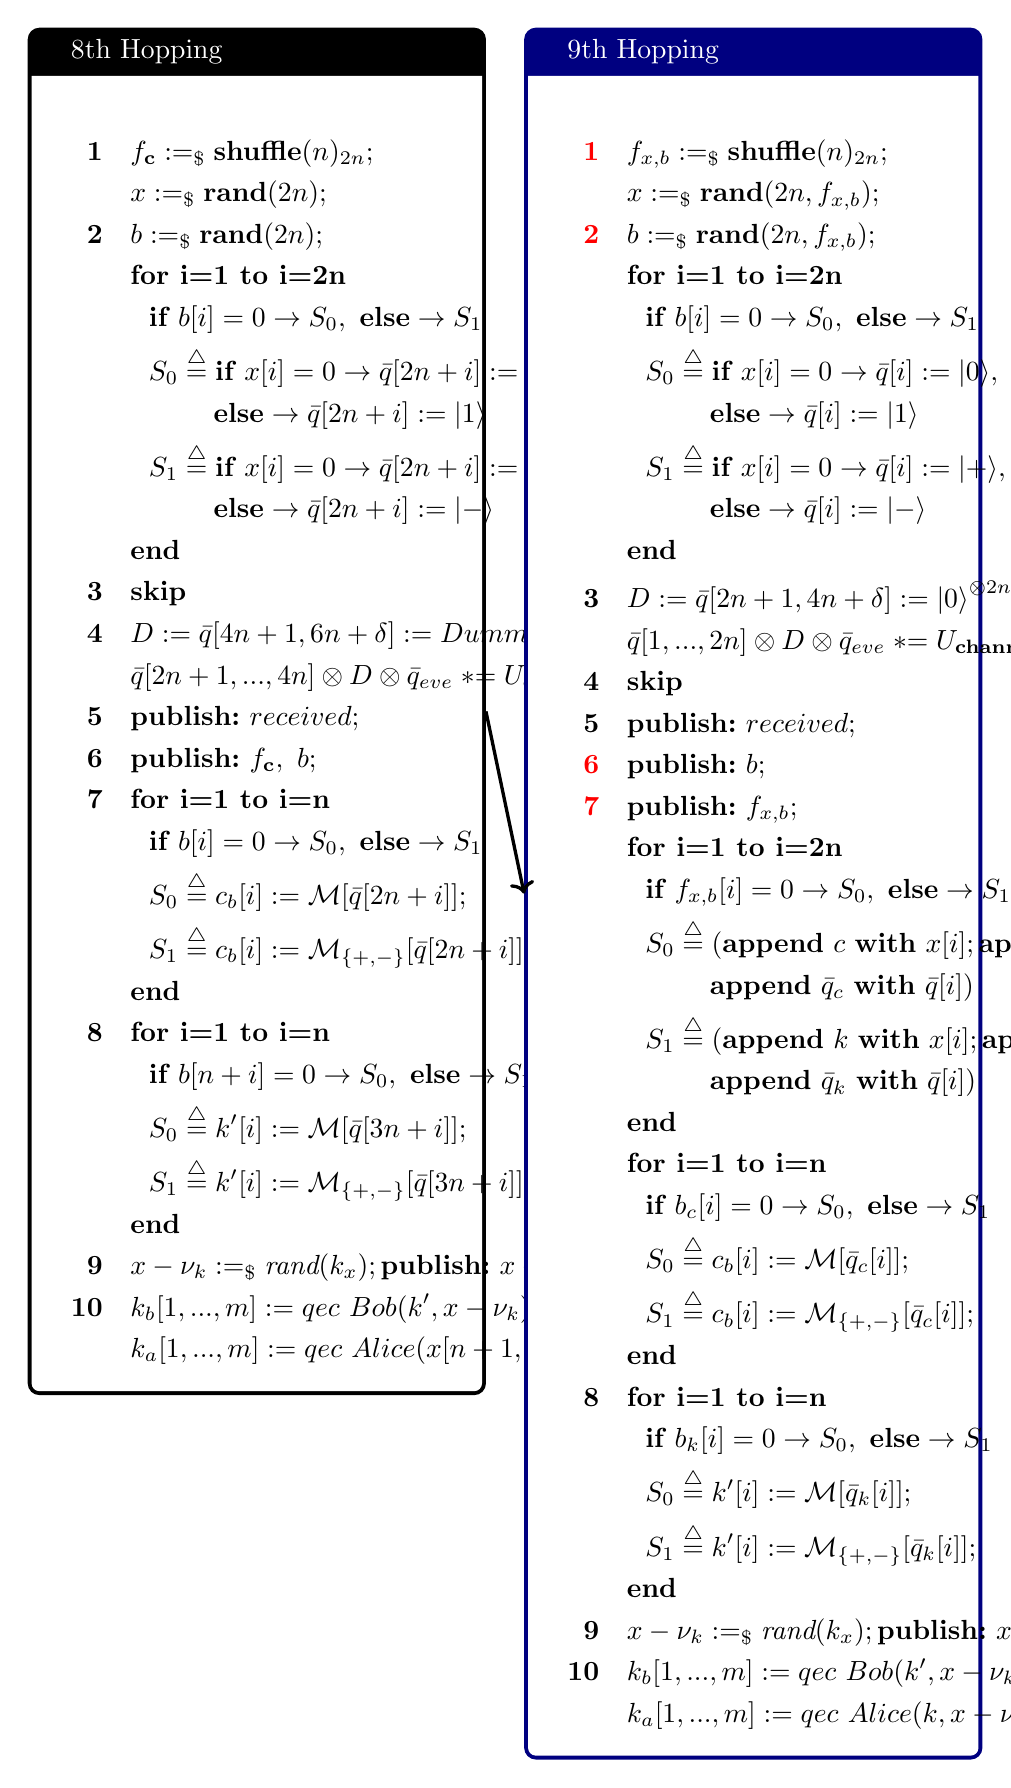
\begin{tikzpicture}[remember picture]

% Left box
\node[anchor=north west,inner sep=0pt,outer sep=0pt] (leftbox) at (0,0) {
\begin{minipage}[t]{0.48\textwidth}
\begin{tcolorbox}[colframe=black!50!black, colback=white, title=8th Hopping, width=\textwidth]
\begin{align*}
    \textbf{{1}} \quad 
    &f_{\textbf{c}}:=_\$\textbf{shuffle}(n)_{2n}; \\
    &x :=_\$ \textbf{rand}(2n); \\ 
    \textbf{{2}}\quad 
    & b :=_\$ \textbf{rand}(2n); \\
    &\textbf{for~i=1~to~i=2n}\\
    &~~ \textbf{if }  b[i] = 0 \rightarrow S_{0},~\textbf{else}\rightarrow S_{1}\\
    &~~ S_{0}\stackrel{\triangle}{=}\textbf{if }  x[i] = 0 \rightarrow \bar{q}[2n+i] := |0\rangle,\\ &~~~~~~~~~\textbf{else}   \rightarrow \bar{q}[2n+i] := |1\rangle\\
    &~~ S_{1}\stackrel{\triangle}{=}\textbf{if }  x[i] = 0 \rightarrow \bar{q}[2n+i] := |+\rangle,\\ &~~~~~~~~~\textbf{else}   \rightarrow \bar{q}[2n+i] := |-\rangle\\
    &\textbf{end}\\
    \textbf{{3}} \quad & \textbf{skip}\\
    \textbf{{4}} \quad & {D}:= \bar{q}[4n+1,6n+\delta]:=Dummy;\\     &\bar{q}[2n+1,...,4n]\otimes {D} \otimes \bar{q}_{eve} \asteq U_{\textbf{c}}(f_{\textbf{c}}); \\
    \textbf{{5}} \quad & \textbf{publish:}~ received;\\
    \textbf{{6}} \quad & \textbf{publish:}~ f_{\textbf{c}},~b;\\
    \textbf{{7}} 
    \quad 
    &\textbf{for~i=1~to~i=n}\\
    &~~ \textbf{if }  b[i] = 0 \rightarrow S_{0},~\textbf{else}\rightarrow S_{1}\\
    &~~ S_{0}\stackrel{\triangle}{=}c_b[i]:= \mathcal{M} [\bar{q}[2n+i]];\\
    &~~ S_{1}\stackrel{\triangle}{=}c_b[i]:= \mathcal{M}_{\{+,-\}} [\bar{q}[2n+i]];\\
    &\textbf{end}\\
    \textbf{{8}}\quad 
    &\textbf{for~i=1~to~i=n}\\
    &~~ \textbf{if }  b[n+i] = 0 \rightarrow S_{0},~\textbf{else}\rightarrow S_{1}\\
    &~~ S_{0}\stackrel{\triangle}{=}k'[i]:= \mathcal{M} [\bar{q}[3n+i]];\\
    &~~ S_{1}\stackrel{\triangle}{=}k'[i]:= \mathcal{M}_{\{+,-\}} [\bar{q}[3n+i]];\\
    &\textbf{end}\\
    \textbf{{9}} \quad & x-\nu_k :=_\$ \textit{rand}(k_x); \textbf{publish:}~ x-\nu_k;\\
    \textbf{{10}} \quad 
    &k_b[1,...,m]:=qec~Bob(k',x-\nu_k)\\
    &k_a[1,...,m]:=qec~Alice(x[n+1,...,2n],x-\nu_k)
\end{align*}
\end{tcolorbox}
\end{minipage}
};

% Right box
\node[anchor=north west,inner sep=0pt,outer sep=0pt] (rightbox) at (0.52\textwidth,0) {
\begin{minipage}[t]{0.48\textwidth}
\begin{tcolorbox}[colframe=blue!50!black, colback=white, title=9th Hopping, width=\textwidth]
\begin{align*}
    \textbf{\textcolor{red}{1}} \quad 
    & f_{x,b}:=_\$\textbf{shuffle}(n)_{2n}; \\
    &x :=_\$ \textbf{rand}(2n,f_{x,b}); \\ 
    \textbf{\textcolor{red}{2}}\quad 
    & b :=_\$ \textbf{rand}(2n,f_{x,b}); \\
    &\textbf{for~i=1~to~i=2n}\\
    &~~ \textbf{if }  b[i] = 0 \rightarrow S_{0},~\textbf{else}\rightarrow S_{1}\\
    &~~ S_{0}\stackrel{\triangle}{=}\textbf{if }  x[i] = 0 \rightarrow \bar{q}[i] := |0\rangle,\\ &~~~~~~~~~\textbf{else}   \rightarrow \bar{q}[i] := |1\rangle\\
    &~~ S_{1}\stackrel{\triangle}{=}\textbf{if }  x[i] = 0 \rightarrow \bar{q}[i] := |+\rangle,\\ &~~~~~~~~~\textbf{else}   \rightarrow \bar{q}[i] := |-\rangle\\
    &\textbf{end}\\
    \textbf{{3}} 
    \quad & {D}:= \bar{q}[2n+1,4n+\delta]:=\ket{0}^{\otimes 2n+\delta};\\     &\bar{q}[1,...,2n]\otimes {D} \otimes \bar{q}_{eve} \asteq U_{\textbf{channel}}; \\
    \textbf{{4}} \quad &\textbf{skip} \\ 
    \textbf{{5}} \quad & \textbf{publish:}~ received;\\
    \textbf{\textcolor{red}{6}} \quad & \textbf{publish:}~b;\\
    \textbf{\textcolor{red}{7}} 
    \quad & \textbf{publish:}~ f_{x,b};\\
    &\textbf{for~i=1~to~i=2n}\\
    &~~ \textbf{if }  f_{x,b}[i] = 0 \rightarrow S_{0},~\textbf{else}\rightarrow S_{1}\\
    &~~ S_{0}\stackrel{\triangle}{=}(\textbf{append}~c~\textbf{with}~x[i];\textbf{append}~b_c~\textbf{with}~b[i];\\
    &\qquad\quad\textbf{append}~\bar{q}_c~\textbf{with}~\bar{q}[i])\\
    &~~ S_{1}\stackrel{\triangle}{=}(\textbf{append}~k~\textbf{with}~x[i];\textbf{append}~b_k~\textbf{with}~b[i];\\
    &\qquad\quad\textbf{append}~\bar{q}_k~\textbf{with}~\bar{q}[i])\\
    &\textbf{end}\\
    &\textbf{for~i=1~to~i=n}\\
    &~~ \textbf{if }  b_c[i] = 0 \rightarrow S_{0},~\textbf{else}\rightarrow S_{1}\\
    &~~ S_{0}\stackrel{\triangle}{=}c_b[i]:= \mathcal{M} [\bar{q}_c[i]];\\
    &~~ S_{1}\stackrel{\triangle}{=}c_b[i]:= \mathcal{M}_{\{+,-\}} [\bar{q}_c[i]];\\
    &\textbf{end}\\
    \textbf{{8}}\quad 
    &\textbf{for~i=1~to~i=n}\\
    &~~ \textbf{if }  b_k[i] = 0 \rightarrow S_{0},~\textbf{else}\rightarrow S_{1}\\
    &~~ S_{0}\stackrel{\triangle}{=}k'[i]:= \mathcal{M} [\bar{q}_k[i]];\\
    &~~ S_{1}\stackrel{\triangle}{=}k'[i]:= \mathcal{M}_{\{+,-\}} [\bar{q}_k[i]];\\
    &\textbf{end}\\
    \textbf{{9}} \quad & x-\nu_k :=_\$ \textit{rand}(k_x); \textbf{publish:}~ x-\nu_k;\\
    \textbf{{10}} \quad 
    &k_b[1,...,m]:=qec~Bob(k',x-\nu_k)\\
    &k_a[1,...,m]:=qec~Alice(k,x-\nu_k)
\end{align*}
\end{tcolorbox}
\end{minipage}
};

% Draw arrow between boxes
\draw[->, very thick] (leftbox.east) -- node[above]{} (rightbox.west);

\end{tikzpicture}
\newpage

\noindent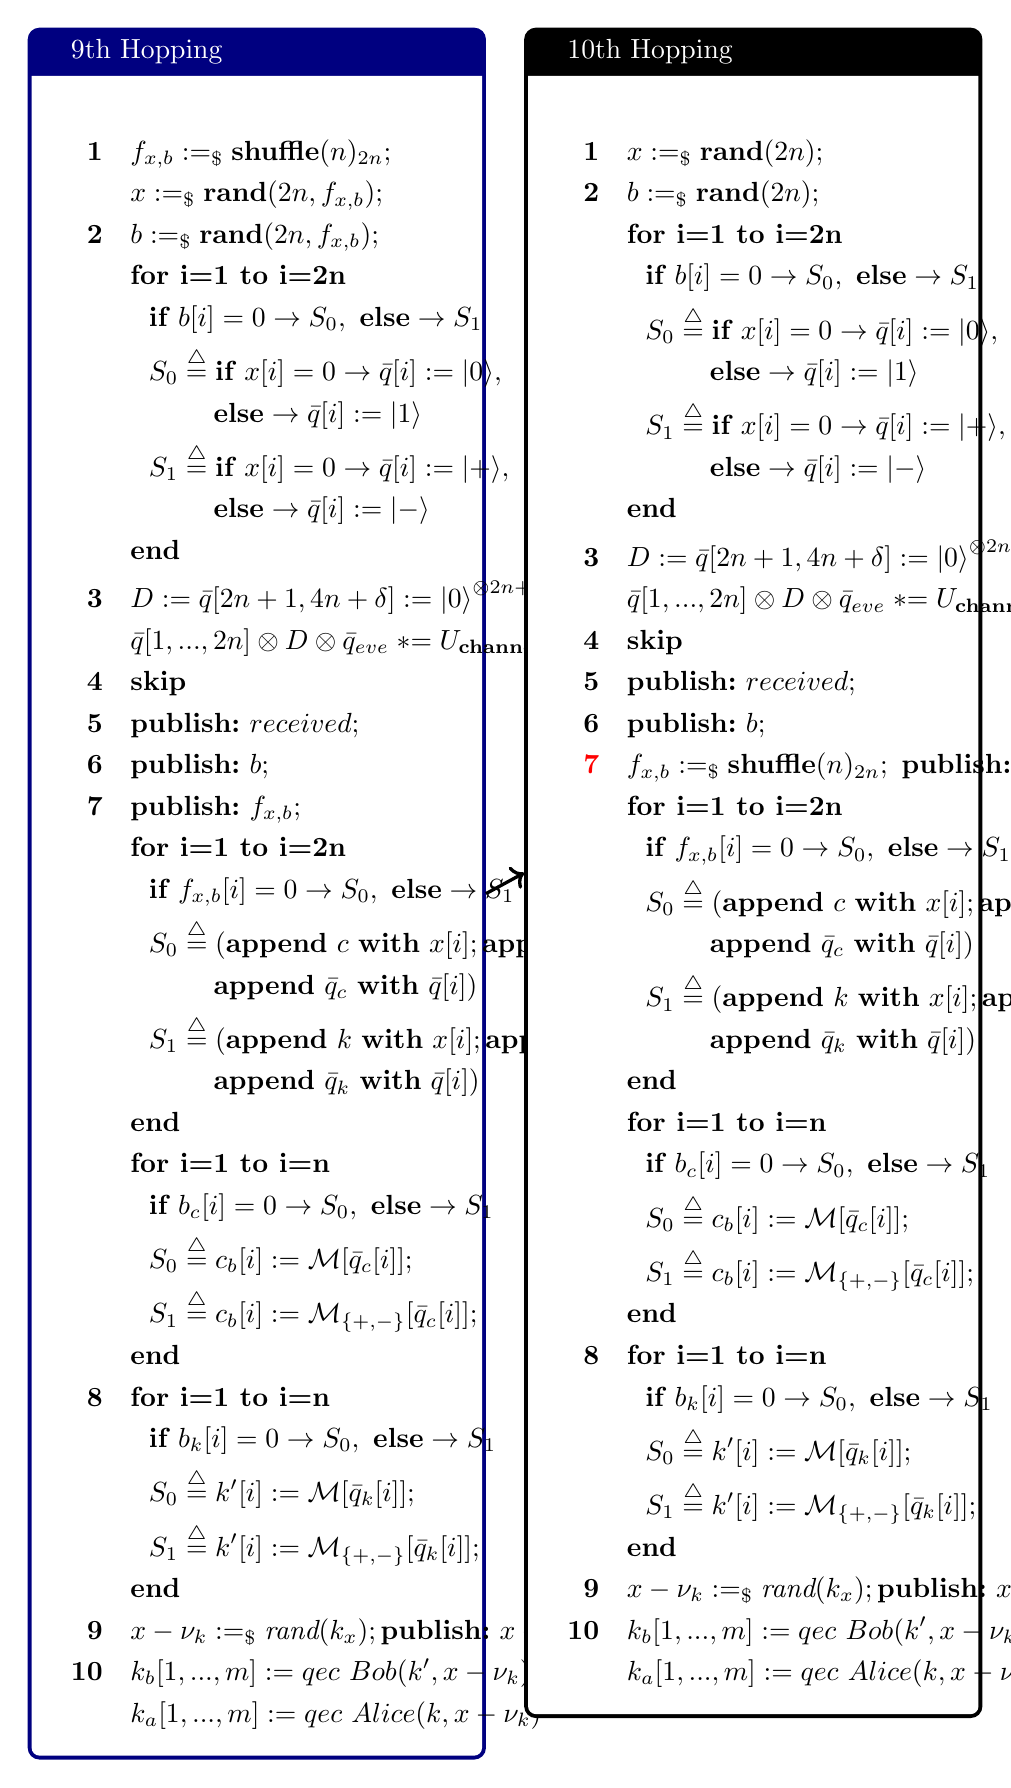
\begin{tikzpicture}[remember picture]

% Left box
\node[anchor=north west,inner sep=0pt,outer sep=0pt] (leftbox) at (0,0) {
\begin{minipage}[t]{0.48\textwidth}
\begin{tcolorbox}[colframe=blue!50!black, colback=white, title=9th Hopping, width=\textwidth]
\begin{align*}
    \textbf{{1}} \quad 
    & f_{x,b}:=_\$\textbf{shuffle}(n)_{2n}; \\
    &x :=_\$ \textbf{rand}(2n,f_{x,b}); \\ 
    \textbf{{2}}\quad 
    & b :=_\$ \textbf{rand}(2n,f_{x,b}); \\
    &\textbf{for~i=1~to~i=2n}\\
    &~~ \textbf{if }  b[i] = 0 \rightarrow S_{0},~\textbf{else}\rightarrow S_{1}\\
    &~~ S_{0}\stackrel{\triangle}{=}\textbf{if }  x[i] = 0 \rightarrow \bar{q}[i] := |0\rangle,\\ &~~~~~~~~~\textbf{else}   \rightarrow \bar{q}[i] := |1\rangle\\
    &~~ S_{1}\stackrel{\triangle}{=}\textbf{if }  x[i] = 0 \rightarrow \bar{q}[i] := |+\rangle,\\ &~~~~~~~~~\textbf{else}   \rightarrow \bar{q}[i] := |-\rangle\\
    &\textbf{end}\\
    \textbf{{3}} 
    \quad & {D}:= \bar{q}[2n+1,4n+\delta]:=\ket{0}^{\otimes 2n+\delta};\\     &\bar{q}[1,...,2n]\otimes {D} \otimes \bar{q}_{eve} \asteq U_{\textbf{channel}}; \\
    \textbf{{4}} \quad &\textbf{skip} \\ 
    \textbf{{5}} \quad & \textbf{publish:}~ received;\\
    \textbf{{6}} \quad & \textbf{publish:}~b;\\
    \textbf{{7}} 
    \quad & \textbf{publish:}~ f_{x,b};\\
    &\textbf{for~i=1~to~i=2n}\\
    &~~ \textbf{if }  f_{x,b}[i] = 0 \rightarrow S_{0},~\textbf{else}\rightarrow S_{1}\\
    &~~ S_{0}\stackrel{\triangle}{=}(\textbf{append}~c~\textbf{with}~x[i];\textbf{append}~b_c~\textbf{with}~b[i];\\
    &\qquad\quad\textbf{append}~\bar{q}_c~\textbf{with}~\bar{q}[i])\\
    &~~ S_{1}\stackrel{\triangle}{=}(\textbf{append}~k~\textbf{with}~x[i];\textbf{append}~b_k~\textbf{with}~b[i];\\
    &\qquad\quad\textbf{append}~\bar{q}_k~\textbf{with}~\bar{q}[i])\\
    &\textbf{end}\\
    &\textbf{for~i=1~to~i=n}\\
    &~~ \textbf{if }  b_c[i] = 0 \rightarrow S_{0},~\textbf{else}\rightarrow S_{1}\\
    &~~ S_{0}\stackrel{\triangle}{=}c_b[i]:= \mathcal{M} [\bar{q}_c[i]];\\
    &~~ S_{1}\stackrel{\triangle}{=}c_b[i]:= \mathcal{M}_{\{+,-\}} [\bar{q}_c[i]];\\
    &\textbf{end}\\
    \textbf{{8}}\quad 
    &\textbf{for~i=1~to~i=n}\\
    &~~ \textbf{if }  b_k[i] = 0 \rightarrow S_{0},~\textbf{else}\rightarrow S_{1}\\
    &~~ S_{0}\stackrel{\triangle}{=}k'[i]:= \mathcal{M} [\bar{q}_k[i]];\\
    &~~ S_{1}\stackrel{\triangle}{=}k'[i]:= \mathcal{M}_{\{+,-\}} [\bar{q}_k[i]];\\
    &\textbf{end}\\
    \textbf{{9}} \quad & x-\nu_k :=_\$ \textit{rand}(k_x); \textbf{publish:}~ x-\nu_k;\\
    \textbf{{10}} \quad 
    &k_b[1,...,m]:=qec~Bob(k',x-\nu_k)\\
    &k_a[1,...,m]:=qec~Alice(k,x-\nu_k)
\end{align*}
\end{tcolorbox}
\end{minipage}
};

% Right box
\node[anchor=north west,inner sep=0pt,outer sep=0pt] (rightbox) at (0.52\textwidth,0) {
\begin{minipage}[t]{0.48\textwidth}
\begin{tcolorbox}[colframe=black!50!black, colback=white, title=10th Hopping, width=\textwidth]
\begin{align*}
    \textbf{{1}} \quad 
    &x :=_\$ \textbf{rand}(2n); \\ 
    \textbf{{2}}\quad 
    & b :=_\$ \textbf{rand}(2n); \\
    &\textbf{for~i=1~to~i=2n}\\
    &~~ \textbf{if }  b[i] = 0 \rightarrow S_{0},~\textbf{else}\rightarrow S_{1}\\
    &~~ S_{0}\stackrel{\triangle}{=}\textbf{if }  x[i] = 0 \rightarrow \bar{q}[i] := |0\rangle,\\ &~~~~~~~~~\textbf{else}   \rightarrow \bar{q}[i] := |1\rangle\\
    &~~ S_{1}\stackrel{\triangle}{=}\textbf{if }  x[i] = 0 \rightarrow \bar{q}[i] := |+\rangle,\\ &~~~~~~~~~\textbf{else}   \rightarrow \bar{q}[i] := |-\rangle\\
    &\textbf{end}\\
    \textbf{{3}} 
    \quad & {D}:= \bar{q}[2n+1,4n+\delta]:=\ket{0}^{\otimes 2n+\delta};\\     &\bar{q}[1,...,2n]\otimes {D} \otimes \bar{q}_{eve} \asteq U_{\textbf{channel}}; \\
    \textbf{{4}} \quad &\textbf{skip} \\ 
    \textbf{{5}} \quad & \textbf{publish:}~ received;\\
    \textbf{{6}} \quad & \textbf{publish:}~b;\\
    \textbf{\textcolor{red}{7}} 
    \quad &f_{x,b}:=_\$\textbf{shuffle}(n)_{2n}; ~ \textbf{publish:}~ f_{x,b};\\
    &\textbf{for~i=1~to~i=2n}\\
    &~~ \textbf{if }  f_{x,b}[i] = 0 \rightarrow S_{0},~\textbf{else}\rightarrow S_{1}\\
    &~~ S_{0}\stackrel{\triangle}{=}(\textbf{append}~c~\textbf{with}~x[i];\textbf{append}~b_c~\textbf{with}~b[i];\\
    &\qquad\quad\textbf{append}~\bar{q}_c~\textbf{with}~\bar{q}[i])\\
    &~~ S_{1}\stackrel{\triangle}{=}(\textbf{append}~k~\textbf{with}~x[i];\textbf{append}~b_k~\textbf{with}~b[i];\\
    &\qquad\quad\textbf{append}~\bar{q}_k~\textbf{with}~\bar{q}[i])\\
    &\textbf{end}\\
    &\textbf{for~i=1~to~i=n}\\
    &~~ \textbf{if }  b_c[i] = 0 \rightarrow S_{0},~\textbf{else}\rightarrow S_{1}\\
    &~~ S_{0}\stackrel{\triangle}{=}c_b[i]:= \mathcal{M} [\bar{q}_c[i]];\\
    &~~ S_{1}\stackrel{\triangle}{=}c_b[i]:= \mathcal{M}_{\{+,-\}} [\bar{q}_c[i]];\\
    &\textbf{end}\\
    \textbf{{8}}\quad 
    &\textbf{for~i=1~to~i=n}\\
    &~~ \textbf{if }  b_k[i] = 0 \rightarrow S_{0},~\textbf{else}\rightarrow S_{1}\\
    &~~ S_{0}\stackrel{\triangle}{=}k'[i]:= \mathcal{M} [\bar{q}_k[i]];\\
    &~~ S_{1}\stackrel{\triangle}{=}k'[i]:= \mathcal{M}_{\{+,-\}} [\bar{q}_k[i]];\\
    &\textbf{end}\\
    \textbf{{9}} \quad & x-\nu_k :=_\$ \textit{rand}(k_x); \textbf{publish:}~ x-\nu_k;\\
    \textbf{{10}} \quad 
    &k_b[1,...,m]:=qec~Bob(k',x-\nu_k)\\
    &k_a[1,...,m]:=qec~Alice(k,x-\nu_k)
\end{align*}
\end{tcolorbox}
\end{minipage}
};

% Draw arrow between boxes
\draw[->, very thick] (leftbox.east) -- node[above]{} (rightbox.west);

\end{tikzpicture}
\newpage


\noindent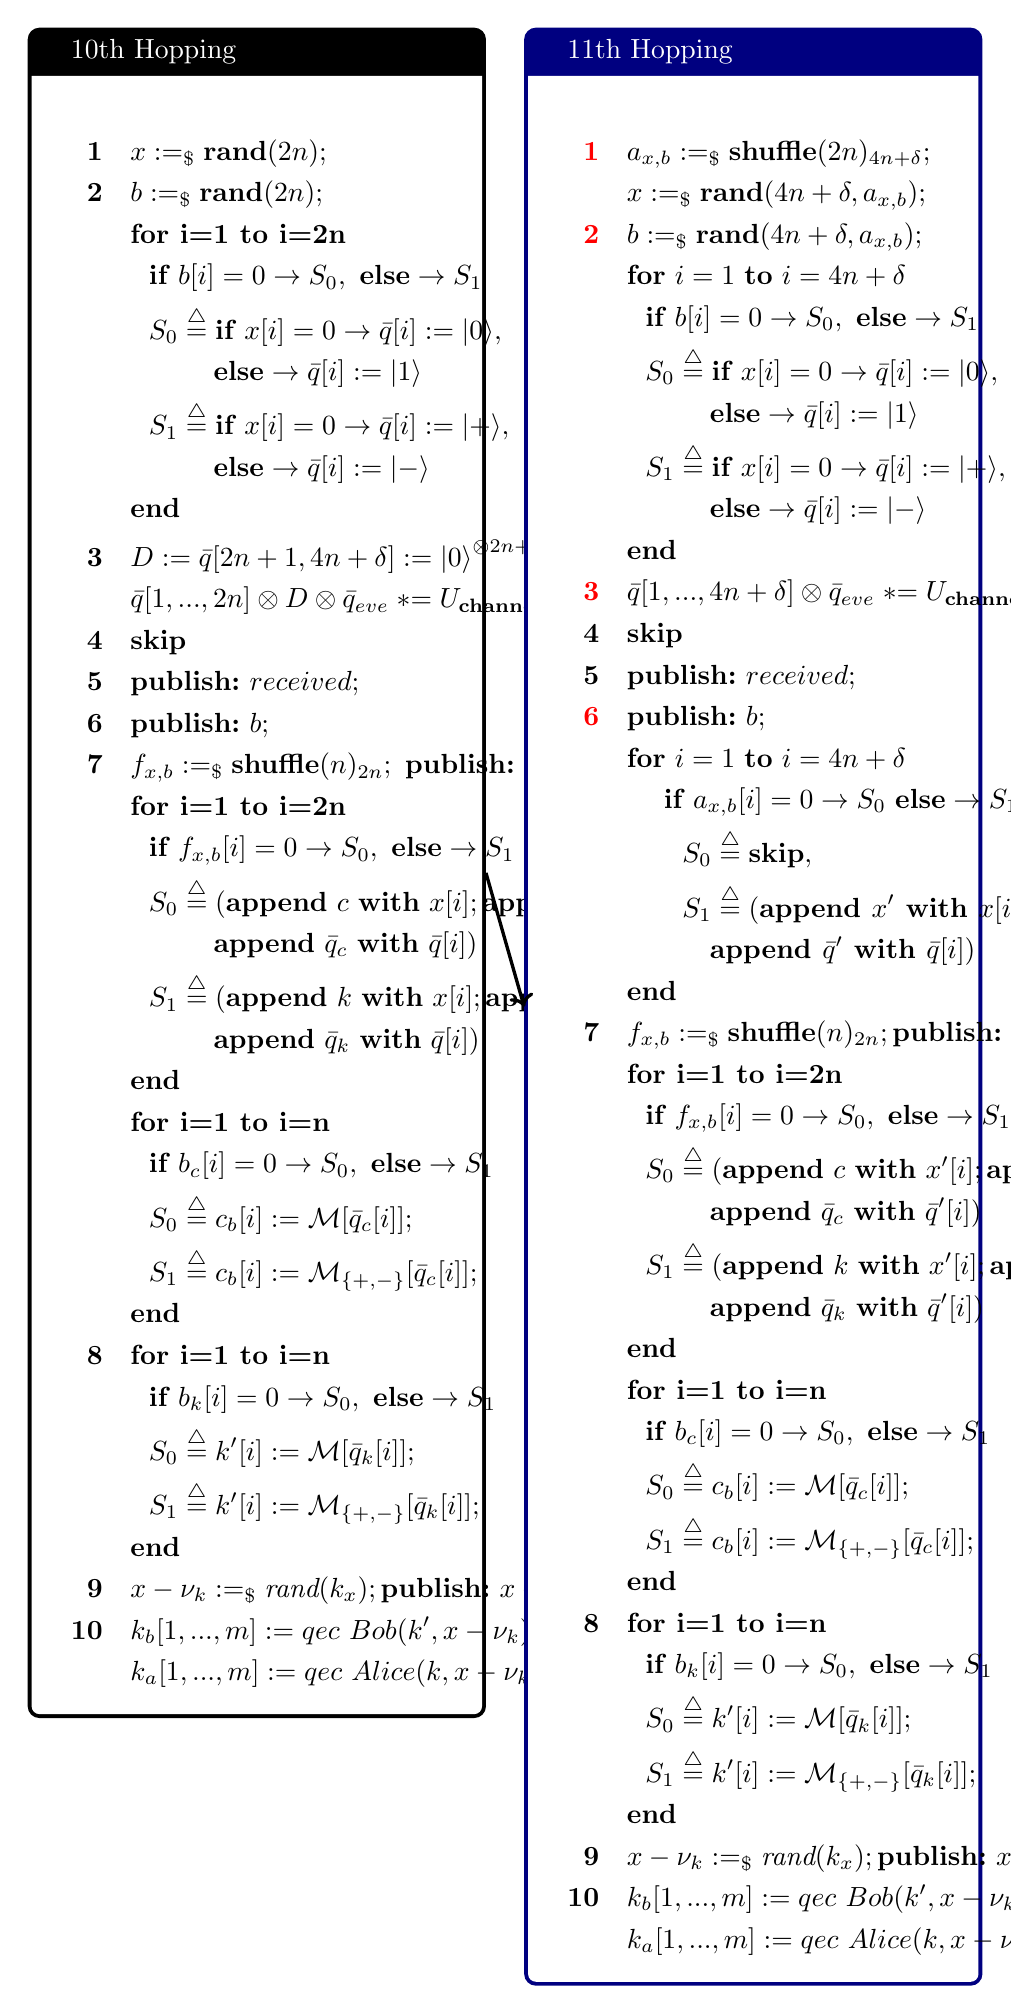
\begin{tikzpicture}[remember picture]

% Left box
\node[anchor=north west,inner sep=0pt,outer sep=0pt] (leftbox) at (0,0) {
\begin{minipage}[t]{0.48\textwidth}
\begin{tcolorbox}[colframe=black!50!black, colback=white, title=10th Hopping, width=\textwidth]
\begin{align*}
    \textbf{{1}} \quad 
    &x :=_\$ \textbf{rand}(2n); \\ 
    \textbf{{2}}\quad 
    & b :=_\$ \textbf{rand}(2n); \\
    &\textbf{for~i=1~to~i=2n}\\
    &~~ \textbf{if }  b[i] = 0 \rightarrow S_{0},~\textbf{else}\rightarrow S_{1}\\
    &~~ S_{0}\stackrel{\triangle}{=}\textbf{if }  x[i] = 0 \rightarrow \bar{q}[i] := |0\rangle,\\ &~~~~~~~~~\textbf{else}   \rightarrow \bar{q}[i] := |1\rangle\\
    &~~ S_{1}\stackrel{\triangle}{=}\textbf{if }  x[i] = 0 \rightarrow \bar{q}[i] := |+\rangle,\\ &~~~~~~~~~\textbf{else}   \rightarrow \bar{q}[i] := |-\rangle\\
    &\textbf{end}\\
    \textbf{{3}} 
    \quad & {D}:= \bar{q}[2n+1,4n+\delta]:=\ket{0}^{\otimes 2n+\delta};\\     &\bar{q}[1,...,2n]\otimes {D} \otimes \bar{q}_{eve} \asteq U_{\textbf{channel}}; \\
    \textbf{{4}} \quad &\textbf{skip} \\ 
    \textbf{{5}} \quad & \textbf{publish:}~ received;\\
    \textbf{{6}} \quad & \textbf{publish:}~b;\\
    \textbf{{7}} 
    \quad &f_{x,b}:=_\$\textbf{shuffle}(n)_{2n}; ~ \textbf{publish:}~ f_{x,b};\\
    &\textbf{for~i=1~to~i=2n}\\
    &~~ \textbf{if }  f_{x,b}[i] = 0 \rightarrow S_{0},~\textbf{else}\rightarrow S_{1}\\
    &~~ S_{0}\stackrel{\triangle}{=}(\textbf{append}~c~\textbf{with}~x[i];\textbf{append}~b_c~\textbf{with}~b[i];\\
    &\qquad\quad\textbf{append}~\bar{q}_c~\textbf{with}~\bar{q}[i])\\
    &~~ S_{1}\stackrel{\triangle}{=}(\textbf{append}~k~\textbf{with}~x[i];\textbf{append}~b_k~\textbf{with}~b[i];\\
    &\qquad\quad\textbf{append}~\bar{q}_k~\textbf{with}~\bar{q}[i])\\
    &\textbf{end}\\
    &\textbf{for~i=1~to~i=n}\\
    &~~ \textbf{if }  b_c[i] = 0 \rightarrow S_{0},~\textbf{else}\rightarrow S_{1}\\
    &~~ S_{0}\stackrel{\triangle}{=}c_b[i]:= \mathcal{M} [\bar{q}_c[i]];\\
    &~~ S_{1}\stackrel{\triangle}{=}c_b[i]:= \mathcal{M}_{\{+,-\}} [\bar{q}_c[i]];\\
    &\textbf{end}\\
    \textbf{{8}}\quad 
    &\textbf{for~i=1~to~i=n}\\
    &~~ \textbf{if }  b_k[i] = 0 \rightarrow S_{0},~\textbf{else}\rightarrow S_{1}\\
    &~~ S_{0}\stackrel{\triangle}{=}k'[i]:= \mathcal{M} [\bar{q}_k[i]];\\
    &~~ S_{1}\stackrel{\triangle}{=}k'[i]:= \mathcal{M}_{\{+,-\}} [\bar{q}_k[i]];\\
    &\textbf{end}\\
    \textbf{{9}} \quad & x-\nu_k :=_\$ \textit{rand}(k_x); \textbf{publish:}~ x-\nu_k;\\
    \textbf{{10}} \quad 
    &k_b[1,...,m]:=qec~Bob(k',x-\nu_k)\\
    &k_a[1,...,m]:=qec~Alice(k,x-\nu_k)
\end{align*}
\end{tcolorbox}
\end{minipage}
};

% Right box
\node[anchor=north west,inner sep=0pt,outer sep=0pt] (rightbox) at (0.52\textwidth,0) {
\begin{minipage}[t]{0.48\textwidth}
\begin{tcolorbox}[colframe=blue!50!black, colback=white, title=11th Hopping, width=\textwidth]
\begin{align*}
    \textbf{\textcolor{red}{1}} \quad 
    & a_{x,b}:=_\$\textbf{shuffle}(2n)_{4n+\delta};\\
    &x :=_\$ \textbf{rand}(4n+\delta,a_{x,b}); \\ 
    \textbf{\textcolor{red}{2}}\quad 
    & b :=_\$ \textbf{rand}(4n+\delta,a_{x,b}); \\
    &\textbf{for}~i=1~\textbf{to}~i=4n+\delta\\
    &~~ \textbf{if }  b[i] = 0 \rightarrow S_{0},~\textbf{else}\rightarrow S_{1}\\
    &~~ S_{0}\stackrel{\triangle}{=}\textbf{if }  x[i] = 0 \rightarrow \bar{q}[i] := |0\rangle,\\ &~~~~~~~~~\textbf{else}   \rightarrow \bar{q}[i] := |1\rangle\\
    &~~ S_{1}\stackrel{\triangle}{=}\textbf{if }  x[i] = 0 \rightarrow \bar{q}[i] := |+\rangle,\\ &~~~~~~~~~\textbf{else}   \rightarrow \bar{q}[i] := |-\rangle\\
    &\textbf{end}\\
    \textbf{\textcolor{red}{3}} 
    \quad & \bar{q}[1,...,4n+\delta] \otimes \bar{q}_{eve} \asteq U_{\textbf{channel}}; \\
    \textbf{{4}} \quad &\textbf{skip} \\ 
    \textbf{{5}} \quad & \textbf{publish:}~ received;\\
    \textbf{\textcolor{red}{6}} \quad & \textbf{publish:}~b;\\
    &\textbf{for}~i=1~\textbf{to}~i=4n+\delta\\
    &~~~~ \textbf{if }  a_{x,b}[i] = 0 \rightarrow S_{0} ~\textbf{else} \rightarrow S_{1} ,\\
    &~~~~~~S_{0}\stackrel{\triangle}{=}\textbf{skip},\\
    &~~~~~~S_{1}\stackrel{\triangle}{=}(\textbf{append } x' \textbf{ with } x[i];\textbf{append } b' \textbf{ with } b[i];\\
    &\qquad\quad\textbf{append } \bar{q}' \textbf{ with } \bar{q}[i])\\
    &\textbf{end}\\
    \textbf{{7}} 
    \quad & f_{x,b}:=_\$\textbf{shuffle}(n)_{2n}; \textbf{publish:}~ f_{x,b};\\
    &\textbf{for~i=1~to~i=2n}\\
    &~~ \textbf{if }  f_{x,b}[i] = 0 \rightarrow S_{0},~\textbf{else}\rightarrow S_{1}\\
    &~~ S_{0}\stackrel{\triangle}{=}(\textbf{append}~c~\textbf{with}~x'[i];\textbf{append}~b_c~\textbf{with}~b'[i];\\
    &\qquad\quad\textbf{append}~\bar{q}_c~\textbf{with}~\bar{q}'[i])\\
    &~~ S_{1}\stackrel{\triangle}{=}(\textbf{append}~k~\textbf{with}~x'[i];\textbf{append}~b_k~\textbf{with}~b'[i];\\
    &\qquad\quad\textbf{append}~\bar{q}_k~\textbf{with}~\bar{q}'[i])\\
    &\textbf{end}\\
    &\textbf{for~i=1~to~i=n}\\
    &~~ \textbf{if }  b_c[i] = 0 \rightarrow S_{0},~\textbf{else}\rightarrow S_{1}\\
    &~~ S_{0}\stackrel{\triangle}{=}c_b[i]:= \mathcal{M} [\bar{q}_c[i]];\\
    &~~ S_{1}\stackrel{\triangle}{=}c_b[i]:= \mathcal{M}_{\{+,-\}} [\bar{q}_c[i]];\\
    &\textbf{end}\\
    \textbf{{8}}\quad 
    &\textbf{for~i=1~to~i=n}\\
    &~~ \textbf{if }  b_k[i] = 0 \rightarrow S_{0},~\textbf{else}\rightarrow S_{1}\\
    &~~ S_{0}\stackrel{\triangle}{=}k'[i]:= \mathcal{M} [\bar{q}_k[i]];\\
    &~~ S_{1}\stackrel{\triangle}{=}k'[i]:= \mathcal{M}_{\{+,-\}} [\bar{q}_k[i]];\\
    &\textbf{end}\\
    \textbf{{9}} \quad & x-\nu_k :=_\$ \textit{rand}(k_x); \textbf{publish:}~ x-\nu_k;\\
    \textbf{{10}} \quad 
    &k_b[1,...,m]:=qec~Bob(k',x-\nu_k)\\
    &k_a[1,...,m]:=qec~Alice(k,x-\nu_k)
\end{align*}
\end{tcolorbox}
\end{minipage}
};

% Draw arrow between boxes
\draw[->, very thick] (leftbox.east) -- node[above]{} (rightbox.west);

\end{tikzpicture}
\newpage

\noindent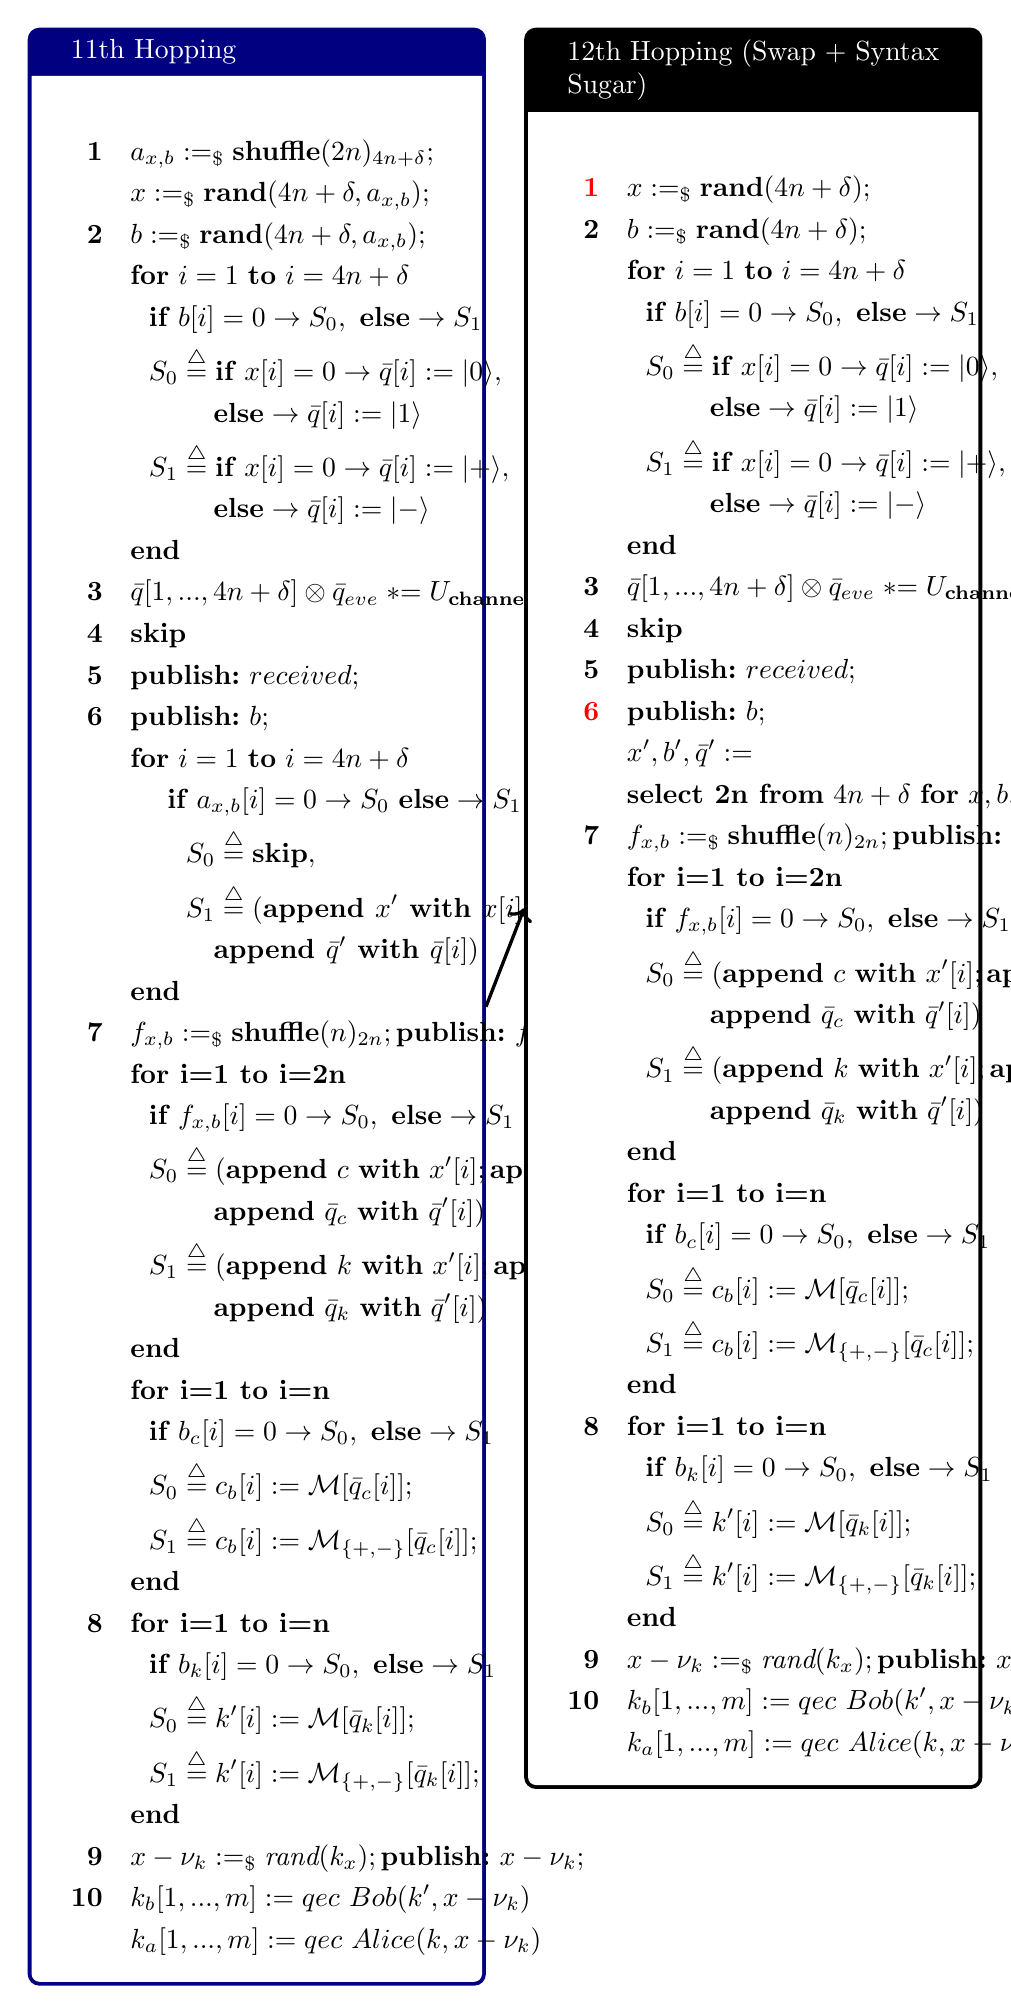
\begin{tikzpicture}[remember picture]

% Left box
\node[anchor=north west,inner sep=0pt,outer sep=0pt] (leftbox) at (0,0) {
\begin{minipage}[t]{0.48\textwidth}
\begin{tcolorbox}[colframe=blue!50!black, colback=white, title=11th Hopping, width=\textwidth]
\begin{align*}
    \textbf{{1}} \quad 
    & a_{x,b}:=_\$\textbf{shuffle}(2n)_{4n+\delta};\\
    &x :=_\$ \textbf{rand}(4n+\delta,a_{x,b}); \\ 
    \textbf{{2}}\quad 
    & b :=_\$ \textbf{rand}(4n+\delta,a_{x,b}); \\
    &\textbf{for}~i=1~\textbf{to}~i=4n+\delta\\
    &~~ \textbf{if }  b[i] = 0 \rightarrow S_{0},~\textbf{else}\rightarrow S_{1}\\
    &~~ S_{0}\stackrel{\triangle}{=}\textbf{if }  x[i] = 0 \rightarrow \bar{q}[i] := |0\rangle,\\ &~~~~~~~~~\textbf{else}   \rightarrow \bar{q}[i] := |1\rangle\\
    &~~ S_{1}\stackrel{\triangle}{=}\textbf{if }  x[i] = 0 \rightarrow \bar{q}[i] := |+\rangle,\\ &~~~~~~~~~\textbf{else}   \rightarrow \bar{q}[i] := |-\rangle\\
    &\textbf{end}\\
    \textbf{{3}} 
    \quad & \bar{q}[1,...,4n+\delta] \otimes \bar{q}_{eve} \asteq U_{\textbf{channel}}; \\
    \textbf{{4}} \quad &\textbf{skip} \\ 
    \textbf{{5}} \quad & \textbf{publish:}~ received;\\
    \textbf{{6}} \quad & \textbf{publish:}~b;\\
    &\textbf{for}~i=1~\textbf{to}~i=4n+\delta\\
    &~~~~ \textbf{if }  a_{x,b}[i] = 0 \rightarrow S_{0} ~\textbf{else} \rightarrow S_{1} ,\\
    &~~~~~~S_{0}\stackrel{\triangle}{=}\textbf{skip},\\
    &~~~~~~S_{1}\stackrel{\triangle}{=}(\textbf{append } x' \textbf{ with } x[i];\textbf{append } b' \textbf{ with } b[i];\\
    &\qquad\quad\textbf{append } \bar{q}' \textbf{ with } \bar{q}[i])\\
    &\textbf{end}\\
    \textbf{{7}} 
    \quad & f_{x,b}:=_\$\textbf{shuffle}(n)_{2n}; \textbf{publish:}~ f_{x,b};\\
    &\textbf{for~i=1~to~i=2n}\\
    &~~ \textbf{if }  f_{x,b}[i] = 0 \rightarrow S_{0},~\textbf{else}\rightarrow S_{1}\\
    &~~ S_{0}\stackrel{\triangle}{=}(\textbf{append}~c~\textbf{with}~x'[i];\textbf{append}~b_c~\textbf{with}~b'[i];\\
    &\qquad\quad\textbf{append}~\bar{q}_c~\textbf{with}~\bar{q}'[i])\\
    &~~ S_{1}\stackrel{\triangle}{=}(\textbf{append}~k~\textbf{with}~x'[i];\textbf{append}~b_k~\textbf{with}~b'[i];\\
    &\qquad\quad\textbf{append}~\bar{q}_k~\textbf{with}~\bar{q}'[i])\\
    &\textbf{end}\\
    &\textbf{for~i=1~to~i=n}\\
    &~~ \textbf{if }  b_c[i] = 0 \rightarrow S_{0},~\textbf{else}\rightarrow S_{1}\\
    &~~ S_{0}\stackrel{\triangle}{=}c_b[i]:= \mathcal{M} [\bar{q}_c[i]];\\
    &~~ S_{1}\stackrel{\triangle}{=}c_b[i]:= \mathcal{M}_{\{+,-\}} [\bar{q}_c[i]];\\
    &\textbf{end}\\
    \textbf{{8}}\quad 
    &\textbf{for~i=1~to~i=n}\\
    &~~ \textbf{if }  b_k[i] = 0 \rightarrow S_{0},~\textbf{else}\rightarrow S_{1}\\
    &~~ S_{0}\stackrel{\triangle}{=}k'[i]:= \mathcal{M} [\bar{q}_k[i]];\\
    &~~ S_{1}\stackrel{\triangle}{=}k'[i]:= \mathcal{M}_{\{+,-\}} [\bar{q}_k[i]];\\
    &\textbf{end}\\
    \textbf{{9}} \quad & x-\nu_k :=_\$ \textit{rand}(k_x); \textbf{publish:}~ x-\nu_k;\\
    \textbf{{10}} \quad 
    &k_b[1,...,m]:=qec~Bob(k',x-\nu_k)\\
    &k_a[1,...,m]:=qec~Alice(k,x-\nu_k)
\end{align*}
\end{tcolorbox}
\end{minipage}
};

% Right box
\node[anchor=north west,inner sep=0pt,outer sep=0pt] (rightbox) at (0.52\textwidth,0) {
\begin{minipage}[t]{0.48\textwidth}
\begin{tcolorbox}[colframe=black!50!black, colback=white, title=12th Hopping (Swap + Syntax Sugar), width=\textwidth]
\begin{align*}
    \textbf{\textcolor{red}{1}} \quad 
    & x :=_\$ \textbf{rand}(4n+\delta); \\ 
    \textbf{{2}}\quad 
    & b :=_\$ \textbf{rand}(4n+\delta); \\
    &\textbf{for}~i=1~\textbf{to}~i=4n+\delta\\
    &~~ \textbf{if }  b[i] = 0 \rightarrow S_{0},~\textbf{else}\rightarrow S_{1}\\
    &~~ S_{0}\stackrel{\triangle}{=}\textbf{if }  x[i] = 0 \rightarrow \bar{q}[i] := |0\rangle,\\ &~~~~~~~~~\textbf{else}   \rightarrow \bar{q}[i] := |1\rangle\\
    &~~ S_{1}\stackrel{\triangle}{=}\textbf{if }  x[i] = 0 \rightarrow \bar{q}[i] := |+\rangle,\\ &~~~~~~~~~\textbf{else}   \rightarrow \bar{q}[i] := |-\rangle\\
    &\textbf{end}\\
    \textbf{{3}} 
    \quad & \bar{q}[1,...,4n+\delta] \otimes \bar{q}_{eve} \asteq U_{\textbf{channel}}; \\
    \textbf{{4}} \quad &\textbf{skip} \\ 
    \textbf{{5}} \quad & \textbf{publish:}~ received;\\
    \textbf{\textcolor{red}{6}} \quad & \textbf{publish:}~b;\\
     &x',b',\bar{q}':=\\&\textbf{select 2n from}~4n+\delta ~\textbf{for}~ x,b,\bar{q};\\ 
    \textbf{{7}} 
    \quad & f_{x,b}:=_\$\textbf{shuffle}(n)_{2n}; \textbf{publish:}~ f_{x,b};\\
    &\textbf{for~i=1~to~i=2n}\\
    &~~ \textbf{if }  f_{x,b}[i] = 0 \rightarrow S_{0},~\textbf{else}\rightarrow S_{1}\\
    &~~ S_{0}\stackrel{\triangle}{=}(\textbf{append}~c~\textbf{with}~x'[i];\textbf{append}~b_c~\textbf{with}~b'[i];\\
    &\qquad\quad\textbf{append}~\bar{q}_c~\textbf{with}~\bar{q}'[i])\\
    &~~ S_{1}\stackrel{\triangle}{=}(\textbf{append}~k~\textbf{with}~x'[i];\textbf{append}~b_k~\textbf{with}~b'[i];\\
    &\qquad\quad\textbf{append}~\bar{q}_k~\textbf{with}~\bar{q}'[i])\\
    &\textbf{end}\\
    &\textbf{for~i=1~to~i=n}\\
    &~~ \textbf{if }  b_c[i] = 0 \rightarrow S_{0},~\textbf{else}\rightarrow S_{1}\\
    &~~ S_{0}\stackrel{\triangle}{=}c_b[i]:= \mathcal{M} [\bar{q}_c[i]];\\
    &~~ S_{1}\stackrel{\triangle}{=}c_b[i]:= \mathcal{M}_{\{+,-\}} [\bar{q}_c[i]];\\
    &\textbf{end}\\
    \textbf{{8}}\quad 
    &\textbf{for~i=1~to~i=n}\\
    &~~ \textbf{if }  b_k[i] = 0 \rightarrow S_{0},~\textbf{else}\rightarrow S_{1}\\
    &~~ S_{0}\stackrel{\triangle}{=}k'[i]:= \mathcal{M} [\bar{q}_k[i]];\\
    &~~ S_{1}\stackrel{\triangle}{=}k'[i]:= \mathcal{M}_{\{+,-\}} [\bar{q}_k[i]];\\
    &\textbf{end}\\
    \textbf{{9}} \quad & x-\nu_k :=_\$ \textit{rand}(k_x); \textbf{publish:}~ x-\nu_k;\\
    \textbf{{10}} \quad 
    &k_b[1,...,m]:=qec~Bob(k',x-\nu_k)\\
    &k_a[1,...,m]:=qec~Alice(k,x-\nu_k)
\end{align*}
\end{tcolorbox}
\end{minipage}
};

% Draw arrow between boxes
\draw[->, very thick] (leftbox.east) -- node[above]{} (rightbox.west);

\end{tikzpicture}
\newpage

\noindent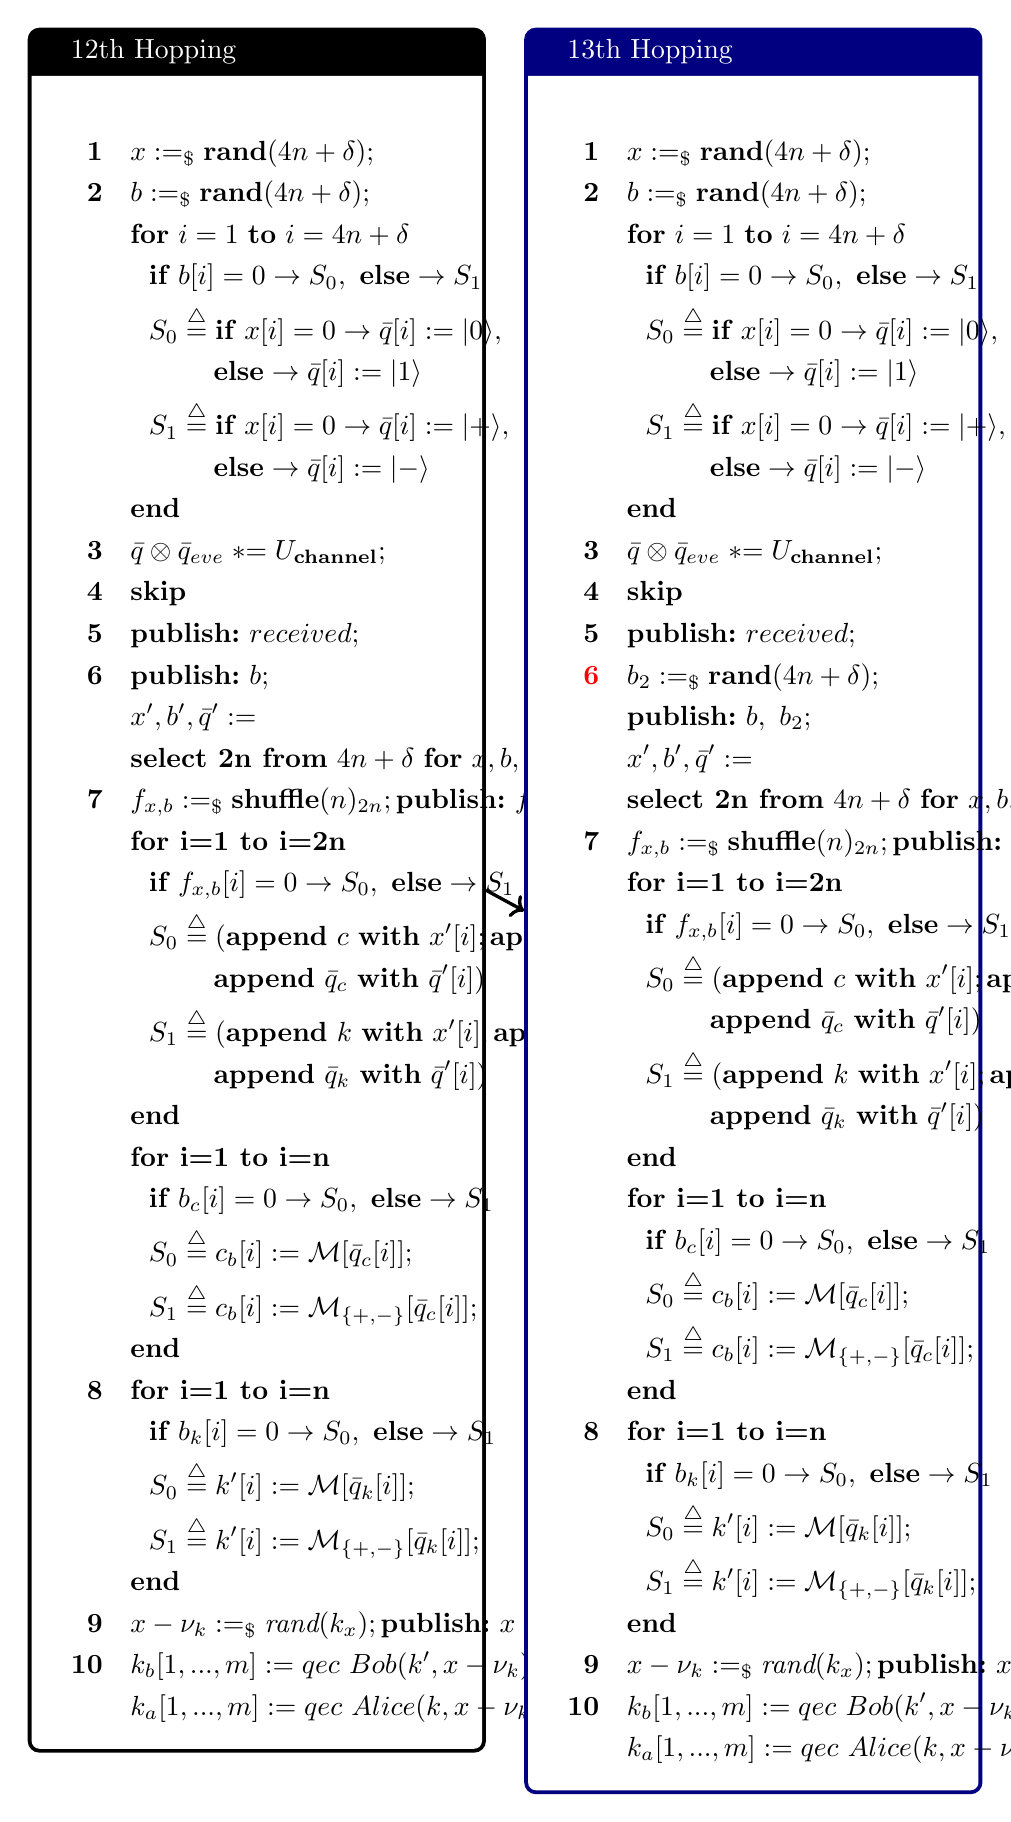
\begin{tikzpicture}[remember picture]

% Left box
\node[anchor=north west,inner sep=0pt,outer sep=0pt] (leftbox) at (0,0) {
\begin{minipage}[t]{0.48\textwidth}
\begin{tcolorbox}[colframe=black!50!black, colback=white, title=12th Hopping, width=\textwidth]
\begin{align*}
    \textbf{{1}} \quad 
    & x :=_\$ \textbf{rand}(4n+\delta); \\ 
    \textbf{{2}}\quad 
    & b :=_\$ \textbf{rand}(4n+\delta); \\
    &\textbf{for}~i=1~\textbf{to}~i=4n+\delta\\
    &~~ \textbf{if }  b[i] = 0 \rightarrow S_{0},~\textbf{else}\rightarrow S_{1}\\
    &~~ S_{0}\stackrel{\triangle}{=}\textbf{if }  x[i] = 0 \rightarrow \bar{q}[i] := |0\rangle,\\ &~~~~~~~~~\textbf{else}   \rightarrow \bar{q}[i] := |1\rangle\\
    &~~ S_{1}\stackrel{\triangle}{=}\textbf{if }  x[i] = 0 \rightarrow \bar{q}[i] := |+\rangle,\\ &~~~~~~~~~\textbf{else}   \rightarrow \bar{q}[i] := |-\rangle\\
    &\textbf{end}\\
    \textbf{{3}} 
    \quad & \bar{q} \otimes \bar{q}_{eve} \asteq U_{\textbf{channel}}; \\
    \textbf{{4}} \quad &\textbf{skip} \\ 
    \textbf{{5}} \quad & \textbf{publish:}~ received;\\
    \textbf{{6}} \quad & \textbf{publish:}~b;\\
     &x',b',\bar{q}':=\\&\textbf{select 2n from}~4n+\delta ~\textbf{for}~ x,b,\bar{q};\\ 
    \textbf{{7}} 
    \quad & f_{x,b}:=_\$\textbf{shuffle}(n)_{2n}; \textbf{publish:}~ f_{x,b};\\
    &\textbf{for~i=1~to~i=2n}\\
    &~~ \textbf{if }  f_{x,b}[i] = 0 \rightarrow S_{0},~\textbf{else}\rightarrow S_{1}\\
    &~~ S_{0}\stackrel{\triangle}{=}(\textbf{append}~c~\textbf{with}~x'[i];\textbf{append}~b_c~\textbf{with}~b'[i];\\
    &\qquad\quad\textbf{append}~\bar{q}_c~\textbf{with}~\bar{q}'[i])\\
    &~~ S_{1}\stackrel{\triangle}{=}(\textbf{append}~k~\textbf{with}~x'[i];\textbf{append}~b_k~\textbf{with}~b'[i];\\
    &\qquad\quad\textbf{append}~\bar{q}_k~\textbf{with}~\bar{q}'[i])\\
    &\textbf{end}\\
    &\textbf{for~i=1~to~i=n}\\
    &~~ \textbf{if }  b_c[i] = 0 \rightarrow S_{0},~\textbf{else}\rightarrow S_{1}\\
    &~~ S_{0}\stackrel{\triangle}{=}c_b[i]:= \mathcal{M} [\bar{q}_c[i]];\\
    &~~ S_{1}\stackrel{\triangle}{=}c_b[i]:= \mathcal{M}_{\{+,-\}} [\bar{q}_c[i]];\\
    &\textbf{end}\\
    \textbf{{8}}\quad 
    &\textbf{for~i=1~to~i=n}\\
    &~~ \textbf{if }  b_k[i] = 0 \rightarrow S_{0},~\textbf{else}\rightarrow S_{1}\\
    &~~ S_{0}\stackrel{\triangle}{=}k'[i]:= \mathcal{M} [\bar{q}_k[i]];\\
    &~~ S_{1}\stackrel{\triangle}{=}k'[i]:= \mathcal{M}_{\{+,-\}} [\bar{q}_k[i]];\\
    &\textbf{end}\\
    \textbf{{9}} \quad & x-\nu_k :=_\$ \textit{rand}(k_x); \textbf{publish:}~ x-\nu_k;\\
    \textbf{{10}} \quad 
    &k_b[1,...,m]:=qec~Bob(k',x-\nu_k)\\
    &k_a[1,...,m]:=qec~Alice(k,x-\nu_k)
\end{align*}
\end{tcolorbox}
\end{minipage}
};

% Right box
\node[anchor=north west,inner sep=0pt,outer sep=0pt] (rightbox) at (0.52\textwidth,0) {
\begin{minipage}[t]{0.48\textwidth}
\begin{tcolorbox}[colframe=blue!50!black, colback=white, title=13th Hopping, width=\textwidth]
\begin{align*}
    \textbf{{1}} \quad 
    & x :=_\$ \textbf{rand}(4n+\delta); \\ 
    \textbf{{2}}\quad 
    & b :=_\$ \textbf{rand}(4n+\delta); \\
    &\textbf{for} ~i=1 ~\textbf{to}~ i=4n+\delta\\
    &~~ \textbf{if }  b[i] = 0 \rightarrow S_{0},~\textbf{else}\rightarrow S_{1}\\
    &~~ S_{0}\stackrel{\triangle}{=}\textbf{if }  x[i] = 0 \rightarrow \bar{q}[i] := |0\rangle,\\ &~~~~~~~~~\textbf{else}   \rightarrow \bar{q}[i] := |1\rangle\\
    &~~ S_{1}\stackrel{\triangle}{=}\textbf{if }  x[i] = 0 \rightarrow \bar{q}[i] := |+\rangle,\\ &~~~~~~~~~\textbf{else}   \rightarrow \bar{q}[i] := |-\rangle\\
    &\textbf{end}\\
    \textbf{{3}} 
    \quad & \bar{q}\otimes \bar{q}_{eve} \asteq U_{\textbf{channel}}; \\
    \textbf{{4}} \quad &\textbf{skip} \\ 
    \textbf{{5}} \quad & \textbf{publish:}~ received;\\
    \textbf{\textcolor{red}{6}} \quad & b_2 :=_\$ \textbf{rand}(4n+\delta); \\
    \quad & \textbf{publish:}~b,~b_2;\\
     &x',b',\bar{q}':=\\&\textbf{select 2n from}~4n+\delta ~\textbf{for}~ x,b,\bar{q};\\
    \textbf{{7}} 
    \quad & f_{x,b}:=_\$\textbf{shuffle}(n)_{2n}; \textbf{publish:}~ f_{x,b};\\
    &\textbf{for~i=1~to~i=2n}\\
    &~~ \textbf{if }  f_{x,b}[i] = 0 \rightarrow S_{0},~\textbf{else}\rightarrow S_{1}\\
    &~~ S_{0}\stackrel{\triangle}{=}(\textbf{append}~c~\textbf{with}~x'[i];\textbf{append}~b_c~\textbf{with}~b'[i];\\
    &\qquad\quad\textbf{append}~\bar{q}_c~\textbf{with}~\bar{q}'[i])\\
    &~~ S_{1}\stackrel{\triangle}{=}(\textbf{append}~k~\textbf{with}~x'[i];\textbf{append}~b_k~\textbf{with}~b'[i];\\
    &\qquad\quad\textbf{append}~\bar{q}_k~\textbf{with}~\bar{q}'[i])\\
    &\textbf{end}\\
    &\textbf{for~i=1~to~i=n}\\
    &~~ \textbf{if }  b_c[i] = 0 \rightarrow S_{0},~\textbf{else}\rightarrow S_{1}\\
    &~~ S_{0}\stackrel{\triangle}{=}c_b[i]:= \mathcal{M} [\bar{q}_c[i]];\\
    &~~ S_{1}\stackrel{\triangle}{=}c_b[i]:= \mathcal{M}_{\{+,-\}} [\bar{q}_c[i]];\\
    &\textbf{end}\\
    \textbf{{8}}\quad 
    &\textbf{for~i=1~to~i=n}\\
    &~~ \textbf{if }  b_k[i] = 0 \rightarrow S_{0},~\textbf{else}\rightarrow S_{1}\\
    &~~ S_{0}\stackrel{\triangle}{=}k'[i]:= \mathcal{M} [\bar{q}_k[i]];\\
    &~~ S_{1}\stackrel{\triangle}{=}k'[i]:= \mathcal{M}_{\{+,-\}} [\bar{q}_k[i]];\\
    &\textbf{end}\\
    \textbf{{9}} \quad & x-\nu_k :=_\$ \textit{rand}(k_x); \textbf{publish:}~ x-\nu_k;\\
    \textbf{{10}} \quad 
    &k_b[1,...,m]:=qec~Bob(k',x-\nu_k)\\
    &k_a[1,...,m]:=qec~Alice(k,x-\nu_k)
\end{align*}
\end{tcolorbox}
\end{minipage}
};

% Draw arrow between boxes
\draw[->, very thick] (leftbox.east) -- node[above]{} (rightbox.west);

\end{tikzpicture}
\newpage


\noindent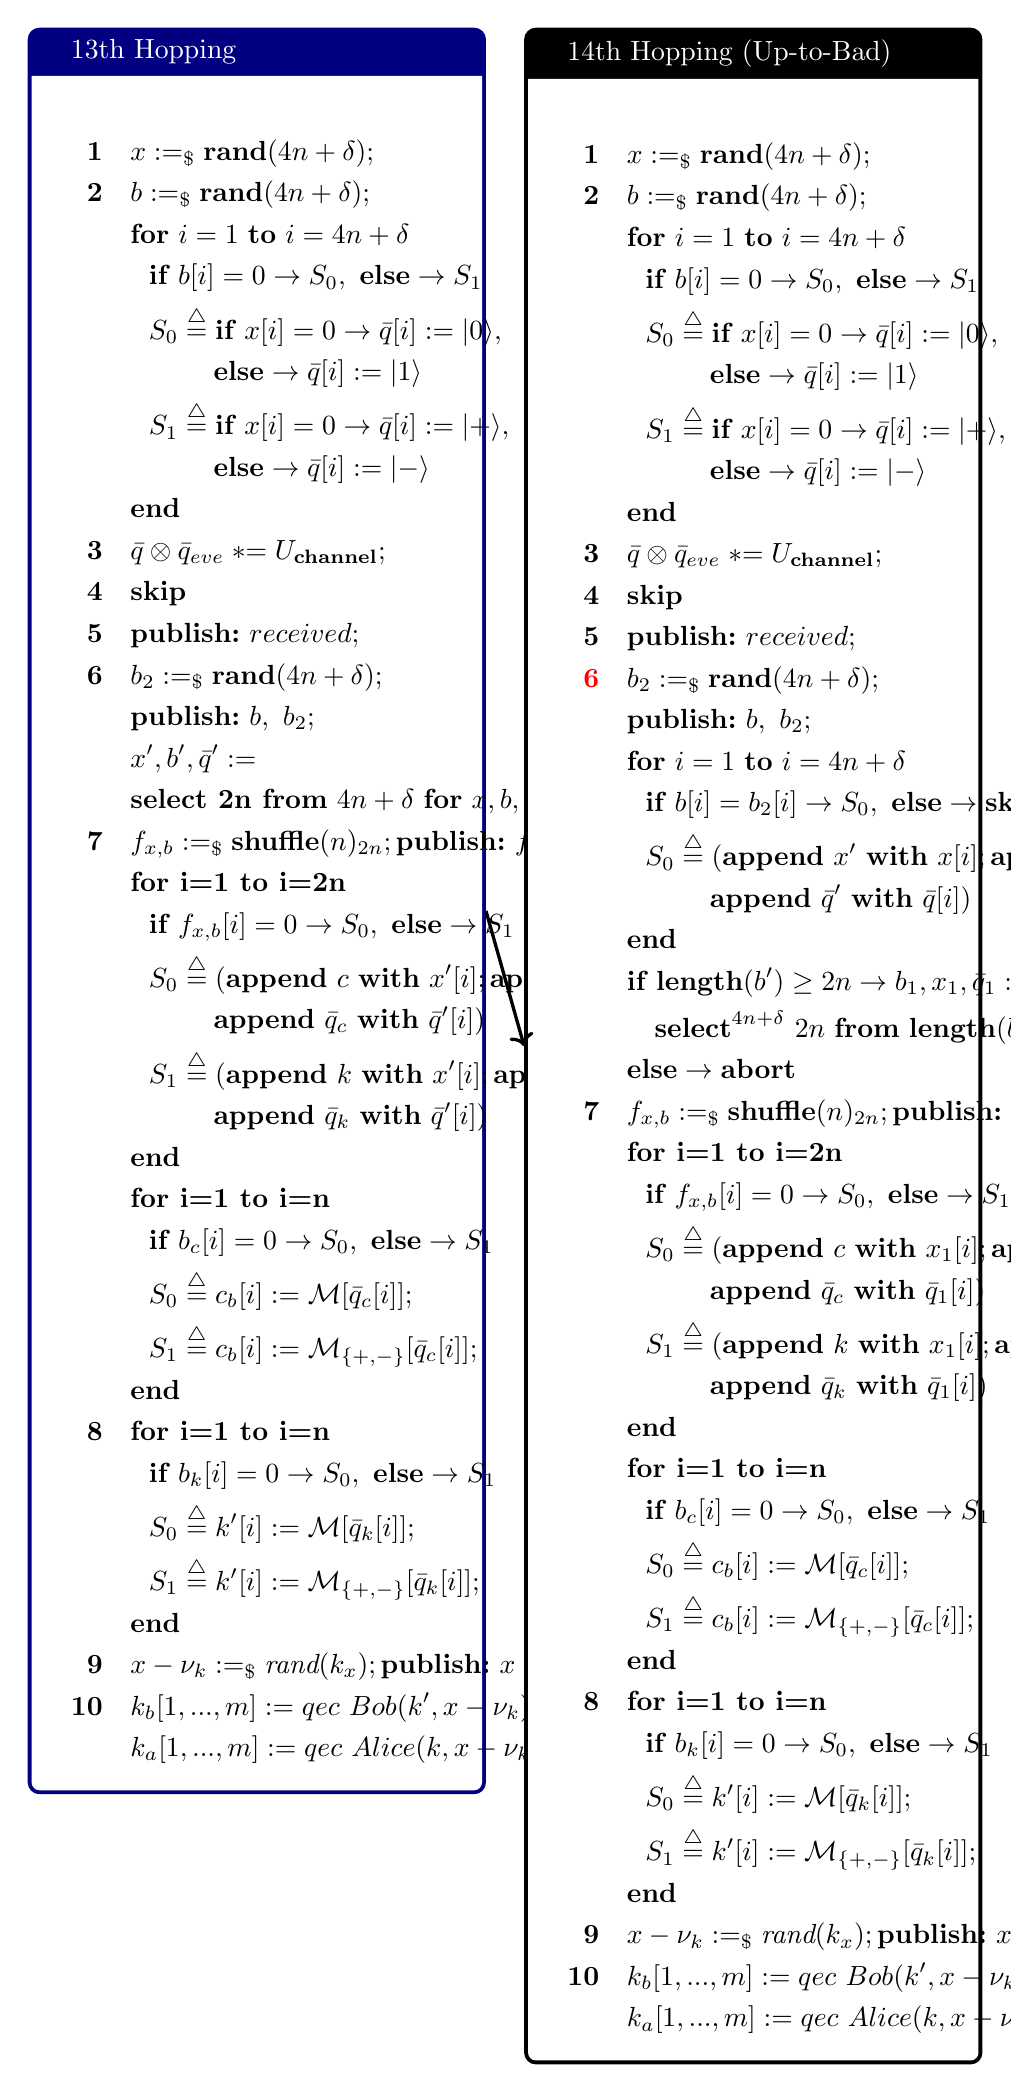
\begin{tikzpicture}[remember picture]

% Left box
\node[anchor=north west,inner sep=0pt,outer sep=0pt] (leftbox) at (0,0) {
\begin{minipage}[t]{0.48\textwidth}
\begin{tcolorbox}[colframe=blue!50!black, colback=white, title=13th Hopping, width=\textwidth]
\begin{align*}
    \textbf{{1}} \quad 
    & x :=_\$ \textbf{rand}(4n+\delta); \\ 
    \textbf{{2}}\quad 
    & b :=_\$ \textbf{rand}(4n+\delta); \\
    &\textbf{for}~i=1~\textbf{to}~i=4n+\delta\\
    &~~ \textbf{if }  b[i] = 0 \rightarrow S_{0},~\textbf{else}\rightarrow S_{1}\\
    &~~ S_{0}\stackrel{\triangle}{=}\textbf{if }  x[i] = 0 \rightarrow \bar{q}[i] := |0\rangle,\\ &~~~~~~~~~\textbf{else}   \rightarrow \bar{q}[i] := |1\rangle\\
    &~~ S_{1}\stackrel{\triangle}{=}\textbf{if }  x[i] = 0 \rightarrow \bar{q}[i] := |+\rangle,\\ &~~~~~~~~~\textbf{else}   \rightarrow \bar{q}[i] := |-\rangle\\
    &\textbf{end}\\
    \textbf{{3}} 
    \quad & \bar{q} \otimes \bar{q}_{eve} \asteq U_{\textbf{channel}}; \\
    \textbf{{4}} \quad &\textbf{skip} \\ 
    \textbf{{5}} \quad & \textbf{publish:}~ received;\\
    \textbf{{6}} \quad & b_2 :=_\$ \textbf{rand}(4n+\delta); \\ \quad & \textbf{publish:}~b,~b_2;\\
     &x',b',\bar{q}':=\\&\textbf{select 2n from}~4n+\delta ~\textbf{for}~ x,b,\bar{q};\\
    \textbf{{7}} 
    \quad & f_{x,b}:=_\$\textbf{shuffle}(n)_{2n}; \textbf{publish:}~ f_{x,b};\\
    &\textbf{for~i=1~to~i=2n}\\
    &~~ \textbf{if }  f_{x,b}[i] = 0 \rightarrow S_{0},~\textbf{else}\rightarrow S_{1}\\
    &~~ S_{0}\stackrel{\triangle}{=}(\textbf{append}~c~\textbf{with}~x'[i];\textbf{append}~b_c~\textbf{with}~b'[i];\\
    &\qquad\quad\textbf{append}~\bar{q}_c~\textbf{with}~\bar{q}'[i])\\
    &~~ S_{1}\stackrel{\triangle}{=}(\textbf{append}~k~\textbf{with}~x'[i];\textbf{append}~b_k~\textbf{with}~b'[i];\\
    &\qquad\quad\textbf{append}~\bar{q}_k~\textbf{with}~\bar{q}'[i])\\
    &\textbf{end}\\
    &\textbf{for~i=1~to~i=n}\\
    &~~ \textbf{if }  b_c[i] = 0 \rightarrow S_{0},~\textbf{else}\rightarrow S_{1}\\
    &~~ S_{0}\stackrel{\triangle}{=}c_b[i]:= \mathcal{M} [\bar{q}_c[i]];\\
    &~~ S_{1}\stackrel{\triangle}{=}c_b[i]:= \mathcal{M}_{\{+,-\}} [\bar{q}_c[i]];\\
    &\textbf{end}\\
    \textbf{{8}}\quad 
    &\textbf{for~i=1~to~i=n}\\
    &~~ \textbf{if }  b_k[i] = 0 \rightarrow S_{0},~\textbf{else}\rightarrow S_{1}\\
    &~~ S_{0}\stackrel{\triangle}{=}k'[i]:= \mathcal{M} [\bar{q}_k[i]];\\
    &~~ S_{1}\stackrel{\triangle}{=}k'[i]:= \mathcal{M}_{\{+,-\}} [\bar{q}_k[i]];\\
    &\textbf{end}\\
    \textbf{{9}} \quad & x-\nu_k :=_\$ \textit{rand}(k_x); \textbf{publish:}~ x-\nu_k;\\
    \textbf{{10}} \quad 
    &k_b[1,...,m]:=qec~Bob(k',x-\nu_k)\\
    &k_a[1,...,m]:=qec~Alice(k,x-\nu_k)
\end{align*}
\end{tcolorbox}
\end{minipage}
};

% Right box
\node[anchor=north west,inner sep=0pt,outer sep=0pt] (rightbox) at (0.52\textwidth,0) {
\begin{minipage}[t]{0.48\textwidth}
\begin{tcolorbox}[colframe=black!50!black, colback=white, title=14th Hopping (Up-to-Bad), width=\textwidth]
\begin{align*}
    \textbf{{1}} \quad 
    &x :=_\$ \textbf{rand}(4n+\delta); \\ 
    \textbf{{2}}\quad 
    & b :=_\$ \textbf{rand}(4n+\delta); \\
    &\textbf{for} ~i=1 ~\textbf{to}~ i=4n+\delta\\
    &~~ \textbf{if }  b[i] = 0 \rightarrow S_{0},~\textbf{else}\rightarrow S_{1}\\
    &~~ S_{0}\stackrel{\triangle}{=}\textbf{if }  x[i] = 0 \rightarrow \bar{q}[i] := |0\rangle,\\ &~~~~~~~~~\textbf{else}   \rightarrow \bar{q}[i] := |1\rangle\\
    &~~ S_{1}\stackrel{\triangle}{=}\textbf{if }  x[i] = 0 \rightarrow \bar{q}[i] := |+\rangle,\\ &~~~~~~~~~\textbf{else}   \rightarrow \bar{q}[i] := |-\rangle\\
    &\textbf{end}\\
    \textbf{{3}} 
    \quad & \bar{q}\otimes \bar{q}_{eve} \asteq U_{\textbf{channel}}; \\
    \textbf{{4}} \quad &\textbf{skip} \\ 
    \textbf{{5}} \quad & \textbf{publish:}~ received;\\
    \textbf{\textcolor{red}{6}} \quad & b_2 :=_\$ \textbf{rand}(4n+\delta); \\
    \quad 
    &\textbf{publish:}~b,~b_2;\\
    &\textbf{for} ~i=1 ~\textbf{to} ~i=4n+\delta\\
    &~~ \textbf{if } b[i]= b_2[i] \rightarrow S_{0},~\textbf{else}\rightarrow\textbf{skip} \\
    &~~ S_{0}\stackrel{\triangle}{=}(\textbf{append}~x'~\textbf{with}~x[i];\textbf{append}~b'~\textbf{with}~b[i];\\
    &\qquad\quad\textbf{append}~\bar{q}'~\textbf{with}~\bar{q}[i])\\
    &\textbf{end}\\
    &{\textbf{if }} \textbf{length} (b')\geq 2n\rightarrow b_1,x_1,\bar{q}_1:=\\&\quad\textbf{select}^{4n+\delta}~2n~\textbf{from}~\textbf{length}(b')~\textbf{for}~b',x',\bar{q}',\\
    & \textbf{else}\rightarrow\textbf{abort}\\
    \textbf{{7}} 
    \quad & f_{x,b}:=_\$\textbf{shuffle}(n)_{2n}; \textbf{publish:}~ f_{x,b};\\
    &\textbf{for~i=1~to~i=2n}\\
    &~~ \textbf{if }  f_{x,b}[i] = 0 \rightarrow S_{0},~\textbf{else}\rightarrow S_{1}\\
    &~~ S_{0}\stackrel{\triangle}{=}(\textbf{append}~c~\textbf{with}~x_1[i];\textbf{append}~b_c~\textbf{with}~b_1[i];\\
    &\qquad\quad\textbf{append}~\bar{q}_c~\textbf{with}~\bar{q}_1[i])\\
    &~~ S_{1}\stackrel{\triangle}{=}(\textbf{append}~k~\textbf{with}~x_1[i];\textbf{append}~b_k~\textbf{with}~b_1[i];\\
    &\qquad\quad\textbf{append}~\bar{q}_k~\textbf{with}~\bar{q}_1[i])\\
    &\textbf{end}\\
    &\textbf{for~i=1~to~i=n}\\
    &~~ \textbf{if }  b_c[i] = 0 \rightarrow S_{0},~\textbf{else}\rightarrow S_{1}\\
    &~~ S_{0}\stackrel{\triangle}{=}c_b[i]:= \mathcal{M} [\bar{q}_c[i]];\\
    &~~ S_{1}\stackrel{\triangle}{=}c_b[i]:= \mathcal{M}_{\{+,-\}} [\bar{q}_c[i]];\\
    &\textbf{end}\\
    \textbf{{8}}\quad 
    &\textbf{for~i=1~to~i=n}\\
    &~~ \textbf{if }  b_k[i] = 0 \rightarrow S_{0},~\textbf{else}\rightarrow S_{1}\\
    &~~ S_{0}\stackrel{\triangle}{=}k'[i]:= \mathcal{M} [\bar{q}_k[i]];\\
    &~~ S_{1}\stackrel{\triangle}{=}k'[i]:= \mathcal{M}_{\{+,-\}} [\bar{q}_k[i]];\\
    &\textbf{end}\\
    \textbf{{9}} \quad & x-\nu_k :=_\$ \textit{rand}(k_x); \textbf{publish:}~ x-\nu_k;\\
    \textbf{{10}} \quad 
    &k_b[1,...,m]:=qec~Bob(k',x-\nu_k)\\
    &k_a[1,...,m]:=qec~Alice(k,x-\nu_k)
\end{align*}
\end{tcolorbox}
\end{minipage}
};

% Draw arrow between boxes
\draw[->, very thick] (leftbox.east) -- node[above]{} (rightbox.west);

\end{tikzpicture}
\newpage

\noindent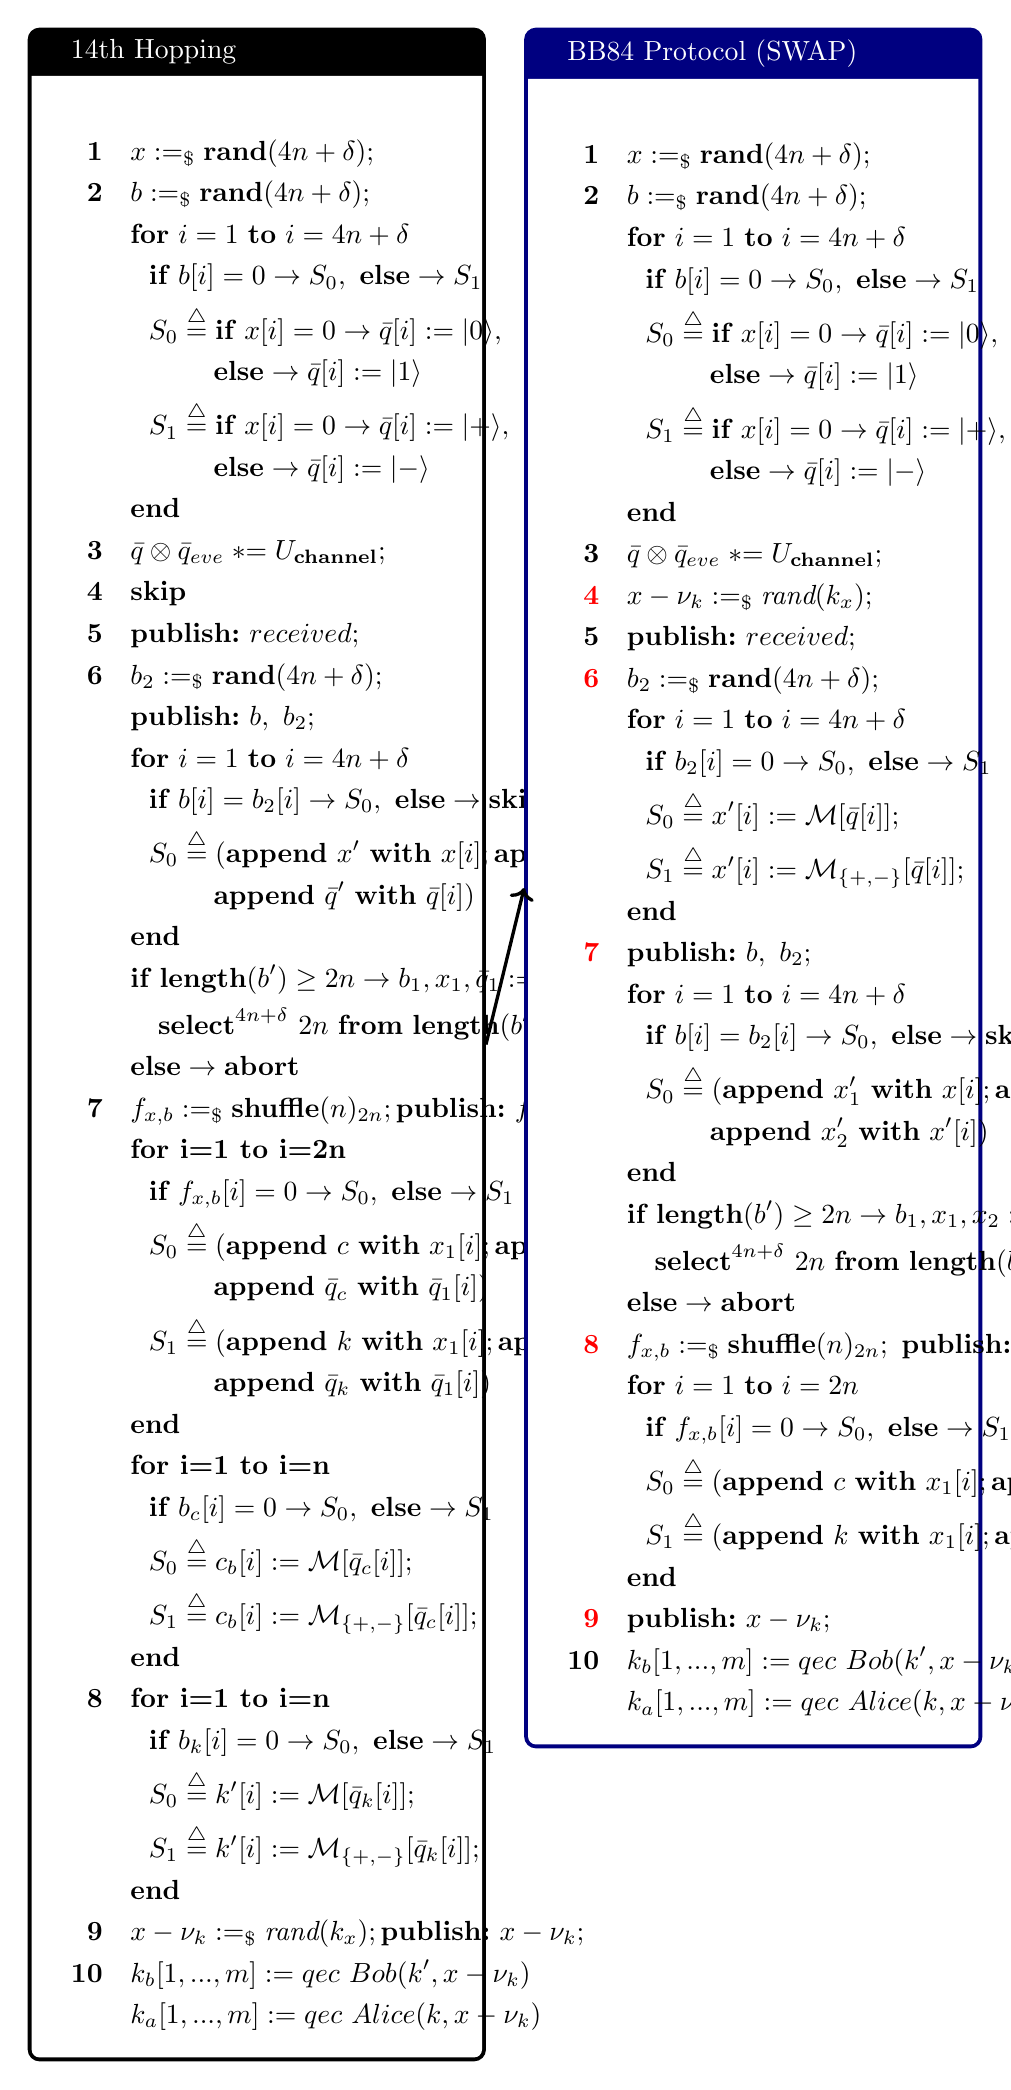
\begin{tikzpicture}[remember picture]

% Left box
\node[anchor=north west,inner sep=0pt,outer sep=0pt] (leftbox) at (0,0) {
\begin{minipage}[t]{0.48\textwidth}
\begin{tcolorbox}[colframe=black!50!black, colback=white, title=14th Hopping, width=\textwidth]
\begin{align*}
    \textbf{{1}} \quad 
    &x :=_\$ \textbf{rand}(4n+\delta); \\ 
    \textbf{{2}}\quad 
    & b :=_\$ \textbf{rand}(4n+\delta); \\
    &\textbf{for} ~i=1 ~\textbf{to}~ i=4n+\delta\\
    &~~ \textbf{if }  b[i] = 0 \rightarrow S_{0},~\textbf{else}\rightarrow S_{1}\\
    &~~ S_{0}\stackrel{\triangle}{=}\textbf{if }  x[i] = 0 \rightarrow \bar{q}[i] := |0\rangle,\\ &~~~~~~~~~\textbf{else}   \rightarrow \bar{q}[i] := |1\rangle\\
    &~~ S_{1}\stackrel{\triangle}{=}\textbf{if }  x[i] = 0 \rightarrow \bar{q}[i] := |+\rangle,\\ &~~~~~~~~~\textbf{else}   \rightarrow \bar{q}[i] := |-\rangle\\
    &\textbf{end}\\
    \textbf{{3}} 
    \quad & \bar{q}\otimes \bar{q}_{eve} \asteq U_{\textbf{channel}}; \\
    \textbf{{4}} \quad &\textbf{skip} \\ 
    \textbf{{5}} \quad & \textbf{publish:}~ received;\\
    \textbf{{6}} \quad & b_2 :=_\$ \textbf{rand}(4n+\delta); \\
    \quad 
    &\textbf{publish:}~b,~b_2;\\
    &\textbf{for} ~i=1 ~\textbf{to} ~i=4n+\delta\\
    &~~ \textbf{if } b[i]= b_2[i] \rightarrow S_{0},~\textbf{else}\rightarrow\textbf{skip} \\
    &~~ S_{0}\stackrel{\triangle}{=}(\textbf{append}~x'~\textbf{with}~x[i];\textbf{append}~b'~\textbf{with}~b[i];\\
    &\qquad\quad\textbf{append}~\bar{q}'~\textbf{with}~\bar{q}[i])\\
    &\textbf{end}\\
    &{\textbf{if }} \textbf{length} (b')\geq 2n\rightarrow b_1,x_1,\bar{q}_1:=\\&\quad\textbf{select}^{4n+\delta}~2n~\textbf{from}~\textbf{length}(b')~\textbf{for}~b',x',\bar{q}',\\
    & \textbf{else}\rightarrow\textbf{abort}\\
    \textbf{{7}} 
    \quad & f_{x,b}:=_\$\textbf{shuffle}(n)_{2n}; \textbf{publish:}~ f_{x,b};\\
    &\textbf{for~i=1~to~i=2n}\\
    &~~ \textbf{if }  f_{x,b}[i] = 0 \rightarrow S_{0},~\textbf{else}\rightarrow S_{1}\\
    &~~ S_{0}\stackrel{\triangle}{=}(\textbf{append}~c~\textbf{with}~x_1[i];\textbf{append}~b_c~\textbf{with}~b_1[i];\\
    &\qquad\quad\textbf{append}~\bar{q}_c~\textbf{with}~\bar{q}_1[i])\\
    &~~ S_{1}\stackrel{\triangle}{=}(\textbf{append}~k~\textbf{with}~x_1[i];\textbf{append}~b_k~\textbf{with}~b_1[i];\\
    &\qquad\quad\textbf{append}~\bar{q}_k~\textbf{with}~\bar{q}_1[i])\\
    &\textbf{end}\\
    &\textbf{for~i=1~to~i=n}\\
    &~~ \textbf{if }  b_c[i] = 0 \rightarrow S_{0},~\textbf{else}\rightarrow S_{1}\\
    &~~ S_{0}\stackrel{\triangle}{=}c_b[i]:= \mathcal{M} [\bar{q}_c[i]];\\
    &~~ S_{1}\stackrel{\triangle}{=}c_b[i]:= \mathcal{M}_{\{+,-\}} [\bar{q}_c[i]];\\
    &\textbf{end}\\
    \textbf{{8}}\quad 
    &\textbf{for~i=1~to~i=n}\\
    &~~ \textbf{if }  b_k[i] = 0 \rightarrow S_{0},~\textbf{else}\rightarrow S_{1}\\
    &~~ S_{0}\stackrel{\triangle}{=}k'[i]:= \mathcal{M} [\bar{q}_k[i]];\\
    &~~ S_{1}\stackrel{\triangle}{=}k'[i]:= \mathcal{M}_{\{+,-\}} [\bar{q}_k[i]];\\
    &\textbf{end}\\
    \textbf{{9}} \quad & x-\nu_k :=_\$ \textit{rand}(k_x); \textbf{publish:}~ x-\nu_k;\\
    \textbf{{10}} \quad 
    &k_b[1,...,m]:=qec~Bob(k',x-\nu_k)\\
    &k_a[1,...,m]:=qec~Alice(k,x-\nu_k)
\end{align*}
\end{tcolorbox}
\end{minipage}
};

% Right box
\node[anchor=north west,inner sep=0pt,outer sep=0pt] (rightbox) at (0.52\textwidth,0) {
\begin{minipage}[t]{0.48\textwidth}
\begin{tcolorbox}[colframe=blue!50!black, colback=white, title=BB84 Protocol (SWAP), width=\textwidth]
\begin{align*}
    \textbf{{1}} \quad 
    & x :=_\$ \textbf{rand}(4n+\delta); \\ 
    \textbf{{2}}\quad 
    & b :=_\$ \textbf{rand}(4n+\delta); \\
    &\textbf{for} ~i=1 ~\textbf{to}~ i=4n+\delta\\
    &~~ \textbf{if }  b[i] = 0 \rightarrow S_{0},~\textbf{else}\rightarrow S_{1}\\
    &~~ S_{0}\stackrel{\triangle}{=}\textbf{if }  x[i] = 0 \rightarrow \bar{q}[i] := |0\rangle,\\ &~~~~~~~~~\textbf{else}   \rightarrow \bar{q}[i] := |1\rangle\\
    &~~ S_{1}\stackrel{\triangle}{=}\textbf{if }  x[i] = 0 \rightarrow \bar{q}[i] := |+\rangle,\\ &~~~~~~~~~\textbf{else}   \rightarrow \bar{q}[i] := |-\rangle\\
    &\textbf{end}\\
    \textbf{{3}} 
    \quad & \bar{q}\otimes \bar{q}_{eve} \asteq U_{\textbf{channel}}; \\
    \textbf{\textcolor{red}{4}} \quad & x-\nu_k :=_\$ \textit{rand}(k_x); \\ 
    \textbf{{5}} \quad & \textbf{publish:}~ received;\\
    \textbf{\textcolor{red}{6}} \quad & b_2 :=_\$ \textbf{rand}(4n+\delta); \\
    &\textbf{for} ~i=1 ~\textbf{to} ~i=4n+\delta\\
    &~~ \textbf{if }  b_2[i] = 0 \rightarrow S_{0},~\textbf{else}\rightarrow S_{1}\\
    &~~ S_{0}\stackrel{\triangle}{=}x'[i]:= \mathcal{M} [\bar{q}[i]];\\
    &~~ S_{1}\stackrel{\triangle}{=}x'[i]:= \mathcal{M}_{\{+,-\}} [\bar{q}[i]];\\
    &\textbf{end}\\
    \textbf{\textcolor{red}{7}} 
    \quad 
    &\textbf{publish:}~b,~b_2;\\
    &\textbf{for} ~i=1 ~\textbf{to} ~i=4n+\delta\\
    &~~ \textbf{if } b[i]= b_2[i] \rightarrow S_{0},~\textbf{else}\rightarrow\textbf{skip} \\
    &~~ S_{0}\stackrel{\triangle}{=}(\textbf{append}~x'_1~\textbf{with}~x[i];\textbf{append}~b'~\textbf{with}~b[i];\\
    &\qquad\quad\textbf{append}~x'_2~\textbf{with}~x'[i])\\
    &\textbf{end}\\
    &{\textbf{if }} \textbf{length} (b')\geq 2n\rightarrow b_1,x_1,x_2:=\\&\quad\textbf{select}^{4n+\delta}~2n~\textbf{from}~\textbf{length}(b')~\textbf{for}~b',x'_1,x'_2,\\
    &\textbf{else}\rightarrow\textbf{abort}\\
    \textbf{\textcolor{red}{8}}\quad &f_{x,b}:=_\$\textbf{shuffle}(n)_{2n}; ~\textbf{publish:}~f_{x,b};\\
    &\textbf{for} ~i=1 ~\textbf{to} ~i=2n\\
    &~~ \textbf{if }  f_{x,b}[i] = 0 \rightarrow S_{0},~\textbf{else}\rightarrow S_{1}\\
    &~~ S_{0}\stackrel{\triangle}{=}(\textbf{append}~c~\textbf{with}~x_1[i];\textbf{append}~c_b~\textbf{with}~x_2[i])\\
    &~~ S_{1}\stackrel{\triangle}{=}(\textbf{append}~k~\textbf{with}~x_1[i];\textbf{append}~k'~\textbf{with}~x_2[i])\\
    &\textbf{end}\\
    \textbf{\textcolor{red}{9}} \quad & \textbf{publish:}~ x-\nu_k;\\
    \textbf{{10}} \quad 
    &k_b[1,...,m]:=qec~Bob(k',x-\nu_k)\\
    &k_a[1,...,m]:=qec~Alice(k,x-\nu_k)
\end{align*}
\end{tcolorbox}
\end{minipage}
};

% Draw arrow between boxes
\draw[->, very thick] (leftbox.east) -- node[above]{} (rightbox.west);

\end{tikzpicture}
% MOVE:  \section{Game Hoppings} 
% \subsection{Game Hopping between CSS Code protocol and BB84 protocol}
% all tikzpicture / tcolorbox here

\paragraph{Unselected-position alignment in the BB84 reduction.}

In the CSS-to-BB84 reduction, positions that are not retained by the later
basis-match filter or fixed-size selection are not initialized by a separate
dummy convention.  They are prepared by the same BB84 preparation command as
the retained positions, using the same \(x[i]\) and \(b[i]\), before
\(U_{\textbf{channel}}\) is applied.

Thus an unselected position with \(x[i]=0\) and \(b[i]=1\) is prepared as
\(\ket{+}\), not as a separately initialized \(\ket0\).  The word
``unselected'' means only that the corresponding descriptor view is removed
from the later proof interface.  It does not change the quantum input that was
given to the channel.

This alignment is required because \(U_{\textbf{channel}}\) may entangle all
transmitted systems with the adversary workspace.  After a position has entered
the channel interface, changing its input state would in general change the
final adversarial system \(\mathsf E\), even if that position is later absent
from the retained descriptor views.

\paragraph{Filter and channel-order steps in the CSS-code to BB84 reduction.}

The displayed steps that change
\[
f:=_{\$}\mathbf{shuffle}(\cdot)_{\cdot}
\]
from an early or late position around random-bit preparation are justified only
as follows.

First, if the block being crossed is a finite sequence of random-bit iid
samplers, the proof uses \({\rm (IID)}\).  For example, the finite pair
\[
x:=_{\$}\mathbf{rand}(N,f);
\qquad
b:=_{\$}\mathbf{rand}(N,f)
\]
is treated as the \(r=2\) instance of \({\rm (IID)}\).  If the filter is moved
across a block that does not access it, the proof uses \({\rm (Swap)}\) and
discharges
\[
\Xi\vdash
\operatorname{acc}\!\left(f:=_{\$}\mathbf{shuffle}(\cdot)_{\cdot}\right)
\#
\operatorname{acc}(C)
\]
for that concrete block \(C\).

Second, the displayed change from
\[
(\bar r,\bar q_{\mathbf{ch}})\asteq U_{\textbf{c}}(f)
\]
to a command using
\[
U_{\textbf{channel}}
\]
is not a lemma-supported relational hop.  It is the expansion of the
filter-induced channel-order syntax sugar from Appendix~\ref{app:syntax-sugar}.
After expansion, when the packed view was built by the same filter, the ordered
tuple \(\bar r^{f}\) is the channel-order view used by
\(U_{\textbf{channel}}\).  Relational rules are then applied only to the
expanded core command.

Consequently, the proof never uses \({\rm (Swap)}\) to move a filter sampler
across \(U_{\textbf{c}}(f)\), across publication of the filter, or across any
selection loop whose guard reads the filter.

\paragraph{CSS-specific obligations for the CSS-code to BB84 reduction.}

The CSS-specific semantic step in this subsection is the \(z\)-publication
elimination hop.  It is justified by
Theorem~\ref{thm:phase-frame-averaging}.  The CSS-code protocol itself remains
the game in which \(z\) is published.  The next game keeps \(z\) private and
averages it out, and the comparison is made only after the fixed erasure of the
\(z\)-publication cells from the retained transcript.

The bit-correction information \(x-\nu_k\) remains public and is handled by the
fixed classical CSS-QEC correctness assumption.  The phase-frame variable \(z\)
is not used by Bob's bit correction or any later branch condition after the hop.


\appendix

\section{Syntax Sugar}
\label{app:syntax-sugar}
% MOVE:  \section{Syntax and Rules}  \subsection{Syntax Sugar}
% here


\begin{itemize}

    \item \textbf{Initialization of quantum variables:}
    \[
    \bar q[i]:=|1\rangle\stackrel{\triangle}{=}
    \bar q[i]:=|0\rangle;\ \bar q[i]\asteq X;
    \]
    
    \[
    \overline{q} := \ket{0}^{\otimes n}
    \stackrel{\triangle}{=}
    \bar{q}[1] := \ket{0};\ \cdots;\ \bar{q}[n] := \ket{0};\]

    \[
    \overline{q} := \ket{1}^{\otimes n}
    \stackrel{\triangle}{=}
    \bar{q}[1] := \ket{1};\ \cdots;\ \bar{q}[n] := \ket{1}.\]

    \item \textcolor{red}{\textbf{No dummy channel-order syntax sugar.}}
    
    \textcolor{red}{The former display}
    \[
    \textcolor{red}{
    D:=\bar q[I]:=Dummy
    }
    \]
    \textcolor{red}{is removed. There is no command, syntax sugar, or proof notation that
    creates a dummy channel block in order to pad, reorder, or simulate channel
    inputs.}
    
    \textcolor{red}{If a protocol uses private auxiliary channel-side systems, they must already
    belong to the fixed channel-side/adversarial workspace used with}
    \[
    \textcolor{red}{
    U_{\textbf{channel}}.
    }
    \]
    \textcolor{red}{Such systems are ordinary quantum systems outside the retained terminal QKD
    observation. They are not
    created by a special \(Dummy\) construct.}

    \item \textbf{Dummy channel block:}
    The display
    \[
    D:=\bar q[I]:=Dummy
    \]
    is proof notation for the channel-input block whose positions are later absent
    from the retained proof interface. It is not an assertion that those systems
    are initialized to \(\ket0\). The block \(D\) is included in the channel-side
    workspace and is later traced out or excluded from the terminal QKD observation.
    
    \item \textbf{Measurement in the computational basis:}
    For a qubit register
    \(\bar q=(\bar q[1],\ldots,\bar q[n])\)
    and a bit-valued classical register
    \(x=(x[1],\ldots,x[n])\), we write
    \[
    x[1,\ldots,n]
    :=
    \mathcal M_{\mathrm{com}}[\bar q[1,\ldots,n]]\]
    as syntactic sugar for
    \(x[1]:=\mathcal M_{\mathrm{com}}[\bar q[1]];
    \ \cdots;\
    x[n]:=\mathcal M_{\mathrm{com}}[\bar q[n]],\)
    where the single-qubit computational-basis measurement is
    \(\mathcal M_{\mathrm{com}}
    \stackrel{\triangle}{=}
    \{\ket 0\bra 0,\ket 1\bra 1\}.\)

    \item \textbf{Classically indexed unitary operations on a fixed register:}
    For a unitary operator \(U\) acting on \(k\) qubits, we write
    \(\bar q[i_1,\ldots,i_k]\asteq U\)
    as syntactic sugar for applying \(U\) to the ordered quantum variables
    \(\bar q[i_1],\ldots,\bar q[i_k]\). In particular, when \(k=1\), this
    coincides with the primitive statement \(\bar q[i]\asteq U\).
    Let \(U\stackrel{\triangle}{=}(U_i)_{1\le i\le K}\) be a finite family
    of unitary operators on the Hilbert space associated with \(\bar q\),
    with \(K\ge 1\), and let \(e\) be an \(\mathsf{Int}\)-typed expression.
    We write
    \[
    \bar q\asteq U(e)
    \]
    for the following finite case expansion:
    \[
    \textbf{if } e<1\lor e>K \rightarrow \textbf{abort},
    \ \textbf{else}\rightarrow S_1;\cdots;S_K,
    \]
    where, for each \(1\le i\le K\),
    \[
    S_i
    \stackrel{\triangle}{=}
    \textbf{if } e=i \rightarrow \bar q\asteq U_i,
    \ \textbf{else}\rightarrow\textbf{skip}.
    \]
    Since none of the statements \(S_i\) changes the classical store, the value
    of \(e\) remains fixed throughout the sequence \(S_1;\cdots;S_K\).
    Hence, if \(e\) evaluates to some \(i\in\{1,\ldots,K\}\), exactly one
    branch applies \(U_i\), while all other branches reduce to
    \(\textbf{skip}\); otherwise, the program \(\textbf{abort}\).

    \item \textbf{Unitary operations on selected qubits:}
    Let \(1\le k\le n\), and let \(e,e_1,\ldots,e_k\) be
    \(\mathsf{Int}\)-typed expressions. The statement
    \[
    \bar q[e_1,\ldots,e_k]\asteq U(e),
    \]
    where \(U=(U_i)_{1\le i\le K}\) is as in the previous clause and each
    \(U_i\) acts on \(k\) qubits, applies \(U_i\) on the quantum systems
    \(\bar q[i_1],\ldots,\bar q[i_k]\) whenever \(e\) evaluates to \(i\)
    and each \(e_j\) evaluates to the distinct valid index \(i_j\), for \(1 \leq j \leq k\).
    Formally, the guard
    \[
    \exists\,1\le r\le k.\,(e_r<1\lor e_r>n)
    \ \lor\
    \exists\,1\le r<s\le k.\,(e_r=e_s)
    \]
    is an abbreviation for the corresponding finite disjunction in the predicate grammar. The statement denotes
    \[
    \textbf{if } B_{\mathrm{bad}}\rightarrow \textbf{abort},
    \ \textbf{else}\rightarrow S_1;S_2;\cdots;S_{|R|},
    \]
    where
    \(B_{\mathrm{bad}}
    \stackrel{\triangle}{=}
    \bigvee_{r=1}^{k}(e_r<1\lor e_r>n)
    \ \lor\
    \bigvee_{1\le r<s\le k}(e_r=e_s),\)
    and
    \(R
    \stackrel{\triangle}{=}
    \{(i_1,\ldots,i_k):
    1\le i_j\le n\ \text{ for all }j,\ \text{and }i_1,\ldots,i_k
    \text{ are distinct}\}.\)
    Fix an enumeration
    \[
    R=\{(i_1^\ell,\ldots,i_k^\ell):1\le \ell\le |R|\}.
    \]
    For each \(1\le \ell\le |R|\), define
    \[
    S_\ell
    \stackrel{\triangle}{=}
    \textbf{if }e_1=i_1^\ell\land\cdots\land e_k=i_k^\ell
    \rightarrow
    \bar q[i_1^\ell,\ldots,i_k^\ell]\asteq U(e),
    \ \textbf{else}\rightarrow\textbf{skip}.
    \]

    \item \textbf{Preparation and measurement in the \(\{+,-\}\) basis:}
    For a single qubit \(\bar q[i]\), define
    \begin{align*}
        \bar q[i] := \ket{+}
        &\stackrel{\triangle}{=}
        \bar q[i] := \ket{0};\ \bar q[i]\asteq H,\\
        \bar q[i] := \ket{-}
        &\stackrel{\triangle}{=}
        \bar q[i] := \ket{0};\ \bar q[i]\asteq X;\ \bar q[i]\asteq H,\\
        c[t] := \mathcal M_{\{+,-\}}[\bar q[i]]
        &\stackrel{\triangle}{=}
        \bar q[i]\asteq H;\ c[t]:=\mathcal M_{\mathrm{com}}[\bar q[i]].
    \end{align*}

    \item \textbf{Boolean XOR notation:}
    For bit-valued expressions \(E_1,E_2\), we may use
    \[
    E_1\oplus E_2=0
    \quad\stackrel{\triangle}{=}\quad
    E_1=E_2,
    \qquad\text{and}\qquad
    E_1\oplus E_2=1
    \quad\stackrel{\triangle}{=}\quad
    E_1\neq E_2.
    \]
    We also use assignment notation
    \[
    x[t] := E_1\oplus E_2
    \]
    as syntactic sugar for
    \[
    \textbf{if } E_1=E_2 \rightarrow x[t]:=0,
    \ \textbf{else}\rightarrow x[t]:=1.
    \]

    \item \textbf{Fixed finite classical-map syntax sugars.}

    Let
    \[
    F:D_1\times\cdots\times D_s\to D
    \]
    be a fixed external classical map over finite protocol domains. The command
    \[
    y:=F(x_1,\ldots,x_s)
    \]
    is syntactic sugar for finite case analysis over
    \(D_1\times\cdots\times D_s\), using only conditionals and constant
    assignments. Concretely, for each tuple
    \[
    d=(d_1,\ldots,d_s)\in D_1\times\cdots\times D_s,
    \]
    let
    \[
    c_d=F(d_1,\ldots,d_s).
    \]
    Then \(y:=F(x_1,\ldots,x_s)\) expands into the finite sequence of guarded
    assignments
    \[
    \prod_{d\in D_1\times\cdots\times D_s}
    \left(
    \mathbf{if}\ x_1=d_1\land\cdots\land x_s=d_s
    \rightarrow y:=c_d,
    \ \mathbf{else}\rightarrow\mathbf{skip}
    \right),
    \]
    for any fixed enumeration of the finite domain.

    Vector-valued fixed maps are expanded componentwise. Thus commands such as
    \[
    k_b:=\mathsf{qecBob}(k',x-\nu_k),
    \qquad
    k_a:=\mathsf{qecAlice}(k,x-\nu_k),
    \qquad
    \hat e_X:=D_X(s_Z),
    \qquad
    \hat e_Z:=D_Z(s_X)
    \]
    are not primitive commands. They are finite
    classical-map syntax sugars.

    \item \textbf{CNOT gate:}
    For \(k\ge 1\), we write
    \(\bar q[e_1,\ldots,e_k,e_{k+1},\ldots,e_{2k}]\asteq \mathrm{CNOT}\)
    for the parallel application of \(k\) CNOT gates, where \(\bar q[e_j]\)
    is the control and \(\bar q[e_{k+j}]\) is the target of the \(j\)-th CNOT
    gate. Formally,
    \[
    \bar q[e_1,\ldots,e_k,e_{k+1},\ldots,e_{2k}]\asteq \mathrm{CNOT}
    \stackrel{\triangle}{=}
    \bar q[e_1,e_{k+1},e_2,e_{k+2},\ldots,e_k,e_{2k}]
    \asteq \mathrm{CNOT}^{\otimes k}.
    \]
    The range and pairwise-distinctness conditions are inherited from the
    selected-qubit unitary sugar. In particular, if
    \(\bar q=(\bar q[1],\bar q[2])\) is a two-qubit register, then
    \(\bar q\asteq \mathrm{CNOT}
    \quad\text{stands for}\quad
    \bar q[1,2]\asteq \mathrm{CNOT},\)
    with \(\bar q[1]\) as control and \(\bar q[2]\) as target.

    \item \textbf{Pauli-parity and CSS-syndrome measurement.}
    
    All matrices in this paragraph are fixed external classical protocol data.
    They are not program variables, are not sampled by the language, and do not
    change the core syntax.
    
    Let \(h=(h_1,\ldots,h_N)\in\{0,1\}^{N}\) be a fixed binary protocol vector.
    Define
    \[
    \operatorname{supp}(h)
    \stackrel{\triangle}{=}
    \{t: h_t=1\}.
    \]
    For a quantum block
    \[
    \bar r=(\bar r[1],\ldots,\bar r[N]),
    \]
    define
    \[
    Z(h)\stackrel{\triangle}{=}\bigotimes_{t=1}^{N}Z_t^{h_t},
    \qquad
    X(h)\stackrel{\triangle}{=}\bigotimes_{t=1}^{N}X_t^{h_t}.
    \]
    The syndrome bit convention is
    \[
    0\equiv +1\text{ eigenvalue},
    \qquad
    1\equiv -1\text{ eigenvalue}.
    \]
    
    For logical quantum views \(u,v\), write
    \[
    \operatorname{CNOT}_{u\rightarrow v}
    \]
    for the two-register unitary update applying CNOT with control \(u\) and
    target \(v\). This is only notation for the selected-qubit unitary sugar.
    Its well-formedness obligations are the ordinary liveness, pairwise
    disjointness, and dimension-compatibility obligations.
    
    If
    \[
    \operatorname{supp}(h)=\{t_1<\cdots<t_w\},
    \]
    then the \(Z(h)\)-parity measurement
    \[
    s:=\mathsf{MeasZCheck}_{h}(\bar r;a)
    \]
    is syntactic sugar for
    \[
    a:=\ket0;
    \quad
    \operatorname{CNOT}_{\bar r[t_1]\rightarrow a};
    \quad\cdots\quad;
    \operatorname{CNOT}_{\bar r[t_w]\rightarrow a};
    \quad
    s:=\mathcal M_{\mathrm{com}}[a].
    \]
    If \(w=0\), the CNOT sequence is empty and the measurement deterministically
    returns \(s=0\).
    
    The \(X(h)\)-parity measurement
    \[
    s:=\mathsf{MeasXCheck}_{h}(\bar r;a)
    \]
    is syntactic sugar for
    \[
    a:=\ket0;
    \quad
    a\asteq H;
    \quad
    \operatorname{CNOT}_{a\rightarrow \bar r[t_1]};
    \quad\cdots\quad;
    \operatorname{CNOT}_{a\rightarrow \bar r[t_w]};
    \quad
    a\asteq H;
    \quad
    s:=\mathcal M_{\mathrm{com}}[a].
    \]
    If \(w=0\), the CNOT sequence is empty and the measurement deterministically
    returns \(s=0\).
    
    These are not primitive semantic constructs. They are expanded into
    initialization, Hadamard gates, CNOT gates, sequential composition, and
    single-qubit binary measurement before applying the denotational semantics.
    
    Let
    \[
    H_Z\in\{0,1\}^{r_Z\times N},
    \qquad
    H_X\in\{0,1\}^{r_X\times N}
    \]
    be fixed external CSS parity-check matrices satisfying
    \[
    H_XH_Z^{\mathsf T}=0
    \quad\text{over }\mathbb F_2.
    \]
    Write \(h^Z_u\) for the \(u\)-th row of \(H_Z\), and \(h^X_v\) for the
    \(v\)-th row of \(H_X\).
    
    For syndrome output registers
    \[
    s_Z[1,\ldots,r_Z],
    \qquad
    s_X[1,\ldots,r_X],
    \]
    and ancilla blocks
    \[
    a_Z[1,\ldots,r_Z],
    \qquad
    a_X[1,\ldots,r_X],
    \]
    define
    \[
    (s_Z,s_X):=
    \mathsf{CSSSyn}_{H_Z,H_X}(\bar r;a_Z,a_X)
    \]
    as syntactic sugar for
    \[
    \mathbf{for}^{r_Z}\ u=1\ \mathbf{to}\ r_Z
    \quad
    s_Z[u]:=\mathsf{MeasZCheck}_{h^Z_u}(\bar r;a_Z[u])
    \quad
    \mathbf{end};
    \]
    \[
    \mathbf{for}^{r_X}\ v=1\ \mathbf{to}\ r_X
    \quad
    s_X[v]:=\mathsf{MeasXCheck}_{h^X_v}(\bar r;a_X[v])
    \quad
    \mathbf{end}.
    \]
    
    The well-formedness obligations are that all entries of \(\bar r\), \(a_Z\),
    and \(a_X\) are live quantum views; the ancilla entries are pairwise
    disjoint and disjoint from \(\bar r\); and \(s_Z,s_X\) are live bit-valued
    classical views. The commutation condition \(H_XH_Z^{\mathsf T}=0\) is not
    needed to parse the finite program, but it is required when using the CSS
    joint-syndrome projectors in Proposition~\ref{prop:csssyn-expansion}.
    
    \item \textbf{Bounded for-loop language:}
    For any fixed protocol bound \(N\), any \(\mathsf{Int}\)-typed expression
    \(E\), and any statement schema \(S(i)\), we write
    \[
    \mathbf{for}^{N}\ i=1\ \mathbf{to}\ E
    \quad S(i)
    \quad \mathbf{end}
    \]
    as a syntactic sugar for the fixed finite expansion
    \[
    \begin{aligned}
    &\mathbf{if}\ E<0\lor E>N\rightarrow\mathbf{abort},
    \ \mathbf{else}\rightarrow
    \\
    &\qquad
    \left(
    \mathbf{if}\ 1\le E\rightarrow S(1),
    \ \mathbf{else}\rightarrow\mathbf{skip}
    \right);...;\left(
    \mathbf{if}\ N\le E\rightarrow S(N),
    \ \mathbf{else}\rightarrow\mathbf{skip}
    \right).
    \end{aligned}
    \]
    Here
    \[
    T_1;T_2;\cdots;T_N.
    \]
    denotes deterministic sequential composition.
    
    The bound \(N\) is a fixed protocol expression. It is written explicitly
    or supplied by the surrounding protocol syntax sugar; it is not inferred by the
    proof system. The expression \(E\) may be a fixed protocol expression or a
    store-dependent expression such as \(\mathbf{length}(g)\).

    A displayed bounded for-loop is admissible under the surrounding symbolic
    context \(\Xi\) only when
    \[
    \Xi\vDash 0\le E\le N
    \]
    and
    \[
    \forall\,1\le t\le N,\qquad
    \operatorname{upd}(S(t))\cap\operatorname{acc}(E)=\emptyset .
    \]
    The first condition bounds the dynamic loop limit by the fixed protocol
    bound. The second condition ensures that the loop bound is stable throughout
    the finite guarded expansion. References inside \(S(t)\) are checked under the
    active-branch guard \(t\le E\).


    The usual fixed-length notation is the special case
    \[
    \mathbf{for}\ i=1\ \mathbf{to}\ i=m
    \quad S(i)
    \quad \mathbf{end}
    \quad\equiv\quad
    \mathbf{for}^{m}\ i=1\ \mathbf{to}\ m
    \quad S(i)
    \quad \mathbf{end}.
    \]
    When \(E=N\), the guards \(t\le E\) are discharged by arithmetic and the
    expansion reduces to
    \[
    S(1);S(2);\cdots;S(N).
    \]
    This construct is not a while-loop and introduces no new semantic rule
    beyond finite sequential composition and conditionals.

    \item \textbf{CSS-QEC syntax sugar.}

    The abbreviation
    \[
    \bar u:=QEC(\bar r)
    \]
    is not a primitive command. It abbreviates the CSS correction syntax sugar
    defined in Appendix~\ref{app:css-correction}. The syntax sugar expands into CSS
    syndrome measurement, fixed classical decoder lookups, classically indexed
    Pauli correction updates, and fixed CSS decoding.

    \item \(\mathbf{iid}_{\mu}(n,f)\) and \(\mathbf{iid}_{\mu}(n)\):
    Let \(\mu:\mathbb B\to[0,1]\) be a Bernoulli distribution. Let \(f\)
    be a bit-valued filter of logical length \(n\). Suppose the surrounding
    display fixes the weight
    \[
    m=\operatorname{wt}_{n}(f).
    \]
    For example, if
    \[
    f:=_{\$}\mathbf{shuffle}(m)_n,
    \]
    then this displayed \(m\) is the weight of \(f[1,\ldots,n]\); if
    \(f=\mathbf 1_n\), then \(m=n\).
    
    We define
    \[
    p:=_{\$}\mathbf{iid}_{\mu}(n,f)
    \]
    as proof-oriented syntactic sugar based on symbolic index extraction. Let
    \[
    i_0:=\mathbf{find~index}(f,1),
    \qquad
    i_j:=\mathbf{find~index}(f,i_{j-1}+1)
    \quad(1\le j<m),
    \]
    
    and let
    \[
    r_1<\cdots<r_{n-m}
    \]
    enumerate the ordered complement
    \[
    \{1,\ldots,n\}\setminus\{i_0,\ldots,i_{m-1}\}.
    \]
    Then
    \[
    \begin{aligned}
    p:=_{\$}\mathbf{iid}_{\mu}(n,f)
    \stackrel{\triangle}{=}\;&
    i_0:=\mathbf{find~index}(f,1);\
    i_1:=\mathbf{find~index}(f,i_0+1);\
    \cdots;\
    i_{m-1}:=\mathbf{find~index}(f,i_{m-2}+1);\\
    &
    p[i_0]:=_{\$}\mathbf{Coin\mbox{-}flip}_{\mu};\
    p[i_1]:=_{\$}\mathbf{Coin\mbox{-}flip}_{\mu};\
    \cdots;\
    p[i_{m-1}]:=_{\$}\mathbf{Coin\mbox{-}flip}_{\mu};\\
    &
    p[r_1]:=_{\$}\mathbf{Coin\mbox{-}flip}_{\mu};\
    p[r_2]:=_{\$}\mathbf{Coin\mbox{-}flip}_{\mu};\
    \cdots;\
    p[r_{n-m}]:=_{\$}\mathbf{Coin\mbox{-}flip}_{\mu}.
    \end{aligned}
    \]
    Here \(i_0,\ldots,i_{m-1}\) are fresh \(\mathsf{Int}\)-typed index
    variables, and
    \(p[t]:=_{\$}\mathbf{Coin\mbox{-}flip}_{\mu}\)
    denotes the primitive coin-flip command with coin distribution
    \(\mu.\)

    The notation
    \[
    r_1<\cdots<r_{n-m}
    \]
    is an ordered-complement notation over the same symbolic filter \(f\). It
    does not introduce proof-time case analysis over stored filter values and
    does not introduce runtime scanning beyond the displayed
    \(\mathbf{find~index}\) assignments.

    \textcolor{red}{The filter in this iid syntax sugar schedules only the displayed finite sequence of coin-flip assignments.}

    Let \(\mathbf 1_n\) denote the deterministic all-one filter of length
    \(n\). The unfiltered iid notation is the special case
    \[
    p:=_{\$}\mathbf{iid}_{\mu}(n)
    \stackrel{\triangle}{=}
    p:=_{\$}\mathbf{iid}_{\mu}(n,\mathbf 1_n).
    \]

    \item \(\mathbf{rand}(n,f)\) and \(\mathbf{rand}(n)\):
    Let \(\mu_{1/2}\) be the Bernoulli distribution on \(\mathbb B\) with
    \[
    \mu_{1/2}(0)=\mu_{1/2}(1)=1/2.
    \]
    For a bit-valued filter \(f\) of logical length \(n\), whose weight is
    known in the surrounding symbolic context, define
    \[
    p:=_{\$}\mathbf{rand}(n,f)
    \stackrel{\triangle}{=}
    p:=_{\$}\mathbf{iid}_{\mu_{1/2}}(n,f).
    \]
    Let \(\mathbf 1_n\) denote the deterministic all-one filter of length
    \(n\). The unfiltered random-bit notation is the special case
    \[
    p:=_{\$}\mathbf{rand}(n)
    \stackrel{\triangle}{=}
    p:=_{\$}\mathbf{rand}(n,\mathbf 1_n).
    \]
    Equivalently, \(p\) is initialized according to the uniform distribution
    on \(\{0,1\}^{n}\).

    \item \textbf{Tuple append notation:}
    Single descriptor append is a primitive command of the syntax. For
    compatible tuples of target logical list roots and source references, we
    use
    \[
    \mathbf{append}\ g'_1,\ldots,g'_r\
    \mathbf{with}\ v_1,\ldots,v_r
    \]
    as syntactic sugar for
    \[
    \mathbf{append}\ g'_1\ \mathbf{with}\ v_1;\
    \cdots;\
    \mathbf{append}\ g'_r\ \mathbf{with}\ v_r .
    \]
    This tuple notation is used only for readability in game syntax sugars. Its
    denotational semantics is the sequential composition of the single append
    commands above.
    
    \item \(\mathbf{select}\):
    Let \(g_1,\ldots,g_r\) be indexed objects, let \(g'_1,\ldots,g'_r\) be
    fresh empty logical lists, and let
    \[
    \operatorname{sort}(g'_k)=\operatorname{sort}(g_k)
    \quad(1\le k\le r).
    \]
    For an \(\mathsf{Int}\)-typed expression \(E\) and a fixed protocol bound
    \(N\), we write
    \[
    g'_1,\ldots,g'_r
    :=
    \mathbf{select}^{N}\ m\ \mathbf{from}\ E\ \mathbf{for}\ g_1,\ldots,g_r
    \]
    as a syntactic sugar for sampling a fresh fixed-size filter
    value into the already live filter root \(a_g\), and then building the
    selected descriptor views:
    \[
    a_g:=_{\$}\mathbf{shuffle}(m)_E;
    \]
    \[
    \mathbf{for}^{N}\ i=1\ \mathbf{to}\ E
    \quad
    \mathbf{if } a_g[i]=0 \rightarrow \mathbf{skip},
    \ \mathbf{else}\rightarrow
    \left(
    \mathbf{append}\ g'_1\ \mathbf{with}\ g_1[i];\ \cdots;\
    \mathbf{append}\ g'_r\ \mathbf{with}\ g_r[i]
    \right)
    \quad
    \mathbf{end}.
    \]
    The proof obligations are
    \[
    \Xi\vDash 0\le m\le E\le N.
    \]

    \(
    g'_1,\ldots,g'_r
    :=
    \mathbf{select}\ m\ \mathbf{from}\ N\ \mathbf{for}\ g_1,\ldots,g_r
    \)
    abbreviates
    \[
    g'_1,\ldots,g'_r
    :=
    \mathbf{select}^{N}\ m\ \mathbf{from}\ N\ \mathbf{for}\ g_1,\ldots,g_r.
    \]
    The \(E\) could be store-dependent, such as \(E=\mathbf{length}(b')\), but the bound \(N\) must be supplied explicitly or by an immediately
    surrounding proof annotation. It is never inferred by searching.

    The one-list notation
    \[
    g' := \mathbf{select}^{N}\ m\ \mathbf{from}\ E\ \mathbf{for}\ g
    \]
    is the special case \(r=1\).

    Semantically, \(\mathbf{select}\) constructs descriptor aliases to selected
    positions. It does not copy underlying resources. In assertion proofs and
    denotational semantics, it is expanded as displayed above. In the auxiliary
    resource discipline, it may be checked by the admissible
    \({\rm Res\mbox{-}Select}\) derived rule. That derived rule removes the
    source roots \(g_1,\ldots,g_r\) from the live ownership context and keeps
    the fresh selected roots \(g'_1,\ldots,g'_r\) live. The filter root \(a_g\)
    remains live. Suspended source descriptors are no longer usable as live program references or assertion
    views. 

    \textcolor{red}{This descriptor construction is the only mechanism used here to represent
    filtered or fixed-size sublists. If a selected quantum tuple is later
    transmitted, the later transmission must be displayed as}
    \[
    \textcolor{red}{\mathbf{send}_{\mathsf{bit}}(\vec u)
    }
    \]
    \textcolor{red}{on the already constructed tuple \(\vec u\), in displayed bit order. The
    \(\mathbf{select}\) syntax sugar does not define a channel order and cannot
    be replaced by channel reordering.}

    \item \textcolor{red}{\textbf{Bit-order send syntax sugar.}}
    
    \textcolor{red}{A channel attack is represented by one fixed joint unitary}
    \[
    \textcolor{red}{
    U_{\textbf{channel}},
    }
    \]
    \textcolor{red}{shared by the compared games as specified in the security model. The only
    displayed channel-send syntax sugar is}
    \[
    \textcolor{red}{
    \mathbf{send}_{\mathsf{bit}}(\vec u),
    \qquad
    \vec u=(u_1,\ldots,u_M),
    }
    \]
    \textcolor{red}{where \(u_1,\ldots,u_M\) is the displayed tuple of transmitted quantum
    views in bit order. It expands to the ordinary multi-register unitary
    update}
    \[
    \textcolor{red}{
    \mathbf{send}_{\mathsf{bit}}(u_1,\ldots,u_M)
    \stackrel{\triangle}{=}
    \bigl((u_1,\ldots,u_M),\bar q_{\mathbf{ch}}\bigr)
    \asteq
    U_{\textbf{channel}} .
    }
    \]
    
    \textcolor{red}{Here \(\bar q_{\mathbf{ch}}\) is the fixed channel-side/adversarial
    workspace included in the channel attack. The well-formedness obligations
    are the ordinary ones: \(u_1,\ldots,u_M\) are live quantum views, are
    pairwise disjoint, are dimension-compatible with \(U_{\textbf{channel}}\),
    and are disjoint from the fixed channel-side workspace.}
    
    \textcolor{red}{The displayed tuple order is the bit order used in the expansion. The
    unitary \(U_{\textbf{channel}}\) may entangle all transmitted systems with
    the channel-side/adversarial workspace. The notation does not assert that
    the attack is a product of single-qubit operations and does not decompose
    the attack into a sequence of independent unitaries.}
    
    \textcolor{red}{This syntax sugar does not read a filter, does not branch on a filter, and
    does not define a family of adversarial unitaries. In particular, it does not use dummy
    padding to simulate selection. If the transmitted tuple has been obtained
    by selection, that selection must already have been represented by ordinary
    descriptor construction before the send command is displayed.}
    
    \item \textbf{publish:}

    Let \(L\) be the authenticated public transcript, and let
    \(p=(p[1],\ldots,p[n])\) be a classical or probability register. We define
    \[
    \mathbf{publish: }p
    \]
    as value-copy publication:
    \[
    \textbf{for } i=1 \textbf{ to } i=n
    \quad
    L[\mathbf{next}] :=_{\mathsf{pub}} p[i]
    \quad
    \textbf{end}.
    \]
    We define the operation
    \[
    L[\mathbf{next}] :=_{\mathsf{pub}} p[i]
    \]
    here to copy the current value of \(p[i]\) into the next unused reserved
    transcript address of \(L\). It does not append the physical address of
    \(p[i]\), does not create descriptor aliasing, and does not consume the
    source view.

    The transcript \(L\) is public and authenticated: its contents are visible
    to the adversary, but cannot be modified by the adversary. Publication is
    permitted only for classical and probability values. Quantum values cannot
    be published by value-copy.

    Since publication is a value-copy operation, the source register \(p\)
    remains live after publication and may be used later by the protocol.

    The displayed command
    \[
    \mathbf{publish:}~received
    \]
    is a deterministic public acknowledgement after the channel command:
    \[
    received[1] := 1;\quad
    L[\mathbf{next}] :=_{\mathsf{pub}} received[1].
    \]
    It introduces no loss model, no availability oracle, and no additional channel
    semantics.  Availability loss is represented only by explicit later events such
    as
    \[
    \mathsf{sift\mbox{-}fail}.
    \]
    

\end{itemize}

\subsection{Proofs of Resource System}
\begin{definition}[Shape Admissibility for Syntax Sugars]
    For source roots
    \[
    \vec g=(g_1,\ldots,g_r),
    \]
    define
    \[
    \mathsf{Fit}_N(E;\vec g)
    \stackrel{\triangle}{=}
    0\le E\le N
    \ \land\
    \bigwedge_{k=1}^{r}
    E\le \mathbf{length}(g_k).
    \]
    For fixed-size selection, define
    \[
    \mathsf{SelFit}_N(m,E;\vec g)
    \stackrel{\triangle}{=}
    0\le m\le E\le N
    \ \land\
    \bigwedge_{k=1}^{r}
    E\le \mathbf{length}(g_k).
    \]
    For filtered iid syntax sugars, define
    \[
    \mathsf{IidFit}_N(p,f)
    \stackrel{\triangle}{=}
    0\le N
    \ \land\
    N\le \mathbf{length}(p)
    \ \land\
    N\le \mathbf{length}(f).
    \]
    For unfiltered iid syntax sugars, define
    \[
    \mathsf{IidFit}_N(p)
    \stackrel{\triangle}{=}
    0\le N
    \ \land\
    N\le \mathbf{length}(p).
    \]
    
    These are assertion-level shape obligations used by displayed
    derived forms. They are not resource facts, are not stored in
    \(\Omega\), and are not program expressions.
    
    \textcolor{red}{For bit-order send syntax sugar, the only shape obligation is that the displayed transmitted tuple is a well-formed finite tuple of quantum views.  No filter weight, selected-size, dummy-padding, or channel-order obligation is attached to it.}
\end{definition}
        


\section{CSS Module}

\begin{example}[Steane-code syndrome extraction]
For the Steane code, take
\[
H_X=H_Z=H
=
\begin{bmatrix}
1&1&1&1&0&0&0\\
0&1&1&0&1&1&0\\
0&0&1&1&0&1&1
\end{bmatrix}.
\]
The \(X\)-type stabilizer generators are
\[
X_1X_2X_3X_4,\quad
X_2X_3X_5X_6,\quad
X_3X_4X_6X_7,
\]
and the \(Z\)-type stabilizer generators are
\[
Z_1Z_2Z_3Z_4,\quad
Z_2Z_3Z_5Z_6,\quad
Z_3Z_4Z_6Z_7.
\]
Thus the Steane syndrome measurement is the expansion
\[
(s_Z,s_X)
:=
\mathsf{CSSSyn}_{H,H}
(\bar r;a_Z,a_X),
\]
which consists only of ancilla initialization, Hadamard gates, CNOT gates,
and binary single-qubit measurements.
\end{example}

\begin{definition}[CSS Syndrome Projectors and Code Predicate]
Let
\[
H_Z\in\{0,1\}^{r_Z\times N},
\qquad
H_X\in\{0,1\}^{r_X\times N}
\]
be fixed external binary protocol data satisfying
\[
H_XH_Z^{\mathsf T}=0
\quad\text{over }\mathbb F_2.
\]
Write \(h^Z_u\) for the \(u\)-th row of \(H_Z\), and \(h^X_v\) for the
\(v\)-th row of \(H_X\).

For \(h\in\{0,1\}^N\), define
\[
P^{Z(h)}_{b}
\stackrel{\triangle}{=}
\frac12\left(I+(-1)^b Z(h)\right),
\qquad
P^{X(h)}_{b}
\stackrel{\triangle}{=}
\frac12\left(I+(-1)^b X(h)\right),
\qquad b\in\mathbb B.
\]

For syndrome strings
\[
u\in\mathbb B^{r_Z},
\qquad
v\in\mathbb B^{r_X},
\]
define the CSS syndrome projector on \(\bar r\) by
\[
P^{\mathsf{CSS}}_{u,v}(\bar r)
\stackrel{\triangle}{=}
\prod_{\alpha=1}^{r_Z}
P^{Z(h^Z_\alpha)}_{u_\alpha}
\prod_{\beta=1}^{r_X}
P^{X(h^X_\beta)}_{v_\beta}.
\]
Because \(H_XH_Z^{\mathsf T}=0\), all the displayed \(X\)- and \(Z\)-type
checks commute, so the product order is immaterial.

The CSS codespace assertion is
\[
\mathsf{Code}_{H_Z,H_X}(\bar r)
\stackrel{\triangle}{=}
P^{\mathsf{CSS}}_{0^{r_Z},0^{r_X}}(\bar r).
\]
When needed, superscripts \(L\) and \(R\) indicate that the assertion is applied
to the left or right program state.
\end{definition}

\begin{pro}[Correctness of CSS Syndrome Syntax Sugar]
\label{prop:csssyn-expansion}
Let \(H_Z,H_X\) satisfy
\[
H_XH_Z^{\mathsf T}=0 .
\]
For every input state on \(\bar r\), after ignoring the private ancillas, the
finite expansion of
\[
s:=\mathsf{MeasZCheck}_{h}(\bar r;a)
\]
has the same branchwise effect as the projective binary measurement
\[
\{P^{Z(h)}_0,P^{Z(h)}_1\}
\]
with the outcome stored in \(s\). Likewise, the finite expansion of
\[
s:=\mathsf{MeasXCheck}_{h}(\bar r;a)
\]
has the same branchwise effect as the projective binary measurement
\[
\{P^{X(h)}_0,P^{X(h)}_1\}
\]
with the outcome stored in \(s\).

Consequently, after ignoring the private ancillas, the abbreviation
\[
(s_Z,s_X):=
\mathsf{CSSSyn}_{H_Z,H_X}(\bar r;a_Z,a_X)
\]
has the same branchwise effect as the joint projective measurement
\[
\left\{
P^{\mathsf{CSS}}_{u,v}(\bar r)
:
u\in\mathbb B^{r_Z},
\ v\in\mathbb B^{r_X}
\right\},
\]
with outcomes stored as \(s_Z=u\) and \(s_X=v\).
\end{pro}

\begin{proof}
For \(Z(h)\), the CNOT expansion computes the binary parity
\[
h\cdot y \pmod 2
\]
of a computational-basis string \(y\) into the ancilla. Measuring the ancilla
therefore projects the data register onto the \(+1\) or \(-1\) eigenspace of
\(Z(h)\), which is exactly
\[
P^{Z(h)}_b
=
\frac12(I+(-1)^bZ(h)).
\]

For \(X(h)\), the ancilla is prepared in \(\ket+\), controls the product
operation \(X(h)\), and is then measured in the \(\{\ket+,\ket-\}\) basis by
the final Hadamard followed by computational-basis measurement. This is the
standard one-ancilla phase-kickback measurement of the observable \(X(h)\),
hence it realizes the projectors
\[
P^{X(h)}_b
=
\frac12(I+(-1)^bX(h)).
\]

Rows of the same \(X\)-type family commute, rows of the same \(Z\)-type family
commute, and the cross-commutation condition is exactly
\[
H_XH_Z^{\mathsf T}=0.
\]
Thus the sequential binary-check expansion implements the joint projective
measurement with projectors
\[
P^{\mathsf{CSS}}_{u,v}(\bar r).
\]
No new semantic measurement primitive is used.
\end{proof}

\paragraph{Admissible derived rule package: \(\textsc{CSSSyn-Zero}\).}
\label{par:csssyn-zero}

The following one-sided derived rules are admissible. They are not primitive
rules of the program logic. They summarize a finite derivation using
Proposition~\ref{prop:csssyn-expansion}, consequence, private readout, and the
ordinary relational rules.

\[
\text{\rm (CSSSyn-Zero-L)}
\quad
\frac{
\Xi\vDash
\Phi
\Longrightarrow
\mathsf{Code}^{L}_{H_Z,H_X}(\bar r)
\qquad
\operatorname{Readout}((a_Z,a_X);(s_Z,s_X))
}{
\Xi
\vdash
(s_Z,s_X):=
\mathsf{CSSSyn}_{H_Z,H_X}(\bar r;a_Z,a_X)
\sim
\mathbf{skip}
:
\Phi
\Longrightarrow
\mathsf{Code}^{L}_{H_Z,H_X}(\bar r)
\land
\operatorname{proj}
\left(
\operatorname{Tr}^{L}_{s_Z,s_X,a_Z,a_X}(\Phi)
\right)
}.
\]

The right-side version is symmetric:
\[
\text{\rm (CSSSyn-Zero-R)}
\quad
\frac{
\Xi\vDash
\Phi
\Longrightarrow
\mathsf{Code}^{R}_{H_Z,H_X}(\bar r')
\qquad
\operatorname{Readout}((a'_Z,a'_X);(s'_Z,s'_X))
}{
\Xi
\vdash
\mathbf{skip}
\sim
(s'_Z,s'_X):=
\mathsf{CSSSyn}_{H_Z,H_X}(\bar r';a'_Z,a'_X)
:
\Phi
\Longrightarrow
\mathsf{Code}^{R}_{H_Z,H_X}(\bar r')
\land
\operatorname{proj}
\left(
\operatorname{Tr}^{R}_{s'_Z,s'_X,a'_Z,a'_X}(\Phi)
\right)
}.
\]

To see admissibility, let
\[
P_0
=
P^{\mathsf{CSS}}_{0^{r_Z},0^{r_X}}(\bar r).
\]
The codespace premise says
\[
P_0\rho P_0=\rho.
\]
For every nonzero syndrome \((u,v)\ne(0^{r_Z},0^{r_X})\), orthogonality of the
joint syndrome projectors gives
\[
P^{\mathsf{CSS}}_{u,v}\rho P^{\mathsf{CSS}}_{u,v}=0.
\]
For the zero syndrome branch,
\[
P_0\rho P_0=\rho.
\]
Therefore the syndrome abbreviation has a single possible outcome, the
all-zero syndrome, and leaves the data block unchanged. The private-readout
side condition permits the auxiliary ancillas and syndrome-output registers to
be removed from the proof interface.

If the syndrome values are later published or used by a correction step,
\(\textsc{CSSSyn-Zero}\) is not applicable. In that case the proof must keep
the syndrome registers and reason with
Proposition~\ref{prop:csssyn-expansion}.

\section{CSS Error Correction and Phase-Frame Averaging}
\label{app:css-correction}

This appendix records the fixed CSS error-correction input and the external CSS
facts used by the protocol hops. The program logic does not construct the CSS
code and does not inspect the decoder tables. It only uses the fixed classical
input and the assumptions stated below.

\begin{definition}[Fixed CSS Classical Input]
\label{def:fixed-css-input}
A fixed CSS classical input consists of binary matrices
\[
H_Z\in\mathbb B^{r_Z\times N},
\qquad
H_X\in\mathbb B^{r_X\times N},
\qquad
H_XH_Z^{\mathsf T}=0,
\]
finite syndrome decoder tables
\[
D_X:\mathbb B^{r_Z}\to\mathbb B^N,
\qquad
D_Z:\mathbb B^{r_X}\to\mathbb B^N,
\]
finite classical post-processing maps
\[
\mathsf{qecAlice},
\qquad
\mathsf{qecBob},
\]
and fixed finite index sets for the bit and phase frame variables.

The unitary abbreviations
\[
\mathbf{Encode},
\qquad
\mathbf{Decode},
\qquad
\mathbf{Encode}_{x,z}
\]
are fixed unitary-family syntax sugar determined by this CSS input. They are
not program variables and are not sampled by the language.
\end{definition}

\begin{definition}[Pauli Error Notation]
For \(e,f\in\mathbb B^N\), write
\[
X(e)=\bigotimes_{i=1}^{N}X_i^{e_i},
\qquad
Z(f)=\bigotimes_{i=1}^{N}Z_i^{f_i}.
\]
\end{definition}

\begin{definition}[CSS Error-Correction Assumptions]
\label{def:css-ec-assumptions}
Let
\[
\mathcal E_X,\mathcal E_Z\subseteq\mathbb B^N
\]
be the bit- and phase-error sets handled by the fixed CSS error correction.

The syndrome decoders \(D_X,D_Z\) are sound for these error sets when, for
every
\[
e_X\in\mathcal E_X,
\qquad
e_Z\in\mathcal E_Z,
\]
we have
\[
e_X+D_X(H_Ze_X^{\mathsf T})\in \operatorname{row}(H_X),
\]
and
\[
e_Z+D_Z(H_Xe_Z^{\mathsf T})\in \operatorname{row}(H_Z),
\]
where all arithmetic is over \(\mathbb F_2\).

The fixed classical maps \(\mathsf{qecAlice}\) and
\(\mathsf{qecBob}\) are sound for the classical bit-error set
\(\mathcal E_X\) when the following holds. Whenever
\[
k'=k+e,
\qquad
e\in\mathcal E_X,
\]
and the public error-correction information is the displayed value
\(x-\nu_k\), then
\[
\mathsf{qecBob}(k',x-\nu_k)
=
\mathsf{qecAlice}(k,x-\nu_k).
\]
This assumption treats \(x-\nu_k\) as public bit-error-correction information.
It does not require the program logic to inspect the implementation of either
classical map.
\end{definition}

\begin{definition}[CSS-QEC Syntax Sugar]
\label{def:css-qec-sugar}
The abbreviation
\[
\bar u := QEC(\bar r)
\]
expands to the following derived program:
\[
(s_Z,s_X):=
\mathsf{CSSSyn}_{H_Z,H_X}(\bar r;a_Z,a_X);
\]
\[
\hat e_X:=D_X(s_Z);
\qquad
\hat e_Z:=D_Z(s_X);
\]
\[
\bar r\asteq X(\hat e_X);
\qquad
\bar r\asteq Z(\hat e_Z);
\]
\[
\bar u\asteq \mathbf{Decode}(\bar r).
\]
Here \(D_X,D_Z\) are fixed finite classical-map syntax sugar. The Pauli
corrections are fixed classically indexed unitary-family syntax sugar, and the
decoding step is fixed CSS unitary syntax sugar. Thus \(QEC\) introduces no
primitive semantic construct.
\end{definition}

\begin{lem}[Bell-CSS Projector Transfer]
\label{lem:bell-css-projector-transfer}
Let
\[
|\Phi_N^+\rangle
=
2^{-N/2}
\sum_{y\in\mathbb B^N}
|y\rangle_A|y\rangle_B .
\]
For the CSS code projector
\[
P_C=\mathsf{Code}_{H_Z,H_X},
\]
we have
\[
(P_C^A\otimes P_C^B)|\Phi_N^+\rangle
=
(P_C^A\otimes I^B)|\Phi_N^+\rangle
=
(I^A\otimes P_C^B)|\Phi_N^+\rangle .
\]
\end{lem}

\begin{proof}
For any operator \(M\),
\[
(M^A\otimes I^B)|\Phi_N^+\rangle
=
(I^A\otimes (M^{\mathsf T})^B)|\Phi_N^+\rangle .
\]
The CSS projector is generated by commuting \(X\)- and \(Z\)-check projectors,
and in the computational basis it is equal to its transpose. Hence
\[
(P_C^A\otimes I^B)|\Phi_N^+\rangle
=
(I^A\otimes P_C^B)|\Phi_N^+\rangle .
\]
Applying \(P_C\) on the other side again does not change the state because
\(P_C^2=P_C\). This gives the stated equalities.
\end{proof}

\begin{thm}[CSS Purification-to-QEC Interface]
\label{thm:css-purification-qec-interface}
Assume the fixed CSS classical input satisfies
Definition~\ref{def:css-ec-assumptions}. On branches whose physical bit and
phase errors lie in
\[
\mathcal E_X
\qquad\text{and}\qquad
\mathcal E_Z,
\]
bilateral CSS purification is equivalent, after discarding private syndrome and
correction-workspace registers, to
\[
\mathbf{Encode};\ \mathsf{CSSSyn};\ \mathsf{CSSCorr};\ \mathbf{Decode}.
\]
Equivalently, the Lo--Chau purification step may be replaced in the game hops by
CSS encoding, syndrome extraction, fixed decoder lookup, Pauli correction, and
CSS decoding.
\end{thm}

\begin{proof}
The bilateral CSS projection part is reduced to a one-sided CSS projection by
Lemma~\ref{lem:bell-css-projector-transfer}. The one-sided projection is the
codespace predicate
\[
\mathsf{Code}_{H_Z,H_X}.
\]
By Proposition~\ref{prop:csssyn-expansion}, CSS syndrome syntax sugar
implements the joint projective CSS syndrome measurement.

For a physical bit error \(e_X\), the \(Z\)-check syndrome is
\[
H_Ze_X^{\mathsf T}.
\]
For a physical phase error \(e_Z\), the \(X\)-check syndrome is
\[
H_Xe_Z^{\mathsf T}.
\]
The fixed decoders choose corrections
\[
\hat e_X=D_X(H_Ze_X^{\mathsf T}),
\qquad
\hat e_Z=D_Z(H_Xe_Z^{\mathsf T}).
\]
By Definition~\ref{def:css-ec-assumptions}, the residual operators
\[
X(e_X+\hat e_X),
\qquad
Z(e_Z+\hat e_Z)
\]
belong to the stabilizer generated by the CSS checks and therefore act
trivially on the encoded logical state. Decoding then recovers the logical
block. Private syndrome, ancilla, and correction-workspace registers may be
discarded because they are not part of the terminal QKD observation.
\end{proof}

\begin{thm}[CSS Correction Correctness]
\label{thm:css-correction-correctness}
Assume Definition~\ref{def:css-ec-assumptions}. Let \(\rho\) be supported on
the CSS codespace
\[
\mathsf{Code}_{H_Z,H_X}(\bar r).
\]
For every
\[
e_X\in\mathcal E_X,
\qquad
e_Z\in\mathcal E_Z,
\]
the CSS-QEC syntax sugar maps
\[
X(e_X)Z(e_Z)\rho Z(e_Z)X(e_X)
\]
back to \(\rho\), up to the fixed CSS decoding convention and after discarding
private syndrome, ancilla, and correction-table registers.
\end{thm}

\begin{proof}
This is the correction part of
Theorem~\ref{thm:css-purification-qec-interface}. The syndrome abbreviation
returns
\[
H_Ze_X^{\mathsf T}
\qquad\text{and}\qquad
H_Xe_Z^{\mathsf T}.
\]
The fixed decoder maps choose corrections whose residual errors lie in the CSS
stabilizer rows:
\[
e_X+D_X(H_Ze_X^{\mathsf T})\in \operatorname{row}(H_X),
\]
\[
e_Z+D_Z(H_Xe_Z^{\mathsf T})\in \operatorname{row}(H_Z).
\]
These residual stabilizers act trivially on the CSS codespace. Decoding then
recovers the logical state.
\end{proof}

\begin{thm}[Classical CSS-QEC Correctness]
\label{thm:classical-css-qec-correctness}
Assume Definition~\ref{def:css-ec-assumptions}. Then the classical
post-processing abbreviations
\[
k_b:=\mathsf{qecBob}(k',x-\nu_k),
\qquad
k_a:=\mathsf{qecAlice}(k,x-\nu_k)
\]
produce
\[
k_a=k_b
\]
on all non-abort branches whose classical bit error lies in
\[
\mathcal E_X .
\]
\end{thm}

\begin{proof}
Immediate from the classical-map soundness part of
Definition~\ref{def:css-ec-assumptions}. The proof does not inspect the
implementation of the classical maps; it uses only their fixed external
correctness specification.
\end{proof}

\begin{thm}[CSS \(z\)-Publication Elimination and Phase-Frame Averaging]
\label{thm:phase-frame-averaging}
Let \(z\) be the CSS phase-frame variable in the CSS-code protocol.

Let \(P_{\mathsf{pub}}\) be the game in which \(z\) is sampled, used in the
CSS encoding, and published in the authenticated transcript.  Let
\(P_{\mathsf{priv}}\) be the next game in which the same \(z\) is sampled and
used in the same CSS encoding, but is not published and is traced out after its
last private use.  Equivalently, \(P_{\mathsf{priv}}\) replaces the
phase-frame-dependent preparation by the averaged map
\[
\rho
\longmapsto
\frac1{|Z|}
\sum_{z\in Z}
U_{\mathsf{Enc}}(x,z)\rho U_{\mathsf{Enc}}(x,z)^\dagger .
\]

Assume that \(z\) is not used by Bob's bit correction, is not used by any later
branch condition, and does not occur in the terminal QKD observation except
through the transmitted quantum state.  Let \(L^{\setminus z}\) denote the
authenticated public transcript after the fixed erasure of the transcript cells
that contain the published \(z\)-value. \textcolor{red}{Assume also that every displayed channel action in both games is the bit-order send syntax sugar expanded to the same fixed}
\[
\textcolor{red}{
U_{\textbf{channel}}
}
\]
\textcolor{red}{on the same displayed transmitted tuple order. No filter is used to reorder
this tuple.}

Then, for every admissible input state,
\[
\tr_{\overline{(K_A,K_B,L^{\setminus z},\mathsf E)}}
\left(
\sem{P_{\mathsf{pub}}}(\Delta)
\right)
=
\tr_{\overline{(K_A,K_B,L^{\setminus z},\mathsf E)}}
\left(
\sem{P_{\mathsf{priv}}}(\Delta)
\right).
\]

This is not an equality of the full transcript containing the \(z\)-cells.
It is an observational equality after the fixed erasure of those \(z\)-cells
from the retained transcript.  The theorem also does not assert branchwise
equality for every fixed value \(z=z_0\); the equality is after averaging over
the hidden private phase frame.
\end{thm}

\begin{proof}
The publication of \(z\) in \(P_{\mathsf{pub}}\) affects only the designated
transcript cells containing the \(z\)-value.  Erasing those cells leaves the
same retained public transcript as in \(P_{\mathsf{priv}}\).

The remaining effect of \(z\) is through the CSS encoding
\(U_{\mathsf{Enc}}(x,z)\) before the channel.  Since \(z\) is uniformly sampled,
is not used by Bob's bit correction, is not used by later branching, and is not
kept in the terminal observation, tracing out the private \(z\)-register after
its last private use gives exactly the convex mixture
\[
\frac1{|Z|}
\sum_{z\in Z}
U_{\mathsf{Enc}}(x,z)\rho U_{\mathsf{Enc}}(x,z)^\dagger .
\]

\textcolor{red}{The channel action does not change this argument: after expansion of}

\[
\textcolor{red}{
\mathbf{send}_{\mathsf{bit}}(\vec u),
}
\]

\textcolor{red}{the same fixed \(U_{\textbf{channel}}\) is applied to the same displayed
bit-order tuple on both sides. By linearity, applying this fixed unitary to
the averaged encoded state gives the same retained marginal as averaging
over the private phase frame before the send. No filter-induced channel
order is used.}

Thus the public-\(z\) game after erasing the \(z\)-publication cells and the
private averaged game have the same retained terminal marginal on
\[
(K_A,K_B,L^{\setminus z},\mathsf E).
\]
\end{proof}

For the hop from the CSS-code protocol to the BB84 protocol, \(z\) is not
deleted from the CSS-code protocol.  The CSS-code protocol remains the
public-\(z\) game.  The hop formalizes the Shor--Preskill step from that game
to the game in which \(z\) is kept private and averaged out.  The equality is
not an equality of the full transcript containing the \(z\)-publication cells.
It is an observational equality after the fixed erasure of those \(z\)-cells
from the retained transcript.

\paragraph{CSS obligations for the Lo--Chau to CSS-code reduction.}

\textcolor{red}{The CSS-specific steps in this reduction are discharged by the CSS facts
recorded in this appendix. The insertion or removal of private
zero-syndrome readout uses \(\textsc{CSSSyn-Zero}\). The replacement of
bilateral purification by the encoded correction form uses
Theorem~\ref{thm:css-purification-qec-interface}. The final correction
steps use Theorem~\ref{thm:css-correction-correctness} and
Theorem~\ref{thm:classical-css-qec-correctness}.}

\textcolor{red}{These CSS obligations do not introduce a channel-order hop. Any channel
send appearing in the surrounding Lo--Chau-to-CSS game display must be the
bit-order send syntax sugar expanded to the fixed \(U_{\textbf{channel}}\).}

\paragraph{CSS obligations for the CSS-code to BB84 reduction.}

\textcolor{red}{The step from the CSS-code protocol to the BB84 prepare-and-measure form
uses Theorem~\ref{thm:phase-frame-averaging}. The public value
\(x-\nu_k\) is kept as bit-error-correction information. The hidden phase
frame is neither published nor used by Bob's bit correction, so it may be
averaged out without changing}

\[
\textcolor{red}{
(K_A,K_B,L^{\setminus z},\mathsf E).
}
\]

\textcolor{red}{This obligation is an observational retained-transcript statement. The CSS-code-to-BB84 hop must not use dummy padding, or any
hop that simulates selection by reordering the channel input. Selection is
handled by descriptor construction, and transmission is handled only by}

\[
\textcolor{red}{
\mathbf{send}_{\mathsf{bit}}(\vec u)
}
\]
\textcolor{red}{expanded to the fixed \(U_{\textbf{channel}}\) in displayed bit order.}


\section{BBM92 Optional Security}
% MOVE:  \section{Game Hopping between Lo-Chau Protocol and BBM92 Protocol}
% here
% it's optional reduction / optional subline

\noindent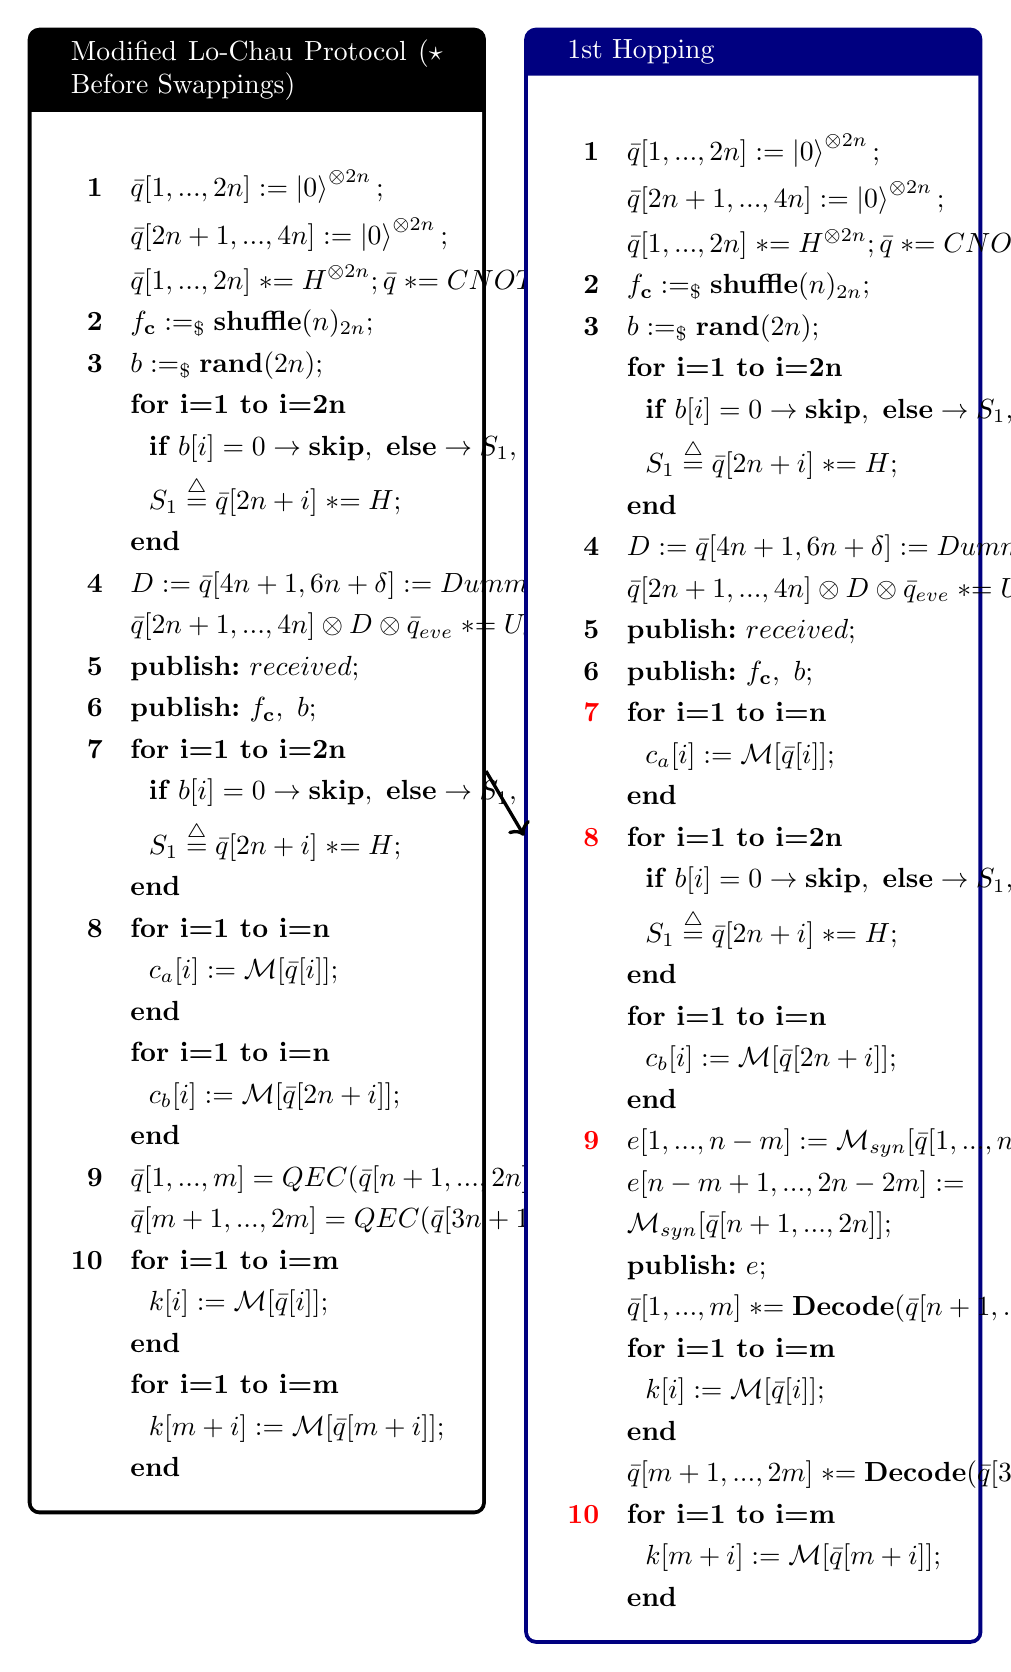
\begin{tikzpicture}[remember picture]
% Left box
\node[anchor=north west,inner sep=0pt,outer sep=0pt] (leftbox) at (0,0) {
\begin{minipage}[t]{0.48\textwidth}
\begin{tcolorbox}[colframe=black!75!black, colback=white, title=Modified Lo-Chau Protocol ($\star$ Before Swappings), width=\textwidth]
\begin{align*}
    \textbf{1} \quad & \bar{q}[1,...,2n] := \ket{0}^{\otimes 2n}; \\
    &\bar{q}[2n+1,...,4n] := \ket{0}^{\otimes 2n};\\
    \quad &\bar{q}[1,...,2n] \asteq H^{\otimes 2n}; \bar{q} \asteq CNOT; \\
    \textbf{2} \quad & f_{\textbf{c}}:=_\$\textbf{shuffle}(n)_{2n}; \\
    \textbf{3} \quad & b :=_\$ \textbf{rand}(2n); \\
    &\textbf{for~i=1~to~i=2n}\\
    &~~ \textbf{if }  b[i] = 0 \rightarrow \textbf{skip},~\textbf{else}\rightarrow S_{1},\\
    &~~ S_{1}\stackrel{\triangle}{=}\bar{q}[2n+i] \asteq H ;\\
    &\textbf{end}\\
    \textbf{4} \quad & {D}:= \bar{q}[4n+1,6n+\delta]:=Dummy;\\
    &\bar{q}[2n+1,...,4n]\otimes {D} \otimes \bar{q}_{eve} \asteq U_{\textbf{c}}(f_{\textbf{c}}); \\
    \textbf{5} \quad & \textbf{publish:}~ received;\\
    \textbf{6} \quad & \textbf{publish:}~ f_{\textbf{c}},~b;\\
    \textbf{7} \quad & \textbf{for~i=1~to~i=2n}\\
    &~~ \textbf{if }  b[i] = 0 \rightarrow \textbf{skip},~\textbf{else}\rightarrow S_{1} ,\\
    &~~ S_{1}\stackrel{\triangle}{=}\bar{q}[2n+i] \asteq H ;\\
    &\textbf{end}\\
    \textbf{8} \quad & \textbf{for~i=1~to~i=n}\\
    &~~ c_a[i]:= \mathcal{M} [\bar{q}[i]];\\
    &\textbf{end}\\
    \quad & \textbf{for~i=1~to~i=n}\\
    &~~ c_b[i]:= \mathcal{M} [\bar{q}[2n+i]];\\
    &\textbf{end}\\
    \textbf{9} \quad & \bar{q}[1,...,m]=QEC(\bar{q}[n+1,...,2n])\\
    \quad & \bar{q}[m+1,...,2m]=QEC(\bar{q}[3n+1,...,4n])\\
    \textbf{10} \quad & \textbf{for~i=1~to~i=m}\\
    &~~ k[i]:= \mathcal{M} [\bar{q}[i]];\\
    &\textbf{end}\\
    & \textbf{for~i=1~to~i=m}\\
    &~~ k[m+i]:= \mathcal{M} [\bar{q}[m+i]];\\
    &\textbf{end}
\end{align*}
\end{tcolorbox}
\end{minipage}
};

% Right box
\node[anchor=north west,inner sep=0pt,outer sep=0pt] (rightbox) at (0.52\textwidth,0) {
\begin{minipage}[t]{0.48\textwidth}
\begin{tcolorbox}[colframe=blue!50!black, colback=white, title=1st Hopping, width=\textwidth]
\begin{align*}
    \textbf{1} \quad & \bar{q}[1,...,2n] := \ket{0}^{\otimes 2n}; \\
    &\bar{q}[2n+1,...,4n] := \ket{0}^{\otimes 2n};\\
    \quad &\bar{q}[1,...,2n] \asteq H^{\otimes 2n}; \bar{q} \asteq CNOT; \\
    \textbf{2} \quad & f_{\textbf{c}}:=_\$\textbf{shuffle}(n)_{2n}; \\
    \textbf{3} \quad & b :=_\$ \textbf{rand}(2n); \\
    &\textbf{for~i=1~to~i=2n}\\
    &~~ \textbf{if }  b[i] = 0 \rightarrow \textbf{skip},~\textbf{else}\rightarrow S_{1},\\
    &~~ S_{1}\stackrel{\triangle}{=}\bar{q}[2n+i] \asteq H ;\\
    &\textbf{end}\\
    \textbf{4} \quad & {D}:= \bar{q}[4n+1,6n+\delta]:=Dummy;\\
    &\bar{q}[2n+1,...,4n]\otimes {D} \otimes \bar{q}_{eve} \asteq U_{\textbf{c}}(f_{\textbf{c}}); \\
    \textbf{5} \quad & \textbf{publish:}~ received;\\
    \textbf{6} \quad & \textbf{publish:}~ f_{\textbf{c}},~b;\\
    \textbf{\textcolor{red}{7}} \quad & \textbf{for~i=1~to~i=n}\\
    &~~ c_a[i]:= \mathcal{M} [\bar{q}[i]];\\
    &\textbf{end}\\
    \textbf{\textcolor{red}{8}} \quad & \textbf{for~i=1~to~i=2n}\\
    &~~ \textbf{if }  b[i] = 0 \rightarrow \textbf{skip},~\textbf{else}\rightarrow S_{1} ,\\
    &~~ S_{1}\stackrel{\triangle}{=}\bar{q}[2n+i] \asteq H ;\\
    &\textbf{end}\\
    \quad & \textbf{for~i=1~to~i=n}\\
    &~~ c_b[i]:= \mathcal{M} [\bar{q}[2n+i]];\\
    &\textbf{end}\\
    \textbf{\textcolor{red}{9}} \quad 
    & e[1,...,n-m]:=\mathcal{M}_{syn} [\bar{q}[1,...,n]];\\
    & e[n-m+1,...,2n-2m]:=\\
    &\mathcal{M}_{syn} [\bar{q}[n+1,...,2n]];\\
    & \textbf{publish:}~ e;\\
    & \bar{q}[1,...,m]\asteq\textbf{Decode}(\bar{q}[n+1,...,2n])\\
    & \textbf{for~i=1~to~i=m}\\
    &~~ k[i]:= \mathcal{M} [\bar{q}[i]];\\
    &\textbf{end}\\
    \quad & \bar{q}[m+1,...,2m]\asteq\textbf{Decode}(\bar{q}[3n+1,...,4n])\\
    \textbf{\textcolor{red}{10}} \quad 
    & \textbf{for~i=1~to~i=m}\\
    &~~ k[m+i]:= \mathcal{M} [\bar{q}[m+i]];\\
    &\textbf{end}
\end{align*}
\end{tcolorbox}
\end{minipage}
};

% Draw arrow between boxes
\draw[->, very thick] (leftbox.east) -- node[above]{} (rightbox.west);

\end{tikzpicture}
\newpage

\noindent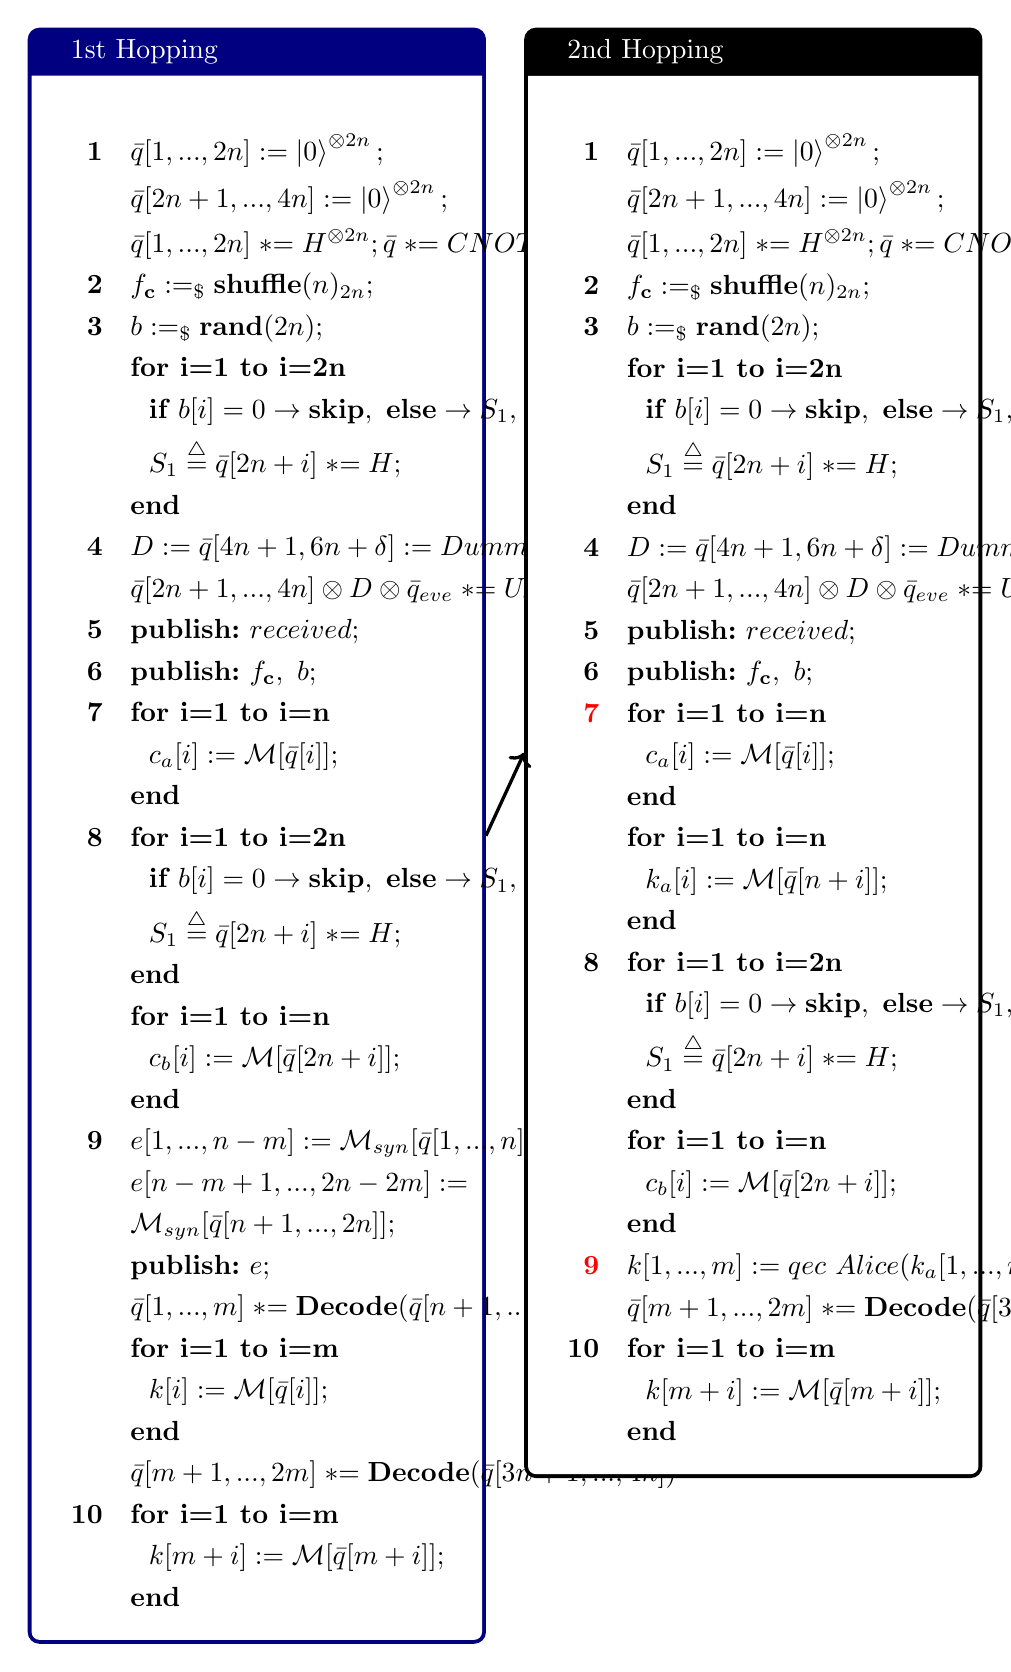
\begin{tikzpicture}[remember picture]

% Left box
\node[anchor=north west,inner sep=0pt,outer sep=0pt] (leftbox) at (0,0) {
\begin{minipage}[t]{0.48\textwidth}
\begin{tcolorbox}[colframe=blue!50!black, colback=white, title=1st Hopping , width=\textwidth]
\begin{align*}
    \textbf{1} \quad & \bar{q}[1,...,2n] := \ket{0}^{\otimes 2n}; \\
    &\bar{q}[2n+1,...,4n] := \ket{0}^{\otimes 2n};\\
    \quad &\bar{q}[1,...,2n] \asteq H^{\otimes 2n}; \bar{q} \asteq CNOT; \\
    \textbf{2} \quad & f_{\textbf{c}}:=_\$\textbf{shuffle}(n)_{2n}; \\
    \textbf{3} \quad & b :=_\$ \textbf{rand}(2n); \\
    &\textbf{for~i=1~to~i=2n}\\
    &~~ \textbf{if }  b[i] = 0 \rightarrow \textbf{skip},~\textbf{else}\rightarrow S_{1},\\
    &~~ S_{1}\stackrel{\triangle}{=}\bar{q}[2n+i] \asteq H ;\\
    &\textbf{end}\\
    \textbf{4} \quad & {D}:= \bar{q}[4n+1,6n+\delta]:=Dummy;\\
    &\bar{q}[2n+1,...,4n]\otimes {D} \otimes \bar{q}_{eve} \asteq U_{\textbf{c}}(f_{\textbf{c}}); \\
    \textbf{5} \quad & \textbf{publish:}~ received;\\
    \textbf{6} \quad & \textbf{publish:}~ f_{\textbf{c}},~b;\\
    \textbf{{7}} \quad & \textbf{for~i=1~to~i=n}\\
    &~~ c_a[i]:= \mathcal{M} [\bar{q}[i]];\\
    &\textbf{end}\\
    \textbf{{8}} \quad & \textbf{for~i=1~to~i=2n}\\
    &~~ \textbf{if }  b[i] = 0 \rightarrow \textbf{skip},~\textbf{else}\rightarrow S_{1} ,\\
    &~~ S_{1}\stackrel{\triangle}{=}\bar{q}[2n+i] \asteq H ;\\
    &\textbf{end}\\
    \quad & \textbf{for~i=1~to~i=n}\\
    &~~ c_b[i]:= \mathcal{M} [\bar{q}[2n+i]];\\
    &\textbf{end}\\
    \textbf{{9}} \quad 
    & e[1,...,n-m]:=\mathcal{M}_{syn} [\bar{q}[1,...,n]];\\
    & e[n-m+1,...,2n-2m]:=\\
    &\mathcal{M}_{syn} [\bar{q}[n+1,...,2n]];\\
    & \textbf{publish:}~ e;\\
    & \bar{q}[1,...,m]\asteq\textbf{Decode}(\bar{q}[n+1,...,2n])\\
    & \textbf{for~i=1~to~i=m}\\
    &~~ k[i]:= \mathcal{M} [\bar{q}[i]];\\
    &\textbf{end}\\
    \quad & \bar{q}[m+1,...,2m]\asteq\textbf{Decode}(\bar{q}[3n+1,...,4n])\\
    \textbf{{10}} \quad 
    & \textbf{for~i=1~to~i=m}\\
    &~~ k[m+i]:= \mathcal{M} [\bar{q}[m+i]];\\
    &\textbf{end}
\end{align*}
\end{tcolorbox}
\end{minipage}
};

% Right box
\node[anchor=north west,inner sep=0pt,outer sep=0pt] (rightbox) at (0.52\textwidth,0) {
\begin{minipage}[t]{0.48\textwidth}
\begin{tcolorbox}[colframe=black!50!black, colback=white, title=2nd Hopping, width=\textwidth]
\begin{align*}
    \textbf{1} \quad & \bar{q}[1,...,2n] := \ket{0}^{\otimes 2n}; \\
    &\bar{q}[2n+1,...,4n] := \ket{0}^{\otimes 2n};\\
    \quad &\bar{q}[1,...,2n] \asteq H^{\otimes 2n}; \bar{q} \asteq CNOT; \\
    \textbf{2} \quad & f_{\textbf{c}}:=_\$\textbf{shuffle}(n)_{2n}; \\
    \textbf{3} \quad & b :=_\$ \textbf{rand}(2n); \\
    &\textbf{for~i=1~to~i=2n}\\
    &~~ \textbf{if }  b[i] = 0 \rightarrow \textbf{skip},~\textbf{else}\rightarrow S_{1},\\
    &~~ S_{1}\stackrel{\triangle}{=}\bar{q}[2n+i] \asteq H ;\\
    &\textbf{end}\\
    \textbf{4} \quad & {D}:= \bar{q}[4n+1,6n+\delta]:=Dummy;\\
    &\bar{q}[2n+1,...,4n]\otimes {D} \otimes \bar{q}_{eve} \asteq U_{\textbf{c}}(f_{\textbf{c}}); \\
    \textbf{5} \quad & \textbf{publish:}~ received;\\
    \textbf{6} \quad & \textbf{publish:}~ f_{\textbf{c}},~b;\\
    \textbf{\textcolor{red}{7}} \quad & \textbf{for~i=1~to~i=n}\\
    &~~ c_a[i]:= \mathcal{M} [\bar{q}[i]];\\
    &\textbf{end}\\
    & \textbf{for~i=1~to~i=n}\\
    &~~ k_a[i]:= \mathcal{M} [\bar{q}[n+i]];\\
    &\textbf{end}\\
    \textbf{{8}} \quad & \textbf{for~i=1~to~i=2n}\\
    &~~ \textbf{if }  b[i] = 0 \rightarrow \textbf{skip},~\textbf{else}\rightarrow S_{1} ,\\
    &~~ S_{1}\stackrel{\triangle}{=}\bar{q}[2n+i] \asteq H ;\\
    &\textbf{end}\\
    \quad & \textbf{for~i=1~to~i=n}\\
    &~~ c_b[i]:= \mathcal{M} [\bar{q}[2n+i]];\\
    &\textbf{end}\\
    \textbf{\textcolor{red}{9}} \quad 
    & k[1,...,m]:=qec~Alice(k_a[1,...,n])\\
    \quad & \bar{q}[m+1,...,2m]\asteq\textbf{Decode}(\bar{q}[3n+1,...,4n])\\
    \textbf{{10}} \quad 
    & \textbf{for~i=1~to~i=m}\\
    &~~ k[m+i]:= \mathcal{M} [\bar{q}[m+i]];\\
    &\textbf{end}
\end{align*}
\end{tcolorbox}
\end{minipage}
};

% Draw arrow between boxes
\draw[->, very thick] (leftbox.east) -- node[above]{} (rightbox.west);

\end{tikzpicture}
\newpage



\noindent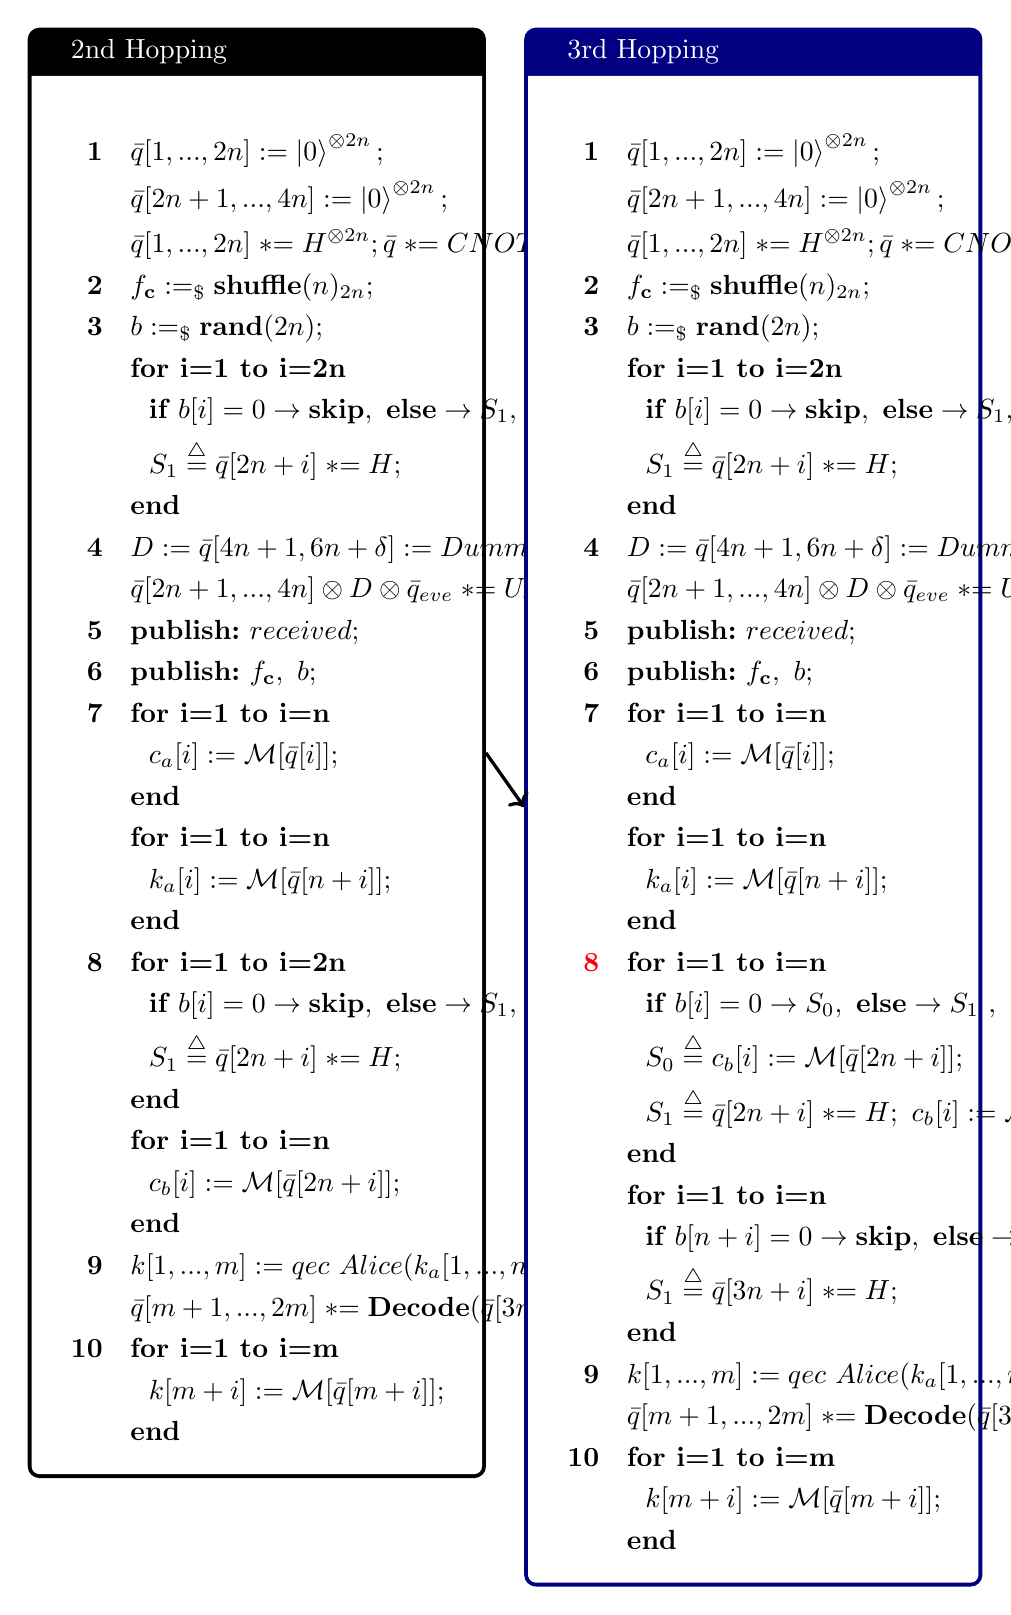
\begin{tikzpicture}[remember picture]

% Left box
\node[anchor=north west,inner sep=0pt,outer sep=0pt] (leftbox) at (0,0) {
\begin{minipage}[t]{0.48\textwidth}
\begin{tcolorbox}[colframe=black!75!black, colback=white, title=2nd Hopping, width=\textwidth]
\begin{align*}
    \textbf{1} \quad & \bar{q}[1,...,2n] := \ket{0}^{\otimes 2n}; \\
    &\bar{q}[2n+1,...,4n] := \ket{0}^{\otimes 2n};\\
    \quad &\bar{q}[1,...,2n] \asteq H^{\otimes 2n}; \bar{q} \asteq CNOT; \\
    \textbf{2} \quad & f_{\textbf{c}}:=_\$\textbf{shuffle}(n)_{2n}; \\
    \textbf{3} \quad & b :=_\$ \textbf{rand}(2n); \\
    &\textbf{for~i=1~to~i=2n}\\
    &~~ \textbf{if }  b[i] = 0 \rightarrow \textbf{skip},~\textbf{else}\rightarrow S_{1},\\
    &~~ S_{1}\stackrel{\triangle}{=}\bar{q}[2n+i] \asteq H ;\\
    &\textbf{end}\\
    \textbf{4} \quad & {D}:= \bar{q}[4n+1,6n+\delta]:=Dummy;\\
    &\bar{q}[2n+1,...,4n]\otimes {D} \otimes \bar{q}_{eve} \asteq U_{\textbf{c}}(f_{\textbf{c}}); \\
    \textbf{5} \quad & \textbf{publish:}~ received;\\
    \textbf{6} \quad & \textbf{publish:}~ f_{\textbf{c}},~b;\\
    \textbf{{7}} \quad & \textbf{for~i=1~to~i=n}\\
    &~~ c_a[i]:= \mathcal{M} [\bar{q}[i]];\\
    &\textbf{end}\\
    & \textbf{for~i=1~to~i=n}\\
    &~~ k_a[i]:= \mathcal{M} [\bar{q}[n+i]];\\
    &\textbf{end}\\
    \textbf{{8}} \quad & \textbf{for~i=1~to~i=2n}\\
    &~~ \textbf{if }  b[i] = 0 \rightarrow \textbf{skip},~\textbf{else}\rightarrow S_{1} ,\\
    &~~ S_{1}\stackrel{\triangle}{=}\bar{q}[2n+i] \asteq H ;\\
    &\textbf{end}\\
    \quad & \textbf{for~i=1~to~i=n}\\
    &~~ c_b[i]:= \mathcal{M} [\bar{q}[2n+i]];\\
    &\textbf{end}\\
    \textbf{{9}} \quad & k[1,...,m]:=qec~Alice(k_a[1,...,n])\\
    \quad & \bar{q}[m+1,...,2m]\asteq\textbf{Decode}(\bar{q}[3n+1,...,4n])\\
    \textbf{{10}} \quad 
    & \textbf{for~i=1~to~i=m}\\
    &~~ k[m+i]:= \mathcal{M} [\bar{q}[m+i]];\\
    &\textbf{end}
\end{align*}
\end{tcolorbox}
\end{minipage}
};

% Right box
\node[anchor=north west,inner sep=0pt,outer sep=0pt] (rightbox) at (0.52\textwidth,0) {
\begin{minipage}[t]{0.48\textwidth}
\begin{tcolorbox}[colframe=blue!50!black, colback=white, title=3rd Hopping, width=\textwidth]
\begin{align*}
    \textbf{1} \quad & \bar{q}[1,...,2n] := \ket{0}^{\otimes 2n}; \\
    &\bar{q}[2n+1,...,4n] := \ket{0}^{\otimes 2n};\\
    \quad &\bar{q}[1,...,2n] \asteq H^{\otimes 2n}; \bar{q} \asteq CNOT; \\
    \textbf{2} \quad & f_{\textbf{c}}:=_\$\textbf{shuffle}(n)_{2n}; \\
    \textbf{3} \quad & b :=_\$ \textbf{rand}(2n); \\
    &\textbf{for~i=1~to~i=2n}\\
    &~~ \textbf{if }  b[i] = 0 \rightarrow \textbf{skip},~\textbf{else}\rightarrow S_{1},\\
    &~~ S_{1}\stackrel{\triangle}{=}\bar{q}[2n+i] \asteq H ;\\
    &\textbf{end}\\
    \textbf{4} \quad & {D}:= \bar{q}[4n+1,6n+\delta]:=Dummy;\\
    &\bar{q}[2n+1,...,4n]\otimes {D} \otimes \bar{q}_{eve} \asteq U_{\textbf{c}}(f_{\textbf{c}}); \\
    \textbf{5} \quad & \textbf{publish:}~ received;\\
    \textbf{6} \quad & \textbf{publish:}~ f_{\textbf{c}},~b;\\
    \textbf{{7}} \quad & \textbf{for~i=1~to~i=n}\\
    &~~ c_a[i]:= \mathcal{M} [\bar{q}[i]];\\
    &\textbf{end}\\
    & \textbf{for~i=1~to~i=n}\\
    &~~ k_a[i]:= \mathcal{M} [\bar{q}[n+i]];\\
    &\textbf{end}\\
    \textbf{\textcolor{red}{8}} 
    \quad 
    &\textbf{for~i=1~to~i=n}\\
    &~~ \textbf{if }  b[i] = 0 \rightarrow S_{0},~\textbf{else}\rightarrow S_{1}~,\\
    &~~ S_{0}\stackrel{\triangle}{=}c_b[i]:= \mathcal{M}[\bar{q}[2n+i]];\\
    &~~ S_{1}\stackrel{\triangle}{=}\bar{q}[2n+i]\asteq H;~c_b[i]:= \mathcal{M}[\bar{q}[2n+i]];\\
    &\textbf{end}\\\quad 
    &\textbf{for~i=1~to~i=n}\\
    &~~ \textbf{if }  b[n+i] = 0 \rightarrow \textbf{skip},~\textbf{else}\rightarrow S_{1} ,\\
    &~~ S_{1}\stackrel{\triangle}{=}\bar{q}[3n+i] \asteq H ;\\
    &\textbf{end}\\
    \textbf{{9}} \quad & k[1,...,m]:=qec~Alice(k_a[1,...,n])\\
    \quad & \bar{q}[m+1,...,2m]\asteq\textbf{Decode}(\bar{q}[3n+1,...,4n])\\
    \textbf{{10}} \quad 
    & \textbf{for~i=1~to~i=m}\\
    &~~ k[m+i]:= \mathcal{M} [\bar{q}[m+i]];\\
    &\textbf{end}
\end{align*}
\end{tcolorbox}
\end{minipage}
};

% Draw arrow between boxes
\draw[->, very thick] (leftbox.east) -- node[above]{} (rightbox.west);

\end{tikzpicture}
\newpage

    
\noindent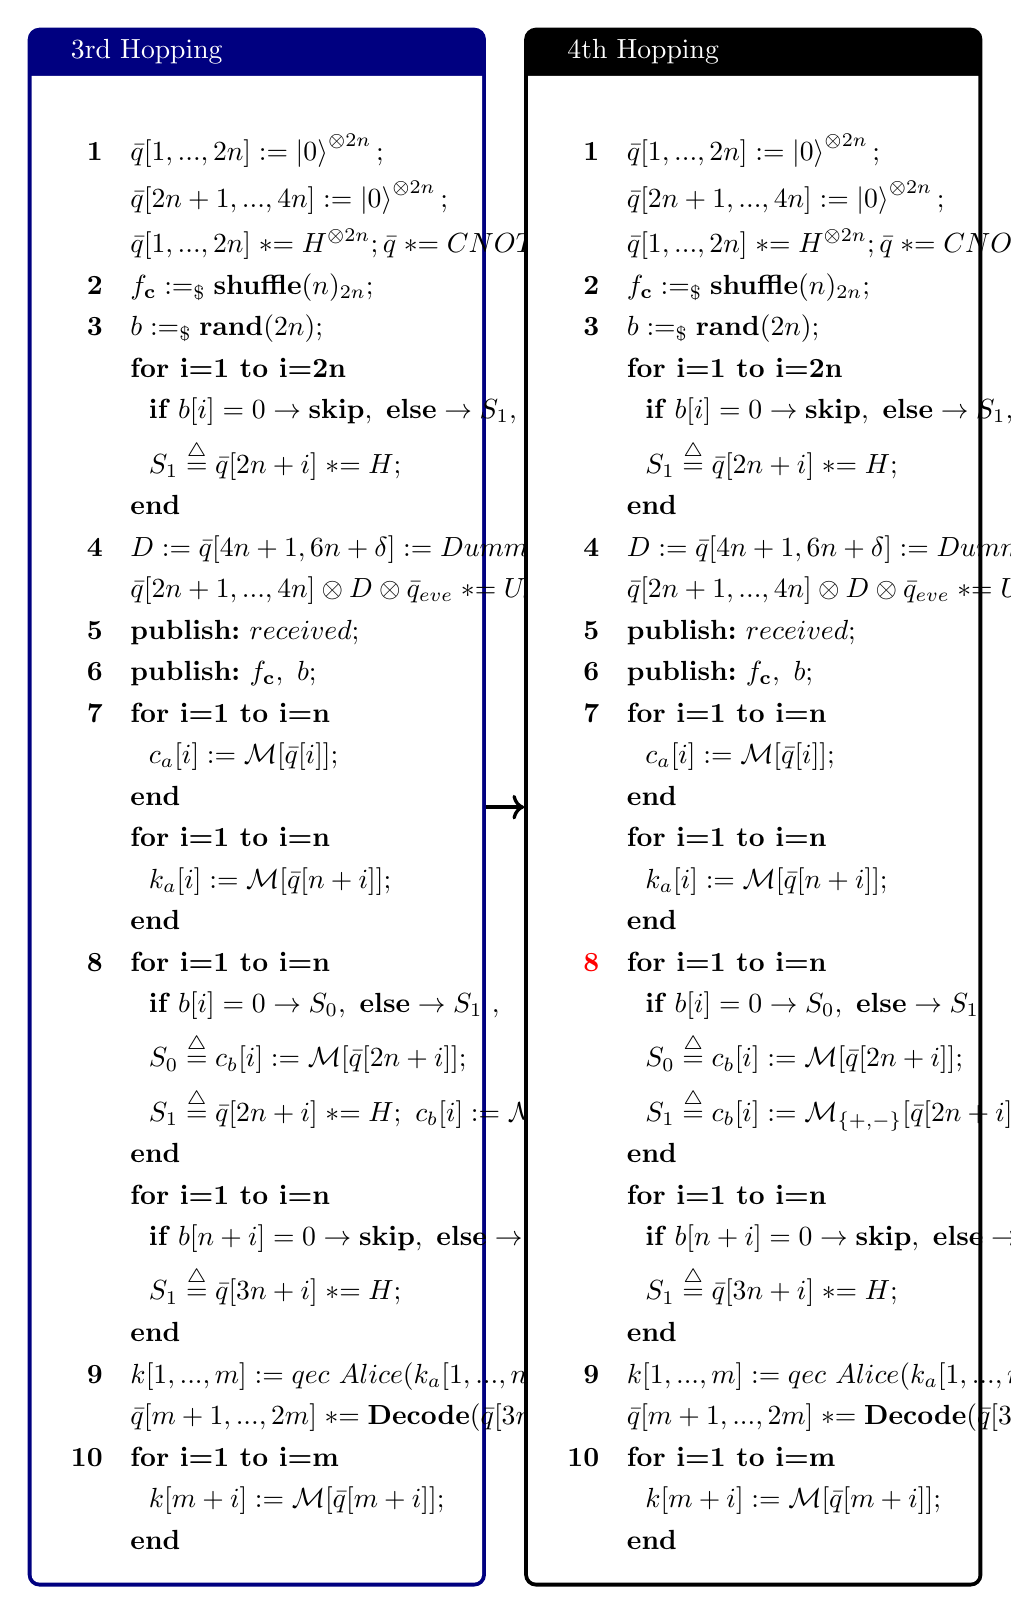
\begin{tikzpicture}[remember picture]

% Left box
\node[anchor=north west,inner sep=0pt,outer sep=0pt] (leftbox) at (0,0) {
\begin{minipage}[t]{0.48\textwidth}
\begin{tcolorbox}[colframe=blue!50!black, colback=white, title=3rd Hopping, width=\textwidth]
\begin{align*}
    \textbf{1} \quad & \bar{q}[1,...,2n] := \ket{0}^{\otimes 2n}; \\
    &\bar{q}[2n+1,...,4n] := \ket{0}^{\otimes 2n};\\
    \quad &\bar{q}[1,...,2n] \asteq H^{\otimes 2n}; \bar{q} \asteq CNOT; \\
    \textbf{2} \quad & f_{\textbf{c}}:=_\$\textbf{shuffle}(n)_{2n}; \\
    \textbf{3} \quad & b :=_\$ \textbf{rand}(2n); \\
    &\textbf{for~i=1~to~i=2n}\\
    &~~ \textbf{if }  b[i] = 0 \rightarrow \textbf{skip},~\textbf{else}\rightarrow S_{1},\\
    &~~ S_{1}\stackrel{\triangle}{=}\bar{q}[2n+i] \asteq H ;\\
    &\textbf{end}\\
    \textbf{4} \quad & {D}:= \bar{q}[4n+1,6n+\delta]:=Dummy;\\
    &\bar{q}[2n+1,...,4n]\otimes {D} \otimes \bar{q}_{eve} \asteq U_{\textbf{c}}(f_{\textbf{c}}); \\
    \textbf{5} \quad & \textbf{publish:}~ received;\\
    \textbf{6} \quad & \textbf{publish:}~ f_{\textbf{c}},~b;\\
    \textbf{{7}} \quad & \textbf{for~i=1~to~i=n}\\
    &~~ c_a[i]:= \mathcal{M} [\bar{q}[i]];\\
    &\textbf{end}\\
    & \textbf{for~i=1~to~i=n}\\
    &~~ k_a[i]:= \mathcal{M} [\bar{q}[n+i]];\\
    &\textbf{end}\\
    \textbf{{8}} 
    \quad 
    &\textbf{for~i=1~to~i=n}\\
    &~~ \textbf{if }  b[i] = 0 \rightarrow S_{0},~\textbf{else}\rightarrow S_{1}~,\\
    &~~ S_{0}\stackrel{\triangle}{=}c_b[i]:= \mathcal{M}[\bar{q}[2n+i]];\\
    &~~ S_{1}\stackrel{\triangle}{=}\bar{q}[2n+i]\asteq H;~c_b[i]:= \mathcal{M}[\bar{q}[2n+i]];\\
    &\textbf{end}\\\quad 
    &\textbf{for~i=1~to~i=n}\\
    &~~ \textbf{if }  b[n+i] = 0 \rightarrow \textbf{skip},~\textbf{else}\rightarrow S_{1} ,\\
    &~~ S_{1}\stackrel{\triangle}{=}\bar{q}[3n+i] \asteq H ;\\
    &\textbf{end}\\
    \textbf{{9}} \quad & k[1,...,m]:=qec~Alice(k_a[1,...,n])\\
    \quad & \bar{q}[m+1,...,2m]\asteq\textbf{Decode}(\bar{q}[3n+1,...,4n])\\
    \textbf{{10}} \quad 
    & \textbf{for~i=1~to~i=m}\\
    &~~ k[m+i]:= \mathcal{M} [\bar{q}[m+i]];\\
    &\textbf{end}
\end{align*}
\end{tcolorbox}
\end{minipage}
};

% Right box
\node[anchor=north west,inner sep=0pt,outer sep=0pt] (rightbox) at (0.52\textwidth,0) {
\begin{minipage}[t]{0.48\textwidth}
\begin{tcolorbox}[colframe=black!50!black, colback=white, title=4th Hopping, width=\textwidth]
\begin{align*}
    \textbf{1} \quad & \bar{q}[1,...,2n] := \ket{0}^{\otimes 2n}; \\
    &\bar{q}[2n+1,...,4n] := \ket{0}^{\otimes 2n};\\
    \quad &\bar{q}[1,...,2n] \asteq H^{\otimes 2n}; \bar{q} \asteq CNOT; \\
    \textbf{2} \quad & f_{\textbf{c}}:=_\$\textbf{shuffle}(n)_{2n}; \\
    \textbf{3} \quad & b :=_\$ \textbf{rand}(2n); \\
    &\textbf{for~i=1~to~i=2n}\\
    &~~ \textbf{if }  b[i] = 0 \rightarrow \textbf{skip},~\textbf{else}\rightarrow S_{1},\\
    &~~ S_{1}\stackrel{\triangle}{=}\bar{q}[2n+i] \asteq H ;\\
    &\textbf{end}\\
    \textbf{4} \quad & {D}:= \bar{q}[4n+1,6n+\delta]:=Dummy;\\
    &\bar{q}[2n+1,...,4n]\otimes {D} \otimes \bar{q}_{eve} \asteq U_{\textbf{c}}(f_{\textbf{c}}); \\
    \textbf{5} \quad & \textbf{publish:}~ received;\\
    \textbf{6} \quad & \textbf{publish:}~ f_{\textbf{c}},~b;\\
    \textbf{{7}} \quad & \textbf{for~i=1~to~i=n}\\
    &~~ c_a[i]:= \mathcal{M} [\bar{q}[i]];\\
    &\textbf{end}\\
    & \textbf{for~i=1~to~i=n}\\
    &~~ k_a[i]:= \mathcal{M} [\bar{q}[n+i]];\\
    &\textbf{end}\\
    \textbf{\textcolor{red}{8}} 
    \quad 
    &\textbf{for~i=1~to~i=n}\\
    &~~ \textbf{if }  b[i] = 0 \rightarrow S_{0},~\textbf{else}\rightarrow S_{1}\\
    &~~ S_{0}\stackrel{\triangle}{=}c_b[i]:= \mathcal{M} [\bar{q}[2n+i]];\\
    &~~ S_{1}\stackrel{\triangle}{=}c_b[i]:= \mathcal{M}_{\{+,-\}} [\bar{q}[2n+i]];\\
    &\textbf{end}\\
    &\textbf{for~i=1~to~i=n}\\
    &~~ \textbf{if }  b[n+i] = 0 \rightarrow \textbf{skip},~\textbf{else}\rightarrow S_{1} ,\\
    &~~ S_{1}\stackrel{\triangle}{=}\bar{q}[3n+i] \asteq H ;\\
    &\textbf{end}\\
    \textbf{{9}} \quad & k[1,...,m]:=qec~Alice(k_a[1,...,n])\\
    \quad & \bar{q}[m+1,...,2m]\asteq\textbf{Decode}(\bar{q}[3n+1,...,4n])\\
    \textbf{{10}} \quad 
    & \textbf{for~i=1~to~i=m}\\
    &~~ k[m+i]:= \mathcal{M} [\bar{q}[m+i]];\\
    &\textbf{end}
\end{align*}
\end{tcolorbox}
\end{minipage}
};

% Draw arrow between boxes
\draw[->, very thick] (leftbox.east) -- node[above]{} (rightbox.west);

\end{tikzpicture}
\newpage

\noindent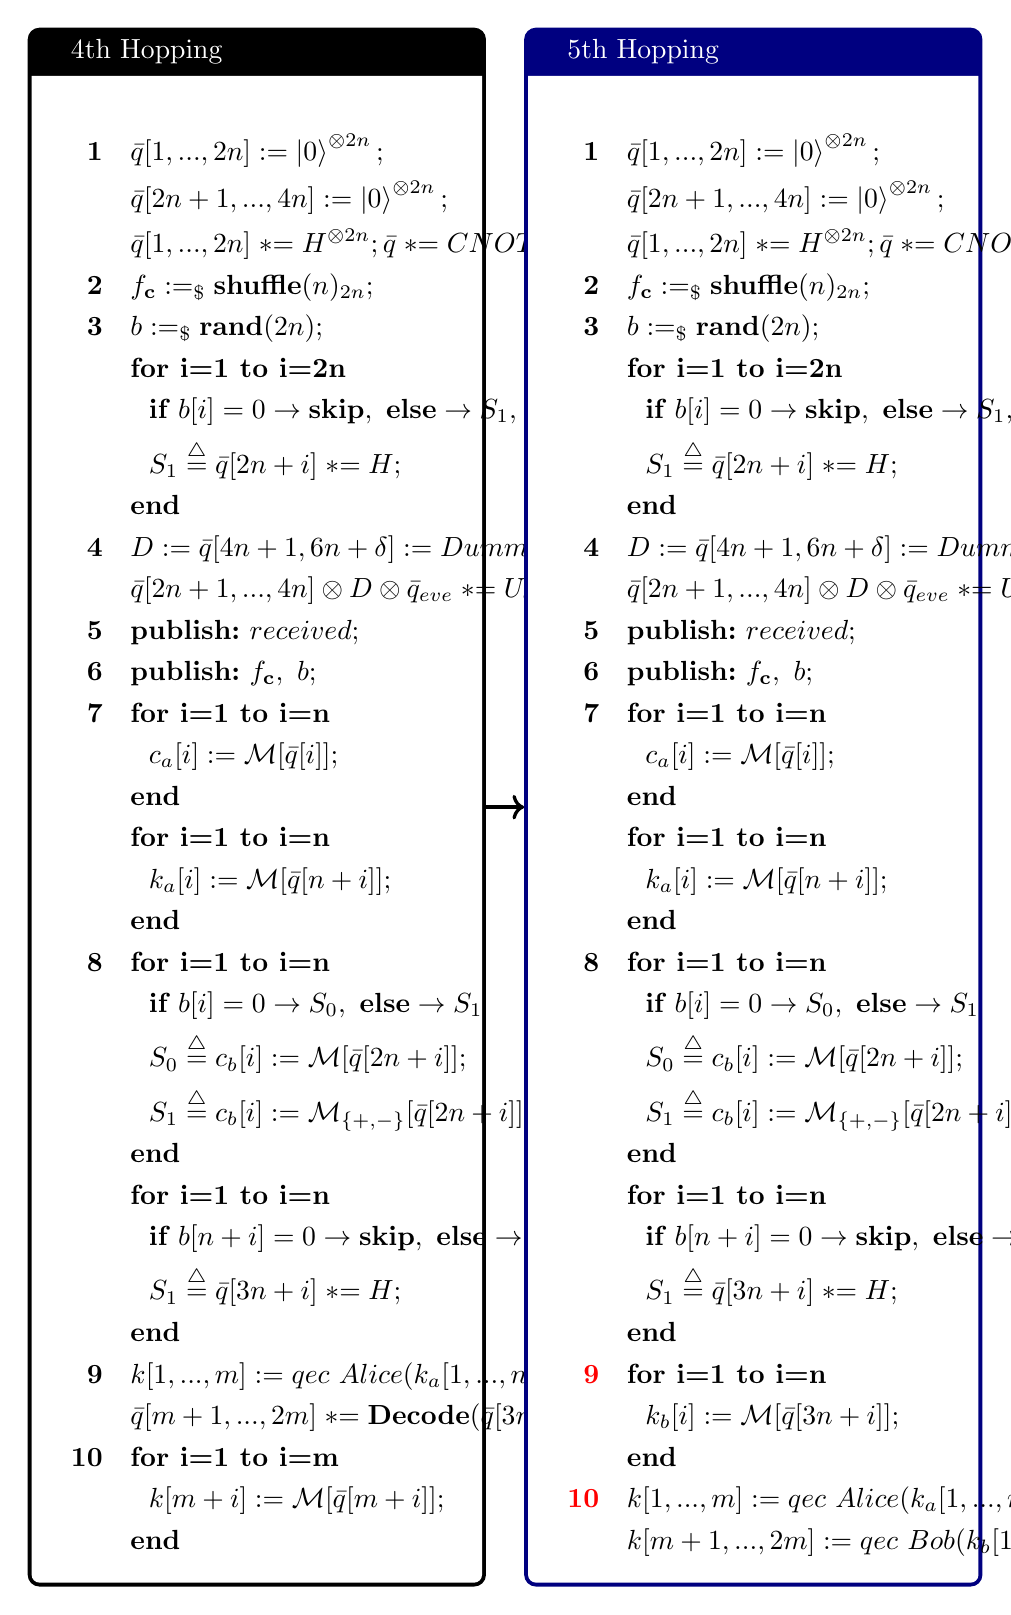
\begin{tikzpicture}[remember picture]

% Left box
\node[anchor=north west,inner sep=0pt,outer sep=0pt] (leftbox) at (0,0) {
\begin{minipage}[t]{0.48\textwidth}
\begin{tcolorbox}[colframe=black!50!black, colback=white, title=4th Hopping, width=\textwidth]
\begin{align*}
    \textbf{1} \quad & \bar{q}[1,...,2n] := \ket{0}^{\otimes 2n}; \\
    &\bar{q}[2n+1,...,4n] := \ket{0}^{\otimes 2n};\\
    \quad &\bar{q}[1,...,2n] \asteq H^{\otimes 2n}; \bar{q} \asteq CNOT; \\
    \textbf{2} \quad & f_{\textbf{c}}:=_\$\textbf{shuffle}(n)_{2n}; \\
    \textbf{3} \quad & b :=_\$ \textbf{rand}(2n); \\
    &\textbf{for~i=1~to~i=2n}\\
    &~~ \textbf{if }  b[i] = 0 \rightarrow \textbf{skip},~\textbf{else}\rightarrow S_{1},\\
    &~~ S_{1}\stackrel{\triangle}{=}\bar{q}[2n+i] \asteq H ;\\
    &\textbf{end}\\
    \textbf{4} \quad & {D}:= \bar{q}[4n+1,6n+\delta]:=Dummy;\\
    &\bar{q}[2n+1,...,4n]\otimes {D} \otimes \bar{q}_{eve} \asteq U_{\textbf{c}}(f_{\textbf{c}}); \\
    \textbf{5} \quad & \textbf{publish:}~ received;\\
    \textbf{6} \quad & \textbf{publish:}~ f_{\textbf{c}},~b;\\
    \textbf{{7}} \quad & \textbf{for~i=1~to~i=n}\\
    &~~ c_a[i]:= \mathcal{M} [\bar{q}[i]];\\
    &\textbf{end}\\
    & \textbf{for~i=1~to~i=n}\\
    &~~ k_a[i]:= \mathcal{M} [\bar{q}[n+i]];\\
    &\textbf{end}\\
    \textbf{{8}} 
    \quad 
    &\textbf{for~i=1~to~i=n}\\
    &~~ \textbf{if }  b[i] = 0 \rightarrow S_{0},~\textbf{else}\rightarrow S_{1}\\
    &~~ S_{0}\stackrel{\triangle}{=}c_b[i]:= \mathcal{M} [\bar{q}[2n+i]];\\
    &~~ S_{1}\stackrel{\triangle}{=}c_b[i]:= \mathcal{M}_{\{+,-\}} [\bar{q}[2n+i]];\\
    &\textbf{end}\\
    &\textbf{for~i=1~to~i=n}\\
    &~~ \textbf{if }  b[n+i] = 0 \rightarrow \textbf{skip},~\textbf{else}\rightarrow S_{1} ,\\
    &~~ S_{1}\stackrel{\triangle}{=}\bar{q}[3n+i] \asteq H ;\\
    &\textbf{end}\\
    \textbf{{9}} \quad & k[1,...,m]:=qec~Alice(k_a[1,...,n])\\
    \quad & \bar{q}[m+1,...,2m]\asteq\textbf{Decode}(\bar{q}[3n+1,...,4n])\\
    \textbf{{10}} \quad 
    & \textbf{for~i=1~to~i=m}\\
    &~~ k[m+i]:= \mathcal{M} [\bar{q}[m+i]];\\
    &\textbf{end}
\end{align*}
\end{tcolorbox}
\end{minipage}
};

% Right box
\node[anchor=north west,inner sep=0pt,outer sep=0pt] (rightbox) at (0.52\textwidth,0) {
\begin{minipage}[t]{0.48\textwidth}
\begin{tcolorbox}[colframe=blue!50!black, colback=white, title=5th Hopping, width=\textwidth]
\begin{align*}
    \textbf{1} \quad & \bar{q}[1,...,2n] := \ket{0}^{\otimes 2n}; \\
    &\bar{q}[2n+1,...,4n] := \ket{0}^{\otimes 2n};\\
    \quad &\bar{q}[1,...,2n] \asteq H^{\otimes 2n}; \bar{q} \asteq CNOT; \\
    \textbf{2} \quad & f_{\textbf{c}}:=_\$\textbf{shuffle}(n)_{2n}; \\
    \textbf{3} \quad & b :=_\$ \textbf{rand}(2n); \\
    &\textbf{for~i=1~to~i=2n}\\
    &~~ \textbf{if }  b[i] = 0 \rightarrow \textbf{skip},~\textbf{else}\rightarrow S_{1},\\
    &~~ S_{1}\stackrel{\triangle}{=}\bar{q}[2n+i] \asteq H ;\\
    &\textbf{end}\\
    \textbf{4} \quad & {D}:= \bar{q}[4n+1,6n+\delta]:=Dummy;\\
    &\bar{q}[2n+1,...,4n]\otimes {D} \otimes \bar{q}_{eve} \asteq U_{\textbf{c}}(f_{\textbf{c}}); \\
    \textbf{5} \quad & \textbf{publish:}~ received;\\
    \textbf{6} \quad & \textbf{publish:}~ f_{\textbf{c}},~b;\\
    \textbf{{7}} \quad & \textbf{for~i=1~to~i=n}\\
    &~~ c_a[i]:= \mathcal{M} [\bar{q}[i]];\\
    &\textbf{end}\\
    & \textbf{for~i=1~to~i=n}\\
    &~~ k_a[i]:= \mathcal{M} [\bar{q}[n+i]];\\
    &\textbf{end}\\
    \textbf{{8}} 
    \quad 
    &\textbf{for~i=1~to~i=n}\\
    &~~ \textbf{if }  b[i] = 0 \rightarrow S_{0},~\textbf{else}\rightarrow S_{1}\\
    &~~ S_{0}\stackrel{\triangle}{=}c_b[i]:= \mathcal{M} [\bar{q}[2n+i]];\\
    &~~ S_{1}\stackrel{\triangle}{=}c_b[i]:= \mathcal{M}_{\{+,-\}} [\bar{q}[2n+i]];\\
    &\textbf{end}\\
    &\textbf{for~i=1~to~i=n}\\
    &~~ \textbf{if }  b[n+i] = 0 \rightarrow \textbf{skip},~\textbf{else}\rightarrow S_{1} ,\\
    &~~ S_{1}\stackrel{\triangle}{=}\bar{q}[3n+i] \asteq H ;\\
    &\textbf{end}\\
    \textbf{\textcolor{red}{9}} \quad & \textbf{for~i=1~to~i=n}\\
    &~~ k_b[i]:= \mathcal{M} [\bar{q}[3n+i]];\\
    &\textbf{end}\\
    \textbf{\textcolor{red}{10}} \quad & k[1,...,m]:=qec~Alice(k_a[1,...,n])\\
    \quad & k[m+1,...,2m]:=qec~Bob(k_b[1,...,n])
\end{align*}
\end{tcolorbox}
\end{minipage}
};

% Draw arrow between boxes
\draw[->, very thick] (leftbox.east) -- node[above]{} (rightbox.west);

\end{tikzpicture}
\newpage


\noindent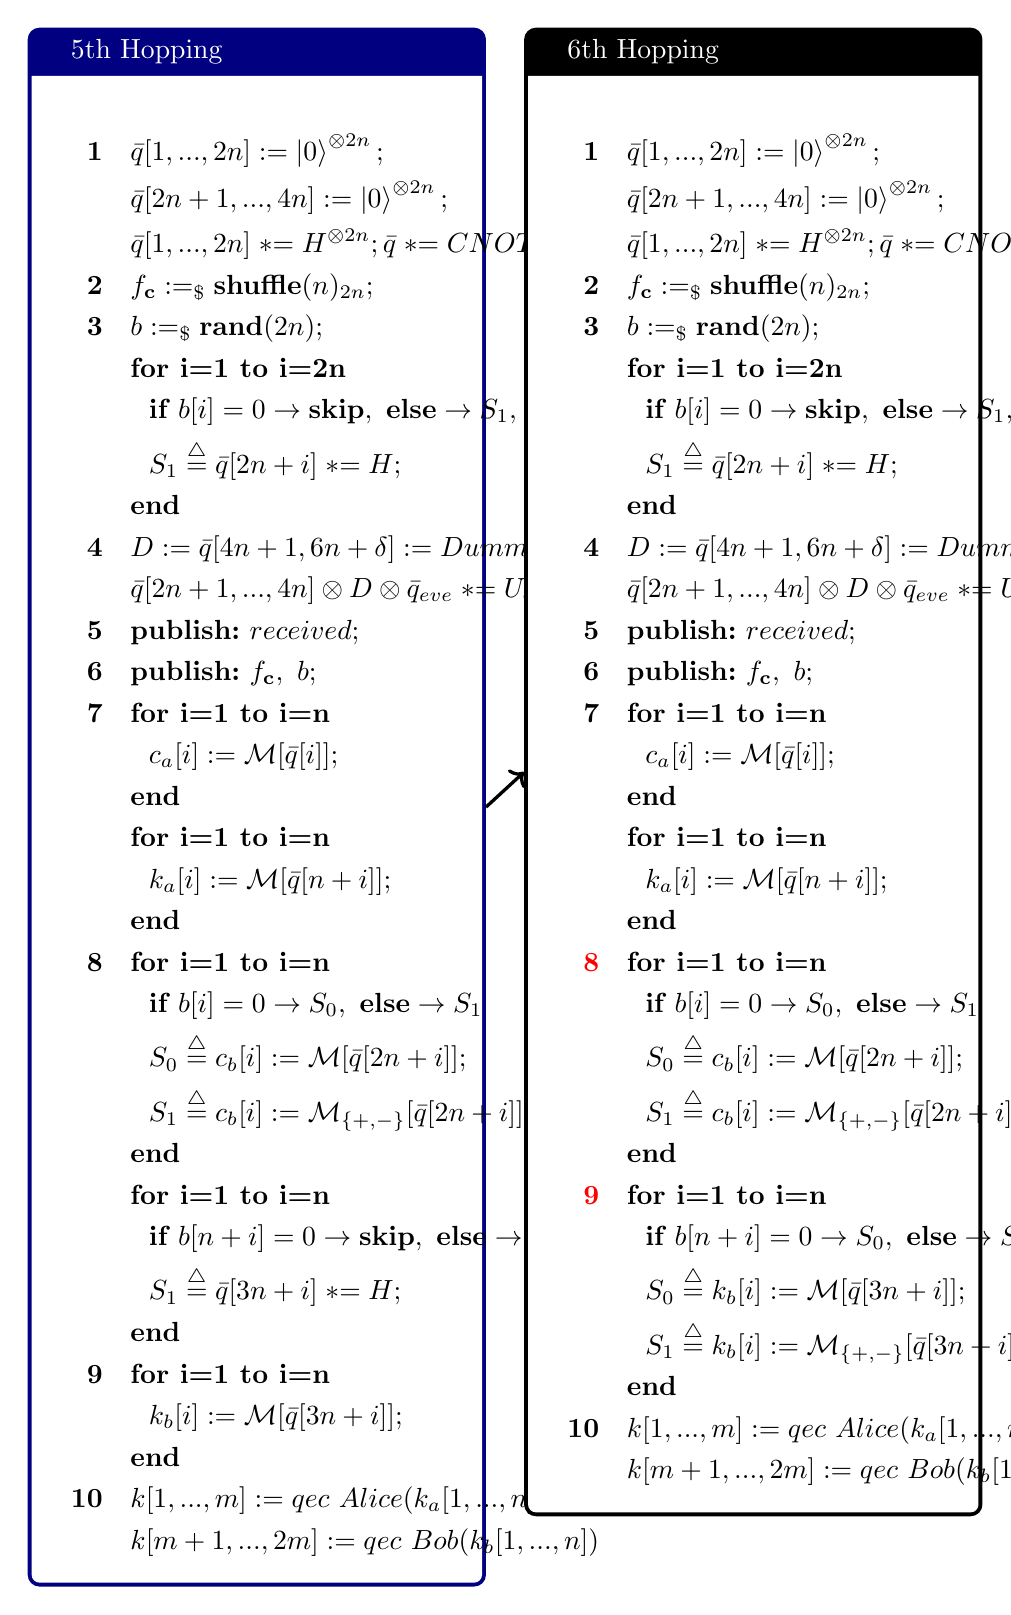
\begin{tikzpicture}[remember picture]

% Left box
\node[anchor=north west,inner sep=0pt,outer sep=0pt] (leftbox) at (0,0) {
\begin{minipage}[t]{0.48\textwidth}
\begin{tcolorbox}[colframe=blue!50!black, colback=white, title=5th Hopping, width=\textwidth]
\begin{align*}
    \textbf{1} \quad & \bar{q}[1,...,2n] := \ket{0}^{\otimes 2n}; \\
    &\bar{q}[2n+1,...,4n] := \ket{0}^{\otimes 2n};\\
    \quad &\bar{q}[1,...,2n] \asteq H^{\otimes 2n}; \bar{q} \asteq CNOT; \\
    \textbf{2} \quad & f_{\textbf{c}}:=_\$\textbf{shuffle}(n)_{2n}; \\
    \textbf{3} \quad & b :=_\$ \textbf{rand}(2n); \\
    &\textbf{for~i=1~to~i=2n}\\
    &~~ \textbf{if }  b[i] = 0 \rightarrow \textbf{skip},~\textbf{else}\rightarrow S_{1},\\
    &~~ S_{1}\stackrel{\triangle}{=}\bar{q}[2n+i] \asteq H ;\\
    &\textbf{end}\\
    \textbf{4} \quad & {D}:= \bar{q}[4n+1,6n+\delta]:=Dummy;\\
    &\bar{q}[2n+1,...,4n]\otimes {D} \otimes \bar{q}_{eve} \asteq U_{\textbf{c}}(f_{\textbf{c}}); \\
    \textbf{5} \quad & \textbf{publish:}~ received;\\
    \textbf{6} \quad & \textbf{publish:}~ f_{\textbf{c}},~b;\\
    \textbf{{7}} \quad & \textbf{for~i=1~to~i=n}\\
    &~~ c_a[i]:= \mathcal{M} [\bar{q}[i]];\\
    &\textbf{end}\\
    & \textbf{for~i=1~to~i=n}\\
    &~~ k_a[i]:= \mathcal{M} [\bar{q}[n+i]];\\
    &\textbf{end}\\
    \textbf{{8}} 
    \quad 
    &\textbf{for~i=1~to~i=n}\\
    &~~ \textbf{if }  b[i] = 0 \rightarrow S_{0},~\textbf{else}\rightarrow S_{1}\\
    &~~ S_{0}\stackrel{\triangle}{=}c_b[i]:= \mathcal{M} [\bar{q}[2n+i]];\\
    &~~ S_{1}\stackrel{\triangle}{=}c_b[i]:= \mathcal{M}_{\{+,-\}} [\bar{q}[2n+i]];\\
    &\textbf{end}\\
    &\textbf{for~i=1~to~i=n}\\
    &~~ \textbf{if }  b[n+i] = 0 \rightarrow \textbf{skip},~\textbf{else}\rightarrow S_{1} ,\\
    &~~ S_{1}\stackrel{\triangle}{=}\bar{q}[3n+i] \asteq H ;\\
    &\textbf{end}\\
    \textbf{{9}} \quad & \textbf{for~i=1~to~i=n}\\
    &~~ k_b[i]:= \mathcal{M} [\bar{q}[3n+i]];\\
    &\textbf{end}\\
    \textbf{{10}} \quad & k[1,...,m]:=qec~Alice(k_a[1,...,n])\\
    \quad & k[m+1,...,2m]:=qec~Bob(k_b[1,...,n])
\end{align*}
\end{tcolorbox}
\end{minipage}
};

% Right box
\node[anchor=north west,inner sep=0pt,outer sep=0pt] (rightbox) at (0.52\textwidth,0) {
\begin{minipage}[t]{0.48\textwidth}
\begin{tcolorbox}[colframe=black!50!black, colback=white, title=6th Hopping, width=\textwidth]
\begin{align*}
    \textbf{1} \quad & \bar{q}[1,...,2n] := \ket{0}^{\otimes 2n}; \\
    &\bar{q}[2n+1,...,4n] := \ket{0}^{\otimes 2n};\\
    \quad &\bar{q}[1,...,2n] \asteq H^{\otimes 2n}; \bar{q} \asteq CNOT; \\
    \textbf{2} \quad & f_{\textbf{c}}:=_\$\textbf{shuffle}(n)_{2n}; \\
    \textbf{3} \quad & b :=_\$ \textbf{rand}(2n); \\
    &\textbf{for~i=1~to~i=2n}\\
    &~~ \textbf{if }  b[i] = 0 \rightarrow \textbf{skip},~\textbf{else}\rightarrow S_{1},\\
    &~~ S_{1}\stackrel{\triangle}{=}\bar{q}[2n+i] \asteq H ;\\
    &\textbf{end}\\
    \textbf{4} \quad & {D}:= \bar{q}[4n+1,6n+\delta]:=Dummy;\\
    &\bar{q}[2n+1,...,4n]\otimes {D} \otimes \bar{q}_{eve} \asteq U_{\textbf{c}}(f_{\textbf{c}}); \\
    \textbf{5} \quad & \textbf{publish:}~ received;\\
    \textbf{6} \quad & \textbf{publish:}~ f_{\textbf{c}},~b;\\
    \textbf{{7}} \quad & \textbf{for~i=1~to~i=n}\\
    &~~ c_a[i]:= \mathcal{M} [\bar{q}[i]];\\
    &\textbf{end}\\
    & \textbf{for~i=1~to~i=n}\\
    &~~ k_a[i]:= \mathcal{M} [\bar{q}[n+i]];\\
    &\textbf{end}\\
    \textbf{\textcolor{red}{8}} 
    \quad 
    &\textbf{for~i=1~to~i=n}\\
    &~~ \textbf{if }  b[i] = 0 \rightarrow S_{0},~\textbf{else}\rightarrow S_{1}\\
    &~~ S_{0}\stackrel{\triangle}{=}c_b[i]:= \mathcal{M} [\bar{q}[2n+i]];\\
    &~~ S_{1}\stackrel{\triangle}{=}c_b[i]:= \mathcal{M}_{\{+,-\}} [\bar{q}[2n+i]];\\
    &\textbf{end}\\
    \textbf{\textcolor{red}{9}} \quad &\textbf{for~i=1~to~i=n}\\
    &~~ \textbf{if }  b[n+i] = 0 \rightarrow S_{0},~\textbf{else}\rightarrow S_{1}\\
    &~~ S_{0}\stackrel{\triangle}{=}k_b[i]:= \mathcal{M} [\bar{q}[3n+i]];\\
    &~~ S_{1}\stackrel{\triangle}{=}k_b[i]:= \mathcal{M}_{\{+,-\}} [\bar{q}[3n+i]];\\
    &\textbf{end}\\
    \textbf{{10}} \quad & k[1,...,m]:=qec~Alice(k_a[1,...,n])\\
    \quad & k[m+1,...,2m]:=qec~Bob(k_b[1,...,n])
\end{align*}
\end{tcolorbox}
\end{minipage}
};

% Draw arrow between boxes
\draw[->, very thick] (leftbox.east) -- node[above]{} (rightbox.west);

\end{tikzpicture}
\newpage

\noindent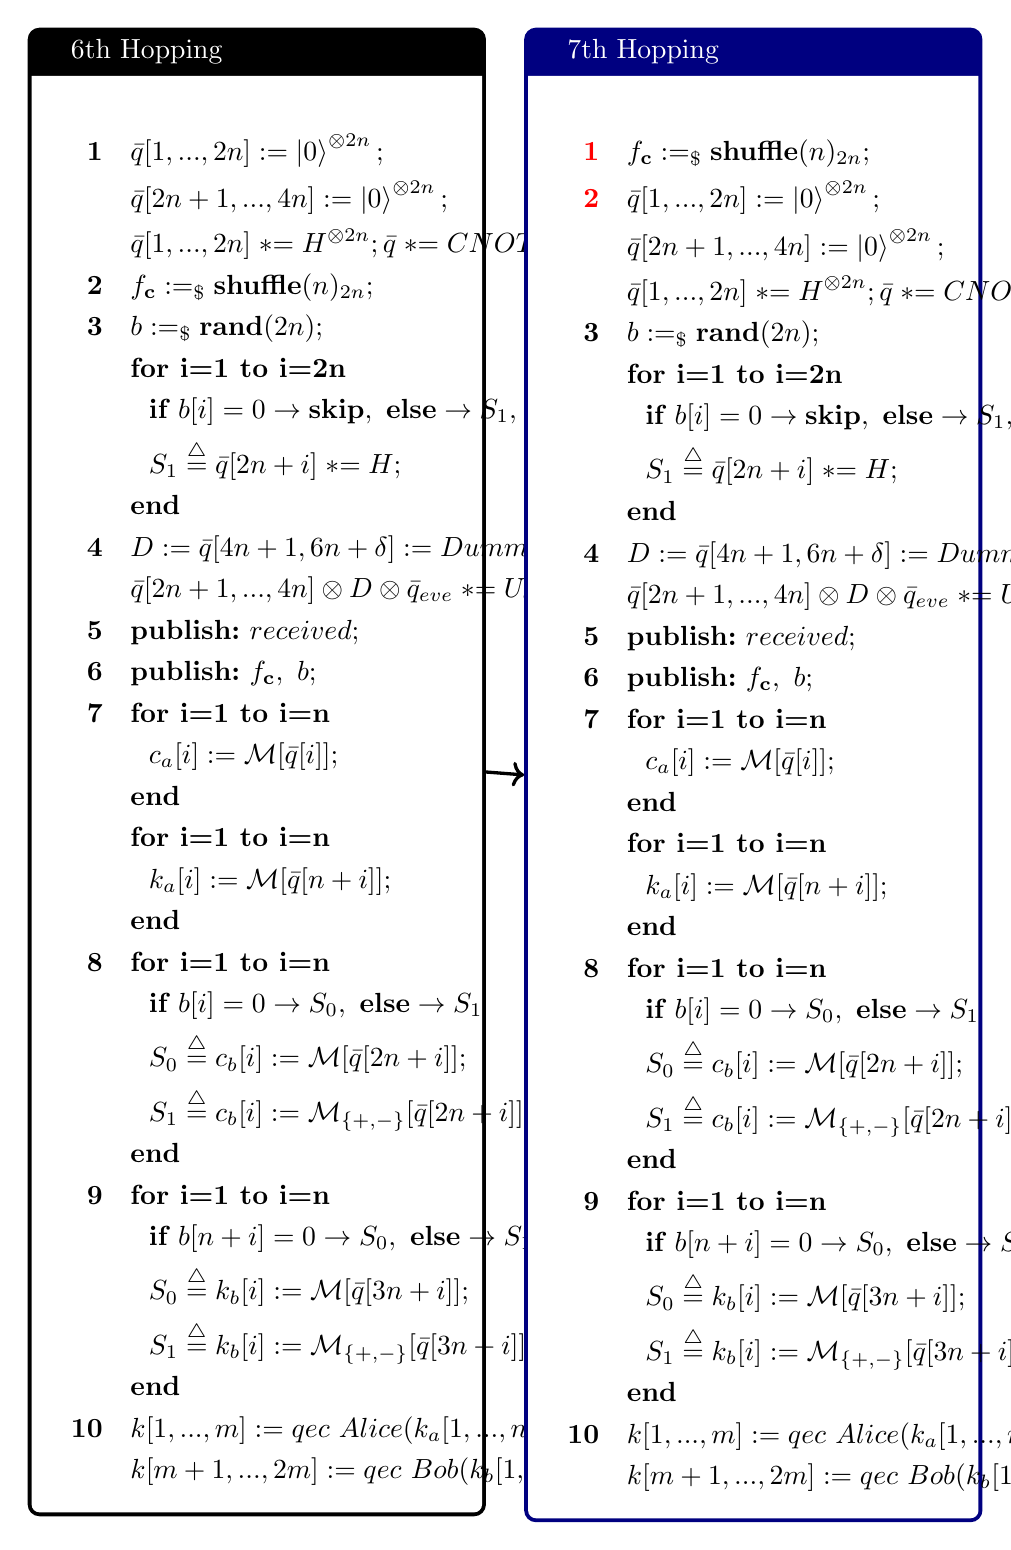
\begin{tikzpicture}[remember picture]

% Left box
\node[anchor=north west,inner sep=0pt,outer sep=0pt] (leftbox) at (0,0) {
\begin{minipage}[t]{0.48\textwidth}
\begin{tcolorbox}[colframe=black!50!black, colback=white, title=6th Hopping, width=\textwidth]
\begin{align*}
    \textbf{1} \quad & \bar{q}[1,...,2n] := \ket{0}^{\otimes 2n}; \\
    &\bar{q}[2n+1,...,4n] := \ket{0}^{\otimes 2n};\\
    \quad &\bar{q}[1,...,2n] \asteq H^{\otimes 2n}; \bar{q} \asteq CNOT; \\
    \textbf{2} \quad & f_{\textbf{c}}:=_\$\textbf{shuffle}(n)_{2n}; \\
    \textbf{3} \quad & b :=_\$ \textbf{rand}(2n); \\
    &\textbf{for~i=1~to~i=2n}\\
    &~~ \textbf{if }  b[i] = 0 \rightarrow \textbf{skip},~\textbf{else}\rightarrow S_{1},\\
    &~~ S_{1}\stackrel{\triangle}{=}\bar{q}[2n+i] \asteq H ;\\
    &\textbf{end}\\
    \textbf{4} \quad & {D}:= \bar{q}[4n+1,6n+\delta]:=Dummy;\\
    &\bar{q}[2n+1,...,4n]\otimes {D} \otimes \bar{q}_{eve} \asteq U_{\textbf{c}}(f_{\textbf{c}}); \\
    \textbf{5} \quad & \textbf{publish:}~ received;\\
    \textbf{6} \quad & \textbf{publish:}~ f_{\textbf{c}},~b;\\
    \textbf{{7}} \quad & \textbf{for~i=1~to~i=n}\\
    &~~ c_a[i]:= \mathcal{M} [\bar{q}[i]];\\
    &\textbf{end}\\
    & \textbf{for~i=1~to~i=n}\\
    &~~ k_a[i]:= \mathcal{M} [\bar{q}[n+i]];\\
    &\textbf{end}\\
    \textbf{{8}} 
    \quad 
    &\textbf{for~i=1~to~i=n}\\
    &~~ \textbf{if }  b[i] = 0 \rightarrow S_{0},~\textbf{else}\rightarrow S_{1}\\
    &~~ S_{0}\stackrel{\triangle}{=}c_b[i]:= \mathcal{M} [\bar{q}[2n+i]];\\
    &~~ S_{1}\stackrel{\triangle}{=}c_b[i]:= \mathcal{M}_{\{+,-\}} [\bar{q}[2n+i]];\\
    &\textbf{end}\\
    \textbf{{9}} \quad &\textbf{for~i=1~to~i=n}\\
    &~~ \textbf{if }  b[n+i] = 0 \rightarrow S_{0},~\textbf{else}\rightarrow S_{1}\\
    &~~ S_{0}\stackrel{\triangle}{=}k_b[i]:= \mathcal{M} [\bar{q}[3n+i]];\\
    &~~ S_{1}\stackrel{\triangle}{=}k_b[i]:= \mathcal{M}_{\{+,-\}} [\bar{q}[3n+i]];\\
    &\textbf{end}\\
    \textbf{{10}} \quad & k[1,...,m]:=qec~Alice(k_a[1,...,n])\\
    \quad & k[m+1,...,2m]:=qec~Bob(k_b[1,...,n])
\end{align*}
\end{tcolorbox}
\end{minipage}
};

% Right box
\node[anchor=north west,inner sep=0pt,outer sep=0pt] (rightbox) at (0.52\textwidth,0) {
\begin{minipage}[t]{0.48\textwidth}
\begin{tcolorbox}[colframe=blue!50!black, colback=white, title=7th Hopping, width=\textwidth]
\begin{align*}
    \textcolor{red}{\textbf{1}} \quad & f_{\textbf{c}}:=_\$\textbf{shuffle}(n)_{2n}; \\
    \textcolor{red}{\textbf{2}} \quad & \bar{q}[1,...,2n] := \ket{0}^{\otimes 2n}; \\
    &\bar{q}[2n+1,...,4n] := \ket{0}^{\otimes 2n};\\
    \quad &\bar{q}[1,...,2n] \asteq H^{\otimes 2n}; \bar{q} \asteq CNOT; \\
    \textbf{3} \quad & b :=_\$ \textbf{rand}(2n); \\
    &\textbf{for~i=1~to~i=2n}\\
    &~~ \textbf{if }  b[i] = 0 \rightarrow \textbf{skip},~\textbf{else}\rightarrow S_{1},\\
    &~~ S_{1}\stackrel{\triangle}{=}\bar{q}[2n+i] \asteq H ;\\
    &\textbf{end}\\
    \textbf{4} \quad & {D}:= \bar{q}[4n+1,6n+\delta]:=Dummy;\\
    &\bar{q}[2n+1,...,4n]\otimes {D} \otimes \bar{q}_{eve} \asteq U_{\textbf{c}}(f_{\textbf{c}}); \\
    \textbf{5} \quad & \textbf{publish:}~ received;\\
    \textbf{6} \quad & \textbf{publish:}~ f_{\textbf{c}},~b;\\
    \textbf{{7}} \quad & \textbf{for~i=1~to~i=n}\\
    &~~ c_a[i]:= \mathcal{M} [\bar{q}[i]];\\
    &\textbf{end}\\
    & \textbf{for~i=1~to~i=n}\\
    &~~ k_a[i]:= \mathcal{M} [\bar{q}[n+i]];\\
    &\textbf{end}\\
    \textbf{{8}} 
    \quad 
    &\textbf{for~i=1~to~i=n}\\
    &~~ \textbf{if }  b[i] = 0 \rightarrow S_{0},~\textbf{else}\rightarrow S_{1}\\
    &~~ S_{0}\stackrel{\triangle}{=}c_b[i]:= \mathcal{M} [\bar{q}[2n+i]];\\
    &~~ S_{1}\stackrel{\triangle}{=}c_b[i]:= \mathcal{M}_{\{+,-\}} [\bar{q}[2n+i]];\\
    &\textbf{end}\\
    \textbf{{9}} \quad &\textbf{for~i=1~to~i=n}\\
    &~~ \textbf{if }  b[n+i] = 0 \rightarrow S_{0},~\textbf{else}\rightarrow S_{1}\\
    &~~ S_{0}\stackrel{\triangle}{=}k_b[i]:= \mathcal{M} [\bar{q}[3n+i]];\\
    &~~ S_{1}\stackrel{\triangle}{=}k_b[i]:= \mathcal{M}_{\{+,-\}} [\bar{q}[3n+i]];\\
    &\textbf{end}\\
    \textbf{{10}} \quad & k[1,...,m]:=qec~Alice(k_a[1,...,n])\\
    \quad & k[m+1,...,2m]:=qec~Bob(k_b[1,...,n])
\end{align*}
\end{tcolorbox}
\end{minipage}
};

% Draw arrow between boxes
\draw[->, very thick] (leftbox.east) -- node[above]{} (rightbox.west);

\end{tikzpicture}
\newpage



\noindent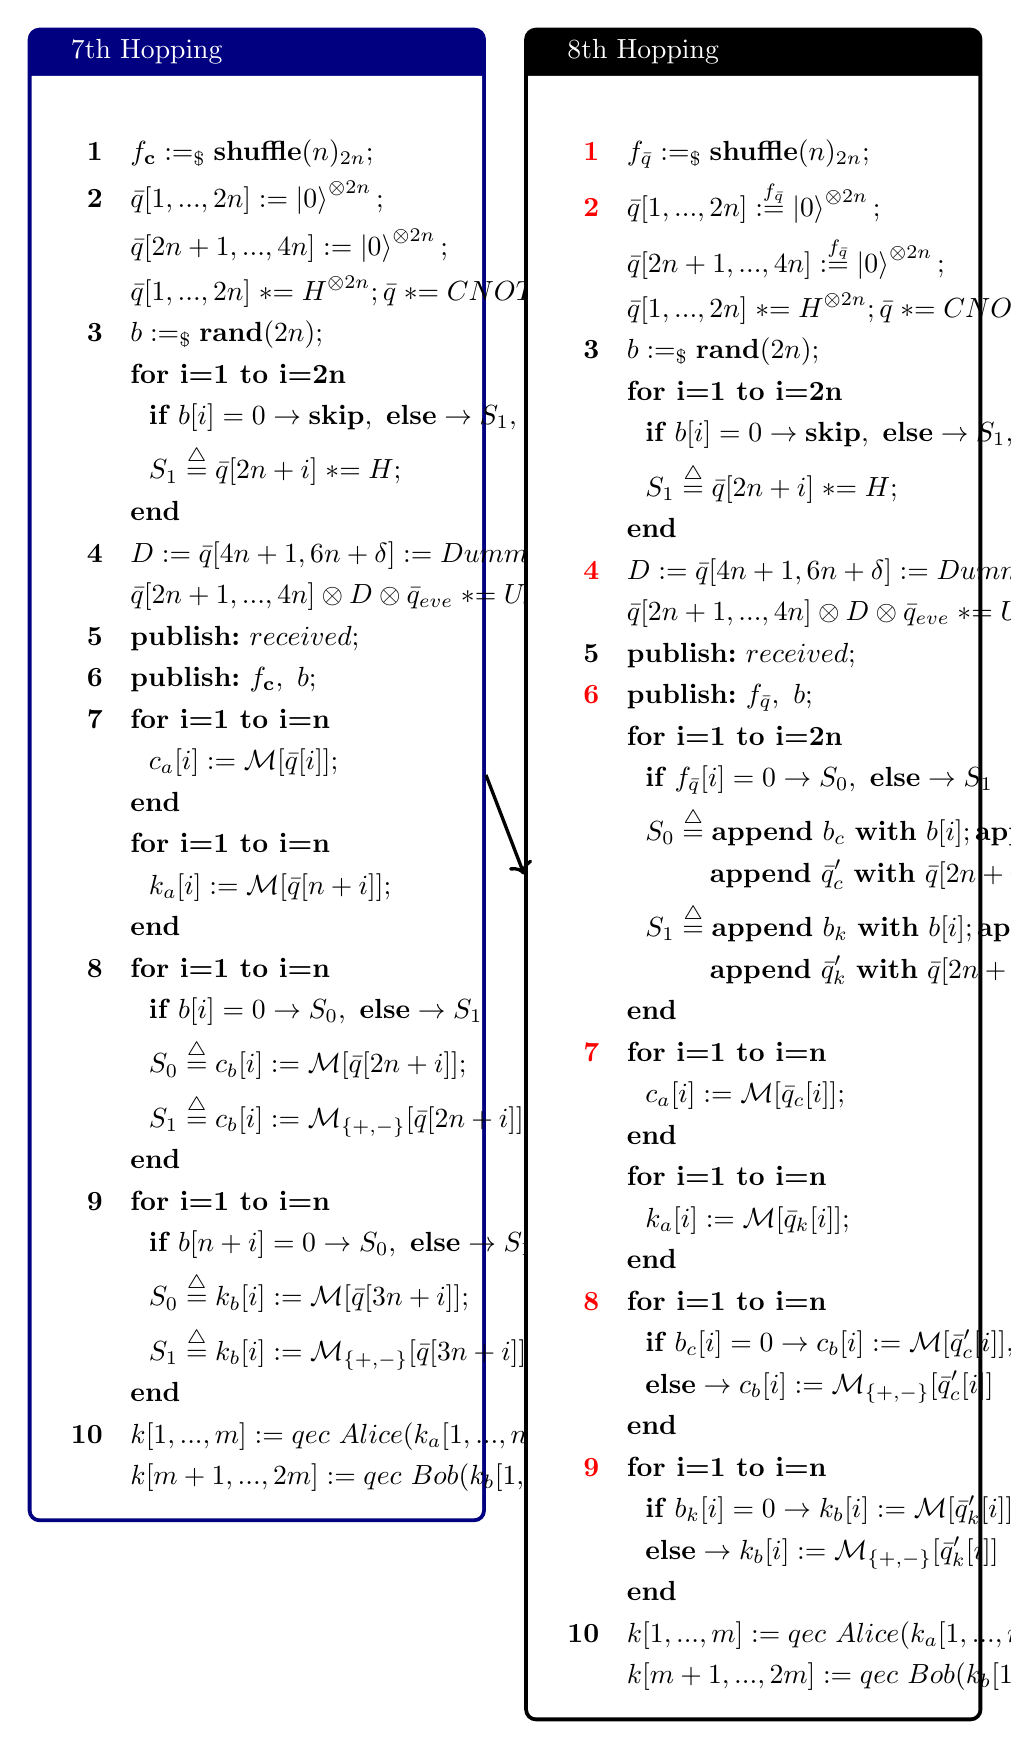
\begin{tikzpicture}[remember picture]

% Left box
\node[anchor=north west,inner sep=0pt,outer sep=0pt] (leftbox) at (0,0) {
\begin{minipage}[t]{0.48\textwidth}
\begin{tcolorbox}[colframe=blue!50!black, colback=white, title=7th Hopping, width=\textwidth]
\begin{align*}
    {\textbf{1}} \quad & f_{\textbf{c}}:=_\$\textbf{shuffle}(n)_{2n}; \\
    {\textbf{2}} \quad & \bar{q}[1,...,2n] := \ket{0}^{\otimes 2n}; \\
    &\bar{q}[2n+1,...,4n] := \ket{0}^{\otimes 2n};\\
    \quad &\bar{q}[1,...,2n] \asteq H^{\otimes 2n}; \bar{q} \asteq CNOT; \\
    \textbf{3} \quad & b :=_\$ \textbf{rand}(2n); \\
    &\textbf{for~i=1~to~i=2n}\\
    &~~ \textbf{if }  b[i] = 0 \rightarrow \textbf{skip},~\textbf{else}\rightarrow S_{1},\\
    &~~ S_{1}\stackrel{\triangle}{=}\bar{q}[2n+i] \asteq H ;\\
    &\textbf{end}\\
    \textbf{4} \quad & {D}:= \bar{q}[4n+1,6n+\delta]:=Dummy;\\
    &\bar{q}[2n+1,...,4n]\otimes {D} \otimes \bar{q}_{eve} \asteq U_{\textbf{c}}(f_{\textbf{c}}); \\
    \textbf{5} \quad & \textbf{publish:}~ received;\\
    \textbf{6} \quad & \textbf{publish:}~ f_{\textbf{c}},~b;\\
    \textbf{{7}} \quad & \textbf{for~i=1~to~i=n}\\
    &~~ c_a[i]:= \mathcal{M} [\bar{q}[i]];\\
    &\textbf{end}\\
    & \textbf{for~i=1~to~i=n}\\
    &~~ k_a[i]:= \mathcal{M} [\bar{q}[n+i]];\\
    &\textbf{end}\\
    \textbf{{8}} 
    \quad 
    &\textbf{for~i=1~to~i=n}\\
    &~~ \textbf{if }  b[i] = 0 \rightarrow S_{0},~\textbf{else}\rightarrow S_{1}\\
    &~~ S_{0}\stackrel{\triangle}{=}c_b[i]:= \mathcal{M} [\bar{q}[2n+i]];\\
    &~~ S_{1}\stackrel{\triangle}{=}c_b[i]:= \mathcal{M}_{\{+,-\}} [\bar{q}[2n+i]];\\
    &\textbf{end}\\
    \textbf{{9}} \quad &\textbf{for~i=1~to~i=n}\\
    &~~ \textbf{if }  b[n+i] = 0 \rightarrow S_{0},~\textbf{else}\rightarrow S_{1}\\
    &~~ S_{0}\stackrel{\triangle}{=}k_b[i]:= \mathcal{M} [\bar{q}[3n+i]];\\
    &~~ S_{1}\stackrel{\triangle}{=}k_b[i]:= \mathcal{M}_{\{+,-\}} [\bar{q}[3n+i]];\\
    &\textbf{end}\\
    \textbf{{10}} \quad & k[1,...,m]:=qec~Alice(k_a[1,...,n])\\
    \quad & k[m+1,...,2m]:=qec~Bob(k_b[1,...,n])
\end{align*}
\end{tcolorbox}
\end{minipage}
};

% Right box
\node[anchor=north west,inner sep=0pt,outer sep=0pt] (rightbox) at (0.52\textwidth,0) {
\begin{minipage}[t]{0.48\textwidth}
\begin{tcolorbox}[colframe=black!50!black, colback=white, title=8th Hopping, width=\textwidth]
\begin{align*}
    \textbf{\textcolor{red}{1}} \quad 
    & f_{\bar{q}}:=_\$\textbf{shuffle}(n)_{2n}; \\
    \textcolor{red}{\textbf{2}} \quad & \bar{q}[1,...,2n] :\stackrel{f_{\bar{q}}}{=} \ket{0}^{\otimes 2n}; \\
    &\bar{q}[2n+1,...,4n] :\stackrel{f_{\bar{q}}}{=} \ket{0}^{\otimes 2n};\\
    \quad &\bar{q}[1,...,2n] \asteq H^{\otimes 2n}; \bar{q} \asteq CNOT; \\
    \textbf{3} \quad & b :=_\$ \textbf{rand}(2n); \\
    &\textbf{for~i=1~to~i=2n}\\
    &~~ \textbf{if }  b[i] = 0 \rightarrow \textbf{skip},~\textbf{else}\rightarrow S_{1},\\
    &~~ S_{1}\stackrel{\triangle}{=}\bar{q}[2n+i] \asteq H ;\\
    &\textbf{end}\\
    \textcolor{red}{\textbf{4}} \quad & {D}:= \bar{q}[4n+1,6n+\delta]:=Dummy;\\
    &\bar{q}[2n+1,...,4n]\otimes {D} \otimes \bar{q}_{eve} \asteq U_{\textbf{channel}}; \\
    \textbf{5} \quad & \textbf{publish:}~ received;\\
    \textcolor{red}{\textbf{6}} \quad & \textbf{publish:}~ f_{\bar{q}},~b;\\
    &\textbf{for~i=1~to~i=2n}\\
    &~~ \textbf{if }  f_{\bar{q}}[i] = 0 \rightarrow S_{0},~\textbf{else}\rightarrow S_{1}\\
    &~~ S_{0}\stackrel{\triangle}{=}\textbf{append}~b_c~\textbf{with}~b[i];\textbf{append}~\bar{q}_c~\textbf{with}~\bar{q}[i];\\
    &~~~~~~~~~\textbf{append}~\bar{q}'_c~\textbf{with}~\bar{q}[2n+i];\\
    &~~ S_{1}\stackrel{\triangle}{=}\textbf{append}~b_k~\textbf{with}~b[i];\textbf{append}~\bar{q}_k~\textbf{with}~\bar{q}[i];\\
    &~~~~~~~~~\textbf{append}~\bar{q}'_k~\textbf{with}~\bar{q}[2n+i];\\
    &\textbf{end}\\
    \textcolor{red}{\textbf{{7}}} \quad & \textbf{for~i=1~to~i=n}\\
    &~~ c_a[i]:= \mathcal{M} [\bar{q}_{c}[i]];\\
    &\textbf{end}\\
    & \textbf{for~i=1~to~i=n}\\
    &~~ k_a[i]:= \mathcal{M} [\bar{q}_{k}[i]];\\
    &\textbf{end}\\
    \textcolor{red}{\textbf{{8}}} 
    \quad 
    &\textbf{for~i=1~to~i=n}\\
    &~~ \textbf{if }  b_c[i] = 0 \rightarrow c_b[i]:= \mathcal{M} [\bar{q}'_{c}[i]] ,\\
    &~~\textbf{else}\rightarrow c_b[i]:= \mathcal{M}_{\{+,-\}} [\bar{q}'_{c}[i]]\\
    &\textbf{end}\\
    \textcolor{red}{\textbf{{9}}} \quad &\textbf{for~i=1~to~i=n}\\
    &~~ \textbf{if }  b_k[i] = 0 \rightarrow k_b[i]:= \mathcal{M} [\bar{q}'_{k}[i]] ,\\
    &~~\textbf{else}\rightarrow k_b[i]:= \mathcal{M}_{\{+,-\}} [\bar{q}'_{k}[i]]\\
    &\textbf{end}\\
    \textbf{{10}} \quad & k[1,...,m]:=qec~Alice(k_a[1,...,n])\\
    \quad & k[m+1,...,2m]:=qec~Bob(k_b[1,...,n])
\end{align*}
\end{tcolorbox}
\end{minipage}
};

% Draw arrow between boxes
\draw[->, very thick] (leftbox.east) -- node[above]{} (rightbox.west);

\end{tikzpicture}
\newpage

\noindent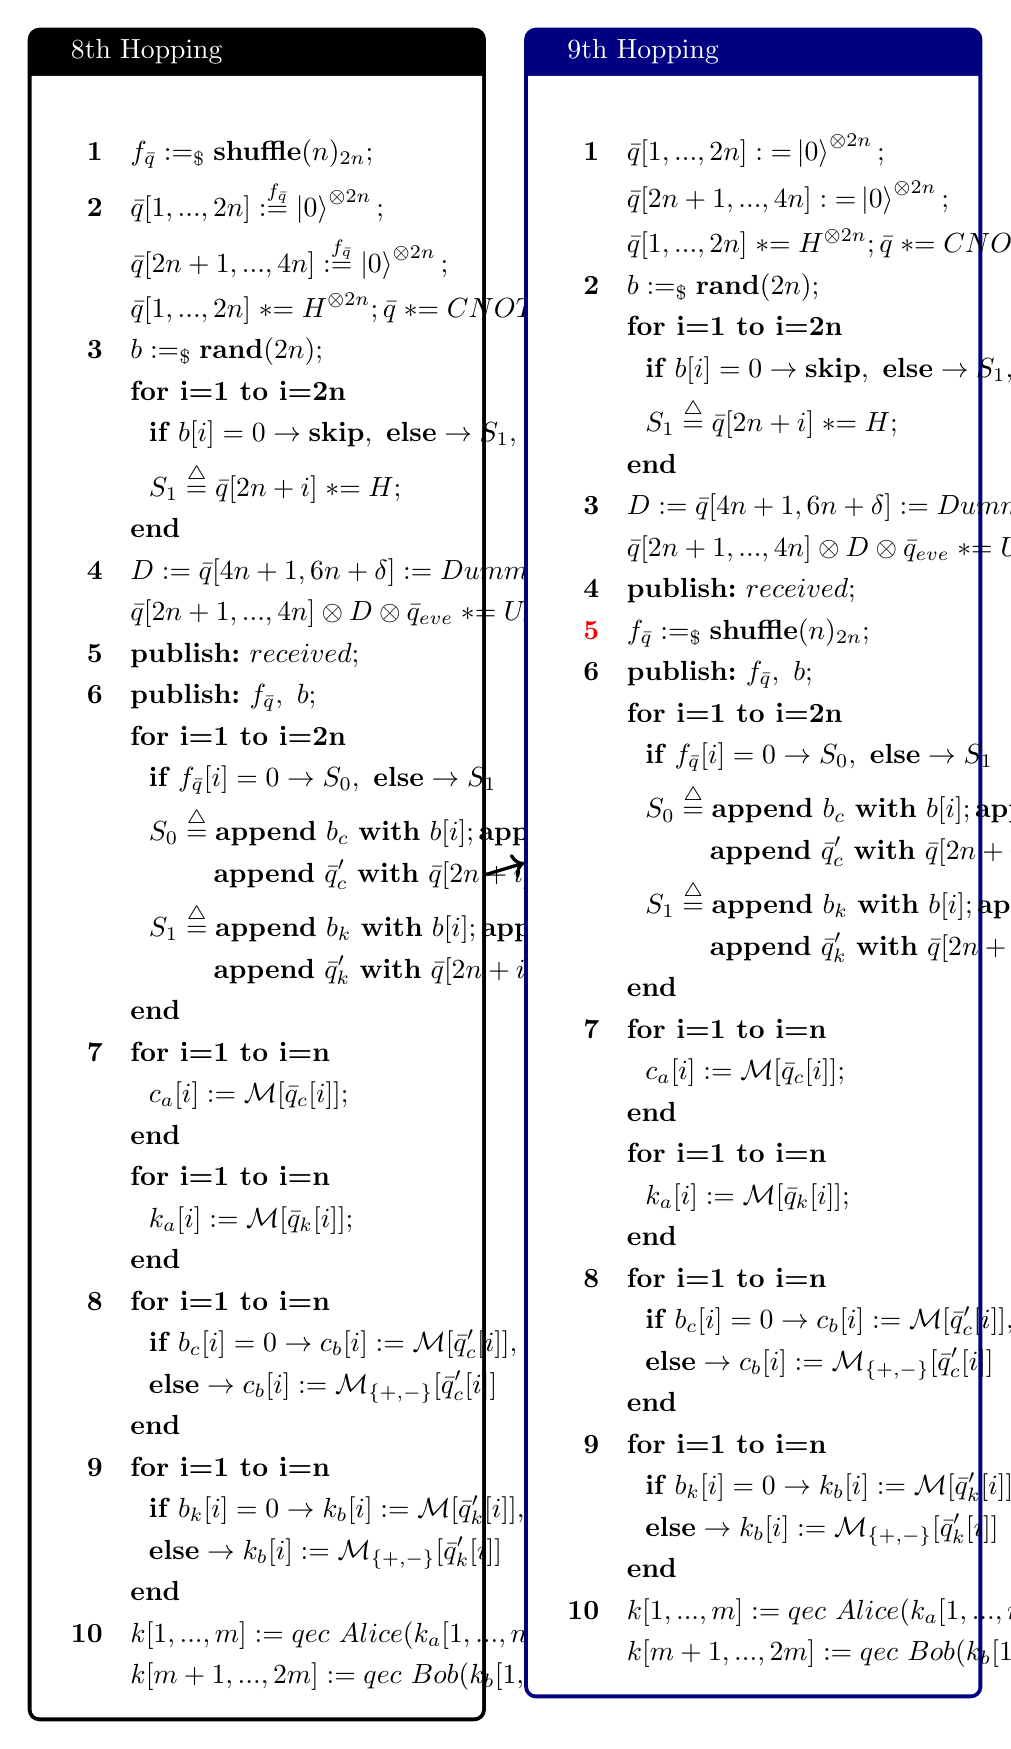
\begin{tikzpicture}[remember picture]

% Left box
\node[anchor=north west,inner sep=0pt,outer sep=0pt] (leftbox) at (0,0) {
\begin{minipage}[t]{0.48\textwidth}
\begin{tcolorbox}[colframe=black!50!black, colback=white, title=8th Hopping, width=\textwidth]
\begin{align*}
    \textbf{{1}} \quad 
    & f_{\bar{q}}:=_\$\textbf{shuffle}(n)_{2n}; \\
    {\textbf{2}} \quad & \bar{q}[1,...,2n] :\stackrel{f_{\bar{q}}}{=} \ket{0}^{\otimes 2n}; \\
    &\bar{q}[2n+1,...,4n] :\stackrel{f_{\bar{q}}}{=} \ket{0}^{\otimes 2n};\\
    \quad &\bar{q}[1,...,2n] \asteq H^{\otimes 2n}; \bar{q} \asteq CNOT; \\
    \textbf{3} \quad & b :=_\$ \textbf{rand}(2n); \\
    &\textbf{for~i=1~to~i=2n}\\
    &~~ \textbf{if }  b[i] = 0 \rightarrow \textbf{skip},~\textbf{else}\rightarrow S_{1},\\
    &~~ S_{1}\stackrel{\triangle}{=}\bar{q}[2n+i] \asteq H ;\\
    &\textbf{end}\\
    {\textbf{4}} \quad & {D}:= \bar{q}[4n+1,6n+\delta]:=Dummy;\\
    &\bar{q}[2n+1,...,4n]\otimes {D} \otimes \bar{q}_{eve} \asteq U_{\textbf{channel}}; \\
    \textbf{5} \quad & \textbf{publish:}~ received;\\
    {\textbf{6}} \quad & \textbf{publish:}~ f_{\bar{q}},~b;\\
    &\textbf{for~i=1~to~i=2n}\\
    &~~ \textbf{if }  f_{\bar{q}}[i] = 0 \rightarrow S_{0},~\textbf{else}\rightarrow S_{1}\\
    &~~ S_{0}\stackrel{\triangle}{=}\textbf{append}~b_c~\textbf{with}~b[i];\textbf{append}~\bar{q}_c~\textbf{with}~\bar{q}[i];\\
    &~~~~~~~~~\textbf{append}~\bar{q}'_c~\textbf{with}~\bar{q}[2n+i];\\
    &~~ S_{1}\stackrel{\triangle}{=}\textbf{append}~b_k~\textbf{with}~b[i];\textbf{append}~\bar{q}_k~\textbf{with}~\bar{q}[i];\\
    &~~~~~~~~~\textbf{append}~\bar{q}'_k~\textbf{with}~\bar{q}[2n+i];\\
    &\textbf{end}\\
    {\textbf{{7}}} \quad & \textbf{for~i=1~to~i=n}\\
    &~~ c_a[i]:= \mathcal{M} [\bar{q}_{c}[i]];\\
    &\textbf{end}\\
    & \textbf{for~i=1~to~i=n}\\
    &~~ k_a[i]:= \mathcal{M} [\bar{q}_{k}[i]];\\
    &\textbf{end}\\
    {\textbf{{8}}} 
    \quad 
    &\textbf{for~i=1~to~i=n}\\
    &~~ \textbf{if }  b_c[i] = 0 \rightarrow c_b[i]:= \mathcal{M} [\bar{q}'_{c}[i]] ,\\
    &~~\textbf{else}\rightarrow c_b[i]:= \mathcal{M}_{\{+,-\}} [\bar{q}'_{c}[i]]\\
    &\textbf{end}\\
    {\textbf{{9}}} \quad &\textbf{for~i=1~to~i=n}\\
    &~~ \textbf{if }  b_k[i] = 0 \rightarrow k_b[i]:= \mathcal{M} [\bar{q}'_{k}[i]] ,\\
    &~~\textbf{else}\rightarrow k_b[i]:= \mathcal{M}_{\{+,-\}} [\bar{q}'_{k}[i]]\\
    &\textbf{end}\\
    \textbf{{10}} \quad & k[1,...,m]:=qec~Alice(k_a[1,...,n])\\
    \quad & k[m+1,...,2m]:=qec~Bob(k_b[1,...,n])
\end{align*}
\end{tcolorbox}
\end{minipage}
};

% Right box
\node[anchor=north west,inner sep=0pt,outer sep=0pt] (rightbox) at (0.52\textwidth,0) {
\begin{minipage}[t]{0.48\textwidth}
\begin{tcolorbox}[colframe=blue!50!black, colback=white, title=9th Hopping, width=\textwidth]
\begin{align*}
    {\textbf{1}} \quad & \bar{q}[1,...,2n] :{=} \ket{0}^{\otimes 2n}; \\
    &\bar{q}[2n+1,...,4n] :{=} \ket{0}^{\otimes 2n};\\
    \quad &\bar{q}[1,...,2n] \asteq H^{\otimes 2n}; \bar{q} \asteq CNOT; \\
    \textbf{2} \quad & b :=_\$ \textbf{rand}(2n); \\
    &\textbf{for~i=1~to~i=2n}\\
    &~~ \textbf{if }  b[i] = 0 \rightarrow \textbf{skip},~\textbf{else}\rightarrow S_{1},\\
    &~~ S_{1}\stackrel{\triangle}{=}\bar{q}[2n+i] \asteq H ;\\
    &\textbf{end}\\
    {\textbf{3}} \quad & {D}:= \bar{q}[4n+1,6n+\delta]:=Dummy;\\
    &\bar{q}[2n+1,...,4n]\otimes {D} \otimes \bar{q}_{eve} \asteq U_{\textbf{channel}}; \\
    \textbf{4} \quad & \textbf{publish:}~ received;\\
    \textcolor{red}{\textbf{5}} \quad & f_{\bar{q}}:=_\$\textbf{shuffle}(n)_{2n}; \\
    {\textbf{6}} \quad & \textbf{publish:}~ f_{\bar{q}},~b;\\
    &\textbf{for~i=1~to~i=2n}\\
    &~~ \textbf{if }  f_{\bar{q}}[i] = 0 \rightarrow S_{0},~\textbf{else}\rightarrow S_{1}\\
    &~~ S_{0}\stackrel{\triangle}{=}\textbf{append}~b_c~\textbf{with}~b[i];\textbf{append}~\bar{q}_c~\textbf{with}~\bar{q}[i];\\
    &~~~~~~~~~\textbf{append}~\bar{q}'_c~\textbf{with}~\bar{q}[2n+i];\\
    &~~ S_{1}\stackrel{\triangle}{=}\textbf{append}~b_k~\textbf{with}~b[i];\textbf{append}~\bar{q}_k~\textbf{with}~\bar{q}[i];\\
    &~~~~~~~~~\textbf{append}~\bar{q}'_k~\textbf{with}~\bar{q}[2n+i];\\
    &\textbf{end}\\
    {\textbf{{7}}} \quad & \textbf{for~i=1~to~i=n}\\
    &~~ c_a[i]:= \mathcal{M} [\bar{q}_{c}[i]];\\
    &\textbf{end}\\
    & \textbf{for~i=1~to~i=n}\\
    &~~ k_a[i]:= \mathcal{M} [\bar{q}_{k}[i]];\\
    &\textbf{end}\\
    {\textbf{{8}}} 
    \quad 
    &\textbf{for~i=1~to~i=n}\\
    &~~ \textbf{if }  b_c[i] = 0 \rightarrow c_b[i]:= \mathcal{M} [\bar{q}'_{c}[i]] ,\\
    &~~\textbf{else}\rightarrow c_b[i]:= \mathcal{M}_{\{+,-\}} [\bar{q}'_{c}[i]]\\
    &\textbf{end}\\
    {\textbf{{9}}} \quad &\textbf{for~i=1~to~i=n}\\
    &~~ \textbf{if }  b_k[i] = 0 \rightarrow k_b[i]:= \mathcal{M} [\bar{q}'_{k}[i]] ,\\
    &~~\textbf{else}\rightarrow k_b[i]:= \mathcal{M}_{\{+,-\}} [\bar{q}'_{k}[i]]\\
    &\textbf{end}\\
    \textbf{{10}} \quad & k[1,...,m]:=qec~Alice(k_a[1,...,n])\\
    \quad & k[m+1,...,2m]:=qec~Bob(k_b[1,...,n])
\end{align*}
\end{tcolorbox}
\end{minipage}
};

% Draw arrow between boxes
\draw[->, very thick] (leftbox.east) -- node[above]{} (rightbox.west);

\end{tikzpicture}
\newpage


\noindent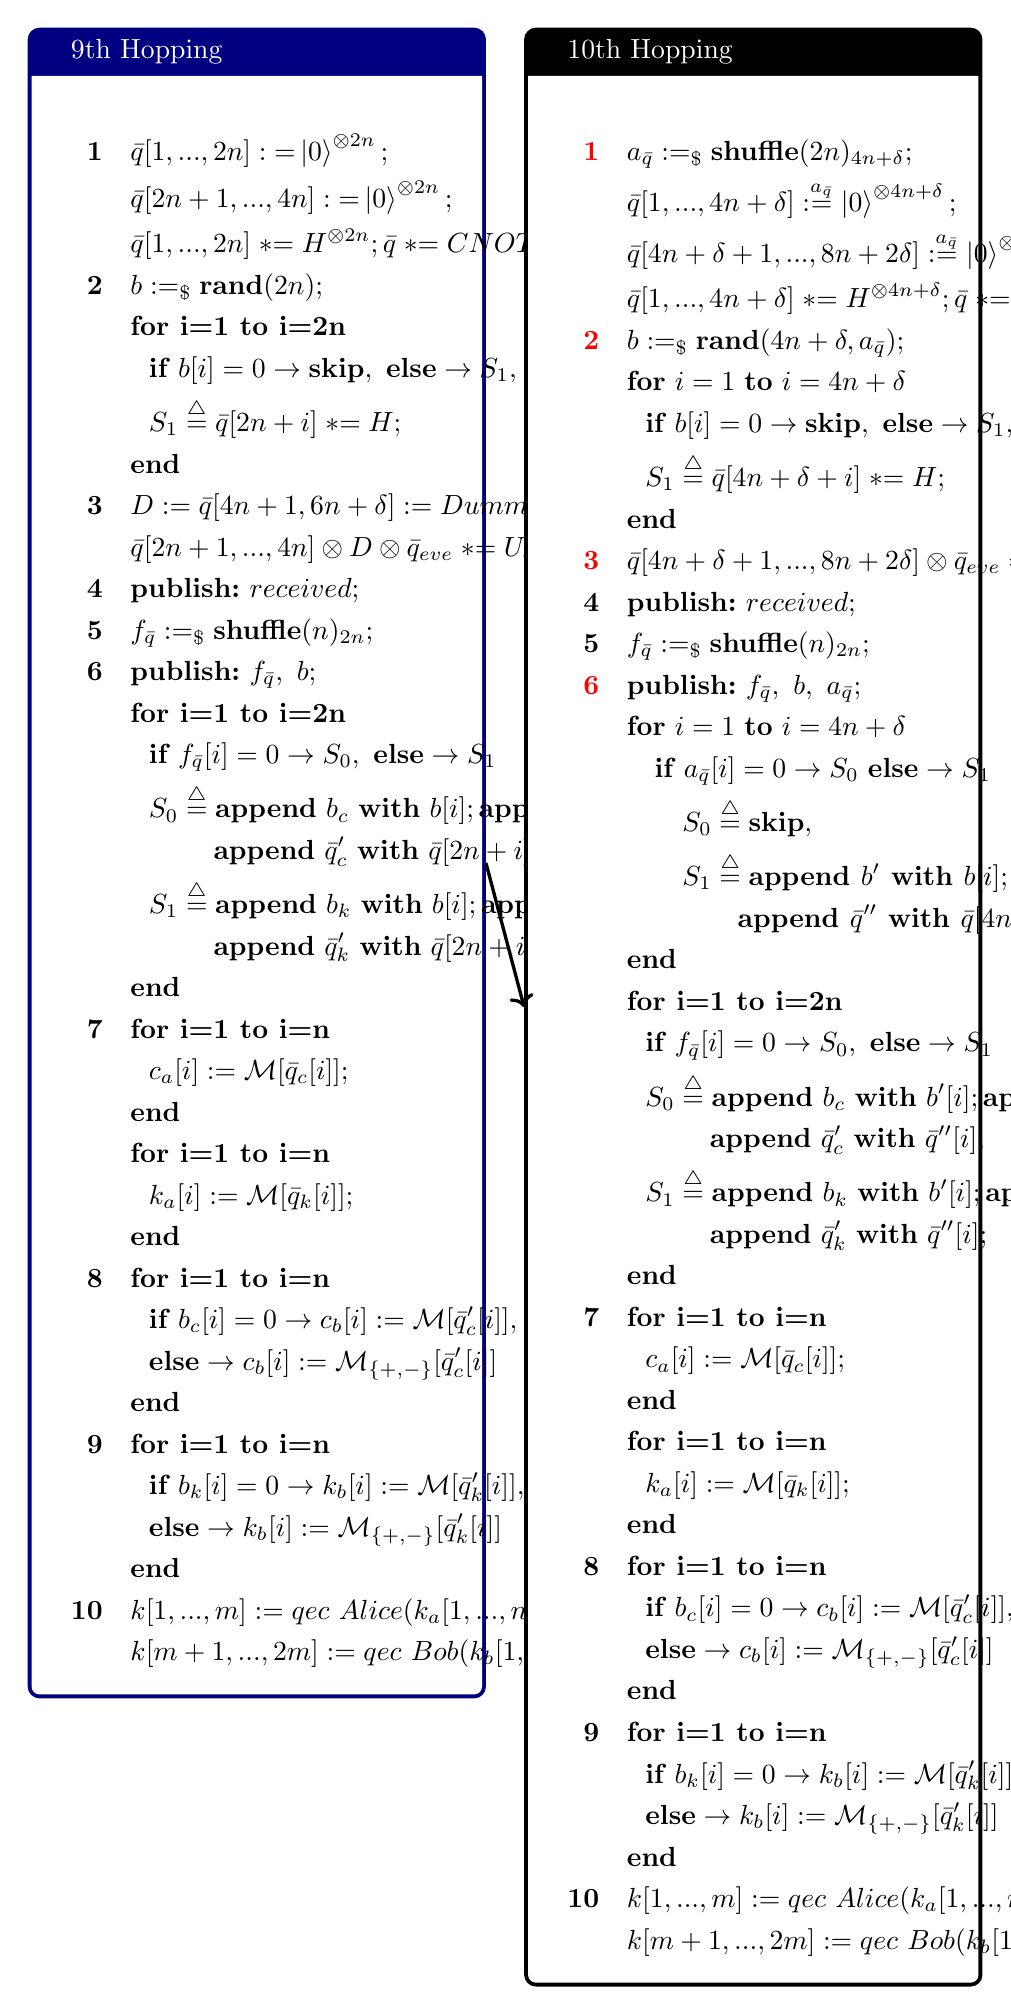
\begin{tikzpicture}[remember picture]

% Left box
\node[anchor=north west,inner sep=0pt,outer sep=0pt] (leftbox) at (0,0) {
\begin{minipage}[t]{0.48\textwidth}
\begin{tcolorbox}[colframe=blue!50!black, colback=white, title=9th Hopping, width=\textwidth]
\begin{align*}
    {\textbf{1}} \quad & \bar{q}[1,...,2n] :{=} \ket{0}^{\otimes 2n}; \\
    &\bar{q}[2n+1,...,4n] :{=} \ket{0}^{\otimes 2n};\\
    \quad &\bar{q}[1,...,2n] \asteq H^{\otimes 2n}; \bar{q} \asteq CNOT; \\
    \textbf{2} \quad & b :=_\$ \textbf{rand}(2n); \\
    &\textbf{for~i=1~to~i=2n}\\
    &~~ \textbf{if }  b[i] = 0 \rightarrow \textbf{skip},~\textbf{else}\rightarrow S_{1},\\
    &~~ S_{1}\stackrel{\triangle}{=}\bar{q}[2n+i] \asteq H ;\\
    &\textbf{end}\\
    {\textbf{3}} \quad & {D}:= \bar{q}[4n+1,6n+\delta]:=Dummy;\\
    &\bar{q}[2n+1,...,4n]\otimes {D} \otimes \bar{q}_{eve} \asteq U_{\textbf{channel}}; \\
    \textbf{4} \quad & \textbf{publish:}~ received;\\
    {\textbf{5}} \quad & f_{\bar{q}}:=_\$\textbf{shuffle}(n)_{2n}; \\
    {\textbf{6}} \quad & \textbf{publish:}~ f_{\bar{q}},~b;\\
    &\textbf{for~i=1~to~i=2n}\\
    &~~ \textbf{if }  f_{\bar{q}}[i] = 0 \rightarrow S_{0},~\textbf{else}\rightarrow S_{1}\\
    &~~ S_{0}\stackrel{\triangle}{=}\textbf{append}~b_c~\textbf{with}~b[i];\textbf{append}~\bar{q}_c~\textbf{with}~\bar{q}[i];\\
    &~~~~~~~~~\textbf{append}~\bar{q}'_c~\textbf{with}~\bar{q}[2n+i];\\
    &~~ S_{1}\stackrel{\triangle}{=}\textbf{append}~b_k~\textbf{with}~b[i];\textbf{append}~\bar{q}_k~\textbf{with}~\bar{q}[i];\\
    &~~~~~~~~~\textbf{append}~\bar{q}'_k~\textbf{with}~\bar{q}[2n+i];\\
    &\textbf{end}\\
    {\textbf{{7}}} \quad & \textbf{for~i=1~to~i=n}\\
    &~~ c_a[i]:= \mathcal{M} [\bar{q}_{c}[i]];\\
    &\textbf{end}\\
    & \textbf{for~i=1~to~i=n}\\
    &~~ k_a[i]:= \mathcal{M} [\bar{q}_{k}[i]];\\
    &\textbf{end}\\
    {\textbf{{8}}} 
    \quad 
    &\textbf{for~i=1~to~i=n}\\
    &~~ \textbf{if }  b_c[i] = 0 \rightarrow c_b[i]:= \mathcal{M} [\bar{q}'_{c}[i]] ,\\
    &~~\textbf{else}\rightarrow c_b[i]:= \mathcal{M}_{\{+,-\}} [\bar{q}'_{c}[i]]\\
    &\textbf{end}\\
    {\textbf{{9}}} \quad &\textbf{for~i=1~to~i=n}\\
    &~~ \textbf{if }  b_k[i] = 0 \rightarrow k_b[i]:= \mathcal{M} [\bar{q}'_{k}[i]] ,\\
    &~~\textbf{else}\rightarrow k_b[i]:= \mathcal{M}_{\{+,-\}} [\bar{q}'_{k}[i]]\\
    &\textbf{end}\\
    \textbf{{10}} \quad & k[1,...,m]:=qec~Alice(k_a[1,...,n])\\
    \quad & k[m+1,...,2m]:=qec~Bob(k_b[1,...,n])
\end{align*}
\end{tcolorbox}
\end{minipage}
};

% Right box
\node[anchor=north west,inner sep=0pt,outer sep=0pt] (rightbox) at (0.52\textwidth,0) {
\begin{minipage}[t]{0.48\textwidth}
\begin{tcolorbox}[colframe=black!50!black, colback=white, title=10th Hopping, width=\textwidth]
\begin{align*}
    \textcolor{red}{\textbf{1}} \quad &  a_{\bar{q}}:=_\$\textbf{shuffle}(2n)_{4n+\delta};\\
    &\bar{q}[1,...,4n+\delta] :\stackrel{a_{\bar{q}}}{=} \ket{0}^{\otimes 4n+\delta}; \\
    &\bar{q}[4n+\delta+1,...,8n+2\delta] :\stackrel{a_{\bar{q}}}{=} \ket{0}^{\otimes 4n+\delta};\\
    \quad &\bar{q}[1,...,4n+\delta] \asteq H^{\otimes 4n+\delta}; \bar{q} \asteq CNOT; \\
    \textcolor{red}{\textbf{2}} \quad & b :=_\$ \textbf{rand}(4n+\delta,a_{\bar{q}}); \\
    &\textbf{for}~i=1~\textbf{to}~i=4n+\delta\\
    &~~ \textbf{if }  b[i] = 0 \rightarrow \textbf{skip},~\textbf{else}\rightarrow S_{1},\\
    &~~ S_{1}\stackrel{\triangle}{=}\bar{q}[4n+\delta+i] \asteq H ;\\
    &\textbf{end}\\
    \textcolor{red}{\textbf{3}} \quad & \bar{q}[4n+\delta+1,...,8n+2\delta]\otimes \bar{q}_{eve} \asteq U_{\textbf{channel}}; \\
    \textbf{4} \quad & \textbf{publish:}~ received;\\
    {\textbf{5}} \quad & f_{\bar{q}}:=_\$\textbf{shuffle}(n)_{2n}; \\
    \textcolor{red}{\textbf{6}} \quad & \textbf{publish:}~ f_{\bar{q}},~b,~a_{\bar{q}};\\
    &\textbf{for}~i=1~\textbf{to}~i=4n+\delta\\
    &\quad \textbf{if }  a_{\bar{q}}[i] = 0 \rightarrow S_{0} ~\textbf{else} \rightarrow S_{1}\\
    &\qquad S_{0}\stackrel{\triangle}{=}\textbf{skip},\\
    &\qquad S_{1}\stackrel{\triangle}{=}\textbf{append } b' \textbf{ with } b[i];\textbf{append } \bar{q}' \textbf{ with } \bar{q}[i];\\
    &\qquad\qquad\textbf{append } \bar{q}'' \textbf{ with } \bar{q}[4n+\delta+i]\\
    &\textbf{end}\\
    &\textbf{for~i=1~to~i=2n}\\
    &~~ \textbf{if }  f_{\bar{q}}[i] = 0 \rightarrow S_{0},~\textbf{else}\rightarrow S_{1}\\
    &~~ S_{0}\stackrel{\triangle}{=}\textbf{append}~b_c~\textbf{with}~b'[i];\textbf{append}~\bar{q}_c~\textbf{with}~\bar{q}'[i];\\
    &~~~~~~~~~\textbf{append}~\bar{q}'_c~\textbf{with}~\bar{q}''[i];\\
    &~~ S_{1}\stackrel{\triangle}{=}\textbf{append}~b_k~\textbf{with}~b'[i];\textbf{append}~\bar{q}_k~\textbf{with}~\bar{q}'[i];\\
    &~~~~~~~~~\textbf{append}~\bar{q}'_k~\textbf{with}~\bar{q}''[i];\\
    &\textbf{end}\\
    {\textbf{{7}}} \quad & \textbf{for~i=1~to~i=n}\\
    &~~ c_a[i]:= \mathcal{M} [\bar{q}_{c}[i]];\\
    &\textbf{end}\\
    & \textbf{for~i=1~to~i=n}\\
    &~~ k_a[i]:= \mathcal{M} [\bar{q}_{k}[i]];\\
    &\textbf{end}\\
    {\textbf{{8}}} 
    \quad 
    &\textbf{for~i=1~to~i=n}\\
    &~~ \textbf{if }  b_c[i] = 0 \rightarrow c_b[i]:= \mathcal{M} [\bar{q}'_{c}[i]] ,\\
    &~~\textbf{else}\rightarrow c_b[i]:= \mathcal{M}_{\{+,-\}} [\bar{q}'_{c}[i]]\\
    &\textbf{end}\\
    {\textbf{{9}}} \quad &\textbf{for~i=1~to~i=n}\\
    &~~ \textbf{if }  b_k[i] = 0 \rightarrow k_b[i]:= \mathcal{M} [\bar{q}'_{k}[i]] ,\\
    &~~\textbf{else}\rightarrow k_b[i]:= \mathcal{M}_{\{+,-\}} [\bar{q}'_{k}[i]]\\
    &\textbf{end}\\
    \textbf{{10}} \quad & k[1,...,m]:=qec~Alice(k_a[1,...,n])\\
    \quad & k[m+1,...,2m]:=qec~Bob(k_b[1,...,n])
\end{align*}
\end{tcolorbox}
\end{minipage}
};

% Draw arrow between boxes
\draw[->, very thick] (leftbox.east) -- node[above]{} (rightbox.west);

\end{tikzpicture}
\newpage

\noindent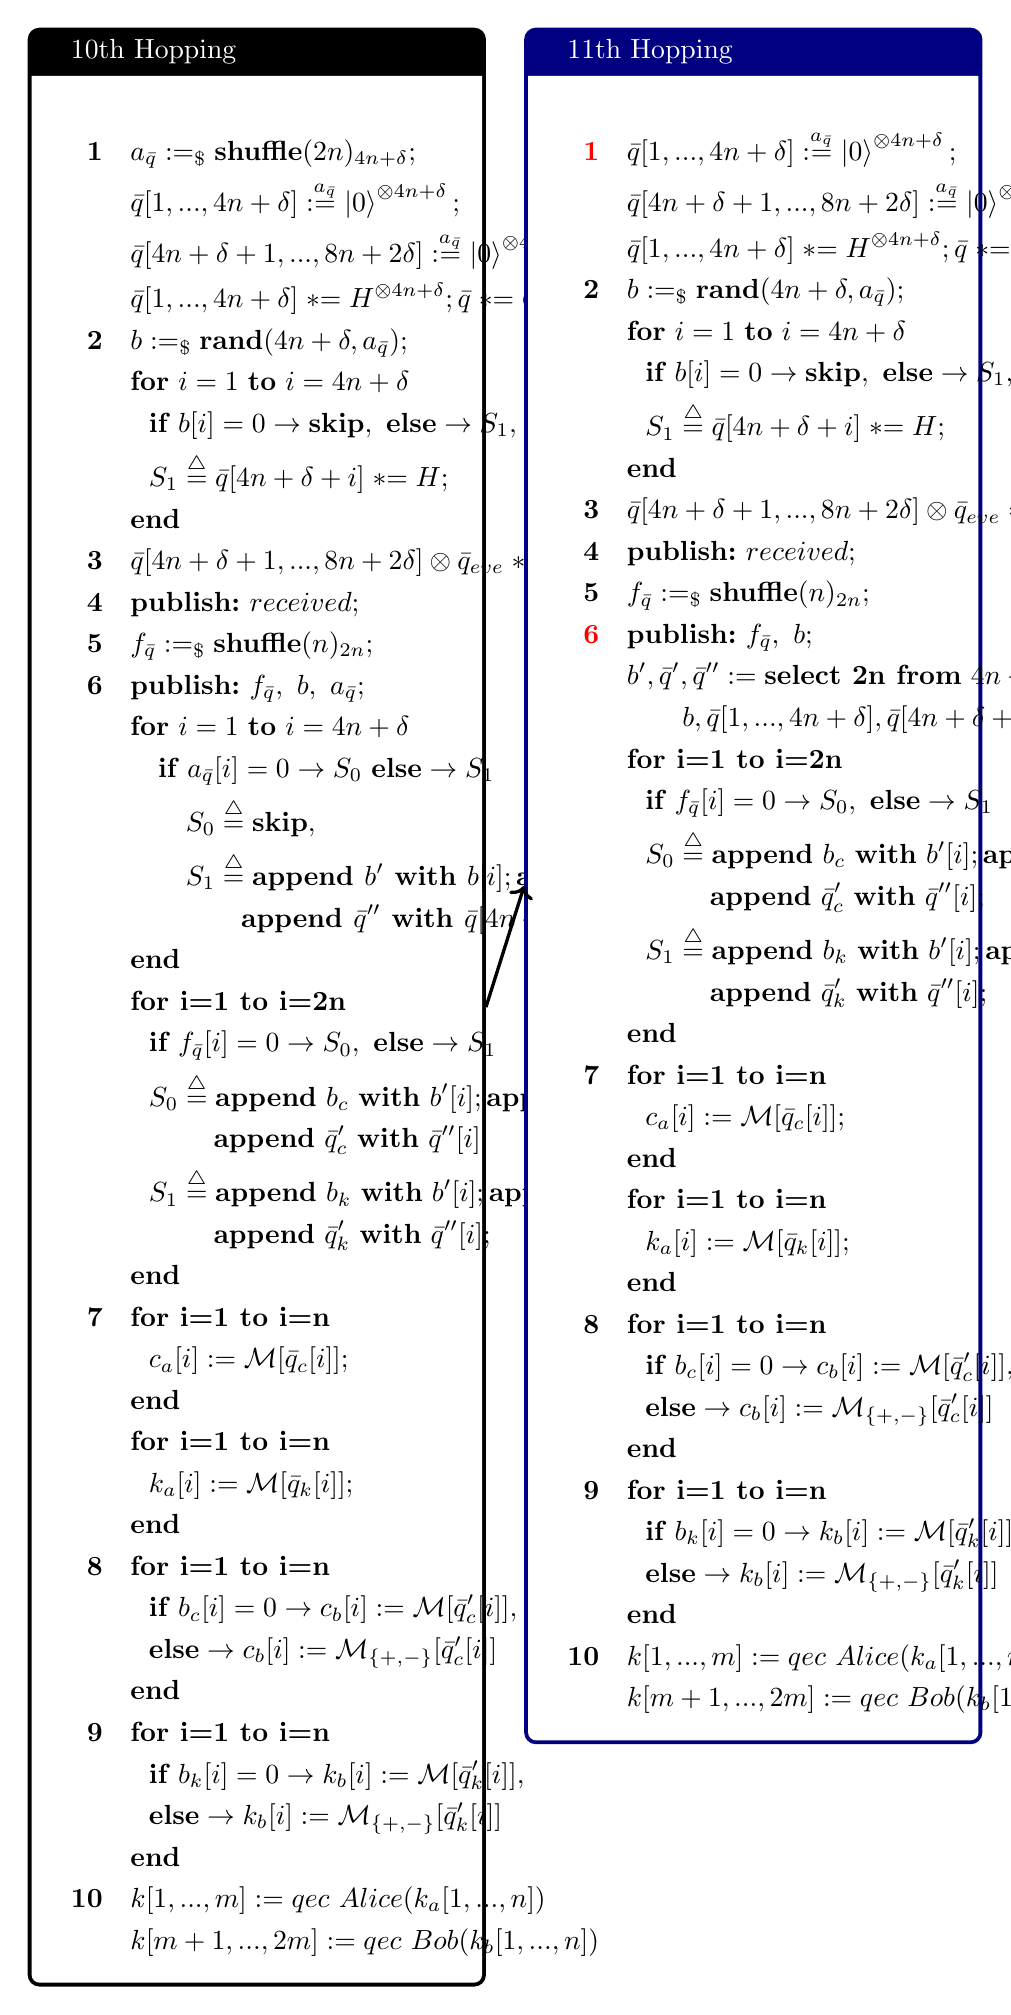
\begin{tikzpicture}[remember picture]

% Left box
\node[anchor=north west,inner sep=0pt,outer sep=0pt] (leftbox) at (0,0) {
\begin{minipage}[t]{0.48\textwidth}
\begin{tcolorbox}[colframe=black!50!black, colback=white, title=10th Hopping, width=\textwidth]
\begin{align*}
    {\textbf{1}} \quad &  a_{\bar{q}}:=_\$\textbf{shuffle}(2n)_{4n+\delta};\\
    &\bar{q}[1,...,4n+\delta] :\stackrel{a_{\bar{q}}}{=} \ket{0}^{\otimes 4n+\delta}; \\
    &\bar{q}[4n+\delta+1,...,8n+2\delta] :\stackrel{a_{\bar{q}}}{=} \ket{0}^{\otimes 4n+\delta};\\
    \quad &\bar{q}[1,...,4n+\delta] \asteq H^{\otimes 4n+\delta}; \bar{q} \asteq CNOT; \\
    {\textbf{2}} \quad & b :=_\$ \textbf{rand}(4n+\delta,a_{\bar{q}}); \\
    &\textbf{for}~i=1~\textbf{to}~i=4n+\delta\\
    &~~ \textbf{if }  b[i] = 0 \rightarrow \textbf{skip},~\textbf{else}\rightarrow S_{1},\\
    &~~ S_{1}\stackrel{\triangle}{=}\bar{q}[4n+\delta+i] \asteq H ;\\
    &\textbf{end}\\
    {\textbf{3}} \quad & \bar{q}[4n+\delta+1,...,8n+2\delta]\otimes \bar{q}_{eve} \asteq U_{\textbf{channel}}; \\
    \textbf{4} \quad & \textbf{publish:}~ received;\\
    {\textbf{5}} \quad & f_{\bar{q}}:=_\$\textbf{shuffle}(n)_{2n}; \\
    {\textbf{6}} \quad & \textbf{publish:}~ f_{\bar{q}},~b,~a_{\bar{q}};\\
    &\textbf{for}~i=1~\textbf{to}~i=4n+\delta\\
    &\quad \textbf{if }  a_{\bar{q}}[i] = 0 \rightarrow S_{0} ~\textbf{else} \rightarrow S_{1}\\
    &\qquad S_{0}\stackrel{\triangle}{=}\textbf{skip},\\
    &\qquad S_{1}\stackrel{\triangle}{=}\textbf{append } b' \textbf{ with } b[i];\textbf{append } \bar{q}' \textbf{ with } \bar{q}[i];\\
    &\qquad\qquad\textbf{append } \bar{q}'' \textbf{ with } \bar{q}[4n+\delta+i]\\
    &\textbf{end}\\
    &\textbf{for~i=1~to~i=2n}\\
    &~~ \textbf{if }  f_{\bar{q}}[i] = 0 \rightarrow S_{0},~\textbf{else}\rightarrow S_{1}\\
    &~~ S_{0}\stackrel{\triangle}{=}\textbf{append}~b_c~\textbf{with}~b'[i];\textbf{append}~\bar{q}_c~\textbf{with}~\bar{q}'[i];\\
    &~~~~~~~~~\textbf{append}~\bar{q}'_c~\textbf{with}~\bar{q}''[i];\\
    &~~ S_{1}\stackrel{\triangle}{=}\textbf{append}~b_k~\textbf{with}~b'[i];\textbf{append}~\bar{q}_k~\textbf{with}~\bar{q}'[i];\\
    &~~~~~~~~~\textbf{append}~\bar{q}'_k~\textbf{with}~\bar{q}''[i];\\
    &\textbf{end}\\
    {\textbf{{7}}} \quad & \textbf{for~i=1~to~i=n}\\
    &~~ c_a[i]:= \mathcal{M} [\bar{q}_{c}[i]];\\
    &\textbf{end}\\
    & \textbf{for~i=1~to~i=n}\\
    &~~ k_a[i]:= \mathcal{M} [\bar{q}_{k}[i]];\\
    &\textbf{end}\\
    {\textbf{{8}}} 
    \quad 
    &\textbf{for~i=1~to~i=n}\\
    &~~ \textbf{if }  b_c[i] = 0 \rightarrow c_b[i]:= \mathcal{M} [\bar{q}'_{c}[i]] ,\\
    &~~\textbf{else}\rightarrow c_b[i]:= \mathcal{M}_{\{+,-\}} [\bar{q}'_{c}[i]]\\
    &\textbf{end}\\
    {\textbf{{9}}} \quad &\textbf{for~i=1~to~i=n}\\
    &~~ \textbf{if }  b_k[i] = 0 \rightarrow k_b[i]:= \mathcal{M} [\bar{q}'_{k}[i]] ,\\
    &~~\textbf{else}\rightarrow k_b[i]:= \mathcal{M}_{\{+,-\}} [\bar{q}'_{k}[i]]\\
    &\textbf{end}\\
    \textbf{{10}} \quad & k[1,...,m]:=qec~Alice(k_a[1,...,n])\\
    \quad & k[m+1,...,2m]:=qec~Bob(k_b[1,...,n])
\end{align*}
\end{tcolorbox}
\end{minipage}
};

% Right box
\node[anchor=north west,inner sep=0pt,outer sep=0pt] (rightbox) at (0.52\textwidth,0) {
\begin{minipage}[t]{0.48\textwidth}
\begin{tcolorbox}[colframe=blue!50!black, colback=white, title=11th Hopping, width=\textwidth]
\begin{align*}
    \textcolor{red}{\textbf{1}} \quad 
    &\bar{q}[1,...,4n+\delta] :\stackrel{a_{\bar{q}}}{=} \ket{0}^{\otimes 4n+\delta}; \\
    &\bar{q}[4n+\delta+1,...,8n+2\delta] :\stackrel{a_{\bar{q}}}{=} \ket{0}^{\otimes 4n+\delta};\\
    \quad &\bar{q}[1,...,4n+\delta] \asteq H^{\otimes 4n+\delta}; \bar{q} \asteq CNOT; \\
    \textbf{2} \quad & b :=_\$ \textbf{rand}(4n+\delta,a_{\bar{q}}); \\
    &\textbf{for}~i=1~\textbf{to}~i=4n+\delta\\
    &~~ \textbf{if }  b[i] = 0 \rightarrow \textbf{skip},~\textbf{else}\rightarrow S_{1},\\
    &~~ S_{1}\stackrel{\triangle}{=}\bar{q}[4n+\delta+i] \asteq H ;\\
    &\textbf{end}\\
    {\textbf{3}} \quad & \bar{q}[4n+\delta+1,...,8n+2\delta]\otimes \bar{q}_{eve} \asteq U_{\textbf{channel}}; \\
    \textbf{4} \quad & \textbf{publish:}~ received;\\
    {\textbf{5}} \quad & f_{\bar{q}}:=_\$\textbf{shuffle}(n)_{2n}; \\
    \textcolor{red}{\textbf{6}} \quad & \textbf{publish:}~ f_{\bar{q}},~b;\\
    &b',\bar{q}',\bar{q}'':=\textbf{select 2n from}~4n+\delta ~\textbf{for}~\\
    &\qquad b,\bar{q}[1,...,4n+\delta],\bar{q}[4n+\delta+1,...,8n+2\delta];\\ 
    &\textbf{for~i=1~to~i=2n}\\
    &~~ \textbf{if }  f_{\bar{q}}[i] = 0 \rightarrow S_{0},~\textbf{else}\rightarrow S_{1}\\
    &~~ S_{0}\stackrel{\triangle}{=}\textbf{append}~b_c~\textbf{with}~b'[i];\textbf{append}~\bar{q}_c~\textbf{with}~\bar{q}'[i];\\
    &~~~~~~~~~\textbf{append}~\bar{q}'_c~\textbf{with}~\bar{q}''[i];\\
    &~~ S_{1}\stackrel{\triangle}{=}\textbf{append}~b_k~\textbf{with}~b'[i];\textbf{append}~\bar{q}_k~\textbf{with}~\bar{q}'[i];\\
    &~~~~~~~~~\textbf{append}~\bar{q}'_k~\textbf{with}~\bar{q}''[i];\\
    &\textbf{end}\\
    {\textbf{{7}}} \quad & \textbf{for~i=1~to~i=n}\\
    &~~ c_a[i]:= \mathcal{M} [\bar{q}_{c}[i]];\\
    &\textbf{end}\\
    & \textbf{for~i=1~to~i=n}\\
    &~~ k_a[i]:= \mathcal{M} [\bar{q}_{k}[i]];\\
    &\textbf{end}\\
    {\textbf{{8}}} 
    \quad 
    &\textbf{for~i=1~to~i=n}\\
    &~~ \textbf{if }  b_c[i] = 0 \rightarrow c_b[i]:= \mathcal{M} [\bar{q}'_{c}[i]] ,\\
    &~~\textbf{else}\rightarrow c_b[i]:= \mathcal{M}_{\{+,-\}} [\bar{q}'_{c}[i]]\\
    &\textbf{end}\\
    {\textbf{{9}}} \quad &\textbf{for~i=1~to~i=n}\\
    &~~ \textbf{if }  b_k[i] = 0 \rightarrow k_b[i]:= \mathcal{M} [\bar{q}'_{k}[i]] ,\\
    &~~\textbf{else}\rightarrow k_b[i]:= \mathcal{M}_{\{+,-\}} [\bar{q}'_{k}[i]]\\
    &\textbf{end}\\
    \textbf{{10}} \quad & k[1,...,m]:=qec~Alice(k_a[1,...,n])\\
    \quad & k[m+1,...,2m]:=qec~Bob(k_b[1,...,n])
\end{align*}
\end{tcolorbox}
\end{minipage}
};

% Draw arrow between boxes
\draw[->, very thick] (leftbox.east) -- node[above]{} (rightbox.west);

\end{tikzpicture}
\newpage

\noindent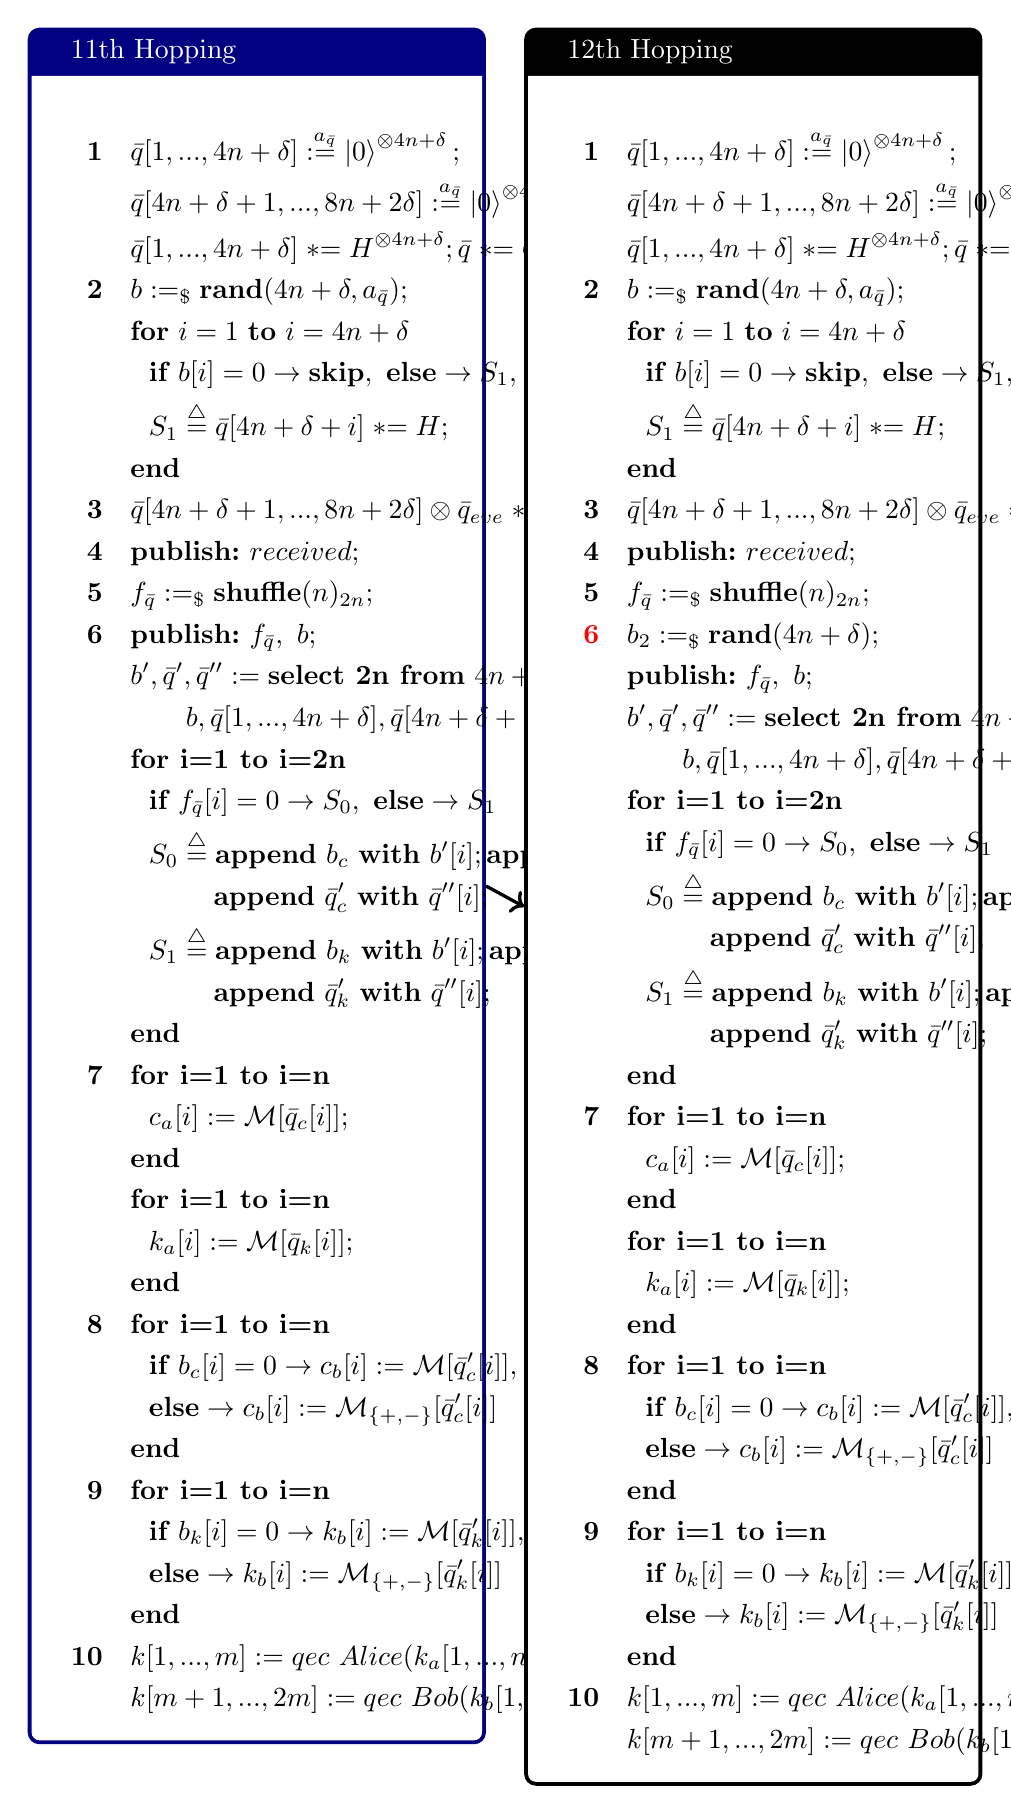
\begin{tikzpicture}[remember picture]

% Left box
\node[anchor=north west,inner sep=0pt,outer sep=0pt] (leftbox) at (0,0) {
\begin{minipage}[t]{0.48\textwidth}
\begin{tcolorbox}[colframe=blue!50!black, colback=white, title=11th Hopping, width=\textwidth]
\begin{align*}
    {\textbf{1}} \quad 
    &\bar{q}[1,...,4n+\delta] :\stackrel{a_{\bar{q}}}{=} \ket{0}^{\otimes 4n+\delta}; \\
    &\bar{q}[4n+\delta+1,...,8n+2\delta] :\stackrel{a_{\bar{q}}}{=} \ket{0}^{\otimes 4n+\delta};\\
    \quad &\bar{q}[1,...,4n+\delta] \asteq H^{\otimes 4n+\delta}; \bar{q} \asteq CNOT; \\
    \textbf{2} \quad & b :=_\$ \textbf{rand}(4n+\delta,a_{\bar{q}}); \\
    &\textbf{for}~i=1~\textbf{to}~i=4n+\delta\\
    &~~ \textbf{if }  b[i] = 0 \rightarrow \textbf{skip},~\textbf{else}\rightarrow S_{1},\\
    &~~ S_{1}\stackrel{\triangle}{=}\bar{q}[4n+\delta+i] \asteq H ;\\
    &\textbf{end}\\
    {\textbf{3}} \quad & \bar{q}[4n+\delta+1,...,8n+2\delta]\otimes \bar{q}_{eve} \asteq U_{\textbf{channel}}; \\
    \textbf{4} \quad & \textbf{publish:}~ received;\\
    {\textbf{5}} \quad & f_{\bar{q}}:=_\$\textbf{shuffle}(n)_{2n}; \\
    {\textbf{6}} \quad & \textbf{publish:}~ f_{\bar{q}},~b;\\
    &b',\bar{q}',\bar{q}'':=\textbf{select 2n from}~4n+\delta ~\textbf{for}~\\
    &\qquad b,\bar{q}[1,...,4n+\delta],\bar{q}[4n+\delta+1,...,8n+2\delta];\\ 
    &\textbf{for~i=1~to~i=2n}\\
    &~~ \textbf{if }  f_{\bar{q}}[i] = 0 \rightarrow S_{0},~\textbf{else}\rightarrow S_{1}\\
    &~~ S_{0}\stackrel{\triangle}{=}\textbf{append}~b_c~\textbf{with}~b'[i];\textbf{append}~\bar{q}_c~\textbf{with}~\bar{q}'[i];\\
    &~~~~~~~~~\textbf{append}~\bar{q}'_c~\textbf{with}~\bar{q}''[i];\\
    &~~ S_{1}\stackrel{\triangle}{=}\textbf{append}~b_k~\textbf{with}~b'[i];\textbf{append}~\bar{q}_k~\textbf{with}~\bar{q}'[i];\\
    &~~~~~~~~~\textbf{append}~\bar{q}'_k~\textbf{with}~\bar{q}''[i];\\
    &\textbf{end}\\
    {\textbf{{7}}} \quad & \textbf{for~i=1~to~i=n}\\
    &~~ c_a[i]:= \mathcal{M} [\bar{q}_{c}[i]];\\
    &\textbf{end}\\
    & \textbf{for~i=1~to~i=n}\\
    &~~ k_a[i]:= \mathcal{M} [\bar{q}_{k}[i]];\\
    &\textbf{end}\\
    {\textbf{{8}}} 
    \quad 
    &\textbf{for~i=1~to~i=n}\\
    &~~ \textbf{if }  b_c[i] = 0 \rightarrow c_b[i]:= \mathcal{M} [\bar{q}'_{c}[i]] ,\\
    &~~\textbf{else}\rightarrow c_b[i]:= \mathcal{M}_{\{+,-\}} [\bar{q}'_{c}[i]]\\
    &\textbf{end}\\
    {\textbf{{9}}} \quad &\textbf{for~i=1~to~i=n}\\
    &~~ \textbf{if }  b_k[i] = 0 \rightarrow k_b[i]:= \mathcal{M} [\bar{q}'_{k}[i]] ,\\
    &~~\textbf{else}\rightarrow k_b[i]:= \mathcal{M}_{\{+,-\}} [\bar{q}'_{k}[i]]\\
    &\textbf{end}\\
    \textbf{{10}} \quad & k[1,...,m]:=qec~Alice(k_a[1,...,n])\\
    \quad & k[m+1,...,2m]:=qec~Bob(k_b[1,...,n])
\end{align*}
\end{tcolorbox}
\end{minipage}
};

% Right box
\node[anchor=north west,inner sep=0pt,outer sep=0pt] (rightbox) at (0.52\textwidth,0) {
\begin{minipage}[t]{0.48\textwidth}
\begin{tcolorbox}[colframe=black!50!black, colback=white, title=12th Hopping, width=\textwidth]
\begin{align*}
    {\textbf{1}} \quad 
    &\bar{q}[1,...,4n+\delta] :\stackrel{a_{\bar{q}}}{=} \ket{0}^{\otimes 4n+\delta}; \\
    &\bar{q}[4n+\delta+1,...,8n+2\delta] :\stackrel{a_{\bar{q}}}{=} \ket{0}^{\otimes 4n+\delta};\\
    \quad &\bar{q}[1,...,4n+\delta] \asteq H^{\otimes 4n+\delta}; \bar{q} \asteq CNOT; \\
    \textbf{2} \quad & b :=_\$ \textbf{rand}(4n+\delta,a_{\bar{q}}); \\
    &\textbf{for}~i=1~\textbf{to}~i=4n+\delta\\
    &~~ \textbf{if }  b[i] = 0 \rightarrow \textbf{skip},~\textbf{else}\rightarrow S_{1},\\
    &~~ S_{1}\stackrel{\triangle}{=}\bar{q}[4n+\delta+i] \asteq H ;\\
    &\textbf{end}\\
    {\textbf{3}} \quad & \bar{q}[4n+\delta+1,...,8n+2\delta]\otimes \bar{q}_{eve} \asteq U_{\textbf{channel}}; \\
    \textbf{4} \quad & \textbf{publish:}~ received;\\
    {\textbf{5}} \quad & f_{\bar{q}}:=_\$\textbf{shuffle}(n)_{2n}; \\
    \textcolor{red}{\textbf{6}} \quad & 
    b_2:=_{\$}\textbf{rand}(4n+\delta);\\&\textbf{publish:}~ f_{\bar{q}},~b;\\
    &b',\bar{q}',\bar{q}'':=\textbf{select 2n from}~4n+\delta ~\textbf{for}~\\
    &\qquad b,\bar{q}[1,...,4n+\delta],\bar{q}[4n+\delta+1,...,8n+2\delta];\\ 
    &\textbf{for~i=1~to~i=2n}\\
    &~~ \textbf{if }  f_{\bar{q}}[i] = 0 \rightarrow S_{0},~\textbf{else}\rightarrow S_{1}\\
    &~~ S_{0}\stackrel{\triangle}{=}\textbf{append}~b_c~\textbf{with}~b'[i];\textbf{append}~\bar{q}_c~\textbf{with}~\bar{q}'[i];\\
    &~~~~~~~~~\textbf{append}~\bar{q}'_c~\textbf{with}~\bar{q}''[i];\\
    &~~ S_{1}\stackrel{\triangle}{=}\textbf{append}~b_k~\textbf{with}~b'[i];\textbf{append}~\bar{q}_k~\textbf{with}~\bar{q}'[i];\\
    &~~~~~~~~~\textbf{append}~\bar{q}'_k~\textbf{with}~\bar{q}''[i];\\
    &\textbf{end}\\
    {\textbf{{7}}} \quad & \textbf{for~i=1~to~i=n}\\
    &~~ c_a[i]:= \mathcal{M} [\bar{q}_{c}[i]];\\
    &\textbf{end}\\
    & \textbf{for~i=1~to~i=n}\\
    &~~ k_a[i]:= \mathcal{M} [\bar{q}_{k}[i]];\\
    &\textbf{end}\\
    {\textbf{{8}}} 
    \quad 
    &\textbf{for~i=1~to~i=n}\\
    &~~ \textbf{if }  b_c[i] = 0 \rightarrow c_b[i]:= \mathcal{M} [\bar{q}'_{c}[i]] ,\\
    &~~\textbf{else}\rightarrow c_b[i]:= \mathcal{M}_{\{+,-\}} [\bar{q}'_{c}[i]]\\
    &\textbf{end}\\
    {\textbf{{9}}} \quad &\textbf{for~i=1~to~i=n}\\
    &~~ \textbf{if }  b_k[i] = 0 \rightarrow k_b[i]:= \mathcal{M} [\bar{q}'_{k}[i]] ,\\
    &~~\textbf{else}\rightarrow k_b[i]:= \mathcal{M}_{\{+,-\}} [\bar{q}'_{k}[i]]\\
    &\textbf{end}\\
    \textbf{{10}} \quad & k[1,...,m]:=qec~Alice(k_a[1,...,n])\\
    \quad & k[m+1,...,2m]:=qec~Bob(k_b[1,...,n])
\end{align*}
\end{tcolorbox}
\end{minipage}
};

% Draw arrow between boxes
\draw[->, very thick] (leftbox.east) -- node[above]{} (rightbox.west);

\end{tikzpicture}
\newpage


\noindent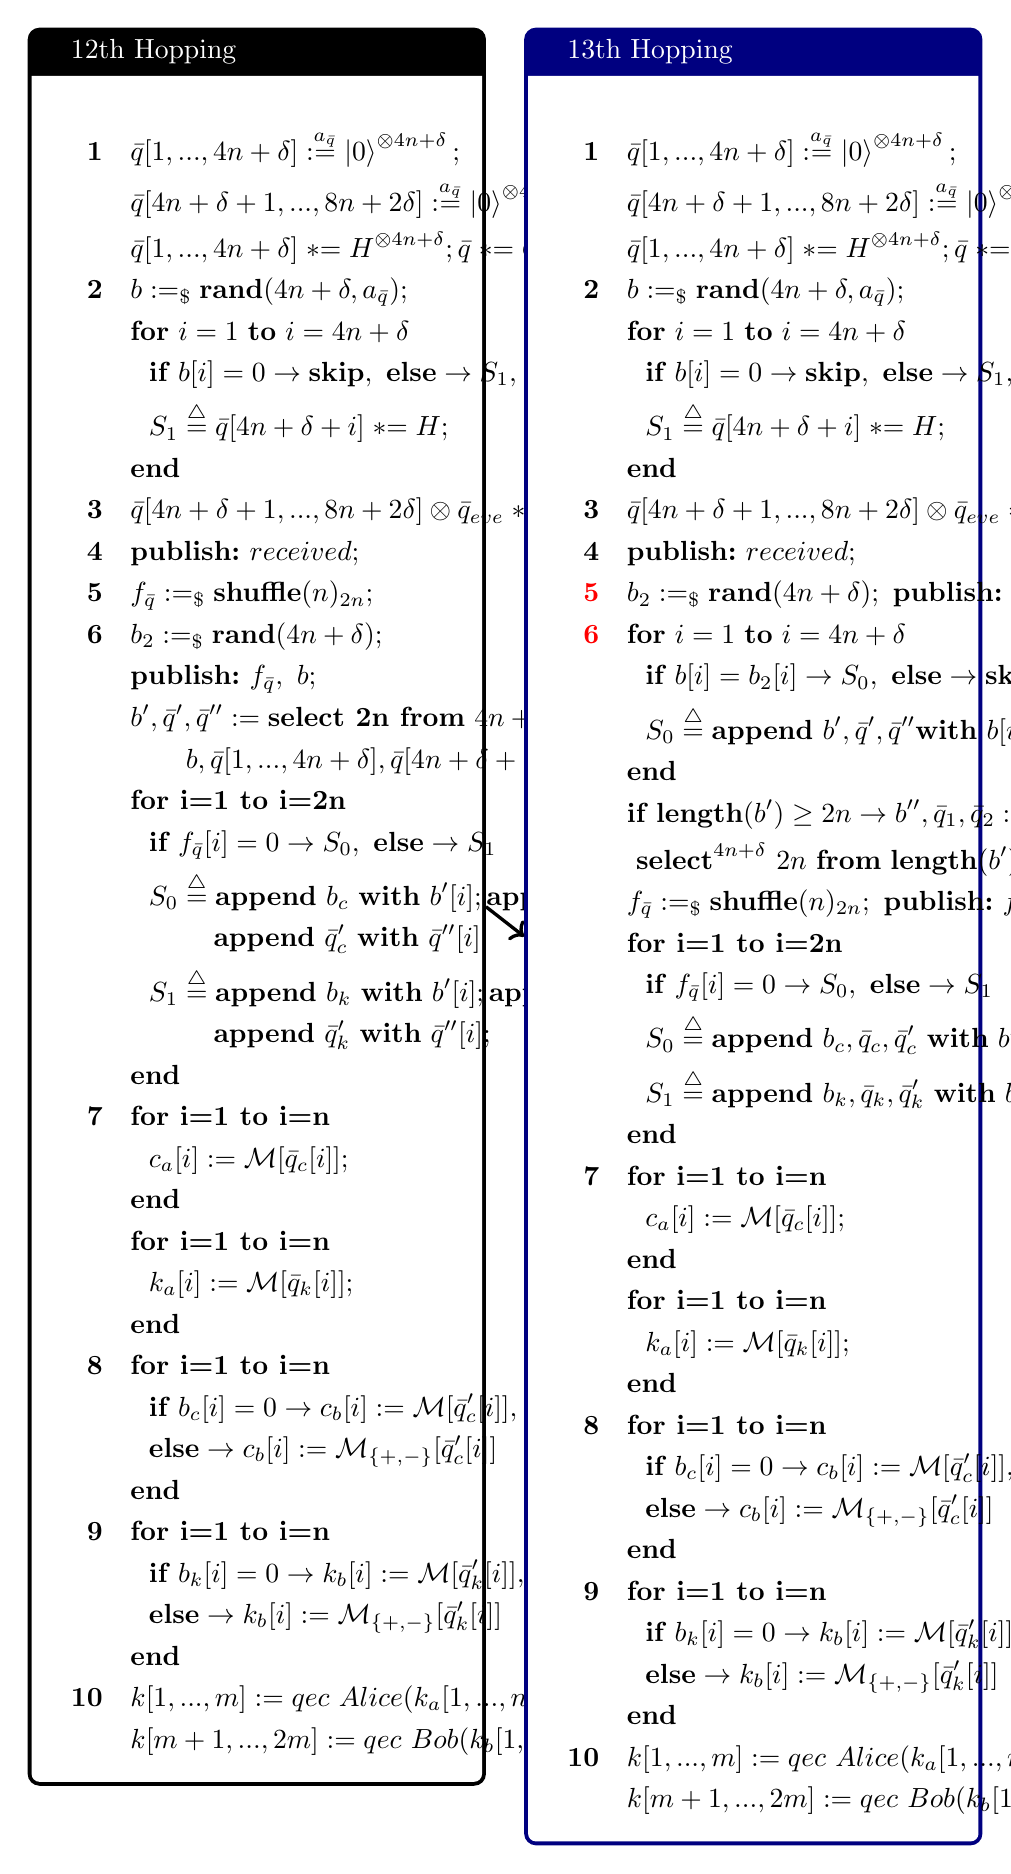
\begin{tikzpicture}[remember picture]

% Left box
\node[anchor=north west,inner sep=0pt,outer sep=0pt] (leftbox) at (0,0) {
\begin{minipage}[t]{0.48\textwidth}
\begin{tcolorbox}[colframe=black!50!black, colback=white, title=12th Hopping, width=\textwidth]
\begin{align*}
    {\textbf{1}} \quad 
    &\bar{q}[1,...,4n+\delta] :\stackrel{a_{\bar{q}}}{=} \ket{0}^{\otimes 4n+\delta}; \\
    &\bar{q}[4n+\delta+1,...,8n+2\delta] :\stackrel{a_{\bar{q}}}{=} \ket{0}^{\otimes 4n+\delta};\\
    \quad &\bar{q}[1,...,4n+\delta] \asteq H^{\otimes 4n+\delta}; \bar{q} \asteq CNOT; \\
    \textbf{2} \quad & b :=_\$ \textbf{rand}(4n+\delta,a_{\bar{q}}); \\
    &\textbf{for}~i=1~\textbf{to}~i=4n+\delta\\
    &~~ \textbf{if }  b[i] = 0 \rightarrow \textbf{skip},~\textbf{else}\rightarrow S_{1},\\
    &~~ S_{1}\stackrel{\triangle}{=}\bar{q}[4n+\delta+i] \asteq H ;\\
    &\textbf{end}\\
    {\textbf{3}} \quad & \bar{q}[4n+\delta+1,...,8n+2\delta]\otimes \bar{q}_{eve} \asteq U_{\textbf{channel}}; \\
    \textbf{4} \quad & \textbf{publish:}~ received;\\
    {\textbf{5}} \quad & f_{\bar{q}}:=_\$\textbf{shuffle}(n)_{2n}; \\
    {\textbf{6}} \quad & 
    b_2:=_{\$}\textbf{rand}(4n+\delta);\\&\textbf{publish:}~ f_{\bar{q}},~b;\\
    &b',\bar{q}',\bar{q}'':=\textbf{select 2n from}~4n+\delta ~\textbf{for}~\\
    &\qquad b,\bar{q}[1,...,4n+\delta],\bar{q}[4n+\delta+1,...,8n+2\delta];\\ 
    &\textbf{for~i=1~to~i=2n}\\
    &~~ \textbf{if }  f_{\bar{q}}[i] = 0 \rightarrow S_{0},~\textbf{else}\rightarrow S_{1}\\
    &~~ S_{0}\stackrel{\triangle}{=}\textbf{append}~b_c~\textbf{with}~b'[i];\textbf{append}~\bar{q}_c~\textbf{with}~\bar{q}'[i];\\
    &~~~~~~~~~\textbf{append}~\bar{q}'_c~\textbf{with}~\bar{q}''[i];\\
    &~~ S_{1}\stackrel{\triangle}{=}\textbf{append}~b_k~\textbf{with}~b'[i];\textbf{append}~\bar{q}_k~\textbf{with}~\bar{q}'[i];\\
    &~~~~~~~~~\textbf{append}~\bar{q}'_k~\textbf{with}~\bar{q}''[i];\\
    &\textbf{end}\\
    {\textbf{{7}}} \quad & \textbf{for~i=1~to~i=n}\\
    &~~ c_a[i]:= \mathcal{M} [\bar{q}_{c}[i]];\\
    &\textbf{end}\\
    & \textbf{for~i=1~to~i=n}\\
    &~~ k_a[i]:= \mathcal{M} [\bar{q}_{k}[i]];\\
    &\textbf{end}\\
    {\textbf{{8}}} 
    \quad 
    &\textbf{for~i=1~to~i=n}\\
    &~~ \textbf{if }  b_c[i] = 0 \rightarrow c_b[i]:= \mathcal{M} [\bar{q}'_{c}[i]] ,\\
    &~~\textbf{else}\rightarrow c_b[i]:= \mathcal{M}_{\{+,-\}} [\bar{q}'_{c}[i]]\\
    &\textbf{end}\\
    {\textbf{{9}}} \quad &\textbf{for~i=1~to~i=n}\\
    &~~ \textbf{if }  b_k[i] = 0 \rightarrow k_b[i]:= \mathcal{M} [\bar{q}'_{k}[i]] ,\\
    &~~\textbf{else}\rightarrow k_b[i]:= \mathcal{M}_{\{+,-\}} [\bar{q}'_{k}[i]]\\
    &\textbf{end}\\
    \textbf{{10}} \quad & k[1,...,m]:=qec~Alice(k_a[1,...,n])\\
    \quad & k[m+1,...,2m]:=qec~Bob(k_b[1,...,n])
\end{align*}
\end{tcolorbox}
\end{minipage}
};

% Right box
\node[anchor=north west,inner sep=0pt,outer sep=0pt] (rightbox) at (0.52\textwidth,0) {
\begin{minipage}[t]{0.48\textwidth}
\begin{tcolorbox}[colframe=blue!50!black, colback=white, title=13th Hopping, width=\textwidth]
\begin{align*}
    {\textbf{1}} \quad 
    &\bar{q}[1,...,4n+\delta] :\stackrel{a_{\bar{q}}}{=} \ket{0}^{\otimes 4n+\delta}; \\
    &\bar{q}[4n+\delta+1,...,8n+2\delta] :\stackrel{a_{\bar{q}}}{=} \ket{0}^{\otimes 4n+\delta};\\
    \quad &\bar{q}[1,...,4n+\delta] \asteq H^{\otimes 4n+\delta}; \bar{q} \asteq CNOT; \\
    \textbf{2} \quad & b :=_\$ \textbf{rand}(4n+\delta,a_{\bar{q}}); \\
    &\textbf{for}~i=1~\textbf{to}~i=4n+\delta\\
    &~~ \textbf{if }  b[i] = 0 \rightarrow \textbf{skip},~\textbf{else}\rightarrow S_{1},\\
    &~~ S_{1}\stackrel{\triangle}{=}\bar{q}[4n+\delta+i] \asteq H ;\\
    &\textbf{end}\\
    {\textbf{3}} \quad & \bar{q}[4n+\delta+1,...,8n+2\delta]\otimes \bar{q}_{eve} \asteq U_{\textbf{channel}}; \\
    \textbf{4} \quad & \textbf{publish:}~ received;\\
    \textcolor{red}{\textbf{5}} \quad & b_2 :=_\$ \textbf{rand}(4n+\delta); ~\textbf{publish:}~ b;\\
    \textcolor{red}{\textbf{6}} \quad &\textbf{for} ~i=1 ~\textbf{to} ~i=4n+\delta\\
    &~~ \textbf{if } b[i]= b_2[i] \rightarrow S_{0},~\textbf{else}\rightarrow\textbf{skip}~, \\
    &~~ S_{0}\stackrel{\triangle}{=}\textbf{append}~b',\bar{q}',\bar{q}''\textbf{with}~b[i],\bar{q}[i],\bar{q}[i+4n+\delta];\\
    &\textbf{end}\\
    &{\textbf{if }} \textbf{length} (b')\geq 2n\rightarrow b'',\bar{q}_1,\bar{q}_2:=\\&~\textbf{select}^{4n+\delta}~2n~\textbf{from}~\textbf{length}(b')~\textbf{for}~b',\bar{q}',\bar{q}'';\\
    & f_{\bar{q}}:=_\$\textbf{shuffle}(n)_{2n}; ~ \textbf{publish:}~ f_{\bar{q}};\\ 
    &\textbf{for~i=1~to~i=2n}\\
    &~~ \textbf{if }  f_{\bar{q}}[i] = 0 \rightarrow S_{0},~\textbf{else}\rightarrow S_{1}\\
    &~~ S_{0}\stackrel{\triangle}{=}\textbf{append}~b_c,\bar{q}_c,\bar{q}'_c~\textbf{with}~b''[i],\bar{q}_1[i],\bar{q}_2[i];\\
    &~~ S_{1}\stackrel{\triangle}{=}\textbf{append}~b_k,\bar{q}_k,\bar{q}'_k~\textbf{with}~b''[i],\bar{q}_1[i],\bar{q}_2[i];\\
    &\textbf{end}\\
    {\textbf{{7}}} \quad & \textbf{for~i=1~to~i=n}\\
    &~~ c_a[i]:= \mathcal{M} [\bar{q}_{c}[i]];\\
    &\textbf{end}\\
    & \textbf{for~i=1~to~i=n}\\
    &~~ k_a[i]:= \mathcal{M} [\bar{q}_{k}[i]];\\
    &\textbf{end}\\
    {\textbf{{8}}} 
    \quad 
    &\textbf{for~i=1~to~i=n}\\
    &~~ \textbf{if }  b_c[i] = 0 \rightarrow c_b[i]:= \mathcal{M} [\bar{q}'_{c}[i]] ,\\
    &~~\textbf{else}\rightarrow c_b[i]:= \mathcal{M}_{\{+,-\}} [\bar{q}'_{c}[i]]\\
    &\textbf{end}\\
    {\textbf{{9}}} \quad &\textbf{for~i=1~to~i=n}\\
    &~~ \textbf{if }  b_k[i] = 0 \rightarrow k_b[i]:= \mathcal{M} [\bar{q}'_{k}[i]] ,\\
    &~~\textbf{else}\rightarrow k_b[i]:= \mathcal{M}_{\{+,-\}} [\bar{q}'_{k}[i]]\\
    &\textbf{end}\\
    \textbf{{10}} \quad & k[1,...,m]:=qec~Alice(k_a[1,...,n])\\
    \quad & k[m+1,...,2m]:=qec~Bob(k_b[1,...,n])
\end{align*}
\end{tcolorbox}
\end{minipage}
};

% Draw arrow between boxes
\draw[->, very thick] (leftbox.east) -- node[above]{} (rightbox.west);

\end{tikzpicture}
\newpage

\noindent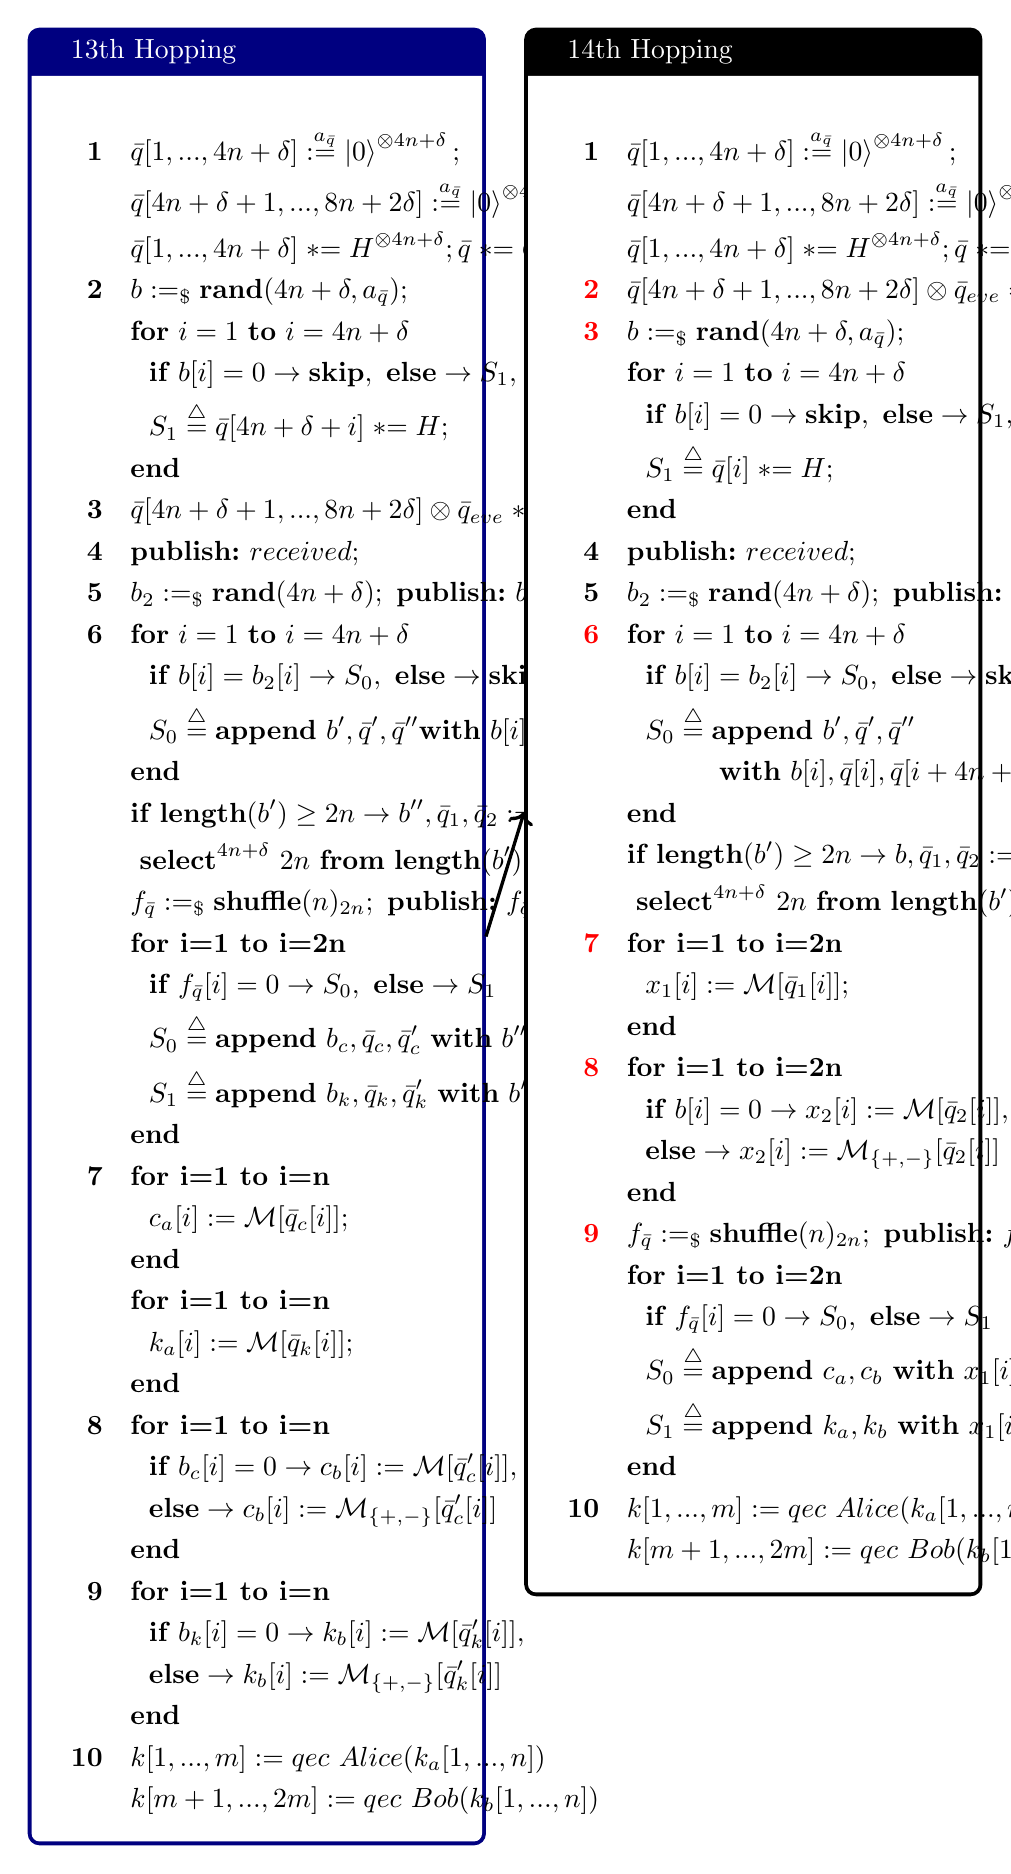
\begin{tikzpicture}[remember picture]

% Left box
\node[anchor=north west,inner sep=0pt,outer sep=0pt] (leftbox) at (0,0) {
\begin{minipage}[t]{0.48\textwidth}
\begin{tcolorbox}[colframe=blue!50!black, colback=white, title=13th Hopping, width=\textwidth]
\begin{align*}
    {\textbf{1}} \quad 
    &\bar{q}[1,...,4n+\delta] :\stackrel{a_{\bar{q}}}{=} \ket{0}^{\otimes 4n+\delta}; \\
    &\bar{q}[4n+\delta+1,...,8n+2\delta] :\stackrel{a_{\bar{q}}}{=} \ket{0}^{\otimes 4n+\delta};\\
    \quad &\bar{q}[1,...,4n+\delta] \asteq H^{\otimes 4n+\delta}; \bar{q} \asteq CNOT; \\
    \textbf{2} \quad & b :=_\$ \textbf{rand}(4n+\delta,a_{\bar{q}}); \\
    &\textbf{for}~i=1~\textbf{to}~i=4n+\delta\\
    &~~ \textbf{if }  b[i] = 0 \rightarrow \textbf{skip},~\textbf{else}\rightarrow S_{1},\\
    &~~ S_{1}\stackrel{\triangle}{=}\bar{q}[4n+\delta+i] \asteq H ;\\
    &\textbf{end}\\
    {\textbf{3}} \quad & \bar{q}[4n+\delta+1,...,8n+2\delta]\otimes \bar{q}_{eve} \asteq U_{\textbf{channel}}; \\
    \textbf{4} \quad & \textbf{publish:}~ received;\\
    {\textbf{5}} \quad & b_2 :=_\$ \textbf{rand}(4n+\delta); ~\textbf{publish:}~ b;\\
    {\textbf{6}} \quad &\textbf{for} ~i=1 ~\textbf{to} ~i=4n+\delta\\
    &~~ \textbf{if } b[i]= b_2[i] \rightarrow S_{0},~\textbf{else}\rightarrow\textbf{skip}~, \\
    &~~ S_{0}\stackrel{\triangle}{=}\textbf{append}~b',\bar{q}',\bar{q}''\textbf{with}~b[i],\bar{q}[i],\bar{q}[i+4n+\delta];\\
    &\textbf{end}\\
    &{\textbf{if }} \textbf{length} (b')\geq 2n\rightarrow b'',\bar{q}_1,\bar{q}_2:=\\&~\textbf{select}^{4n+\delta}~2n~\textbf{from}~\textbf{length}(b')~\textbf{for}~b',\bar{q}',\bar{q}'';\\
    & f_{\bar{q}}:=_\$\textbf{shuffle}(n)_{2n}; ~ \textbf{publish:}~ f_{\bar{q}};\\ 
    &\textbf{for~i=1~to~i=2n}\\
    &~~ \textbf{if }  f_{\bar{q}}[i] = 0 \rightarrow S_{0},~\textbf{else}\rightarrow S_{1}\\
    &~~ S_{0}\stackrel{\triangle}{=}\textbf{append}~b_c,\bar{q}_c,\bar{q}'_c~\textbf{with}~b''[i],\bar{q}_1[i],\bar{q}_2[i];\\
    &~~ S_{1}\stackrel{\triangle}{=}\textbf{append}~b_k,\bar{q}_k,\bar{q}'_k~\textbf{with}~b''[i],\bar{q}_1[i],\bar{q}_2[i];\\
    &\textbf{end}\\
    {\textbf{{7}}} \quad & \textbf{for~i=1~to~i=n}\\
    &~~ c_a[i]:= \mathcal{M} [\bar{q}_{c}[i]];\\
    &\textbf{end}\\
    & \textbf{for~i=1~to~i=n}\\
    &~~ k_a[i]:= \mathcal{M} [\bar{q}_{k}[i]];\\
    &\textbf{end}\\
    {\textbf{{8}}} 
    \quad 
    &\textbf{for~i=1~to~i=n}\\
    &~~ \textbf{if }  b_c[i] = 0 \rightarrow c_b[i]:= \mathcal{M} [\bar{q}'_{c}[i]] ,\\
    &~~\textbf{else}\rightarrow c_b[i]:= \mathcal{M}_{\{+,-\}} [\bar{q}'_{c}[i]]\\
    &\textbf{end}\\
    {\textbf{{9}}} \quad &\textbf{for~i=1~to~i=n}\\
    &~~ \textbf{if }  b_k[i] = 0 \rightarrow k_b[i]:= \mathcal{M} [\bar{q}'_{k}[i]] ,\\
    &~~\textbf{else}\rightarrow k_b[i]:= \mathcal{M}_{\{+,-\}} [\bar{q}'_{k}[i]]\\
    &\textbf{end}\\
    \textbf{{10}} \quad & k[1,...,m]:=qec~Alice(k_a[1,...,n])\\
    \quad & k[m+1,...,2m]:=qec~Bob(k_b[1,...,n])
\end{align*}
\end{tcolorbox}
\end{minipage}
};

% Right box
\node[anchor=north west,inner sep=0pt,outer sep=0pt] (rightbox) at (0.52\textwidth,0) {
\begin{minipage}[t]{0.48\textwidth}
\begin{tcolorbox}[colframe=black!50!black, colback=white, title=14th Hopping, width=\textwidth]
\begin{align*}
    {\textbf{1}} \quad 
    &\bar{q}[1,...,4n+\delta] :\stackrel{a_{\bar{q}}}{=} \ket{0}^{\otimes 4n+\delta}; \\
    &\bar{q}[4n+\delta+1,...,8n+2\delta] :\stackrel{a_{\bar{q}}}{=} \ket{0}^{\otimes 4n+\delta};\\
    \quad &\bar{q}[1,...,4n+\delta] \asteq H^{\otimes 4n+\delta}; \bar{q} \asteq CNOT; \\
    \textcolor{red}{\textbf{2}} \quad & \bar{q}[4n+\delta+1,...,8n+2\delta]\otimes \bar{q}_{eve} \asteq U_{\textbf{channel}}; \\
    \textcolor{red}{\textbf{3}} \quad & b :=_\$ \textbf{rand}(4n+\delta,a_{\bar{q}}); \\
    &\textbf{for}~i=1~\textbf{to}~i=4n+\delta\\
    &~~ \textbf{if }  b[i] = 0 \rightarrow \textbf{skip},~\textbf{else}\rightarrow S_{1},\\
    &~~ S_{1}\stackrel{\triangle}{=}\bar{q}[i] \asteq H ;\\
    &\textbf{end}\\
    \textbf{4} \quad & \textbf{publish:}~ received;\\
    {\textbf{5}} \quad & b_2 :=_\$ \textbf{rand}(4n+\delta); ~\textbf{publish:}~ b;\\
    \textcolor{red}{\textbf{6}} \quad &\textbf{for} ~i=1 ~\textbf{to} ~i=4n+\delta\\
    &~~ \textbf{if } b[i]= b_2[i] \rightarrow S_{0},~\textbf{else}\rightarrow\textbf{skip}~, \\
    &~~ S_{0}\stackrel{\triangle}{=}\textbf{append}~b',\bar{q}',\bar{q}''\\&~~~~~~~~~~\textbf{with}~b[i],\bar{q}[i],\bar{q}[i+4n+\delta];\\
    &\textbf{end}\\
    &{\textbf{if }} \textbf{length} (b')\geq 2n\rightarrow b,\bar{q}_1,\bar{q}_2:=\\&~\textbf{select}^{4n+\delta}~2n~\textbf{from}~\textbf{length}(b')~\textbf{for}~b',\bar{q}',\bar{q}'';\\
    \textcolor{red}{\textbf{{7}}} \quad & \textbf{for~i=1~to~i=2n}\\
    &~~ x_1[i]:= \mathcal{M} [\bar{q}_1[i]];\\
    &\textbf{end}\\
    \textcolor{red}{\textbf{{8}}} 
    \quad 
    &\textbf{for~i=1~to~i=2n}\\
    &~~ \textbf{if }  b[i] = 0 \rightarrow x_2[i]:= \mathcal{M} [\bar{q}_{2}[i]] ,\\
    &~~\textbf{else}\rightarrow x_2[i]:= \mathcal{M}_{\{+,-\}} [\bar{q}_{2}[i]]\\
    &\textbf{end}\\
    \textcolor{red}{\textbf{{9}}} \quad & f_{\bar{q}}:=_\$\textbf{shuffle}(n)_{2n}; ~ \textbf{publish:}~ f_{\bar{q}};\\ 
    &\textbf{for~i=1~to~i=2n}\\
    &~~ \textbf{if }  f_{\bar{q}}[i] = 0 \rightarrow S_{0},~\textbf{else}\rightarrow S_{1}\\
    &~~ S_{0}\stackrel{\triangle}{=}\textbf{append}~c_a,c_b~\textbf{with}~x_1[i],x_2[i];\\
    &~~ S_{1}\stackrel{\triangle}{=}\textbf{append}~k_a,k_b~\textbf{with}~x_1[i],x_2[i];\\
    &\textbf{end}\\
    \textbf{{10}} \quad & k[1,...,m]:=qec~Alice(k_a[1,...,n])\\
    \quad & k[m+1,...,2m]:=qec~Bob(k_b[1,...,n])
\end{align*}
\end{tcolorbox}
\end{minipage}
};

% Draw arrow between boxes
\draw[->, very thick] (leftbox.east) -- node[above]{} (rightbox.west);

\end{tikzpicture}
\newpage

\noindent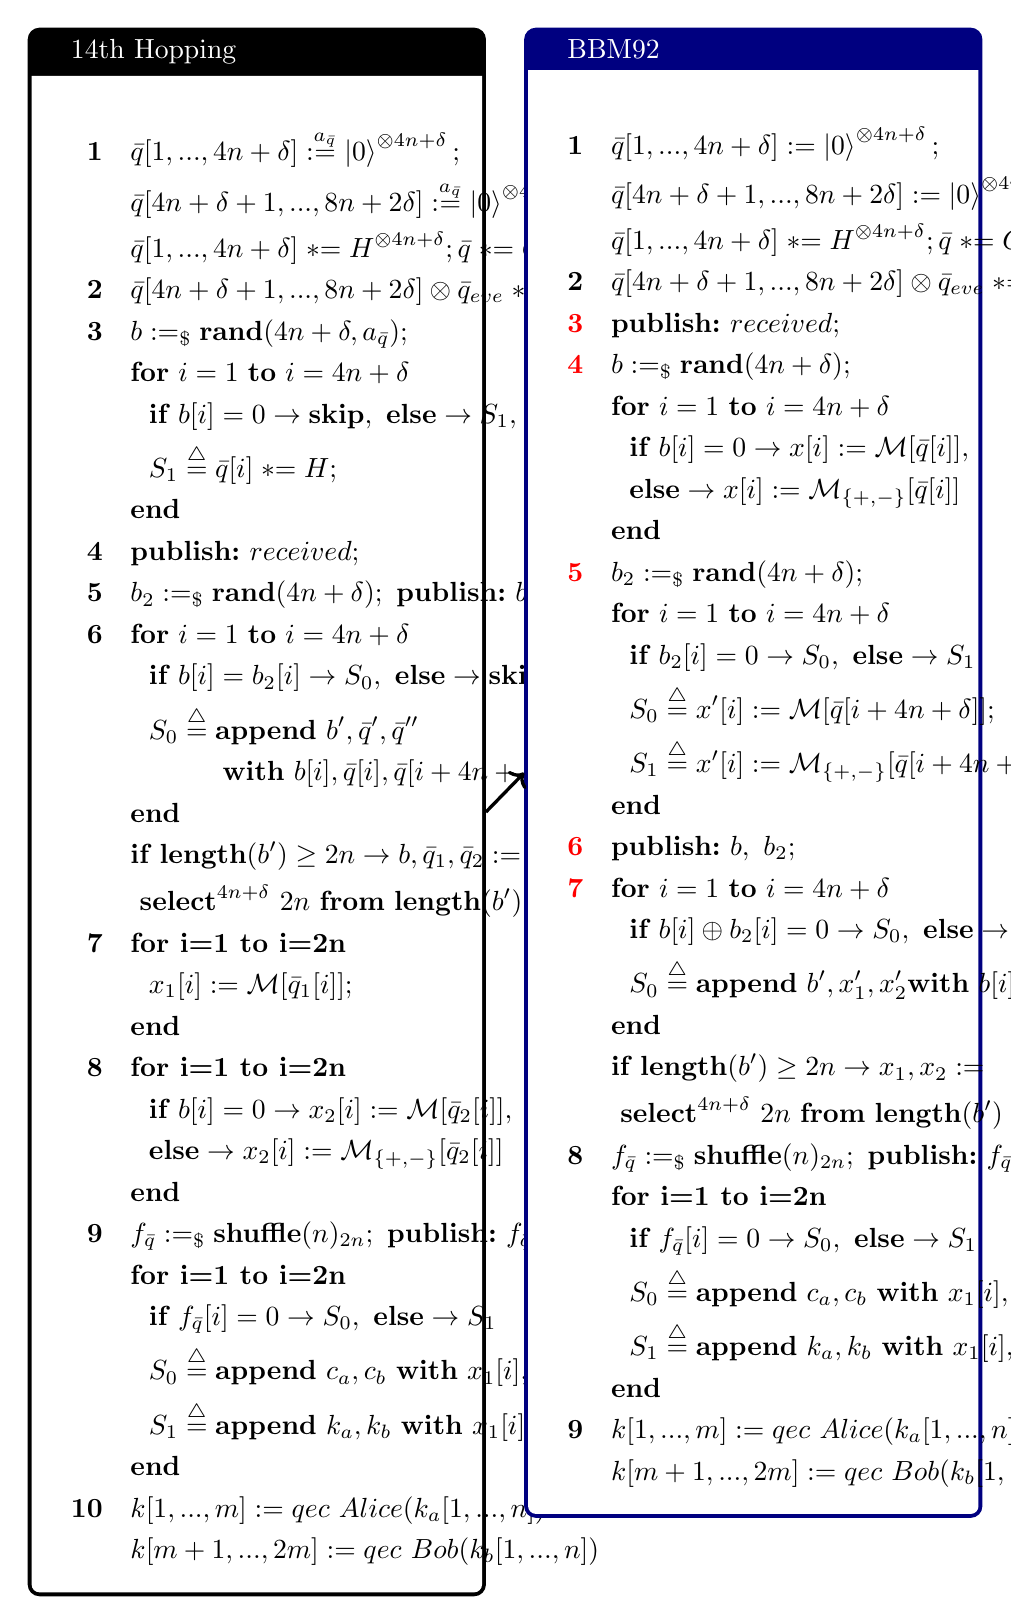
\begin{tikzpicture}[remember picture]

% Left box
\node[anchor=north west,inner sep=0pt,outer sep=0pt] (leftbox) at (0,0) {
\begin{minipage}[t]{0.48\textwidth}
\begin{tcolorbox}[colframe=black!50!black, colback=white, title=14th Hopping, width=\textwidth]
\begin{align*}
    {\textbf{1}} \quad 
    &\bar{q}[1,...,4n+\delta] :\stackrel{a_{\bar{q}}}{=} \ket{0}^{\otimes 4n+\delta}; \\
    &\bar{q}[4n+\delta+1,...,8n+2\delta] :\stackrel{a_{\bar{q}}}{=} \ket{0}^{\otimes 4n+\delta};\\
    \quad &\bar{q}[1,...,4n+\delta] \asteq H^{\otimes 4n+\delta}; \bar{q} \asteq CNOT; \\
    \textbf{2} \quad & \bar{q}[4n+\delta+1,...,8n+2\delta]\otimes \bar{q}_{eve} \asteq U_{\textbf{channel}}; \\
    {\textbf{3}} \quad & b :=_\$ \textbf{rand}(4n+\delta,a_{\bar{q}}); \\
    &\textbf{for}~i=1~\textbf{to}~i=4n+\delta\\
    &~~ \textbf{if }  b[i] = 0 \rightarrow \textbf{skip},~\textbf{else}\rightarrow S_{1},\\
    &~~ S_{1}\stackrel{\triangle}{=}\bar{q}[i] \asteq H ;\\
    &\textbf{end}\\
    \textbf{4} \quad & \textbf{publish:}~ received;\\
    {\textbf{5}} \quad & b_2 :=_\$ \textbf{rand}(4n+\delta); ~\textbf{publish:}~ b;\\
    {\textbf{6}} \quad &\textbf{for} ~i=1 ~\textbf{to} ~i=4n+\delta\\
    &~~ \textbf{if } b[i]= b_2[i] \rightarrow S_{0},~\textbf{else}\rightarrow\textbf{skip}~, \\
    &~~ S_{0}\stackrel{\triangle}{=}\textbf{append}~b',\bar{q}',\bar{q}''\\&~~~~~~~~~~\textbf{with}~b[i],\bar{q}[i],\bar{q}[i+4n+\delta];\\
    &\textbf{end}\\
    &{\textbf{if }} \textbf{length} (b')\geq 2n\rightarrow b,\bar{q}_1,\bar{q}_2:=\\&~\textbf{select}^{4n+\delta}~2n~\textbf{from}~\textbf{length}(b')~\textbf{for}~b',\bar{q}',\bar{q}'';\\
    {\textbf{{7}}} \quad & \textbf{for~i=1~to~i=2n}\\
    &~~ x_1[i]:= \mathcal{M} [\bar{q}_1[i]];\\
    &\textbf{end}\\
    {\textbf{{8}}} 
    \quad 
    &\textbf{for~i=1~to~i=2n}\\
    &~~ \textbf{if }  b[i] = 0 \rightarrow x_2[i]:= \mathcal{M} [\bar{q}_{2}[i]] ,\\
    &~~\textbf{else}\rightarrow x_2[i]:= \mathcal{M}_{\{+,-\}} [\bar{q}_{2}[i]]\\
    &\textbf{end}\\
    {\textbf{{9}}} \quad & f_{\bar{q}}:=_\$\textbf{shuffle}(n)_{2n}; ~ \textbf{publish:}~ f_{\bar{q}};\\ 
    &\textbf{for~i=1~to~i=2n}\\
    &~~ \textbf{if }  f_{\bar{q}}[i] = 0 \rightarrow S_{0},~\textbf{else}\rightarrow S_{1}\\
    &~~ S_{0}\stackrel{\triangle}{=}\textbf{append}~c_a,c_b~\textbf{with}~x_1[i],x_2[i];\\
    &~~ S_{1}\stackrel{\triangle}{=}\textbf{append}~k_a,k_b~\textbf{with}~x_1[i],x_2[i];\\
    &\textbf{end}\\
    \textbf{{10}} \quad & k[1,...,m]:=qec~Alice(k_a[1,...,n])\\
    \quad & k[m+1,...,2m]:=qec~Bob(k_b[1,...,n])
\end{align*}
\end{tcolorbox}
\end{minipage}
};

% Right box
\node[anchor=north west,inner sep=0pt,outer sep=0pt] (rightbox) at (0.52\textwidth,0) {
\begin{minipage}[t]{0.48\textwidth}
\begin{tcolorbox}[colframe=blue!50!black, colback=white, title=BBM92, width=\textwidth]
\begin{align*}
    \textbf{{1}} \quad 
    & \bar{q}[1,...,4n+\delta] := \ket{0}^{\otimes 4n+\delta}; \\
    &\bar{q}[4n+\delta+1,...,8n+2\delta] := \ket{0}^{\otimes 4n+\delta};\\
    \quad &\bar{q}[1,...,4n+\delta] \asteq H^{\otimes 4n+\delta}; \bar{q} \asteq CNOT; \\
    \textbf{{2}}\quad 
    & \bar{q}[4n+\delta+1,...,8n+2\delta]\otimes \bar{q}_{eve} \asteq U_{\textbf{channel}}; \\
    \textcolor{red}{\textbf{{3}}} 
    \quad &  \textbf{publish:}~ received;\\
    \textcolor{red}{\textbf{{4}}} \quad & b :=_\$ \textbf{rand}(4n+\delta);\\&\textbf{for} ~i=1 ~\textbf{to}~ i=4n+\delta\\
    &~~ \textbf{if }  b[i] = 0 \rightarrow x[i]:= \mathcal{M} [\bar{q}[i]] ,\\
    &~~\textbf{else}\rightarrow x[i]:= \mathcal{M}_{\{+,-\}} [\bar{q}[i]]\\
    &\textbf{end}\\
    \textcolor{red}{\textbf{{5}}} \quad &  b_2 :=_\$ \textbf{rand}(4n+\delta);\\&\textbf{for} ~i=1 ~\textbf{to}~ i=4n+\delta\\
    &~~ \textbf{if }  b_2[i] = 0 \rightarrow S_{0},~\textbf{else}\rightarrow S_{1}\\
    &~~ S_{0}\stackrel{\triangle}{=}x'[i]:= \mathcal{M} [\bar{q}[i+4n+\delta]];\\
    &~~ S_{1}\stackrel{\triangle}{=}x'[i]:= \mathcal{M}_{\{+,-\}} [\bar{q}[i+4n+\delta]];\\
    &\textbf{end}\\
    \textbf{\textcolor{red}{6}} \quad &\textbf{publish:}~ b,~b_2;\\
    \textbf{\textcolor{red}{7}} 
    \quad &\textbf{for} ~i=1 ~\textbf{to} ~i=4n+\delta\\
    &~~ \textbf{if } b[i]\oplus b_2[i]=0 \rightarrow S_{0},~\textbf{else}\rightarrow\textbf{skip}~, \\
    &~~ S_{0}\stackrel{\triangle}{=}\textbf{append}~b',x_1',x_2'\textbf{with}~b[i],x[i],x'[i];\\
    &\textbf{end}\\
    &{\textbf{if }} \textbf{length} (b')\geq 2n\rightarrow x_1,x_2:=\\&~\textbf{select}^{4n+\delta}~2n~\textbf{from}~\textbf{length}(b')~\textbf{for}~x_1',x_2';\\
    {\textbf{{8}}} \quad & f_{\bar{q}}:=_\$\textbf{shuffle}(n)_{2n}; ~ \textbf{publish:}~ f_{\bar{q}};\\ 
    &\textbf{for~i=1~to~i=2n}\\
    &~~ \textbf{if }  f_{\bar{q}}[i] = 0 \rightarrow S_{0},~\textbf{else}\rightarrow S_{1}\\
    &~~ S_{0}\stackrel{\triangle}{=}\textbf{append}~c_a,c_b~\textbf{with}~x_1[i],x_2[i];\\
    &~~ S_{1}\stackrel{\triangle}{=}\textbf{append}~k_a,k_b~\textbf{with}~x_1[i],x_2[i];\\
    &\textbf{end}\\
    \textbf{{9}} \quad & k[1,...,m]:=qec~Alice(k_a[1,...,n])\\
    \quad & k[m+1,...,2m]:=qec~Bob(k_b[1,...,n])
\end{align*}
\end{tcolorbox}
\end{minipage}
};

% Draw arrow between boxes
\draw[->, very thick] (leftbox.east) -- node[above]{} (rightbox.west);

\end{tikzpicture}
\newpage

\end{document}
